\documentclass[11pt]{book}

\usepackage{cite} 
\usepackage[pdftex]{graphicx}
\usepackage{titlesec}
\usepackage{listings}
\usepackage{fancyvrb}
\usepackage[svgnames]{xcolor}
\usepackage{framed}
\usepackage{amsmath}
\usepackage{amssymb}
\usepackage{bbm}
\usepackage{hyperref}
\usepackage{makeidx}
\usepackage{color}

\definecolor{shadecolor}{gray}{0.95}  % Background color of title bars
\lstset{
language=C,
basicstyle=\small\ttfamily,
backgroundcolor=\color{shadecolor}
}

\makeindex

\newcommand{\piRsquare}{\pi r^2}		% This is my own macro !!!

\usepackage{helvetica}
\usepackage{ifthen}
\usepackage{alltt}
\usepackage{opencv}

%%% Margins %%%
\oddsidemargin 0.0in
\evensidemargin 0.0in
\textwidth 6.5in
%\headheight 1.0in
%\topmargin 0.5in
%\textheight 9.0in
%\footheight 1.0in 
%%%%%%%%%%%%%%%

\title{OpenCV Documentation}			% used by \maketitle
\author{Authors}		% used by \maketitle
\date{May 7, 2009}					% used by \maketitle

\begin{document}
\maketitle						% automatic title!

\setcounter{tocdepth}{8}
\tableofcontents

\titleformat{\subsubsection}
{\titlerule
\vspace{.8ex}%
\normalfont\bfseries\Large}
{\thesection.}{.5em}{}

%%% Define these to get rid of warnings
\def\genc{true}
\def\genpy{true}

%%% Chapters %%%
\include{CxCore-c}
\include{CvReference-c}
\chapter{CvAux}

\section{Stereo Correspondence Functions}

\cvfunc{FindStereoCorrespondence} % XXX No images at source url's

Calculates disparity for stereo-pair

\cvexp{
cvFindStereoCorrespondence(
                   \par const  CvArr* leftImage, \par const  CvArr* rightImage,
                   \par int     mode, \par CvArr*  depthImage,
                   \par int     maxDisparity,
                   \par double  param1, \par double  param2, \par double  param3,
                   \par double  param4, \par double  param5  );

}{CPP}{PYTHON}

\begin{description}
\cvarg{leftImage}{Left image of stereo pair, rectified grayscale 8-bit imagerightImage}
\cvarg{rightImage}{Right image of stereo pair, rectified grayscale 8-bit imagemode}
\cvarg{mode}{Algorithm used to find a disparity (now only CV\_DISPARITY\_BIRCHFIELD is supported)}
\cvarg{depthImage}{Destination depth image, grayscale 8-bit image that codes the scaled disparity, so that the zero disparity (corresponding to the points that are very far from the cameras) maps to 0, maximum disparity maps to 255.}
\cvarg{maxDisparity}{Maximum possible disparity. The closer the objects to the cameras, the larger value should be specified here. Too big values slow down the process significantly.}
\cvarg{param1, param2, param3, param4, param5}{- parameters of algorithm. For example, param1 is the constant occlusion penalty, param2 is the constant match reward, param3 defines a highly reliable region (set of contiguous pixels whose reliability is at least param3), param4 defines a moderately reliable region, param5 defines a slightly reliable region. If some parameter is omitted default value is used. In Birchfield's algorithm param1 = 25, param2 = 5, param3 = 12, param4 = 15, param5 = 25 (These values have been taken from "Depth Discontinuities by Pixel-to-Pixel Stereo" Stanford University Technical Report STAN-CS-TR-96-1573, July 1996.)}
\end{description}

The function \texttt{cvFindStereoCorrespondence} calculates disparity map for two rectified grayscale images.

Example. Calculating disparity for pair of 8-bit color images

\begin{lstlisting}
/*---------------------------------------------------------------------------------*/
IplImage* srcLeft = cvLoadImage("left.jpg",1);
IplImage* srcRight = cvLoadImage("right.jpg",1);
IplImage* leftImage = cvCreateImage(cvGetSize(srcLeft), IPL\_DEPTH\_8U, 1);
IplImage* rightImage = cvCreateImage(cvGetSize(srcRight), IPL\_DEPTH\_8U, 1);
IplImage* depthImage = cvCreateImage(cvGetSize(srcRight), IPL\_DEPTH\_8U, 1);

cvCvtColor(srcLeft, leftImage, CV\_BGR2GRAY);
cvCvtColor(srcRight, rightImage, CV\_BGR2GRAY);

cvFindStereoCorrespondence( leftImage, rightImage, CV\_DISPARITY\_BIRCHFIELD, depthImage, 50, 15, 3, 6, 8, 15 );
/*---------------------------------------------------------------------------------*/

\end{lstlisting}

And here is the example stereo pair that can be used to test the example

\begin{lstlisting}
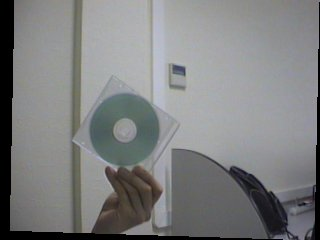
\includegraphics{http://opencvlibrary.sourceforge.net/pics/left.jpg} 
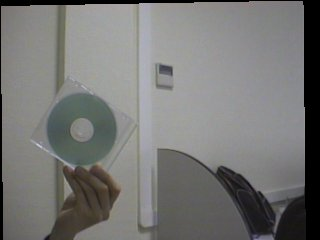
\includegraphics{http://opencvlibrary.sourceforge.net/pics/right.jpg}
\end{lstlisting}

\section{View Morphing Functions}

\cvfunc{MakeScanlines}

Calculates scanlines coordinates for two cameras by fundamental matrix

\cvexp{
void cvMakeScanlines( \par const CvMatrix3* matrix, \par CvSize img\_size, \par int* scanlines1,
                      \par int* scanlines2, \par int* lengths1, \par int* lengths2, \par int* line\_count );

}{CPP}{PYTHON}

\begin{description}
\cvarg{matrix}{Fundamental matrix.}
\cvarg{imgSize}{Size of the image.}
\cvarg{scanlines1}{Pointer to the array of calculated scanlines of the first image.}
\cvarg{scanlines2}{Pointer to the array of calculated scanlines of the second image.}
\cvarg{lengths1}{Pointer to the array of calculated lengths (in pixels) of the first image scanlines.}
\cvarg{lengths2}{Pointer to the array of calculated lengths (in pixels) of the second image scanlines.}
\cvarg{line\_count}{Pointer to the variable that stores the number of scanlines.}
\end{description}

The function \texttt{cvMakeScanlines} finds coordinates of scanlines for two images.

This function returns the number of scanlines. The function does nothing except calculating the number of scanlines if the pointers \texttt{scanlines1} or \texttt{scanlines2} are equal to zero.

\cvfunc{PreWarpImage}

Rectifies image

\cvexp{
void cvPreWarpImage( \par int line\_count, \par IplImage* img, \par uchar* dst,
                     \par int* dst\_nums, \par int* scanlines );

}{CPP}{PYTHON}

\begin{description}
\cvarg{line\_count}{Number of scanlines for the image.}
\cvarg{img}{Image to prewarp.}
\cvarg{dst}{Data to store for the prewarp image.}
\cvarg{dst\_nums}{Pointer to the array of lengths of scanlines.}
\cvarg{scanlines}{Pointer to the array of coordinates of scanlines.}
\end{description}

The function \texttt{cvPreWarpImage} rectifies the image so that the scanlines in the rectified image are horizontal. The output buffer of size \texttt{max(width,height)*line\_count*3} must be allocated before calling the function.

\cvfunc{FindRuns}

Retrieves scanlines from rectified image and breaks them down into runs

\cvexp{
void cvFindRuns( \par int line\_count, \par uchar* prewarp1, \par uchar* prewarp2,
                 \par int* line\_lengths1, \par int* line\_lengths2,
                 \par int* runs1, \par int* runs2,
                 \par int* num\_runs1, \par int* num\_runs2 );

}{CPP}{PYTHON}

\begin{description}
\cvarg{line\_count}{Number of the scanlines.}
\cvarg{prewarp1}{Prewarp data of the first image.}
\cvarg{prewarp2}{Prewarp data of the second image}.
\cvarg{line\_lengths1}{Array of lengths of scanlines in the first image.}
\cvarg{line\_lengths2}{Array of lengths of scanlines in the second image.}
\cvarg{runs1}{Array of runs in each scanline in the first image.}
\cvarg{runs2}{Array of runs in each scanline in the second image.}
\cvarg{num\_runs1}{Array of numbers of runs in each scanline in the first image.}
\cvarg{num\_runs2}{Array of numbers of runs in each scanline in the second image.}
\end{description}

The function \texttt{cvFindRuns} retrieves scanlines from the rectified image and breaks each scanline down into several runs, that is, series of pixels of almost the same brightness.

\cvfunc{DynamicCorrespondMulti}

Finds correspondence between two sets of runs of two warped images

\cvexp{
void cvDynamicCorrespondMulti( \par int line\_count, \par int* first, \par int* first\_runs,
                               \par int* second, \par int* second\_runs,
                               \par int* first\_corr, \par int* second\_corr );

}{CPP}{PYTHON}

\begin{description}
\cvarg{line\_count}{Number of scanlines.}
\cvarg{first}{Array of runs of the first image.}
\cvarg{first\_runs}{Array of numbers of runs in each scanline of the first image.}
\cvarg{second}{Array of runs of the second image.}
\cvarg{second\_runs}{Array of numbers of runs in each scanline of the second image.}
\cvarg{first\_corr}{Pointer to the array of correspondence information found for the first runs.}
\cvarg{second\_corr}{Pointer to the array of correspondence information found for the second runs.}
\end{description}

The function \texttt{cvDynamicCorrespondMulti} finds correspondence between two sets of runs of two images. Memory must be allocated before calling this function. Memory size for one array of correspondence information is

\texttt{max( width,height )* numscanlines*3*sizeof ( int ).} 


\cvfunc{MakeAlphaScanlines}

Calculates coordinates of scanlines of image from virtual camera

\cvexp{
void cvMakeAlphaScanlines( \par int* scanlines1, \par int* scanlines2,
                           \par int* scanlinesA, \par int* lengths,
                           \par int line\_count, \par float alpha );

}{CPP}{PYTHON}

\begin{description}
\cvarg{scanlines1}{Pointer to the array of the first scanlines.}
\cvarg{scanlines2}{Pointer to the array of the second scanlines.}
\cvarg{scanlinesA}{Pointer to the array of the scanlines found in the virtual image.}
\cvarg{lengths}{Pointer to the array of lengths of the scanlines found in the virtual image.}
\cvarg{line\_count}{Number of scanlines.}
\cvarg{alpha}{Position of virtual camera \texttt{($0.0 - 1.0$)}.} 
\end{description}

The function \texttt{cvMakeAlphaScanlines} finds coordinates of scanlines for the virtual camera with the given camera position.

Memory must be allocated before calling this function. Memory size for the array of correspondence runs is \texttt{numscanlines*2*4*sizeof(int)}. Memory size for the array of the scanline lengths is \texttt{numscanlines*2*4*sizeof(int).}

\cvfunc{MorphEpilinesMulti}

Morphs two pre-warped images using information about stereo correspondence

\cvexp{
void cvMorphEpilinesMulti( \par int line\_count, \par uchar* first\_pix, \par int* first\_num,
                           \par uchar* second\_pix, \par int* second\_num,
                           \par uchar* dst\_pix, \par int* dst\_num,
                           \par float alpha, \par int* first, \par int* first\_runs,
                           \par int* second, \par int* second\_runs,
                           \par int* first\_corr, \par int* second\_corr );

}{CPP}{PYTHON}

\begin{description}
\cvarg{line\_count}{Number of scanlines in the prewarp image.}
\cvarg{first\_pix}{Pointer to the first prewarp image.}
\cvarg{first\_num}{Pointer to the array of numbers of points in each scanline in the first image.}
\cvarg{second\_pix}{Pointer to the second prewarp image.}
\cvarg{second\_num}{Pointer to the array of numbers of points in each scanline in the second image.}
\cvarg{dst\_pix}{Pointer to the resulting morphed warped image.}
\cvarg{dst\_num}{Pointer to the array of numbers of points in each line.}
\cvarg{alpha}{Virtual camera position \texttt{($0.0 - 1.0$)}.}
\cvarg{first}{First sequence of runs.}
\cvarg{first\_runs}{Pointer to the number of runs in each scanline in the first image.}
\cvarg{second}{Second sequence of runs.}
\cvarg{second\_runs}{Pointer to the number of runs in each scanline in the second image.}
\cvarg{first\_corr}{Pointer to the array of correspondence information found for the first runs.}
\cvarg{second\_corr}{Pointer to the array of correspondence information found for the second runs.}
\end{description}

The function \texttt{cvMorphEpilinesMulti} morphs two pre-warped images using information about correspondence between the scanlines of two images.

\cvfunc{PostWarpImage}

Warps rectified morphed image back

\cvexp{
void cvPostWarpImage( \par int line\_count, \par uchar* src, \par int* src\_nums,
                      \par IplImage* img, \par int* scanlines );

}{CPP}{PYTHON}

\begin{description}
\cvarg{line\_count}{Number of the scanlines.}
\cvarg{src}{Pointer to the prewarp image virtual image.}
\cvarg{src\_nums}{Number of the scanlines in the image.}
\cvarg{img}{Resulting unwarp image.}
\cvarg{scanlines}{Pointer to the array of scanlines data.}
\end{description}

The function \texttt{cvPostWarpImage} warps the resultant image from the virtual camera by storing its rows across the scanlines whose coordinates are calculated by \cross{MakeAlphaScanlines}.

\cvfunc{DeleteMoire}

Deletes moire in given image

\cvexp{
void cvDeleteMoire( IplImage* img );

}{CPP}{PYTHON}

\begin{description}
\cvarg{img}{Image.}
\end{description}

The function \texttt{cvDeleteMoire} deletes moire from the given image. The post-warped image may have black (un-covered) points because of possible holes between neighboring scanlines. The function deletes moire (black pixels) from the image by substituting neighboring pixels for black pixels. If all the scanlines are horizontal, the function may be omitted.

\section{3D Tracking Functions} % XXX Weird URL Formatting, /../?

The section discusses functions for tracking objects in 3d space using a stereo camera. Besides C API, there is DirectShow
\url{http://opencvlibrary.sourceforge.net/../appPage/3dTracker/3dTrackerFilter.htm}
filter and the wrapper application
\url{http://opencvlibrary.sourceforge.net/../appPage/3dTracker/3dTracker.htm}.
\url{http://opencvlibrary.sourceforge.net/../appPage/3dTracker/3dTrackerTesting.htm} you may find a description how to test the filter on sample data.

\cvfunc{3dTrackerCalibrateCameras} % XXX URL Formatting

Simultaneously determines position and orientation of multiple cameras

\cvexp{
CvBool cv3dTrackerCalibrateCameras(\par int num\_cameras,
           \par const Cv3dTrackerCameraIntrinsics camera\_intrinsics[],
           \par CvSize checkerboard\_size,
           \par IplImage *samples[],
           \par Cv3dTrackerCameraInfo camera\_info[]);

}{CPP}{PYTHON}

\begin{description}
\cvarg{num\_cameras}{the number of cameras to calibrate. This is the size of each of the three array parameters.}
\cvarg{camera\_intrinsics}{camera intrinsics for each camera, such as determined by CalibFilter.}
\cvarg{checkerboard\_size}{the width and height (in number of squares) of the checkerboard.}
\cvarg{samples}{images from each camera, with a view of the checkerboard.}
\cvarg{camera\_info}{filled in with the results of the camera calibration. This is passed into \cross{3dTrackerLocateObjects} to do tracking.}
\end{description}

The function \texttt{cv3dTrackerCalibrateCameras} searches for a checkerboard of the specified size in each of the images. For each image in which it finds the checkerboard, it fills in the corresponding slot in \texttt{camera\_info} with the position and orientation of the camera relative to the checkerboard and sets the \texttt{valid} flag. If it finds the checkerboard in all the images, it returns true; otherwise it returns false.

This function does not change the members of the \texttt{camera\_info} array that correspond to images in which the checkerboard was not found. This allows you to calibrate each camera independently, instead of simultaneously. To accomplish this, do the following:
\begin{enumerate}
\item Clear all the \texttt{valid} flags before calling this function the first time;
\item Call this function with each set of images;
\item Check all the \texttt{valid} flags after each call. When all the \texttt{valid} flags are set, calibration is complete.
\end{enumerate}

Note that this method works well only if the checkerboard is rigidly mounted; if it is handheld, all the cameras should be calibrated simultanously to get an accurate result. To ensure that all cameras are calibrated simultaneously, ignore the \texttt{valid} flags and use the return value to decide when calibration is complete.

\cvfunc{3dTrackerLocateObjects}

Determines 3d location of tracked objects

\cvexp{
int  cv3dTrackerLocateObjects(\par int num\_cameras,
         \par int num\_objects,
         \par const Cv3dTrackerCameraInfo camera\_info[],
         \par const Cv3dTracker2dTrackedObject tracking\_info[],
         \par Cv3dTrackerTrackedObject tracked\_objects[]);

}{CPP}{PYTHON}

\begin{description}
\cvarg{num\_cameras}{the number of cameras.}
\cvarg{num\_objects}{the maximum number of objects found by any camera. (Also the maximum number of objects returned in \texttt{tracked\_objects}.}
\cvarg{camera\_info}{camera position and location information for each camera, as determined by \cross{3dTrackerCalibrateCameras}.}
\cvarg{tracking\_info}{the 2d position of each object as seen by each camera. Although this is specified as a one-dimensional array, it is actually a two-dimensional array: \texttt{const Cv3dTracker2dTrackedObject tracking\_info[num\_cameras][num\_objects]}. The \texttt{id} field of any unused slots must be $-1$. Ids need not be ordered or consecutive.}
\cvarg{tracked\_objects}{filled in with the results.}
\end{description}

The function \texttt{cv3dTrackerLocateObjects} determines the 3d position of tracked objects based on the 2d tracking information from multiple cameras and the camera position and orientation information computed by \cross{3dTrackerCalibrateCameras}. It locates any objects with the same \texttt{id} that are tracked by more than one camera. It fills in the \texttt{tracked\_objects} array and returns the number of objects located. The \texttt{id} fields of any unused slots in \texttt{tracked\_objects} are set to $-1$.

\section{Eigen Objects (PCA) Functions}

The functions described in this section do PCA analysis
and compression for a set of 8-bit images that may not fit
into memory all together. If your data fits into memory and
the vectors are not 8-bit (or you want a simpler interface), use
\cross{CalcCovarMatrix},
\cross{SVD}
and
\cross{GEMM}
to do PCA.

\cvfunc{CalcCovarMatrixEx}

Calculates covariance matrix for group of input objects

\cvexp{
void cvCalcCovarMatrixEx( \par int object\_count, \par void* input, \par int io\_flags,
                          \par int iobuf\_size, \par uchar* buffer, \par void* userdata,
                          \par IplImage* avg, \par float* covar\_matrix );

}{CPP}{PYTHON}

\begin{description}
\cvarg{object\_count}{Number of source objects.}
\cvarg{input}{Pointer either to the array of \texttt{IplImage} input objects or to the read callback function according to the value of the parameter \texttt{ioFlags}.}
\cvarg{io\_flags}{Input/output flags.}
\cvarg{iobuf\_size}{Input/output buffer size.}
\cvarg{buffer}{Pointer to the input/output buffer.}
\cvarg{userdata}{Pointer to the structure that contains all necessary data for the callback functions.}
\cvarg{avg}{Averaged object.}
\cvarg{covar\_matrix}{Covariance matrix. An output parameter; must be allocated before the call.}
\end{description}

The function \texttt{cvCalcCovarMatrixEx} calculates a covariance matrix of the input objects group using previously calculated averaged object. Depending on \texttt{ioFlags} parameter it may be used either in direct access or callback mode. If \texttt{ioFlags} is not \texttt{CV\_EIGOBJ\_NO\_CALLBACK}, buffer must be allocated before calling the function.

\cvfunc{CalcEigenObjects}

Calculates orthonormal eigen basis and averaged object for group of input objects

\cvexp{
void cvCalcEigenObjects( \par int nObjects, \par void* input, \par void* output, \par int ioFlags,
                         \par int ioBufSize, \par void* userData, \par CvTermCriteria* calcLimit,
                         \par IplImage* avg, \par float* eigVals );

}{CPP}{PYTHON}

\begin{description}
\cvarg{nObjects}{Number of source objects.}
\cvarg{input}{Pointer either to the array of \texttt{IplImage} input objects or to the read callback function according to the value of the parameter \texttt{ioFlags}.}
\cvarg{output}{Pointer either to the array of eigen objects or to the write callback function according to the value of the parameter ioFlags.}
\cvarg{ioFlags}{Input/output flags.}
\cvarg{ioBufSize}{Input/output buffer size in bytes. The size is zero, if unknown.}
\cvarg{userData}{Pointer to the structure that contains all necessary data for the callback functions.}
\cvarg{calcLimit}{Criteria that determine when to stop calculation of eigen objects.}
\cvarg{avg}{Averaged object.}
\cvarg{eigVals}{Pointer to the eigenvalues array in the descending order; may be \texttt{NULL}.}
\end{description}

The function \texttt{cvCalcEigenObjects} calculates orthonormal eigen basis and the averaged object for a group of the input objects. Depending on \texttt{ioFlags} parameter it may be used either in direct access or callback mode. Depending on the parameter \texttt{calcLimit}, calculations are finished either after first \texttt{calcLimit.max\_iter} dominating eigen objects are retrieved or if the ratio of the current eigenvalue to the largest eigenvalue comes down to \texttt{calcLimit.epsilon} threshold. The value \texttt{calcLimit -> type} must be \texttt{CV\_TERMCRIT\_NUMB, CV\_TERMCRIT\_EPS}, or \texttt{CV\_TERMCRIT\_NUMB | CV\_TERMCRIT\_EPS} . The function returns the real values \texttt{calcLimit->max\_iter} and \texttt{calcLimit->epsilon} .

The function also calculates the averaged object, which must be created previously. Calculated eigen objects are arranged according to the corresponding eigenvalues in the descending order.

The parameter \texttt{eigVals} may be equal to \texttt{NULL}, if eigenvalues are not needed.

The function \texttt{cvCalcEigenObjects} uses the function \cross{cvCalcCovarMatrixEx}.

\cvfunc{CalcDecompCoeff}

Calculates decomposition coefficient of input object

\cvexp{
double cvCalcDecompCoeff( \par IplImage* obj, \par IplImage* eigObj, \par IplImage* avg );

}{CPP}{PYTHON}

\begin{description}
\cvarg{obj}{Input object.}
\cvarg{eigObj}{Eigen object.}
\cvarg{avg}{Averaged object.}
\end{description}

The function \texttt{cvCalcDecompCoeff} calculates one decomposition coefficient of the input object using the previously calculated eigen object and the averaged object.

\cvfunc{EigenDecomposite}

Calculates all decomposition coefficients for input object

\cvexp{
void cvEigenDecomposite( \par IplImage* obj, \par int eigenvec\_count, \par void* eigInput,
                         \par int ioFlags, \par void* userData, \par IplImage* avg, \par float* coeffs );

}{CPP}{PYTHON}

\begin{description}
\cvarg{obj}{Input object.}
\cvarg{eigenvec\_count}{Number of eigen objects.}
\cvarg{eigInput}{Pointer either to the array of \texttt{IplImage} input objects or to the read callback function according to the value of the parameter \texttt{ioFlags}.}
\cvarg{ioFlags}{Input/output flags.}
\cvarg{userData}{Pointer to the structure that contains all necessary data for the callback functions.}
\cvarg{avg}{Averaged object.}
\cvarg{coeffs}{Calculated coefficients; an output parameter.}
\end{description}

The function \texttt{cvEigenDecomposite} calculates all decomposition coefficients for the input object using the previously calculated eigen objects basis and the averaged object. Depending on \texttt{ioFlags} parameter it may be used either in direct access or callback mode.

\cvfunc{EigenProjection}

Calculates object projection to the eigen sub-space

\cvexp{
void cvEigenProjection( \par void* input\_vecs, \par int eigenvec\_count, \par int io\_flags, \par void* userdata,
                        \par float* coeffs, \par IplImage* avg, \par IplImage* proj );

}{CPP}{PYTHON}

\begin{description}
\cvarg{input\_vec}{Pointer to either an array of \texttt{IplImage} input objects or to a callback function, depending on \texttt{io\_flags}.}
\cvarg{eigenvec\_count}{Number of eigenvectors.}
\cvarg{io\_flags}{Input/output flags; see \cross{cvCalcEigenObjects}.}
\cvarg{userdata}{Pointer to the structure that contains all necessary data for the callback functions.}
\cvarg{coeffs}{Previously calculated decomposition coefficients.}
\cvarg{avg}{Average vector, calculated by \cross{cvCalcEigenObjects}.}
\cvarg{proj}{Projection to the eigen sub-space.}
\end{description}

The function \texttt{cvEigenProjection} calculates an object projection to the eigen sub-space or, in other words, restores an object using previously calculated eigen objects basis, averaged object, and decomposition coefficients of the restored object. Depending on \texttt{io\_flags} parameter it may be used either in direct access or callback mode.

\section{Embedded Hidden Markov Models Functions}

In order to support embedded models the user must define structures to represent 1D HMM and 2D embedded HMM model.

\cvfunc{CvHMM} 

Embedded HMM Structure

\cvexp{typedef struct \_CvEHMM}{CPP}{PYTHON}
\begin{lstlisting} 
    {
        int level;
        int num_states;
        float* transP;
        float** obsProb;
        union
        {
            CvEHMMState* state;
            struct _CvEHMM* ehmm;
        } u;
    } CvEHMM;
\end{lstlisting}


\begin{description}
\cvarg{level}{Level of embedded HMM. If \texttt{level $==0$}, HMM is most external. In 2D HMM there are two types of HMM: 1 external and several embedded. External HMM has \texttt{level $==1$}, embedded HMMs have \texttt{level $==0$}.}
\cvarg{num\_states}{Number of states in 1D HMM.}
\cvarg{transP}{State-to-state transition probability, square matrix \texttt{(num\_state×num\_state )}.}
\cvarg{obsProb}{Observation probability matrix.}
\cvarg{state}{Array of HMM states. For the last-level HMM, that is, an HMM without embedded HMMs, HMM states are real.}
\cvarg{ehmm}{Array of embedded HMMs. If HMM is not last-level, then HMM states are not real and they are HMMs.}
\end{description}

For representation of observations the following structure is defined:

\cvfunc{CvImgObsInfo}

Image Observation Structure

\cvexp{
    typedef struct CvImgObsInfo
    }{CPP}{PYTHON}
\begin{lstlisting}
    {
        int obs_x;
        int obs_y;
        int obs_size;
        float** obs;
        int* state;
        int* mix;
    } CvImgObsInfo;
\end{lstlisting}

\begin{description}
\cvarg{obs\_x}{Number of observations in the horizontal direction.}
\cvarg{obs\_y}{Number of observations in the vertical direction.}
\cvarg{obs\_size}{Length of every observation vector.}
\cvarg{obs}{Pointer to observation vectors stored consequently. Number of vectors is \texttt{obs\_x*obs\_y}.}
\cvarg{state}{Array of indices of states, assigned to every observation vector.}
\cvarg{mix}{Index of mixture component, corresponding to the observation vector within an assigned state.}
\end{description}

\cvfunc{Create2DHMM}

Creates 2D embedded HMM

\cvexp{
CvEHMM* cvCreate2DHMM( int* stateNumber, int* numMix, int obsSize );

}{CPP}{PYTHON}

\begin{description}
\cvarg{stateNumber}{Array, the first element of the which specifies the number of superstates in the HMM. All subsequent elements specify the number of states in every embedded HMM, corresponding to each superstate. So, the length of the array is \texttt{stateNumber [$0$]+$1$}.}
\cvarg{numMix}{Array with numbers of Gaussian mixture components per each internal state. The number of elements in the array is equal to number of internal states in the HMM, that is, superstates are not counted here.}
\cvarg{obsSize}{Size of observation vectors to be used with created HMM.}
\end{description}

The function \texttt{cvCreate2DHMM} returns the created structure of the type \cross{CvEHMM} with specified parameters.

\cvfunc{Release2DHMM}

Releases 2D embedded HMM

\cvexp{
void cvRelease2DHMM(CvEHMM** hmm );

}{CPP}{PYTHON}

\begin{description}
\cvarg{hmm}{Address of pointer to HMM to be released.}
\end{description}

The function \texttt{cvRelease2DHMM} frees all the memory used by HMM and clears the pointer to HMM.

\cvfunc{CreateObsInfo}

Creates structure to store image observation vectors

\cvexp{
CvImgObsInfo* cvCreateObsInfo( CvSize numObs, int obsSize );

}{CPP}{PYTHON}

\begin{description}
\cvarg{numObs}{Numbers of observations in the horizontal and vertical directions. For the given image and scheme of extracting observations the parameter can be computed via the macro \texttt{CV\_COUNT\_OBS( roi, dctSize, delta, numObs )}, where \texttt{roi, dctSize, delta, numObs} are the pointers to structures of the type \cross{CvSize}. The pointer \texttt{roi} means size of \texttt{roi} of image observed, \texttt{numObs} is the output parameter of the macro.}
\cvarg{obsSize}{Size of observation vectors to be stored in the structure.}
\end{description}

The function \texttt{cvCreateObsInfo} creates new structures to store image observation vectors. For definitions of the parameters \texttt{roi, dctSize}, and \texttt{delta} see the specification of The function \texttt{cvImgToObs\_DCT}.

\cvfunc{ReleaseObsInfo}

Releases observation vectors structure

\cvexp{
void cvReleaseObsInfo( CvImgObsInfo** obsInfo );

}{CPP}{PYTHON}

\begin{description}
\cvarg{obsInfo}{Address of the pointer to the structure \cross{CvImgObsInfo}.}
\end{description}

The function \texttt{cvReleaseObsInfo} frees all memory used by observations and clears pointer to the structure \cross{CvImgObsInfo}.

\cvfunc{ImgToObs\_DCT}

Extracts observation vectors from image

\cvexp{
void cvImgToObs\_DCT( \par IplImage* image, \par float* obs, \par CvSize dctSize,
                     \par CvSize obsSize, \par CvSize delta );

}{CPP}{PYTHON}

\begin{description}
\cvarg{image}{Input image.}
\cvarg{obs}{Pointer to consequently stored observation vectors.}
\cvarg{dctSize}{Size of image blocks for which DCT (Discrete Cosine Transform) coefficients are to be computed.}
\cvarg{obsSize}{Number of the lowest DCT coefficients in the horizontal and vertical directions to be put into the observation vector.}
\cvarg{delta}{Shift in pixels between two consecutive image blocks in the horizontal and vertical directions.}
\end{description}

The function \texttt{cvImgToObs\_DCT} extracts observation vectors, that is, DCT coefficients, from the image. The user must pass \texttt{obsInfo.obs} as the parameter \texttt{obs} to use this function with other HMM functions and use the structure \texttt{obsInfo} of the \cross{CvImgObsInfo} type.

\texttt{Calculating Observations for HMM}

\cvexp{
    CvImgObsInfo* obs\_info;

        ...

        cvImgToObs\_DCT( image,obs\_info->obs, //!!!

        dctSize, obsSize, delta );

}{CPP}{PYTHON}

\cvfunc{UniformImgSegm} % XXX Picture not at link

Performs uniform segmentation of image observations by HMM states

\cvexp{
void cvUniformImgSegm( CvImgObsInfo* obsInfo, CvEHMM* hmm );

}{CPP}{PYTHON}

\begin{description}
\cvarg{obsInfo}{Observations structure.}
\cvarg{hmm}{HMM structure.}
\end{description}

The function \texttt{cvUniformImgSegm} segments image observations by HMM states uniformly (see \textcolor{blue}{\underline{Initial Segmentation}} for 2D Embedded HMM for 2D embedded HMM with 5 superstates and 3, 6, 6, 6, 3 internal states of every corresponding superstate).

\textcolor{blue}{Initial Segmentation for 2D Embedded HMM}

\url{http://opencvlibrary.sourceforge.net/pics/face.png}

\cvfunc{InitMixSegm}

Segments all observations within every internal state of HMM by state mixture components

\cvexp{
void cvInitMixSegm( \par CvImgObsInfo** obsInfoArray, \par int numImg, \par CvEHMM* hmm );

}{CPP}{PYTHON}

\begin{description}
\cvarg{obsInfoArray}{Array of pointers to the observation structures.}
\cvarg{numImg}{Length of above array.}
\cvarg{hmm}{HMM.}
\end{description}

The function \texttt{cvInitMixSegm} takes a group of observations from several training images already segmented by states and splits a set of observation vectors within every internal HMM state into as many clusters as the number of mixture components in the state.

\cvfunc{EstimateHMMStateParams}

Estimates all parameters of every HMM state

\cvexp{
void cvEstimateHMMStateParams( \par CvImgObsInfo** obsInfoArray, \par int numImg, \par CvEHMM* hmm );

}{CPP}{PYTHON}

\begin{description}
\cvarg{obsInfoArray}{Array of pointers to the observation structures.}
\cvarg{numImg}{Length of the array.}
\cvarg{hmm}{HMM.}
\end{description}

The function \texttt{cvEstimateHMMStateParams} computes all inner parameters of every HMM state, including Gaussian means, variances, etc.

\cvfunc{EstimateTransProb}

Computes transition probability matrices for embedded HMM

\cvexp{
void cvEstimateTransProb( \par CvImgObsInfo** obsInfoArray, \par int numImg, \par CvEHMM* hmm );

}{CPP}{PYTHON}

\begin{description}
\cvarg{obsInfoArray}{Array of pointers to the observation structures.}
\cvarg{numImg}{Length of the above array.}
\cvarg{hmm}{HMM.}
\end{description}

The function \texttt{cvEstimateTransProb} uses current segmentation of image observations to compute transition probability matrices for all embedded and external HMMs.

\cvfunc{EstimateObsProb}

Computes probability of every observation of several images

\cvexp{
void cvEstimateObsProb( CvImgObsInfo* obsInfo, CvEHMM* hmm );

}{CPP}{PYTHON}

\begin{description}
\cvarg{obsInfo}{Observation structure.}
\cvarg{hmm}{HMM structure.}
\end{description}

The function \texttt{cvEstimateObsProb} computes Gaussian probabilities of each observation to occur in each of the internal HMM states.

\cvfunc{EViterbi}

Executes Viterbi algorithm for embedded HMM

\cvexp{
float cvEViterbi( CvImgObsInfo* obsInfo, CvEHMM* hmm );

}{CPP}{PYTHON}

\begin{description}
\cvarg{obsInfo}{Observation structure.
}\cvarg{hmm}{HMM structure.}
\end{description}

The function \texttt{cvEViterbi} executes Viterbi algorithm for embedded HMM. Viterbi algorithm evaluates the likelihood of the best match between the given image observations and the given HMM and performs segmentation of image observations by HMM states. The segmentation is done on the basis of the match found.

\cvfunc{MixSegmL2}

Segments observations from all training images by mixture components of newly assigned states

\cvexp{
void cvMixSegmL2( \par CvImgObsInfo** obsInfoArray, \par int numImg, \par CvEHMM* hmm );

}{CPP}{PYTHON}

\begin{description}
\cvarg{obsInfoArray}{Array of pointers to the observation structures.}
\cvarg{numImg}{Length of the array.}
\cvarg{hmm}{HMM.}
\end{description}

The function \texttt{cvMixSegmL2} segments observations from all training images by mixture components of newly Viterbi algorithm-assigned states. The function uses Euclidean distance to group vectors around the existing mixtures centers.


\chapter{HighGui}

\subsection{HighGUI overview}

While OpenCV was designed for use in production level
applications, HighGUI was designed soley as an addendum for quick software prototypes
and experimental setups. The general idea behind HighGUI's design was to
have a small set of directly useable functions allowing your computer's
vision code to interact with the environment.

Simple methods to display
images on screen and to allow (limited) user input are provided, as these are common 
HighGUI tasks.

Note: None of the methods implemented in HighGUI allow for building
sleek user interfaces with production level error handling. Because of
this, HighGUI is not the tool to build end-user applications. For
example: camera input methods in HighGUI are designed to be easily
useable, but there are no means to react to cameras being plugged
in or out during run time.

\subsection{Simple GUI}

\cvfunc{NamedWindow}

Creates a window.

\cvexp{
int cvNamedWindow( const char* name, int flags );

}{CPP}{NamedWindow(name,flags=CV\_WINDOW\_AUTOSIZE)-> None}

\begin{description}
\cvarg{ name}{Name of the window in the window caption that may be used as a window identifier.}
\cvarg{ flags}{Flags of the window. Currently the only supported flag is \texttt{CV\_WINDOW\_AUTOSIZE}. If this is set, window size is automatically adjusted to fit the displayed image (see \cross{ShowImage}), and the user can not change the window size manually.}
\end{description}

The function \texttt{cvNamedWindow} creates a window which can be used as a placeholder for images and trackbars. Created windows are referred to by their names.

If a window with the same name already exists, the function does nothing.

\cvfunc{DestroyWindow}

Destroys a window.

\cvexp{
void cvDestroyWindow( const char* name );

}{CPP}{DestroyWindow(name)-> None}

\begin{description}
\cvarg{ name}{Name of the window to be destroyed.}
\end{description}

The function \texttt{cvDestroyWindow} destroys the window with the given name.

\cvfunc{DestroyAllWindows} 

Destroys all of the HighGUI windows.

\cvexp{
void cvDestroyAllWindows(void);

}{CPP}{DestroyAllWindows()-> None}

The function \texttt{cvDestroyAllWindows} destroys all of the opened HighGUI windows.

\cvfunc{ResizeWindow} 

Sets the window size.

\cvexp{
void cvResizeWindow( const char* name, int width, int height );

}{CPP}{ResizeWindow(name,width,height)-> None}

\begin{description}
\cvarg{ name}{Name of the window to be resized.}
\cvarg{ width}{New width}
\cvarg{ height}{New height}
\end{description}

The function \texttt{cvResizeWindow} changes the size of the window.

\cvfunc{MoveWindow} 

Sets the position of the window.

\cvexp{
void cvMoveWindow( const char* name, int x, int y );

}{CPP}{MoveWindow(name,x,y)-> None}

\begin{description}
\cvarg{ name}{Name of the window to be resized.}
\cvarg{ x}{New x coordinate of the top-left corner}
\cvarg{ y}{New y coordinate of the top-left corner}
\end{description}

The function \texttt{cvMoveWindow} changes the position of the window.

\cvfunc{GetWindowHandle}

Gets the window's handle by its name.

\cvexp{
void* cvGetWindowHandle( const char* name );

}{CPP}{PYTHON}

\begin{description}
\cvarg{ name}{Name of the window}.
\end{description}

The function \texttt{cvGetWindowHandle} returns the native window handle (HWND in case of Win32 and GtkWidget in case of GTK+).

\cvfunc{GetWindowName} 

Gets the window's name by its handle.

\cvexp{
const char* cvGetWindowName( void* window\_handle );

}{CPP}{PYTHON}

\begin{description}
\cvarg{ window\_handle}{Handle of the window.}
\end{description}

The function \texttt{cvGetWindowName} returns the name of the window given its native handle (HWND in case of Win32 and GtkWidget in case of GTK+).

\cvfunc{ShowImage} 

Displays the image in the specified window

\cvexp{
void cvShowImage( const char* name, const CvArr* image );

}{CPP}{ShowImage(name,image)-> None}

\begin{description}
\cvarg{ name}{Name of the window.}
\cvarg{ image}{Image to be shown.}
\end{description}

The function \texttt{cvShowImage} displays the image in the specified window. If the window was created with the \texttt{CV\_WINDOW\_AUTOSIZE} flag then the image is shown with its original size, otherwise the image is scaled to fit in the window.

\cvfunc{CreateTrackbar} 

Creates a trackbar and attaches it to the specified window

\cvexp{
int cvCreateTrackbar( \par const char* trackbar\_name, \par const char* window\_name,
                      \par int* value, \par int count, \par CvTrackbarCallback on\_change );

}{CPP}{
CreateTrackbar(trackbar\_name, window\_name, value, count, on\_change)
}
\begin{lstlisting}
CV_EXTERN_C_FUNCPTR( void (*CvTrackbarCallback)(int pos) );
\end{lstlisting}

\begin{description}
\cvarg{ trackbar\_name}{Name of the created trackbar.}
\cvarg{ window\_name}{Name of the window which will be used as a parent for created trackbar.}
\cvarg{ value}{Pointer to an integer variable, whose value will reflect the position of the slider. Upon creation, the slider position is defined by this variable.}
\cvarg{ count}{Maximal position of the slider. Minimal position is always 0.}
\cvarg{ on\_change}{Pointer to the function to be called every time the slider changes position. This function should be prototyped as \texttt{void Foo(int);}Can be NULL if callback is not required.}
\end{description}

The function \texttt{cvCreateTrackbar} creates a trackbar (a.k.a. slider or range control) with the specified name and range, assigns a variable to be syncronized with trackbar position and specifies a callback function to be called on trackbar position change. The created trackbar is displayed on the top of the given window.

\cvfunc{GetTrackbarPos} 

Returns the trackbar position.

\cvexp{
int cvGetTrackbarPos( \par const char* trackbar\_name, \par const char* window\_name );

}{CPP}{GetTrackbarPos(trackbar\_name,window\_name)-> None}

\begin{description}
\cvarg{ trackbar\_name}{Name of the trackbar.}
\cvarg{ window\_name}{Name of the window which is the parent of the trackbar.}
\end{description}

The function \texttt{cvGetTrackbarPos} returns the current position of the specified trackbar.

\cvfunc{SetTrackbarPos} 

Sets the trackbar position.

\cvexp{
void cvSetTrackbarPos( \par const char* trackbar\_name, \par const char* window\_name, \par int pos );

}{CPP}{SetTrackbarPos(trackbar\_name,window\_name)-> None}

\begin{description}
\cvarg{ trackbar\_name}{Name of the trackbar.}
\cvarg{ window\_name}{Name of the window which is the parent of trackbar.}
\cvarg{ pos}{New position.}
\end{description}

The function \texttt{cvSetTrackbarPos} sets the position of the specified trackbar.

\cvfunc{SetMouseCallback} %XXX Weird URL Formatting

Assigns callback for mouse events.

\cvexp{
void cvSetMouseCallback( const char* window\_name, CvMouseCallback on\_mouse, void* param=NULL );
}{CPP}{SetMouseCallback(window\_name, on\_mouse, param) -> None}

\begin{lstlisting}
#define CV_EVENT_MOUSEMOVE      0
#define CV_EVENT_LBUTTONDOWN    1
#define CV_EVENT_RBUTTONDOWN    2
#define CV_EVENT_MBUTTONDOWN    3
#define CV_EVENT_LBUTTONUP      4
#define CV_EVENT_RBUTTONUP      5
#define CV_EVENT_MBUTTONUP      6
#define CV_EVENT_LBUTTONDBLCLK  7
#define CV_EVENT_RBUTTONDBLCLK  8
#define CV_EVENT_MBUTTONDBLCLK  9

#define CV_EVENT_FLAG_LBUTTON   1
#define CV_EVENT_FLAG_RBUTTON   2
#define CV_EVENT_FLAG_MBUTTON   4
#define CV_EVENT_FLAG_CTRLKEY   8
#define CV_EVENT_FLAG_SHIFTKEY  16
#define CV_EVENT_FLAG_ALTKEY    32

CV_EXTERN_C_FUNCPTR( void (*CvMouseCallback )(int event, 
					      int x, 
					      int y, 
					      int flags, 
				              void* param) );
\end{lstlisting}

\begin{description}
\cvarg{ window\_name}{Name of the window.}
\cvarg{ on\_mouse}{Pointer to the function to be called every time a mouse event occurs in the specified window. This function should be prototyped as

\cvexp{
void Foo(int event, int x, int y, int flags, void* param);
}{CPP}{Foo(event,x,y,flags,param)-> None}

where \texttt{event} is one of \texttt{CV\_EVENT\_*}, \texttt{x} and \texttt{y} are the coordinates of the mouse pointer in image coordinates (not window coordinates), \texttt{flags} is a combination of \texttt{CV\_EVENT\_FLAG}, and \texttt{param} is a user-defined parameter passed to the \texttt{cvSetMouseCallback} function call.}
\cvarg{param}{User-defined parameter to be passed to the callback function.}
\end{description}

The function \texttt{cvSetMouseCallback} sets the callback function for mouse events occuring within the specified window. To see how it works, look at 

\url{http://opencvlibrary.sourceforge.net/../../samples/c/ffilldemo.c|opencv/samples/c/ffilldemo.c} 

\cvfunc{WaitKey} 

Waits for a pressed key.

\cvexp{
int cvWaitKey( int delay=0 );

}{CPP}{WaitKey(delay=0)-> int}

\begin{description}
\cvarg{ delay}{Delay in milliseconds.}
\end{description}

The function \texttt{cvWaitKey} waits for key event infinitely (delay$<=$0) or for "delay" milliseconds. Returns the code of the pressed key or -1 if no key was pressed before the specified time had elapsed.

\textbf{Note:} This function is the only method in HighGUI that can fetch and handle events, so it needs to be called periodically for normal event processing, unless HighGUI is used within some environment that takes care of event processing.

\subsection{Loading and Saving Images}

\cvfunc{LoadImage} % XXX:Doesn't match manual

Loads an image from a file.

\cvexp{
IplImage* cvLoadImage( \par const char* filename, \par int iscolor=CV\_LOAD\_IMAGE\_COLOR );
}{CPP}{LoadImage(filename, iscolor=CV\_LOAD\_IMAGE\_COLOR)}

\begin{lstlisting}
#define CV_LOAD_IMAGE_COLOR       1
#define CV_LOAD_IMAGE_GRAYSCALE   0
#define CV_LOAD_IMAGE_UNCHANGED  -1
\end{lstlisting}

\begin{description}
\cvarg{ filename}{Name of file to be loaded.}
\cvarg{ iscolor}{Specific color type of the loaded image: if $>$0, the loaded image is forced to be a 3-channel color image; if 0, the loaded image is forced to be grayscale; if $<$0, the loaded image will be loaded as is.}
\end{description}

The function \texttt{cvLoadImage} loads an image from the specified file and returns the pointer to the loaded image. Currently the following file formats are supported:
\begin{itemize}
\item Windows bitmaps - BMP, DIB
\item JPEG files - JPEG, JPG, JPE
\item Portable Network Graphics - PNG
\item Portable image format - PBM, PGM, PPM
\item Sun rasters - SR, RAS
\item TIFF files - TIFF, TIF
\end{itemize}

\cvfunc{SaveImage} 

Saves an image to a specified file.

\cvexp{
int cvSaveImage( const char* filename, const CvArr* image );

}{CPP}{SaveImage(filename,image)-> None}

\begin{description}
\cvarg{ filename}{Name of the file.}
\cvarg{ image}{Image to be saved.}
\end{description}

The function \texttt{cvSaveImage} saves the image to the specified file. The image format is chosen based on the \texttt{filename} extension, see \cross{LoadImage}. Only 8-bit single-channel or 3-channel (with 'BGR' channel order) images can be saved using this function. If the format, depth or channel order is different, use \texttt{cvCvtScale} and \texttt{cvCvtColor} to convert it before saving, or use universal \texttt{cvSave} to save the image to XML or YAML format.

\subsection{Video I/O functions}

\cvfunc{Capture} 

Video capturing structure.

\cvexp{
typedef struct CvCapture CvCapture;

}{CPP}{PYTHON}

The structure \texttt{CvCapture} does not have a public interface and is used only as a parameter for video capturing functions.

\cvfunc{CaptureFromFile} % XXX:Called cvCreateFileCapture in manual

Initializes capturing a video from a file.

\cvexp{
CvCapture* cvCaptureFromFile( const char* filename );

}{CPP}{PYTHON}

\begin{description}
\cvarg{ filename}{Name of the video file.}
\end{description}

The function \texttt{cvCaptureFromFile} allocates and initializes the CvCapture structure for reading the video stream from the specified file. Which codecs and file formats are supported depends on the back end library. On Windows HighGui uses Video for Windows (VfW), on Linux ffmpeg is used and on Mac OS X the back end is QuickTime. See VideoCodecs for some discussion on what to expect and how to prepare your video files.

After the allocated structure is not used any more it should be released by the \cross{ReleaseCapture} function.

\cvfunc{CaptureFromCAM} % XXX:Called cvCreateCameraCapture in manual

Initializes capturing a video from a camera.

\cvexp{
CvCapture* cvCaptureFromCAM( int index );

}{CPP}{PYTHON}

\begin{description}
\cvarg{ index}{Index of the camera to be used. If there is only one camera or it does not matter what camera is used -1 may be passed.}
\end{description}

The function \texttt{cvCaptureFromCAM} allocates and initializes the CvCapture structure for reading a video stream from the camera. Currently two camera interfaces can be used on Windows: Video for Windows (VFW) and Matrox Imaging Library (MIL); and two on Linux: V4L and !FireWire (IEEE1394).

To release the structure, use \cross{ReleaseCapture}.

\cvfunc{ReleaseCapture} 

Releases the CvCapture structure.

\cvexp{
void cvReleaseCapture( CvCapture** capture );

}{CPP}{PYTHON}

\begin{description}
\cvarg{ capture}{Pointer to video the capturing structure.}
\end{description}

The function \texttt{cvReleaseCapture} releases the CvCapture structure allocated by \cross{CaptureFromFile} or \cross{CaptureFromCAM}.

\cvfunc{GrabFrame} 

Grabs the frame from a camera or file.

\cvexp{
int cvGrabFrame( CvCapture* capture );

}{CPP}{PYTHON}

\begin{description}
\cvarg{ capture}{video capturing structure.}
\end{description}

The function \texttt{cvGrabFrame} grabs the frame from a camera or file. The grabbed frame is stored internally. The purpose of this function is to grab the frame \emph{quickly} so that syncronization can occur if it has to read from several cameras simultaneously. The grabbed frames are not exposed because they may be stored in a compressed format (as defined by the camera/driver). To retrieve the grabbed frame, \cross{RetrieveFrame} should be used.

\cvfunc{RetrieveFrame} % XXX:Different than manual

Gets the image grabbed with cvGrabFrame.

\cvexp{
IplImage* cvRetrieveFrame( CvCapture* capture );

}{CPP}{PYTHON}

\begin{description}
\cvarg{ capture}{video capturing structure.}
\end{description}

The function \texttt{cvRetrieveFrame} returns the pointer to the image grabbed with the \cross{GrabFrame} function. The returned image should not be released or modified by the user.

\cvfunc{QueryFrame} 

Grabs and returns a frame from a camera or file.

\cvexp{
IplImage* cvQueryFrame( CvCapture* capture );

}{CPP}{PYTHON}

\begin{description}
\cvarg{ capture}{video capturing structure.}
\end{description}

The function \texttt{cvQueryFrame} grabs a frame from a camera or video file, decompresses it and returns it. This function is just a combination of \cross{GrabFrame} and \cross{RetrieveFrame}, but in one call. The returned image should not be released or modified by the user.

\cvfunc{GetCaptureProperty}

Gets video capturing properties.

\cvexp{
double cvGetCaptureProperty( CvCapture* capture, int property\_id );

}{CPP}{PYTHON}

\begin{description}
\cvarg{capture}{video capturing structure.}
\cvarg{property\_id}{Property identifier. Can be one of the following:
\begin{description}
\cvarg{CV\_CAP\_PROP\_POS\_MSEC}{Film current position in milliseconds or video capture timestamp}
\cvarg{CV\_CAP\_PROP\_POS\_FRAMES}{0-based index of the frame to be decoded/captured next}
\cvarg{CV\_CAP\_PROP\_POS\_AVI\_RATIO}{Relative position of the video file (0 - start of the film, 1 - end of the film)}
\cvarg{CV\_CAP\_PROP\_FRAME\_WIDTH}{Width of the frames in the video stream}
\cvarg{CV\_CAP\_PROP\_FRAME\_HEIGHT}{Height of the frames in the video stream}
\cvarg{CV\_CAP\_PROP\_FPS}{Frame rate}
\cvarg{CV\_CAP\_PROP\_FOURCC}{4-character code of codec}
\cvarg{CV\_CAP\_PROP\_FRAME\_COUNT}{Number of frames in the video file}
\cvarg{CV\_CAP\_PROP\_BRIGHTNESS}{Brightness of the image (only for cameras)}
\cvarg{CV\_CAP\_PROP\_CONTRAST}{Contrast of the image (only for cameras)}
\cvarg{CV\_CAP\_PROP\_SATURATION}{Saturation of the image (only for cameras)}
\cvarg{CV\_CAP\_PROP\_HUE}{Hue of the image (only for cameras)}
\end{description} }
\end{description}

The function \texttt{cvGetCaptureProperty} retrieves the specified property of the camera or video file.

\cvfunc{SetCaptureProperty} 

Sets video capturing properties.

\cvexp{
int cvSetCaptureProperty( \par CvCapture* capture, \par int property\_id, \par double value );

}{CPP}{PYTHON}

\begin{description}
\cvarg{ capture}{video capturing structure.}
\cvarg{ property\_id}{property identifier. Can be one of the following:

\begin{description}
\cvarg{CV\_CAP\_PROP\_POS\_MSEC}{Film current position in milliseconds or video capture timestamp}
\cvarg{CV\_CAP\_PROP\_POS\_FRAMES}{0-based index of the frame to be decoded/captured next}
\cvarg{CV\_CAP\_PROP\_POS\_AVI\_RATIO}{Relative position of the video file (0 - start of the film, 1 - end of the film)}
\cvarg{CV\_CAP\_PROP\_FRAME\_WIDTH}{Width of the frames in the video stream}
\cvarg{CV\_CAP\_PROP\_FRAME\_HEIGHT}{Height of the frames in the video stream}
\cvarg{CV\_CAP\_PROP\_FPS}{Frame rate}
\cvarg{CV\_CAP\_PROP\_FOURCC}{4-character code of codec}
\cvarg{CV\_CAP\_PROP\_BRIGHTNESS}{Brightness of the image (only for cameras)}
\cvarg{CV\_CAP\_PROP\_CONTRAST}{Contrast of the image (only for cameras)}
\cvarg{CV\_CAP\_PROP\_SATURATION}{Saturation of the image (only for cameras)}
\cvarg{CV\_CAP\_PROP\_HUE}{Hue of the image (only for cameras)}
\end{description} }

\cvarg{ value}{value of the property.}
\end{description}

The function \texttt{cvSetCaptureProperty} sets the specified property of video capturing. Currently the function supports only video files: \texttt{CV\_CAP\_PROP\_POS\_MSEC, CV\_CAP\_PROP\_POS\_FRAMES, CV\_CAP\_PROP\_POS\_AVI\_RATIO}.

NB This function currently does nothing when using the latest CVS download on linux with FFMPEG (the function contents are hidden if 0 is used and returned).

\cvfunc{CreateVideoWriter} % XXX Different than manual

Creates the video file writer.

\cvexp{
typedef struct CvVideoWriter CvVideoWriter;
CvVideoWriter* cvCreateVideoWriter( \par const char* filename, \par int fourcc, \par double fps, \par CvSize frame\_size, \par int is\_color=1 );

}{CPP}{PYTHON}

\begin{description}
\cvarg{ filename}{Name of the output video file.}
\cvarg{ fourcc}{4-character code of codec used to compress the frames. For example, \texttt{CV\_FOURCC('P','I','M','1')} is a MPEG-1 codec, \texttt{CV\_FOURCC('M','J','P','G')} is a motion-jpeg codec etc. Under Win32 it is possible to pass -1 in order to choose compression method and additional compression parameters from dialog. Under Win32 if 0 is passed while using an avi filename it will create a video writer that creates an uncompressed avi file.}
\cvarg{ fps}{Framerate of the created video stream.}
\cvarg{ frame\_size}{Size of the  video frames.}
\cvarg{ is\_color}{If it is not zero, the encoder will expect and encode color frames, otherwise it will work with grayscale frames (the flag is currently supported on Windows only).}
\end{description}

The function \texttt{cvCreateVideoWriter} creates the video writer structure.

Which codecs and file formats are supported depends on the back end library. On Windows HighGui uses Video for Windows (VfW), on Linux ffmpeg is used and on Mac OS X the back end is !QuickTime. See VideoCodecs for some discussion on what to expect.

\cvfunc{ReleaseVideoWriter}

Releases the AVI writer.

\cvexp{
void cvReleaseVideoWriter( CvVideoWriter** writer );

}{CPP}{PYTHON}

\begin{description}
\cvarg{ writer}{Pointer to the video file writer structure.}
\end{description}

The function \texttt{cvReleaseVideoWriter} finishes writing to the video file and releases the structure.

\cvfunc{WriteFrame} 

Writes a frame to a video file.

\cvexp{
int cvWriteFrame( CvVideoWriter* writer, const IplImage* image );

}{CPP}{PYTHON}

\begin{description}
\cvarg{ writer}{Video writer structure}
\cvarg{ image}{The written frame}
\end{description}

The function \texttt{cvWriteFrame} writes/appends one frame to a video file.

\subsection{Utility and System Functions}

\cvfunc{InitSystem}

Initializes HighGUI.

\cvexp{
int cvInitSystem( int argc, char** argv );

}{CPP}{PYTHON}

\begin{description}
\cvarg{ argc}{Number of command line arguments}
\cvarg{ argv}{Array of command line arguments}
\end{description}

The function \texttt{cvInitSystem} initializes HighGUI. If it wasn't
called explicitly by the user before the first window was created, it is
called implicitly then with \texttt{argc=0}, \texttt{argv=NULL}. Under
Win32 there is no need to call it explicitly. Under X Window the arguments
may be used to customize a look of HighGUI windows and controls.

\cvfunc{ConvertImage} % XXX:TBD

Converts one image to another with an optional vertical flip.

\cvexp{
void cvConvertImage( const CvArr* src, CvArr* dst, int flags=0 );

}{CPP}{PYTHON}

\begin{description}
\cvarg{ src}{Source image.}
\cvarg{ dst}{Destination image. Must be single-channel or 3-channel 8-bit image.}
\cvarg{ flags}{The operation flags:
\begin{description}
\cvarg{CV\_CVTIMG\_FLIP}{Flips the image vertically}
\cvarg{CV\_CVTIMG\_SWAP\_RB}{Swaps the red and blue channels. In OpenCV color images have \texttt{BGR} channel order, however on some systems the order needs to be reversed before displaying the image (\cross{ShowImage} does this automatically).}
\end{description}}
\end{description}

The function \texttt{cvConvertImage} converts one image to another and flips the result vertically if desired. The function is used by \cross{ShowImage}.

\chapter{Machine Learning}
\begin{verbatim}
#language en
#pragma section-numbers off

<<Include(QuickLinks,,0)>>
----
~+ '''Machine Learning Reference''' +~

<<TableOfContents(3)>>

----

\end{verbatim}
\subsection{Introduction. Common classes and functions}
\begin{verbatim}

The Machine Learning Library (MLL) is a set of classes and functions for statistical classification, regression and clustering of data.

Most of the classification and regression algorithms are implemented as C++ classes. As the algorithms have different set of features (like ability to handle missing measurements, or categorical input variables etc.), there is a little common ground between the classes. This common ground is defined by the class `CvStatModel` that all the other ML classes are derived from.

----

==== CvStatModel ====

Base class for statistical models in ML

\cvexp{

class CvStatModel
{
public:
    /* CvStatModel(); */
    /* CvStatModel( const CvMat* train_data ... ); */

    virtual ~CvStatModel();

    virtual void clear()=0;

    /* virtual bool train( const CvMat* train_data, [int tflag,] ..., const CvMat* responses, ...,
     [const CvMat* var_idx,] ..., [const CvMat* sample_idx,] ...
     [const CvMat* var_type,] ..., [const CvMat* missing_mask,] <misc_training_alg_params> ... )=0;
      */

    /* virtual float predict( const CvMat* sample ... ) const=0; */

    virtual void save( const char* filename, const char* name=0 )=0;
    virtual void load( const char* filename, const char* name=0 )=0;

    virtual void write( CvFileStorage* storage, const char* name )=0;
    virtual void read( CvFileStorage* storage, CvFileNode* node )=0;
};

}{CPP}{PYTHON}

In this declaration some methods are commented off. Actually, these are methods for which there is no unified API (with the exception of the default constructor), however, there are many similarities in the syntax and semantics that are briefly described below in this section, as if they are a part of the base class.

----

==== CvStatModel::CvStatModel ====

Default constructor

\cvexp{

CvStatModel::CvStatModel();

}{CPP}{PYTHON}

Each statistical model class in ML has default constructor without parameters. This constructor is useful for 2-stage model construction, when the default constructor is followed by [[#CvStatModel.3A.3Atrain|train()]] or [[#CvStatModel.3A.3Aload|load()]].

----

==== CvStatModel::CvStatModel(...) ====

Training constructor

\cvexp{

CvStatModel::CvStatModel( const CvMat* train_data ... ); */

}{CPP}{PYTHON}

Most ML classes provide single-step construct+train constructor. This constructor is equivalent to the default constructor, followed by the [[#CvStatModel.3A.3Atrain|train()]] method with the parameters that passed to the constructor.

----

==== CvStatModel::~CvStatModel ====

Virtual destructor

\cvexp{

CvStatModel::~CvStatModel();

}{CPP}{PYTHON}

The destructor of the base class is declared as virtual, so it is safe to write the following code:

\cvexp{

CvStatModel* model;
if( use_svm )
    model = new CvSVM(... /* SVM params */);
else
    model = new CvDTree(... /* Decision tree params */);
...
delete model;

}{CPP}{PYTHON}

Normally, the destructor of each derived class does nothing, but calls the overridden method [[#CvStatModel.3A.3Aclear|clear()]] that deallocates all the memory.

----

==== CvStatModel::clear ====

Deallocates memory and resets the model state

\cvexp{

void CvStatModel::clear();

}{CPP}{PYTHON}

The method `clear` does the same job as the destructor, i.e. it deallocates all the memory occupied by the class members. But the object itself is not destructed, and it can be reused further. This method is called from the destructor, from the `train` methods of the derived classes, from the methods [[#CvStatModel.3A.3Aload|load()]], [[#CvStatModel.3A.3Aread|read()]] etc., or even explicitly by user.

----

==== CvStatModel::save ====

Saves the model to file

\cvexp{

void CvStatModel::save( const char* filename, const char* name=0 );

}{CPP}{PYTHON}

The method `save` stores the complete model state to the specified XML or YAML file with the specified name or default name (that depends on the particular class). [opencvref_cxcore.htm#cxcore_persistence Data persistence] functionality from cxcore is used.

----

==== CvStatModel::load ====

Loads the model from file

\cvexp{

void CvStatModel::load( const char* filename, const char* name=0 );

}{CPP}{PYTHON}

The method `load` loads the complete model state with the specified name (or default model-dependent name) from the specified XML or YAML file. The previous model state is cleared by [[#CvStatModel.3A.3Aclear|clear()]].

Note that the method is virtual, therefore any model can be loaded using this virtual method. However, unlike the C types of OpenCV that can be loaded using generic [opencvref_cxcore.htm#decl_cvLoad cvLoad()], in this case the model type must be known anyway, because an empty model, an instance of the appropriate class, must be constructed beforehand. This limitation will be removed in the later ML versions.

----

==== CvStatModel::write ====

Writes the model to file storage

\cvexp{

void CvStatModel::write( CvFileStorage* storage, const char* name );

}{CPP}{PYTHON}

The method `write` stores the complete model state to the file storage with the specified name or default name (that depends on the particular class). The method is called by [[#CvStatModel.3A.3Asave|save()]].

----

==== CvStatModel::read ====

Reads the model from file storage

\cvexp{

void CvStatMode::read( CvFileStorage* storage, CvFileNode* node );

}{CPP}{PYTHON}

The method `read` restores the complete model state from the specified node of the file storage. The node must be located by user, for example, using the function [opencvref_cxcore.htm#decl_cvGetFileNodeByName cvGetFileNodeByName()]. The method is called by [[#CvStatModel_load|load()]].

The previous model state is cleared by [[#CvStatModel_clear|clear()]].

----

==== CvStatModel::train ====

Trains the model

\cvexp{

bool CvStatMode::train( const CvMat* train_data, [int tflag,] ..., const CvMat* responses, ...,
    [const CvMat* var_idx,] ..., [const CvMat* sample_idx,] ...
    [const CvMat* var_type,] ..., [const CvMat* missing_mask,] <misc_training_alg_params> ... );

}{CPP}{PYTHON}

The method trains the statistical model using a set of input feature vectors and the corresponding output values (responses). Both input and output vectors/values are passed as matrices. By default the input feature vectors are stored as `train_data` rows, i.e. all the components (features) of a training vector are stored continuously. However, some algorithms can handle the transposed representation, when all values of each particular feature (component/input variable) over the whole input set are stored continuously. If both layouts are supported, the method includes `tflag` parameter that specifies the orientation:
 * `tflag=CV_ROW_SAMPLE` means that the feature vectors are stored as rows,
 * `tflag=CV_COL_SAMPLE` means that the feature vectors are stored as columns.
The `train_data` must have `32fC1` (32-bit floating-point, single-channel) format. Responses are usually stored in the 1d vector (a row or a column) of `32sC1` (only in the classification problem) or `32fC1` format, one value per an input vector (although some algorithms, like various flavors of neural nets, take vector responses).

For classification problems the responses are discrete class labels, for regression problems - the responses are values of the function to be approximated. Some algorithms can deal only with classification problems, some - only with regression problems, and some can deal with both problems. In the latter case the type of output variable is either passed as separate parameter, or as a last element of `var_type` vector:
 * `CV_VAR_CATEGORICAL` means that the output values are discrete class labels,
 * `CV_VAR_ORDERED(=CV_VAR_NUMERICAL)` means that the output values are ordered, i.e. 2 different values can be compared as numbers, and this is a regression problem
The types of input variables can be also specified using `var_type`. Most algorithms can handle only ordered input variables.

Many models in the ML may be trained on a selected feature subset, and/or on a selected sample subset of the training set. To make it easier for user, the method `train` usually includes `var_idx` and `sample_idx` parameters. The former identifies variables (features) of interest, and the latter identifies samples of interest. Both vectors are either integer (`32sC1`) vectors, i.e. lists of 0-based indices, or 8-bit (`8uC1`) masks of active variables/samples. User may pass `NULL` pointers instead of either of the argument, meaning that all the variables/samples are used for training.

Additionally some algorithms can handle missing measurements, that is when certain features of certain training samples have unknown values (for example, they forgot to measure a temperature of patient A on Monday). The parameter `missing_mask`, 8-bit matrix of the same size as `train_data`, is used to mark the missed values (non-zero elements of the mask).

Usually, the previous model state is cleared by [[#CvStatModel_clear|clear()]] before running the training procedure. However, some algorithms may optionally update the model state with the new training data, instead of resetting it.

----

==== CvStatModel::predict ====

Predicts the response for sample

\cvexp{

float CvStatMode::predict( const CvMat* sample[, <prediction_params>] ) const;

}{CPP}{PYTHON}

The method is used to predict the response for a new sample. In case of classification the method returns the class label, in case of regression - the output function value. The input sample must have as many components as the `train_data` passed to [[#CvStatModel_train|train]] contains. If the `var_idx` parameter is passed to [[#CvStatModel_train|train]], it is remembered and then is used to extract only the necessary components from the input sample in the method `predict`.

The suffix "const" means that prediction does not affect the internal model state, so the method can be safely called from within different threads.

----

\end{verbatim}
\subsection{Normal Bayes Classifier}
\begin{verbatim}

This is a simple classification model assuming that feature vectors from each class are normally distributed (though, not necessarily independently distributed), so the whole data distribution function is assumed to be a Gaussian mixture, one component per a class. Using the training data the algorithm estimates mean vectors and covariation matrices for every class, and then it uses them for prediction.

''' [Fukunaga90] K. Fukunaga. Introduction to Statistical Pattern Recognition. second ed., New York: Academic Press, 1990. '''

----

==== CvNormalBayesClassifier ====

Bayes classifier for normally distributed data

\cvexp{

class CvNormalBayesClassifier : public CvStatModel
{
public:
    CvNormalBayesClassifier();
    virtual ~CvNormalBayesClassifier();

    CvNormalBayesClassifier( const CvMat* _train_data, const CvMat* _responses,
        const CvMat* _var_idx=0, const CvMat* _sample_idx=0 );

    virtual bool train( const CvMat* _train_data, const CvMat* _responses,
        const CvMat* _var_idx = 0, const CvMat* _sample_idx=0, bool update=false );

    virtual float predict( const CvMat* _samples, CvMat* results=0 ) const;
    virtual void clear();

    virtual void save( const char* filename, const char* name=0 );
    virtual void load( const char* filename, const char* name=0 );

    virtual void write( CvFileStorage* storage, const char* name );
    virtual void read( CvFileStorage* storage, CvFileNode* node );
protected:
    ...
};

}{CPP}{PYTHON}

----

==== CvNormalBayesClassifier::train ====

Trains the model

\cvexp{

bool CvNormalBayesClassifier::train( const CvMat* _train_data, const CvMat* _responses,
               const CvMat* _var_idx = 0, const CvMat* _sample_idx=0, bool update=false );

}{CPP}{PYTHON}

The method trains the Normal Bayes classifier. It follows the conventions of generic [[#CvStatModel_train|train]] "method" with the following limitations: only CV_ROW_SAMPLE data layout is supported; the input variables are all ordered; the output variable is categorical (i.e. elements of `_responses` must be integer numbers, though the vector may have `32fC1` type), missing measurements are not supported.

In addition, there is `update` flag that identifies, whether the model should be trained from scratch (`update=false`) or should be updated using new training data (`update=true`).

----

==== CvNormalBayesClassifier::predict ====

Predicts the response for sample(s)

\cvexp{

float CvNormalBayesClassifier::predict( const CvMat* samples, CvMat* results=0 ) const;

}{CPP}{PYTHON}

The method `predict` estimates the most probable classes for the input vectors. The input vectors (one or more) are stored as rows of the matrix `samples`. In case of multiple input vectors, there should be output vector `results`. The predicted class for a single input vector is returned by the method.

----

\end{verbatim}
\subsection{K Nearest Neighbors}
\begin{verbatim}

The algorithm caches all the training samples, and it predicts the response for a new sample by analyzing a certain number (''K'') of the nearest neighbors of the sample (using voting, calculating weighted sum etc.) The method is sometimes referred to as "learning by example", i.e. for prediction it looks for the feature vector with a known response that is closest to the given vector.

----

==== CvKNearest ====

K Nearest Neighbors model

\cvexp{

class CvKNearest : public CvStatModel
{
public:

    CvKNearest();
    virtual ~CvKNearest();

    CvKNearest( const CvMat* _train_data, const CvMat* _responses,
                const CvMat* _sample_idx=0, bool _is_regression=false, int max_k=32 );

    virtual bool train( const CvMat* _train_data, const CvMat* _responses,
                        const CvMat* _sample_idx=0, bool is_regression=false,
                        int _max_k=32, bool _update_base=false );

    virtual float find_nearest( const CvMat* _samples, int k, CvMat* results,
        const float** neighbors=0, CvMat* neighbor_responses=0, CvMat* dist=0 ) const;

    virtual void clear();
    int get_max_k() const;
    int get_var_count() const;
    int get_sample_count() const;
    bool is_regression() const;

protected:
    ...
};

}{CPP}{PYTHON}

----

==== CvKNearest::train ====

Trains the model

\cvexp{

bool CvKNearest::train( const CvMat* _train_data, const CvMat* _responses,
                        const CvMat* _sample_idx=0, bool is_regression=false,
                        int _max_k=32, bool _update_base=false );

}{CPP}{PYTHON}

The method trains the K-Nearest model. It follows the conventions of generic [[#CvStatModel_train|train]] "method" with the following limitations: only CV_ROW_SAMPLE data layout is supported, the input variables are all ordered, the output variables can be either categorical (`is_regression=false`) or ordered (`is_regression=true`), variable subsets (`var_idx`) and missing measurements are not supported.

The parameter `_max_k` specifies the number of maximum neighbors that may be passed to the method [[#CvKNearest.3A.3Afindnearest|find_nearest]].

The parameter `_update_base` specifies, whether the model is trained from scratch (`_update_base=false`), or it is updated using the new training data (`_update_base=true`). In the latter case the parameter `_max_k` must not be larger than the original value.

----

==== CvKNearest::find_nearest ====

Finds the neighbors for the input vectors

\cvexp{

float CvKNearest::find_nearest( const CvMat* _samples, int k, CvMat* results=0,
        const float** neighbors=0, CvMat* neighbor_responses=0, CvMat* dist=0 ) const;

}{CPP}{PYTHON}

For each input vector (which are rows of the matrix `_samples`) the method finds `k≤get_max_k()` nearest neighbor. In case of regression, the predicted result will be a mean value of the particular vector's neighbor responses. In case of classification the class is determined by voting.

For custom classification/regression prediction, the method can optionally return pointers to the neighbor vectors themselves (`neighbors`, array of `k*_samples->rows` pointers), their corresponding output values (`neighbor_responses`, a vector of `k*_samples->rows` elements) and the distances from the input vectors to the neighbors (`dist`, also a vector of `k*_samples->rows` elements).

For each input vector the neighbors are sorted by their distances to the vector.

If only a single input vector is passed, all output matrices are optional and the predicted value is returned by the method.

----

==== Example. Classification of 2D samples from a Gaussian mixture with k-nearest classifier ====

\cvexp{

#include "ml.h"
#include "highgui.h"

int main( int argc, char** argv )
{
    const int K = 10;
    int i, j, k, accuracy;
    float response;
    int train_sample_count = 100;
    CvRNG rng_state = cvRNG(-1);
    CvMat* trainData = cvCreateMat( train_sample_count, 2, CV_32FC1 );
    CvMat* trainClasses = cvCreateMat( train_sample_count, 1, CV_32FC1 );
    IplImage* img = cvCreateImage( cvSize( 500, 500 ), 8, 3 );
    float _sample[2];
    CvMat sample = cvMat( 1, 2, CV_32FC1, _sample );
    cvZero( img );

    CvMat trainData1, trainData2, trainClasses1, trainClasses2;

    // form the training samples
    cvGetRows( trainData, &amp;trainData1, 0, train_sample_count/2 );
    cvRandArr( &amp;rng_state, &amp;trainData1, CV_RAND_NORMAL, cvScalar(200,200), cvScalar(50,50) );

    cvGetRows( trainData, &amp;trainData2, train_sample_count/2, train_sample_count );
    cvRandArr( &amp;rng_state, &amp;trainData2, CV_RAND_NORMAL, cvScalar(300,300), cvScalar(50,50) );

    cvGetRows( trainClasses, &amp;trainClasses1, 0, train_sample_count/2 );
    cvSet( &amp;trainClasses1, cvScalar(1) );

    cvGetRows( trainClasses, &amp;trainClasses2, train_sample_count/2, train_sample_count );
    cvSet( &amp;trainClasses2, cvScalar(2) );

    // learn classifier
    CvKNearest knn( trainData, trainClasses, 0, false, K );
    CvMat* nearests = cvCreateMat( 1, K, CV_32FC1);

    for( i = 0; i < img->height; i++ )
    {
        for( j = 0; j < img->width; j++ )
        {
            sample.data.fl[0] = (float)j;
            sample.data.fl[1] = (float)i;

            // estimates the response and get the neighbors' labels
            response = knn.find_nearest(&amp;sample,K,0,0,nearests,0);

            // compute the number of neighbors representing the majority
            for( k = 0, accuracy = 0; k < K; k++ )
            {
                if( nearests->data.fl[k] == response)
                    accuracy++;
            }
            // highlight the pixel depending on the accuracy (or confidence)
            cvSet2D( img, i, j, response == 1 ?
                (accuracy > 5 ? CV_RGB(180,0,0) : CV_RGB(180,120,0)) :
                (accuracy > 5 ? CV_RGB(0,180,0) : CV_RGB(120,120,0)) );
        }
    }

    // display the original training samples
    for( i = 0; i < train_sample_count/2; i++ )
    {
        CvPoint pt;
        pt.x = cvRound(trainData1.data.fl[i*2]);
        pt.y = cvRound(trainData1.data.fl[i*2+1]);
        cvCircle( img, pt, 2, CV_RGB(255,0,0), CV_FILLED );
        pt.x = cvRound(trainData2.data.fl[i*2]);
        pt.y = cvRound(trainData2.data.fl[i*2+1]);
        cvCircle( img, pt, 2, CV_RGB(0,255,0), CV_FILLED );
    }

    cvNamedWindow( "classifier result", 1 );
    cvShowImage( "classifier result", img );
    cvWaitKey(0);

    cvReleaseMat( &amp;trainClasses );
    cvReleaseMat( &amp;trainData );
    return 0;
}

}{CPP}{PYTHON}

----

\end{verbatim}
\subsection{Support Vector Machines}
\begin{verbatim}

Originally, support vector machines (SVM) was a technique for building an optimal (in some sense) binary (2-class) classifier. Then the technique has been extended to regression and clustering problems. SVM is a partial case of kernel-based methods, it maps feature vectors into higher-dimensional space using some kernel function, and then it builds an optimal linear discriminating function in this space (or an optimal hyper-plane that fits into the training data, ...). In case of SVM the kernel is not defined explicitly. Instead, a distance between any 2 points in the hyper-space needs to be defined.

The solution is optimal in a sense that the margin between the separating hyper-plane and the nearest feature vectors from the both classes (in case of 2-class classifier) is maximal. The feature vectors that are the closest to the hyper-plane are called "support vectors", meaning that the position of other vectors does not affect the hyper-plane (the decision function).

There are a lot of good references on SVM. Here are only a few ones to start with.

 * '''[Burges98] C. Burges. "A tutorial on support vector machines for pattern recognition", Knowledge Discovery and Data Mining 2(2), 1998.''' (available online at http://citeseer.ist.psu.edu/burges98tutorial.html).
 * '''LIBSVM - A Library for Support Vector Machines. By Chih-Chung Chang and Chih-Jen Lin''' (http://www.csie.ntu.edu.tw/~cjlin/libsvm/)

----

==== CvSVM ====

Support Vector Machines

\cvexp{

class CvSVM : public CvStatModel
{
public:
    // SVM type
    enum { C_SVC=100, NU_SVC=101, ONE_CLASS=102, EPS_SVR=103, NU_SVR=104 };

    // SVM kernel type
    enum { LINEAR=0, POLY=1, RBF=2, SIGMOID=3 };

    // SVM params type
    enum { C=0, GAMMA=1, P=2, NU=3, COEF=4, DEGREE=5 };

    CvSVM();
    virtual ~CvSVM();

    CvSVM( const CvMat* _train_data, const CvMat* _responses,
           const CvMat* _var_idx=0, const CvMat* _sample_idx=0,
           CvSVMParams _params=CvSVMParams() );

    virtual bool train( const CvMat* _train_data, const CvMat* _responses,
                        const CvMat* _var_idx=0, const CvMat* _sample_idx=0,
                        CvSVMParams _params=CvSVMParams() );

    virtual bool train_auto( const CvMat* _train_data, const CvMat* _responses,
        const CvMat* _var_idx, const CvMat* _sample_idx, CvSVMParams _params,
        int k_fold = 10,
        CvParamGrid C_grid      = get_default_grid(CvSVM::C),
        CvParamGrid gamma_grid  = get_default_grid(CvSVM::GAMMA),
        CvParamGrid p_grid      = get_default_grid(CvSVM::P),
        CvParamGrid nu_grid     = get_default_grid(CvSVM::NU),
        CvParamGrid coef_grid   = get_default_grid(CvSVM::COEF),
        CvParamGrid degree_grid = get_default_grid(CvSVM::DEGREE) );

    virtual float predict( const CvMat* _sample ) const;
    virtual int get_support_vector_count() const;
    virtual const float* get_support_vector(int i) const;
    virtual CvSVMParams get_params() const { return params; };
    virtual void clear();

    static CvParamGrid get_default_grid( int param_id );

    virtual void save( const char* filename, const char* name=0 );
    virtual void load( const char* filename, const char* name=0 );

    virtual void write( CvFileStorage* storage, const char* name );
    virtual void read( CvFileStorage* storage, CvFileNode* node );
    int get_var_count() const { return var_idx ? var_idx->cols : var_all; }

protected:
    ...
};

}{CPP}{PYTHON}

----

==== CvSVMParams ====

SVM training parameters

\cvexp{

struct CvSVMParams
{
    CvSVMParams();
    CvSVMParams( int _svm_type, int _kernel_type,
                 double _degree, double _gamma, double _coef0,
                 double _C, double _nu, double _p,
                 CvMat* _class_weights, CvTermCriteria _term_crit );

    int         svm_type;
    int         kernel_type;
    double      degree; // for poly
    double      gamma;  // for poly/rbf/sigmoid
    double      coef0;  // for poly/sigmoid

    double      C;  // for CV_SVM_C_SVC, CV_SVM_EPS_SVR and CV_SVM_NU_SVR
    double      nu; // for CV_SVM_NU_SVC, CV_SVM_ONE_CLASS, and CV_SVM_NU_SVR
    double      p; // for CV_SVM_EPS_SVR
    CvMat*      class_weights; // for CV_SVM_C_SVC
    CvTermCriteria term_crit; // termination criteria
};

}{CPP}{PYTHON}

\cvarg{svm_type}{Type of SVM, one of the following types}:
 * CvSVM::C_SVC - n-class classification (n>=2), allows imperfect separation of classes with penalty multiplier `C` for outliers.
 * CvSVM::NU_SVC - n-class classification with possible imperfect separation. Parameter `nu` (in the range 0..1, the larger the value, the smoother the decision boundary) is used instead of `C`.
 * CvSVM::ONE_CLASS - one-class SVM. All the training data are from the same class, SVM builds a boundary that separates the class from the rest of the feature space.
 * CvSVM::EPS_SVR - regression. The distance between feature vectors from the training set and the fitting hyper-plane must be less than `p`. For outliers the penalty multiplier `C` is used.
 * CvSVM::NU_SVR - regression; `nu` is used instead of `p`.

\cvarg{kernel_type}{The kernel type, one of the following types}:
 * CvSVM::LINEAR - no mapping is done, linear discrimination (or regression) is done in the original feature space. It is the fastest option. ''d(x,y) = x•y == (x,y)''
 * CvSVM::POLY - polynomial kernel: ''d(x,y) = (gamma*(x•y)+coef0)^degree^''
 * CvSVM::RBF - radial-basis-function kernel; a good choice in most cases: ''d(x,y) = exp(-gamma*|x-y|^2^)''
 * CvSVM::SIGMOID - sigmoid function is used as a kernel: ''d(x,y) = tanh(gamma*(x•y)+coef0)''

\cvarg{degree, gamma, coef0}{Parameters of the kernel, see the formulas above}.\cvarg{C, nu, p}{Parameters in the generalized SVM optimization problem}.\cvarg{class_weights}{Optional weights, assigned to particular classes}. They are multiplied by `C` and thus affect the misclassification penalty for different classes. The larger weight, the larger penalty on misclassification of data from the corresponding class.\cvarg{term_crit}{Termination procedure for iterative SVM training procedure (which solves a partial case of constrained quadratic optimization problem)}

The structure must be initialized and passed to the training method of [[#CvSVM|CvSVM]]

----

==== CvSVM::train ====

Trains SVM

\cvexp{

bool CvSVM::train( const CvMat* _train_data, const CvMat* _responses,
                   const CvMat* _var_idx=0, const CvMat* _sample_idx=0,
                   CvSVMParams _params=CvSVMParams() );

}{CPP}{PYTHON}

The method trains the SVM model. It follows the conventions of generic [[#CvStatModel.3A.3Atrain|train]] "method" with the following limitations: only CV_ROW_SAMPLE data layout is supported, the input variables are all ordered, the output variables can be either categorical (`_params.svm_type=CvSVM::C_SVC` or `_params.svm_type=CvSVM::NU_SVC`), or ordered (`_params.svm_type=CvSVM::EPS_SVR` or `_params.svm_type=CvSVM::NU_SVR`), or not required at all (`_params.svm_type=CvSVM::ONE_CLASS`), missing measurements are not supported.

All the other parameters are gathered in [[#CvSVMParams|CvSVMParams]] structure.

----

==== CvSVM::train_auto ====

Trains SVM with optimal parameters

\cvexp{

train_auto( const CvMat* _train_data, const CvMat* _responses,
        const CvMat* _var_idx, const CvMat* _sample_idx,
        CvSVMParams params, int k_fold = 10,
        CvParamGrid C_grid      = get_default_grid(CvSVM::C),
        CvParamGrid gamma_grid  = get_default_grid(CvSVM::GAMMA),
        CvParamGrid p_grid      = get_default_grid(CvSVM::P),
        CvParamGrid nu_grid     = get_default_grid(CvSVM::NU),
        CvParamGrid coef_grid   = get_default_grid(CvSVM::COEF),
        CvParamGrid degree_grid = get_default_grid(CvSVM::DEGREE) );

}{CPP}{PYTHON}

\cvarg{k_fold}{Cross-validation parameter}. The training set is divided into ''k_fold'' subsets, one subset being used to train the model, the others forming the test set. So, the SVM algorithm is executed ''k_fold'' times.

The method trains the SVM model automatically by choosing the optimal parameters ''C'', ''gamma'', ''p'', ''nu'', ''coef0'', ''degree'' from [[#CvSVMParams|CvSVMParams]]. By the optimality one mean that the cross-validation estimate of the test set error is minimal. The parameters are iterated by logarithmic grid, for example, the parameter ''gamma'' takes the values in the set {''gamma_grid''.min_val, ''gamma_grid''.min_val*''gamma_grid''.step, ''gamma_grid''.min_val*''gamma_grid''.step^2^,..., ''gamma_grid''.min_val*''gamma_grid''.step^''n''^}, where ''n'' is the maximal index such, that ''gamma_grid''.min_val*''gamma_grid''.step^''n''^ < ''gamma_grid''.max_val. So, ''step'' must always be greater than 1.

If there is no need in optimization in some parameter, the according grid step should be set to any value less or equal to 1. For example, to avoid optimization in ''gamma'' one should set ''gamma_grid''.step = 0, ''gamma_grid''.min_val, ''gamma_grid''.max_val being arbitrary numbers. In this case, the value ''params''.gamma will be taken for ''gamma''.

And, finally, if the optimization in some parameter is required, but there is no idea of the corresponding grid, one may call the function [[#CvSVM.3A.3Agetdefaultgrid|CvSVM::get_default_grid]]. In order to generate a grid, say, for ''gamma'', call `CvSVM::get_default_grid(CvSVM::GAMMA)`.

This function works for the case of classification (`params.svm_type=CvSVM::C_SVC` or `params.svm_type=CvSVM::NU_SVC`) as well as for the regression (`params.svm_type=CvSVM::EPS_SVR ` or `params.svm_type=CvSVM::NU_SVR`). If `params.svm_type=CvSVM::ONE_CLASS`, no optimization is made and usual SVM with specified in `params` parameters is executed.

----

==== CvSVM::get_default_grid ====

Generates a grid for SVM parameters

\cvexp{

CvParamGrid CvSVM::get_default_grid( int param_id );

}{CPP}{PYTHON}

\cvarg{param_id}{Must be one of the following}: `CvSVM::C, CvSVM::GAMMA, CvSVM::P, CvSVM::NU, CvSVM::COEF, CvSVM::DEGREE`. The grid will be generated for the parameter with this ID.

The function generates a grid for the specified parameter of the SVM algorithm. The grid may be passed to the function [[#CvSVM.3A.3Atrainauto|CvSVM::train_auto]]

----

==== CvSVM::get_params ====

Returns current SVM parameters

\cvexp{

CvSVMParams CvSVM::get_params() const;

}{CPP}{PYTHON}

This function may be used to get the optimal parameters that were obtained while automatic training [[#CvSVM.3A.3Atrainauto|CvSVM::train_auto]].

----

==== CvSVM::get_support_vector* ====

Retrieves the number of support vectors and the particular vector

\cvexp{

int CvSVM::get_support_vector_count() const;
const float* CvSVM::get_support_vector(int i) const;

}{CPP}{PYTHON}

The methods can be used to retrieve the set of support vectors.

----

\end{verbatim}
\subsection{Decision Trees}
\begin{verbatim}

The ML classes discussed in this section implement Classification And Regression Tree algorithms, which is described in [#paper_Breiman84 [Breiman84]].

The class [[#CvDTree|CvDTree]] represents a single decision tree that may be used alone, or as a base class in tree ensembles (see [[#Boosting|Boosting]] and [[#RandomTrees|Random Trees]]).

Decision tree is a binary tree (i.e. tree where each non-leaf node has exactly 2 child nodes). It can be used either for classification, when each tree leaf is marked with some class label (multiple leafs may have the same label), or for regression, when each tree leaf is also assigned a constant (so the approximation function is piecewise constant).

==== Predicting with Decision Trees ====

To reach a leaf node, and thus to obtain a response for the input feature vector, the prediction procedure starts with the root node. From each non-leaf node the procedure goes to the left (i.e. selects the left child node as the next observed node), or to the right based on the value of a certain variable, which index is stored in the observed node. The variable can be either ordered or categorical. In the first case, the variable value is compared with the certain threshold (which is also stored in the node); if the value is less than the threshold, the procedure goes to the left, otherwise, to the right (for example, if the weight is less than 1 kilogram, the procedure goes to the left, else to the right). And in the second case the discrete variable value is tested, whether it belongs to a certain subset of values (also stored in the node) from a limited set of values the variable could take; if yes, the procedure goes to the left, else - to the right (for example, if the color is green or red, go to the left, else to the right). That is, in each node, a pair of entities (<variable_index>, <decision_rule (threshold/subset)>) is used. This pair is called split (split on the variable #<variable_index>). Once a leaf node is reached, the value assigned to this node is used as the output of prediction procedure.

Sometimes, certain features of the input vector are missed (for example, in the darkness it is difficult to determine the object color), and the prediction procedure may get stuck in the certain node (in the mentioned example if the node is split by color). To avoid such situations, decision trees use so-called surrogate splits. That is, in addition to the best "primary" split, every tree node may also be split on one or more other variables with nearly the same results.

==== Training Decision Trees ====

The tree is built recursively, starting from the root node. The whole training data (feature vectors and the responses) are used to split the root node. In each node the optimum decision rule (i.e. the best "primary" split) is found based on some criteria (in ML ''gini'' "purity" criteria is used for classification, and sum of squared errors is used for regression). Then, if necessary, the surrogate splits are found that resemble at the most the results of the primary split on the training data; all data are divided using the primary and the surrogate splits (just like it is done in the prediction procedure) between the left and the right child node. Then the procedure recursively splits both left and right nodes etc. At each node the recursive procedure may stop (i.e. stop splitting the node further) in one of the following cases:

  * depth of the tree branch being constructed has reached the specified maximum value.
  * number of training samples in the node is less than the specified threshold, i.e. it is not statistically representative set to split the node further.
  * all the samples in the node belong to the same class (or, in case of regression, the variation is too small).
  * the best split found does not give any noticeable improvement comparing to just a random choice.

When the tree is built, it may be pruned using cross-validation procedure, if need. That is, some branches of the tree that may lead to the model overfitting are cut off. Normally, this procedure is only applied to standalone decision trees, while tree ensembles usually build small enough trees and use their own protection schemes against overfitting.

==== Variable importance ====

Besides the obvious use of decision trees - prediction, the tree can be also used for various data analysis. One of the key properties of the constructed decision tree algorithms is that it is possible to compute importance (relative decisive power) of each variable. For example, in a spam filter that uses a set of words occurred in the message as a feature vector, the variable importance rating can be used to determine the most "spam-indicating" words and thus help to keep the dictionary size reasonable.

Importance of each variable is computed over all the splits on this variable in the tree, primary and surrogate ones. Thus, to compute variable importance correctly, the surrogate splits must be enabled in the training parameters, even if there is no missing data.

'''[Breiman84] Breiman, L., Friedman, J. Olshen, R. and Stone, C. (1984), "Classification and Regression Trees", Wadsworth. '''

----

==== CvDTreeSplit ====

Decision tree node split

\cvexp{

struct CvDTreeSplit
{
    int var_idx;
    int inversed;
    float quality;
    CvDTreeSplit* next;
    union
    {
        int subset[2];
        struct
        {
            float c;
            int split_point;
        }
        ord;
    };
};

}{CPP}{PYTHON}

\cvarg{var_idx}{Index of the variable used in the splitinversed}\cvarg{}{When it equals to 1, the inverse split rule is used (i}.e.\cvarg{ left and right branches are exchanged in the expressions below)quality}{The split quality, a positive number}. It is used to choose the best primary split, then to choose and sort the surrogate splits. After the tree is constructed, it is also used to compute variable importance.\cvarg{next}{Pointer to the next split in the node split list}.\cvarg{subset}{Bit array indicating the value subset in case of split on a categorical variable}.
The rule is:\cvarg{ `if var_value in subset then next_node<-left else next_node<-right`c}{The threshold value in case of split on an ordered variable}.
The rule is:\cvarg{ `if var_value < c then next_node<-left else next_node<-right`split_point}{Used internally by the training algorithm}.
----

==== CvDTreeNode ====

Decision tree node

\cvexp{

struct CvDTreeNode
{
    int class_idx;
    int Tn;
    double value;

    CvDTreeNode* parent;
    CvDTreeNode* left;
    CvDTreeNode* right;

    CvDTreeSplit* split;

    int sample_count;
    int depth;
    ...
};

}{CPP}{PYTHON}

\cvarg{value}{The value assigned to the tree node}. It is either a class label, or the estimated function value.\cvarg{class_idx}{The assigned to the node normalized class index (to 0}..class_count-1 range), it is used internally in classification trees and tree ensembles.\cvarg{Tn}{The tree index in a ordered sequence of trees}. The indices are used during and after the pruning procedure. The root node has the maximum value `Tn` of the whole tree, child nodes have `Tn` less than or equal to the parent's `Tn`, and the nodes with `Tn≤[[#CvDTree|CvDTree]]::pruned_tree_idx` are not taken into consideration at the prediction stage (the corresponding branches are considered as cut-off), even if they have not been physically deleted from the tree at the pruning stage.\cvarg{parent, left, right}{Pointers to the parent node, left and right child nodes}.\cvarg{split}{Pointer to the first (primary) split}.\cvarg{sample_count}{The number of samples that fall into the node at the training stage}. It is used to resolve the difficult cases - when the variable for the primary split is missing, and all the variables for other surrogate splits are missing too,
the sample is directed to the left if `left->sample_count>right->sample_count` and to the right otherwise.\cvarg{depth}{The node depth, the root node depth is 0, the child nodes depth is the parent's depth + 1}.

Other numerous fields of `CvDTreeNode` are used internally at the training stage.

----

==== CvDTreeParams ====

Decision tree training parameters

\cvexp{

struct CvDTreeParams
{
    int max_categories;
    int max_depth;
    int min_sample_count;
    int cv_folds;
    bool use_surrogates;
    bool use_1se_rule;
    bool truncate_pruned_tree;
    float regression_accuracy;
    const float* priors;

    CvDTreeParams() : max_categories(10), max_depth(INT_MAX), min_sample_count(10),
        cv_folds(10), use_surrogates(true), use_1se_rule(true),
        truncate_pruned_tree(true), regression_accuracy(0.01f), priors(0)
    {}

    CvDTreeParams( int _max_depth, int _min_sample_count,
                   float _regression_accuracy, bool _use_surrogates,
                   int _max_categories, int _cv_folds,
                   bool _use_1se_rule, bool _truncate_pruned_tree,
                   const float* _priors );
};

}{CPP}{PYTHON}

\cvarg{max_depth}{This parameter specifies the maximum possible depth of the tree}. That is the training algorithms attempts to split a node while its depth is less than `max_depth`. The actual depth may be smaller if the other termination criteria are met (see the outline of the training procedure in the beginning of the section), and/or if the tree is pruned.\cvarg{min_sample_count}{A node is not split if the number of samples directed to the node is less than the parameter value}.\cvarg{regression_accuracy}{Another stop criteria - only for regression trees}. As soon as the estimated node value differs from the node training samples responses by less than the parameter value, the node is not split further.\cvarg{use_surrogates}{If `true`, surrogate splits are built}. Surrogate splits are needed to handle missing measurements and for variable importance estimation.\cvarg{max_categories}{If a discrete variable, on which the training procedure tries to make a split, takes more than `max_categories` values, the precise best subset estimation may take a very long time (as the algorithm is exponential)}. Instead, many decision trees engines (including ML) try to find sub-optimal split in this case by clustering all the samples into `max_categories` clusters (i.e. some categories are merged together).

Note that this technique is used only in `N(>2)`-class classification problems. In case of regression and 2-class classification the optimal split can be found efficiently without employing clustering, thus the parameter is not used in these cases.\cvarg{cv_folds}{If this parameter is >1, the tree is pruned using `cv_folds`-fold cross validation}.\cvarg{use_1se_rule}{If `true`, the tree is truncated a bit more by the pruning procedure}. That leads to compact, and more resistant to the training data noise, but a bit less accurate decision tree.\cvarg{truncate_pruned_tree}{If `true`, the cut off nodes (with `Tn`≤`CvDTree}::pruned_tree_idx`) are physically removed from the tree. Otherwise they are kept, and by decreasing `CvDTree::pruned_tree_idx` (e.g. setting it to -1) it is still possible to get the results from the original un-pruned (or pruned less aggressively) tree.\cvarg{priors}{The array of a priori class probabilities, sorted by the class label value}. The parameter can be used to tune the decision tree preferences toward a certain class. For example, if users want to detect some rare anomaly occurrence, the training base will likely contain much more normal cases than anomalies, so a very good classification performance will be achieved just by considering every case as normal. To avoid this, the priors can be specified, where the anomaly probability is artificially increased (up to 0.5 or even greater), so the weight of the misclassified anomalies becomes much bigger, and the tree is adjusted properly.
A note about memory management: the field `priors` is a pointer to the array of floats. The array should be allocated by user, and released just after the `CvDTreeParams` structure is passed to [[#CvDTreeTrainData|CvDTreeTrainData]] or [[#CvDTree|CvDTree]] constructors/methods (as the methods make a copy of the array).

The structure contains all the decision tree training parameters. There is a default constructor that initializes all the parameters with the default values tuned for standalone classification tree. Any of the parameters can be overridden then, or the structure may be fully initialized using the advanced variant of the constructor.

----

==== CvDTreeTrainData ====

Decision tree training data and shared data for tree ensembles

\cvexp{

struct CvDTreeTrainData
{
    CvDTreeTrainData();
    CvDTreeTrainData( const CvMat* _train_data, int _tflag,
                      const CvMat* _responses, const CvMat* _var_idx=0,
                      const CvMat* _sample_idx=0, const CvMat* _var_type=0,
                      const CvMat* _missing_mask=0,
                      const CvDTreeParams&amp; _params=CvDTreeParams(),
                      bool _shared=false, bool _add_labels=false );
    virtual ~CvDTreeTrainData();

    virtual void set_data( const CvMat* _train_data, int _tflag,
                          const CvMat* _responses, const CvMat* _var_idx=0,
                          const CvMat* _sample_idx=0, const CvMat* _var_type=0,
                          const CvMat* _missing_mask=0,
                          const CvDTreeParams&amp; _params=CvDTreeParams(),
                          bool _shared=false, bool _add_labels=false,
                          bool _update_data=false );

    virtual void get_vectors( const CvMat* _subsample_idx,
         float* values, uchar* missing, float* responses, bool get_class_idx=false );

    virtual CvDTreeNode* subsample_data( const CvMat* _subsample_idx );

    virtual void write_params( CvFileStorage* fs );
    virtual void read_params( CvFileStorage* fs, CvFileNode* node );

    // release all the data
    virtual void clear();

    int get_num_classes() const;
    int get_var_type(int vi) const;
    int get_work_var_count() const;

    virtual int* get_class_labels( CvDTreeNode* n );
    virtual float* get_ord_responses( CvDTreeNode* n );
    virtual int* get_labels( CvDTreeNode* n );
    virtual int* get_cat_var_data( CvDTreeNode* n, int vi );
    virtual CvPair32s32f* get_ord_var_data( CvDTreeNode* n, int vi );
    virtual int get_child_buf_idx( CvDTreeNode* n );

    ////////////////////////////////////

    virtual bool set_params( const CvDTreeParams&amp; params );
    virtual CvDTreeNode* new_node( CvDTreeNode* parent, int count,
                                   int storage_idx, int offset );

    virtual CvDTreeSplit* new_split_ord( int vi, float cmp_val,
                int split_point, int inversed, float quality );
    virtual CvDTreeSplit* new_split_cat( int vi, float quality );
    virtual void free_node_data( CvDTreeNode* node );
    virtual void free_train_data();
    virtual void free_node( CvDTreeNode* node );

    int sample_count, var_all, var_count, max_c_count;
    int ord_var_count, cat_var_count;
    bool have_labels, have_priors;
    bool is_classifier;

    int buf_count, buf_size;
    bool shared;

    CvMat* cat_count;
    CvMat* cat_ofs;
    CvMat* cat_map;

    CvMat* counts;
    CvMat* buf;
    CvMat* direction;
    CvMat* split_buf;

    CvMat* var_idx;
    CvMat* var_type; // i-th element =
                     //   k<0  - ordered
                     //   k>=0 - categorical, see k-th element of cat_* arrays
    CvMat* priors;

    CvDTreeParams params;

    CvMemStorage* tree_storage;
    CvMemStorage* temp_storage;

    CvDTreeNode* data_root;

    CvSet* node_heap;
    CvSet* split_heap;
    CvSet* cv_heap;
    CvSet* nv_heap;

    CvRNG rng;
};

}{CPP}{PYTHON}

This structure is mostly used internally for storing both standalone trees and tree ensembles efficiently. Basically, it contains 3 types of information:

  1. The training parameters, [[#CvDTreeParams|CvDTreeParams]] instance.
  1. The training data, preprocessed in order to find the best splits more efficiently. For tree ensembles this preprocessed data is reused by all the trees. Additionally, the training data characteristics that are shared by all trees in the ensemble are stored here: variable types, the number of classes, class label compression map etc.
  1. Buffers, memory storages for tree nodes, splits and other elements of the trees constructed.

There are 2 ways of using this structure. In simple cases (e.g. standalone tree, or ready-to-use "black box" tree ensemble from ML, like [[#RandomTrees|Random Trees]] or [[#Boosting|Boosting]]) there is no need to care or even to know about the structure - just construct the needed statistical model, train it and use it. The `CvDTreeTrainData` structure will be constructed and used internally. However, for custom tree algorithms, or another sophisticated cases, the structure may be constructed and used explicitly. The scheme is the following:

  1. The structure is initialized using the default constructor, followed by `set_data` (or it is built using the full form of constructor). The parameter `_shared` must be set to `true`.
  1. One or more trees are trained using this data, see the special form of the method [[#CvDTree.3A.3Atrain|CvDTree::train]].
  1. Finally, the structure can be released only after all the trees using it are released.

----

==== CvDTree ====

Decision tree

\cvexp{

class CvDTree : public CvStatModel
{
public:
    CvDTree();
    virtual ~CvDTree();

    virtual bool train( const CvMat* _train_data, int _tflag,
                        const CvMat* _responses, const CvMat* _var_idx=0,
                        const CvMat* _sample_idx=0, const CvMat* _var_type=0,
                        const CvMat* _missing_mask=0,
                        CvDTreeParams params=CvDTreeParams() );

    virtual bool train( CvDTreeTrainData* _train_data, const CvMat* _subsample_idx );

    virtual CvDTreeNode* predict( const CvMat* _sample, const CvMat* _missing_data_mask=0,
                                  bool raw_mode=false ) const;
    virtual const CvMat* get_var_importance();
    virtual void clear();

    virtual void read( CvFileStorage* fs, CvFileNode* node );
    virtual void write( CvFileStorage* fs, const char* name );

    // special read &amp; write methods for trees in the tree ensembles
    virtual void read( CvFileStorage* fs, CvFileNode* node,
                       CvDTreeTrainData* data );
    virtual void write( CvFileStorage* fs );

    const CvDTreeNode* get_root() const;
    int get_pruned_tree_idx() const;
    CvDTreeTrainData* get_data();

protected:

    virtual bool do_train( const CvMat* _subsample_idx );

    virtual void try_split_node( CvDTreeNode* n );
    virtual void split_node_data( CvDTreeNode* n );
    virtual CvDTreeSplit* find_best_split( CvDTreeNode* n );
    virtual CvDTreeSplit* find_split_ord_class( CvDTreeNode* n, int vi );
    virtual CvDTreeSplit* find_split_cat_class( CvDTreeNode* n, int vi );
    virtual CvDTreeSplit* find_split_ord_reg( CvDTreeNode* n, int vi );
    virtual CvDTreeSplit* find_split_cat_reg( CvDTreeNode* n, int vi );
    virtual CvDTreeSplit* find_surrogate_split_ord( CvDTreeNode* n, int vi );
    virtual CvDTreeSplit* find_surrogate_split_cat( CvDTreeNode* n, int vi );
    virtual double calc_node_dir( CvDTreeNode* node );
    virtual void complete_node_dir( CvDTreeNode* node );
    virtual void cluster_categories( const int* vectors, int vector_count,
        int var_count, int* sums, int k, int* cluster_labels );

    virtual void calc_node_value( CvDTreeNode* node );

    virtual void prune_cv();
    virtual double update_tree_rnc( int T, int fold );
    virtual int cut_tree( int T, int fold, double min_alpha );
    virtual void free_prune_data(bool cut_tree);
    virtual void free_tree();

    virtual void write_node( CvFileStorage* fs, CvDTreeNode* node );
    virtual void write_split( CvFileStorage* fs, CvDTreeSplit* split );
    virtual CvDTreeNode* read_node( CvFileStorage* fs, CvFileNode* node, CvDTreeNode* parent );
    virtual CvDTreeSplit* read_split( CvFileStorage* fs, CvFileNode* node );
    virtual void write_tree_nodes( CvFileStorage* fs );
    virtual void read_tree_nodes( CvFileStorage* fs, CvFileNode* node );

    CvDTreeNode* root;

    int pruned_tree_idx;
    CvMat* var_importance;

    CvDTreeTrainData* data;
};

}{CPP}{PYTHON}

----

==== CvDTree::train ====

Trains decision tree

\cvexp{

bool CvDTree::train( const CvMat* _train_data, int _tflag,
                     const CvMat* _responses, const CvMat* _var_idx=0,
                     const CvMat* _sample_idx=0, const CvMat* _var_type=0,
                     const CvMat* _missing_mask=0,
                     CvDTreeParams params=CvDTreeParams() );

bool CvDTree::train( CvDTreeTrainData* _train_data, const CvMat* _subsample_idx );

}{CPP}{PYTHON}

There are 2 `train` methods in `CvDTree`.

The first method follows the generic [[#CvStatModel.3A.3Atrain|CvStatModel::train]] conventions,  it is the most complete form of it. Both data layouts (`_tflag=CV_ROW_SAMPLE` and `_tflag=CV_COL_SAMPLE`) are supported, as well as sample and variable subsets, missing measurements, arbitrary combinations of input and output variable types etc. The last parameter contains all the necessary training parameters, see [[#CvDTreeParams|CvDTreeParams]] description.

The second method `train` is mostly used for building tree ensembles. It takes the pre-constructed [[#CvDTreeTrainData|CvDTreeTrainData]] instance and the optional subset of training set. The indices in `_subsample_idx` are counted relatively to the `_sample_idx`, passed to `CvDTreeTrainData` constructor. For example, if `_sample_idx=[1, 5, 7, 100]`, then `_subsample_idx=[0,3]` means that the samples `[1, 100]` of the original training set are used.

----

==== CvDTree::predict ====

Returns the leaf node of decision tree corresponding to the input vector

\cvexp{

CvDTreeNode* CvDTree::predict( const CvMat* _sample, const CvMat* _missing_data_mask=0,
                               bool raw_mode=false ) const;

}{CPP}{PYTHON}

The method takes the feature vector and the optional missing measurement mask on input, traverses the decision tree and returns the reached leaf node on output. The prediction result, either the class label or the estimated function value, may be retrieved as `value` field of the [[#CvDTreeNode|CvDTreeNode]] structure, for example: dtree->predict(sample,mask)->value

The last parameter is normally set to `false` that implies a regular input. If it is `true`, the method assumes that all the values of the discrete input variables have been already normalized to `0..<num_of_categories,,i,,>-1` ranges. (as the decision tree uses such normalized representation internally). It is useful for faster prediction with tree ensembles. For ordered input variables the flag is not used.

----

==== Example. Building Tree for Classifying Mushrooms ====

See [../../samples/c/mushroom.cpp mushroom.cpp] sample that demonstrates how to build and use the decision tree.

----

\end{verbatim}
\subsection{Boosting}
\begin{verbatim}

A common machine learning task is supervised learning of the following kind: Predict the output y for an unseen input sample x given a training set consisting of input and its desired output. In other words, the goal is to learn the functional relationship F: y = F(x) between input x and output y. Predicting qualitative output is called classification, while predicting quantitative output is called regression.

Boosting is a powerful learning concept, which provide a solution to supervised classification learning task. It combines the performance of many "weak" classifiers to produce a powerful 'committee' [[#HTF01|HTF01]]. A weak classifier is only required to be better than chance, and thus can be very simple and computationally inexpensive. Many of them smartly combined, however, result in a strong classifier, which often outperforms most 'monolithic' strong classifiers such as SVMs and Neural Networks.

Decision trees are the most popular weak classifiers used in boosting schemes. Often the simplest decision trees with only a single split node per tree (called stumps) are sufficient.

Learning of boosted model is based on N training examples {(x,,i,,,y,,i,,)}1N with x,,i,, ∈ R^K^ and y,,i,, ∈ {−1, +1}. x,,i,, is a K-component vector. Each component encodes a feature relevant for the learning task at hand. The desired two-class output is encoded as −1 and +1.

Different variants of boosting are known such as Discrete Adaboost, Real AdaBoost, LogitBoost, and Gentle AdaBoost [[#FHT98|FHT98]]. All of them are very similar in their overall structure. Therefore, we will look only at the standard two-class Discrete AdaBoost algorithm as shown in the box below. Each sample is initially assigned the same weight (step 2). Next a weak classifier f,,m,,(x) is trained on the weighted training data (step 3a). Its weighted training error and scaling factor c,,m,, is computed (step 3b). The weights are increased for training samples, which have been misclassified (step 3c). All weights are then normalized, and the process of finding the next week classifier continues for another M-1 times. The final classifier F(x) is the sign of the weighted sum over the individual weak classifiers (step 4).

  1. Given N examples {(x,,i,,,y,,i,,)}1N with x,,i,, ∈ R^K^, y,,i,, ∈ {−1, +1}.
  1. Start with weights w,,i,, = 1/N, i = 1,…,N.
  1. Repeat for m = 1,2,…,M:
    1. Fit the classifier f,,m,,(x) ∈ {−1,1}, using weights w,,i,, on the training data.
    1. Compute err,,m,, = E,,w,, [1,,(y ≠ f,,m,,(x)),,], c,,m,, = log((1 − err,,m,,)/err,,m,,).
    1. Set w,,i,, ← w,,i,, exp[c,,m,, 1,,(y,,i,, ≠ f,,m,,(x,,i,,)),,], i = 1,2,…,N, and renormalize so that ∑ i w,,i,, = 1.
  1. Output the classifier sign[∑ m = 1M c,,m,, f,,m,,(x)].

  Two-class Discrete AdaBoost Algorithm: Training (steps 1 to 3) and Evaluation (step 4)

'''NOTE. '''As well as the classical boosting methods, the current implementation supports 2-class classifiers only. For M>2 classes there is ''AdaBoost.MH'' algorithm, described in [[#FHT98|FHT98]], that reduces the problem to the 2-class problem, yet with much larger training set.

In order to reduce computation time for boosted models without substantial loosing of the accuracy, the influence trimming technique may be employed. As the training algorithm proceeds and the number of trees in the ensemble is increased, a larger number of the training samples are classified correctly and with increasing confidence, thereby those samples receive smaller weights on the subsequent iterations. Examples with very low relative weight have small impact on training of the weak classifier. Thus such examples may be excluded during the weak classifier training without having much effect on the induced classifier. This process is controlled via the weight_trim_rate parameter. Only examples with the summary fraction weight_trim_rate of the total weight mass are used in the weak classifier training. Note that the weights for ''all'' training examples are recomputed at each training iteration. Examples deleted at a particular iteration may be used again for learning some of the weak classifiers further [[#FHT98|FHT98]].

''' '''

[HTF01] Hastie, T., Tibshirani, R., Friedman, J. H. The Elements of Statistical Learning: Data Mining, Inference, and Prediction. Springer Series in Statistics. 2001.

[FHT98] Friedman, J. H., Hastie, T. and Tibshirani, R. Additive Logistic Regression: a Statistical View of Boosting. Technical Report, Dept. of Statistics, Stanford University, 1998.

----

==== CvBoostParams ====

Boosting training parameters

\cvexp{

struct CvBoostParams : public CvDTreeParams
{
    int boost_type;
    int weak_count;
    int split_criteria;
    double weight_trim_rate;

    CvBoostParams();
    CvBoostParams( int boost_type, int weak_count, double weight_trim_rate,
                   int max_depth, bool use_surrogates, const float* priors );
};

}{CPP}{PYTHON}

\cvarg{boost_type}{Boosting type, one of the following}:
 * `CvBoost::DISCRETE` - Discrete AdaBoost
 * `CvBoost::REAL` - Real AdaBoost
 * `CvBoost::LOGIT` - LogitBoost
 * `CvBoost::GENTLE` - Gentle AdaBoost
Gentle AdaBoost and Real AdaBoost are often the preferable choices.\cvarg{weak_count}{The number of weak classifiers to build}.\cvarg{split_criteria}{Splitting criteria, used to choose optimal splits during a weak tree construction}:
 * `CvBoost::DEFAULT` - Use the default criteria for the particular boosting method, see below.
 * `CvBoost::GINI` - Use Gini index. This is default option for Real AdaBoost; may be also used for Discrete AdaBoost.
 * `CvBoost::MISCLASS` - Use misclassification rate. This is default option for Discrete AdaBoost; may be also used for Real AdaBoost.
 * `CvBoost::SQERR` - Use least squares criteria. This is default and the only option for LogitBoost and Gentle AdaBoost.

\cvarg{weight_trim_rate}{The weight trimming ratio, within 0}..1. See the discussion of it above. If the parameter is ≤0 or >1, the trimming is not used, all the samples are used at each iteration. The default value is 0.95.

The structure is derived from `[[#CvDTreeParams|CvDTreeParams]]`, but not all of the decision tree parameters are supported. In particular, cross-validation is not supported.

----

==== CvBoostTree ====

Weak tree classifier

\cvexp{

class CvBoostTree: public CvDTree
{
public:
    CvBoostTree();
    virtual ~CvBoostTree();

    virtual bool train( CvDTreeTrainData* _train_data,
                        const CvMat* subsample_idx, CvBoost* ensemble );
    virtual void scale( double s );
    virtual void read( CvFileStorage* fs, CvFileNode* node,
                       CvBoost* ensemble, CvDTreeTrainData* _data );
    virtual void clear();

protected:
    ...
    CvBoost* ensemble;
};

}{CPP}{PYTHON}

The weak classifier, a component of boosted tree classifier [[#CvBoost|CvBoost]], is a derivative of [[#CvDTree|CvDTree]]. Normally, there is no need to use the weak classifiers directly, however they can be accessed as elements of sequence `CvBoost::weak`, retrieved by [[#CvBoost.3A.3Agetweakpredictors|CvBoost::get_weak_predictors]].

Note, that in case of LogitBoost and Gentle AdaBoost each weak predictor is a regression tree, rather than a classification tree. Even in case of Discrete AdaBoost and Real AdaBoost the `CvBoostTree::predict` return value (`CvDTreeNode::value`) is not the output class label; a negative value "votes" for class #0, a positive - for class #1. And the votes are weighted. The weight of each individual tree may be increased or decreased using method `CvBoostTree::scale`.

----

==== CvBoost ====

Boosted tree classifier

\cvexp{

class CvBoost : public CvStatModel
{
public:
    // Boosting type
    enum { DISCRETE=0, REAL=1, LOGIT=2, GENTLE=3 };

    // Splitting criteria
    enum { DEFAULT=0, GINI=1, MISCLASS=3, SQERR=4 };

    CvBoost();
    virtual ~CvBoost();

    CvBoost( const CvMat* _train_data, int _tflag,
             const CvMat* _responses, const CvMat* _var_idx=0,
             const CvMat* _sample_idx=0, const CvMat* _var_type=0,
             const CvMat* _missing_mask=0,
             CvBoostParams params=CvBoostParams() );

    virtual bool train( const CvMat* _train_data, int _tflag,
             const CvMat* _responses, const CvMat* _var_idx=0,
             const CvMat* _sample_idx=0, const CvMat* _var_type=0,
             const CvMat* _missing_mask=0,
             CvBoostParams params=CvBoostParams(),
             bool update=false );

    virtual float predict( const CvMat* _sample, const CvMat* _missing=0,
                           CvMat* weak_responses=0, CvSlice slice=CV_WHOLE_SEQ,
                           bool raw_mode=false ) const;

    virtual void prune( CvSlice slice );

    virtual void clear();

    virtual void write( CvFileStorage* storage, const char* name );
    virtual void read( CvFileStorage* storage, CvFileNode* node );

    CvSeq* get_weak_predictors();
    const CvBoostParams&amp; get_params() const;
    ...

protected:
    virtual bool set_params( const CvBoostParams&amp; _params );
    virtual void update_weights( CvBoostTree* tree );
    virtual void trim_weights();
    virtual void write_params( CvFileStorage* fs );
    virtual void read_params( CvFileStorage* fs, CvFileNode* node );

    CvDTreeTrainData* data;
    CvBoostParams params;
    CvSeq* weak;
    ...
};

}{CPP}{PYTHON}

----

==== CvBoost::train ====

Trains boosted tree classifier

\cvexp{

bool CvBoost::train( const CvMat* _train_data, int _tflag,
             const CvMat* _responses, const CvMat* _var_idx=0,
             const CvMat* _sample_idx=0, const CvMat* _var_type=0,
             const CvMat* _missing_mask=0,
             CvBoostParams params=CvBoostParams(),
             bool update=false );

}{CPP}{PYTHON}

The train method follows the common template, the last parameter `update` specifies whether the classifier needs to be updated (i.e. the new weak tree classifiers added to the existing ensemble), or the classifier needs to be rebuilt from scratch. The responses must be categorical, i.e. boosted trees can not be built for regression, and there should be 2 classes.

----

==== CvBoost::predict ====

Predicts response for the input sample

\cvexp{

float CvBoost::predict( const CvMat* sample, const CvMat* missing=0,
                        CvMat* weak_responses=0, CvSlice slice=CV_WHOLE_SEQ,
                        bool raw_mode=false ) const;

}{CPP}{PYTHON}

\cvarg{sample}{The input sample}.\cvarg{missing}{The optional mask of missing measurements}. To handle missing measurements, the weak classifiers must include surrogate splits (see `CvDTreeParams::use_surrogates`).\cvarg{weak_responses}{The optional output parameter, a floating-point vector, of responses from each individual weak classifier}. The number of elements in the vector must be equal to the `slice` length.\cvarg{slice}{The continuous subset of the sequence of weak classifiers to be used for prediction}. By default, all the weak classifiers are used.\cvarg{raw_mode}{It has the same meaning as in `CvDTree}::predict`. Normally, it should be set to false.

The method `CvBoost::predict` runs the sample through the trees in the ensemble and returns the output class label based on the weighted voting.

----

==== CvBoost::prune ====

Removes specified weak classifiers

\cvexp{

void CvBoost::prune( CvSlice slice );

}{CPP}{PYTHON}

The method removes the specified weak classifiers from the sequence. Note that this method should not be confused with the pruning of individual decision trees, which is currently not supported.

----

==== CvBoost::get_weak_predictors ====

Returns the sequence of weak tree classifiers

\cvexp{

CvSeq* CvBoost::get_weak_predictors();

}{CPP}{PYTHON}

The method returns the sequence of weak classifiers. Each element of the sequence is a pointer to `CvBoostTree` class (or, probably, to some of its derivatives).

----

\end{verbatim}
\subsection{Random Trees}
\begin{verbatim}

Random trees have been introduced by Leo Breiman and Adele Cutler: [http://www.stat.berkeley.edu/users/breiman/RandomForests/  http://www.stat.berkeley.edu/users/breiman/RandomForests/]. The algorithm can deal with both classification and regression problems. Random trees is a collection (ensemble) of [[#DecisionTrees|tree predictors]] that is called '''forest''' further in this section (the term has been also introduced by L. Breiman). The classification works as following: the random trees classifier takes the input feature vector, classifies it with every tree in the forest, and outputs the class label that has got the majority of "votes". In case of regression the classifier response is the average of responses over all the trees in the forest.

All the trees are trained with the same parameters, but on the different training sets, which are generated from the original training set using bootstrap procedure: for each training set we randomly select the same number of vectors as in the original set (`=N`). The vectors are chosen with replacement. That is, some vectors will occur more than once and some will be absent. At each node of each tree trained not all the variables are used to find the best split, rather than a random subset of them. The each node a new subset is generated, however its size is fixed for all the nodes and all the trees. It is a training parameter, set to `sqrt(<number_of_variables>)` by default. None of the tree built is pruned.

In random trees there is no need in any accuracy estimation procedures, such as cross-validation or bootstrap, or a separate test set to get an estimate of the training error. The error is estimated internally during the training. When the training set for the current tree is drawn by sampling with replacement, some vectors are left out (so-called ''oob (out-of-bag) data''). The size of oob data is about `N/3`. The classification error is estimated by using this oob-data as following:

  * Get a prediction for each vector, which is oob relatively to the i-th tree, using the very i-th tree.
  * After all the trees have been trained, for each vector that has ever been oob, find the class-"winner" for it (i.e. the class that has got the majority of votes in the trees, where the vector was oob) and compare it to the ground-truth response.
  * Then the classification error estimate is computed as ratio of number of misclassified oob vectors to all the vectors in the original data. In the case of regression the oob-error is computed as the squared error for oob vectors difference divided by the total number of vectors.

''' References:'''

  1. [http://stat-www.berkeley.edu/users/breiman/wald2002-1.pdf  Machine Learning, Wald I, July 2002]
  1. [http://stat-www.berkeley.edu/users/breiman/wald2002-2.pdf  Looking Inside the Black Box, Wald II, July 2002 ]
  1. [http://stat-www.berkeley.edu/users/breiman/wald2002-3.pdf  Software for the Masses, Wald III, July 2002 ]
  1. And other articles from the web-site [http://www.stat.berkeley.edu/users/breiman/RandomForests/cc_home.htm  http://www.stat.berkeley.edu/users/breiman/RandomForests/cc_home.htm].

----

==== CvRTParams ====

Training Parameters of Random Trees

\cvexp{

struct CvRTParams : public CvDTreeParams
{
    bool calc_var_importance;
    int nactive_vars;
    CvTermCriteria term_crit;

    CvRTParams() : CvDTreeParams( 5, 10, 0, false, 10, 0, false, false, 0 ),
        calc_var_importance(false), nactive_vars(0)
    {
        term_crit = cvTermCriteria( CV_TERMCRIT_ITER+CV_TERMCRIT_EPS, 50, 0.1 );
    }

    CvRTParams( int _max_depth, int _min_sample_count,
                float _regression_accuracy, bool _use_surrogates,
                int _max_categories, const float* _priors,
                bool _calc_var_importance,
                int _nactive_vars, int max_tree_count,
                float forest_accuracy, int termcrit_type );
};

}{CPP}{PYTHON}

\cvarg{calc_var_importance}{If it is set, then variable importance is computed by the training procedure}. To retrieve the computed variable importance array, call the method `CvRTrees::get_var_importance()`.\cvarg{nactive_vars}{The number of variables that are randomly selected at each tree node and that are used to find the best split(s)}.\cvarg{term_crit}{Termination criteria for growing the forest}: `term_crit.max_iter` is the maximum number of trees in the forest (see also `max_tree_count` parameter of the constructor, by default it is set to 50)
`term_crit.epsilon` is the sufficient accuracy ([[#RTreesOOBerror|OOB error]]).

The set of training parameters for the forest is the superset of the training parameters for a single tree. However, Random trees do not need all the functionality/features of decision trees, most noticeably, the trees are not pruned, so the cross-validation parameters are not used.

----

==== CvRTrees ====

Random Trees

\cvexp{

class CvRTrees : public CvStatModel
{
public:
    CvRTrees();
    virtual ~CvRTrees();
    virtual bool train( const CvMat* _train_data, int _tflag,
                        const CvMat* _responses, const CvMat* _var_idx=0,
                        const CvMat* _sample_idx=0, const CvMat* _var_type=0,
                        const CvMat* _missing_mask=0,
                        CvRTParams params=CvRTParams() );
    virtual float predict( const CvMat* sample, const CvMat* missing = 0 ) const;
    virtual void clear();

    virtual const CvMat* get_var_importance();
    virtual float get_proximity( const CvMat* sample_1, const CvMat* sample_2 ) const;

    virtual void read( CvFileStorage* fs, CvFileNode* node );
    virtual void write( CvFileStorage* fs, const char* name );

    CvMat* get_active_var_mask();
    CvRNG* get_rng();

    int get_tree_count() const;
    CvForestTree* get_tree(int i) const;

protected:

    bool grow_forest( const CvTermCriteria term_crit );

    // array of the trees of the forest
    CvForestTree** trees;
    CvDTreeTrainData* data;
    int ntrees;
    int nclasses;
    ...
};

}{CPP}{PYTHON}

----

==== CvRTrees::train ====

Trains Random Trees model

\cvexp{

bool CvRTrees::train( const CvMat* train_data, int tflag,
                    const CvMat* responses, const CvMat* comp_idx=0,
                    const CvMat* sample_idx=0, const CvMat* var_type=0,
                    const CvMat* missing_mask=0,
                    CvRTParams params=CvRTParams() );

}{CPP}{PYTHON}

The method `CvRTrees::train` is very similar to the first form of [[#CvDTree.3A.3Atrain|CvDTree::train]]() and follows the generic method [[#CvStatModel.3A.3Atrain|CvStatModel::train]] conventions. All the specific to the algorithm training parameters are passed as [[#CvRTParams|CvRTParams]] instance. The estimate of the training error ([[#RTreesOOBerror|oob-error]]) is stored in the protected class member `oob_error`.

----

==== CvRTrees::predict ====

Predicts the output for the input sample

\cvexp{

double CvRTrees::predict( const CvMat* sample, const CvMat* missing=0 ) const;

}{CPP}{PYTHON}

The input parameters of the prediction method are the same as in [[#CvDTree.3A.3Apredict|CvDTree::predict]], but the return value type is different. This method returns the cumulative result from all the trees in the forest (the class that receives the majority of voices, or the mean of the regression function estimates).

----

==== CvRTrees::get_var_importance ====

Retrieves the variable importance array

\cvexp{

const CvMat* CvRTrees::get_var_importance() const;

}{CPP}{PYTHON}

The method returns the variable importance vector, computed at the training stage when `[[#CvRTParams|CvRTParams]]::calc_var_importance` is set. If the training flag is not set, then the `NULL` pointer is returned. This is unlike decision trees, where variable importance can be computed anytime after the training.

----

==== CvRTrees::get_proximity ====

Retrieves proximity measure between two training samples

\cvexp{

float CvRTrees::get_proximity( const CvMat* sample_1, const CvMat* sample_2 ) const;

}{CPP}{PYTHON}

The method returns proximity measure between any two samples (the ratio of the those trees in the ensemble, in which the samples fall into the same leaf node, to the total number of the trees).

----

===== Example. Prediction of mushroom goodness using random trees classifier =====

\cvexp{

#include <float.h>
#include <stdio.h>
#include <ctype.h>
#include "ml.h"

int main( void )
{
    CvStatModel*    cls = NULL;
    CvFileStorage*  storage = cvOpenFileStorage( "Mushroom.xml", NULL,CV_STORAGE_READ );
    CvMat*          data = (CvMat*)cvReadByName(storage, NULL, "sample", 0 );
    CvMat           train_data, test_data;
    CvMat           response;
    CvMat*          missed = NULL;
    CvMat*          comp_idx = NULL;
    CvMat*          sample_idx = NULL;
    CvMat*          type_mask = NULL;
    int             resp_col = 0;
    int             i,j;
    CvRTreesParams  params;
    CvTreeClassifierTrainParams cart_params;
    const int       ntrain_samples = 1000;
    const int       ntest_samples  = 1000;
    const int       nvars = 23;

    if(data == NULL || data->cols != nvars)
    {
        puts("Error in source data");
        return -1;
    }

    cvGetSubRect( data, &amp;train_data, cvRect(0, 0, nvars, ntrain_samples) );
    cvGetSubRect( data, &amp;test_data, cvRect(0, ntrain_samples, nvars,
        ntrain_samples + ntest_samples) );

    resp_col = 0;
    cvGetCol( &amp;train_data, &amp;response, resp_col);

    /* create missed variable matrix */
    missed = cvCreateMat(train_data.rows, train_data.cols, CV_8UC1);
    for( i = 0; i < train_data.rows; i++ )
        for( j = 0; j < train_data.cols; j++ )
            CV_MAT_ELEM(*missed,uchar,i,j) = (uchar)(CV_MAT_ELEM(train_data,float,i,j) < 0);

    /* create comp_idx vector */
    comp_idx = cvCreateMat(1, train_data.cols-1, CV_32SC1);
    for( i = 0; i < train_data.cols; i++ )
    {
        if(i<resp_col)CV_MAT_ELEM(*comp_idx,int,0,i) = i;
        if(i>resp_col)CV_MAT_ELEM(*comp_idx,int,0,i-1) = i;
    }

    /* create sample_idx vector */
    sample_idx = cvCreateMat(1, train_data.rows, CV_32SC1);
    for( j = i = 0; i < train_data.rows; i++ )
    {
        if(CV_MAT_ELEM(response,float,i,0) < 0) continue;
        CV_MAT_ELEM(*sample_idx,int,0,j) = i;
        j++;
    }
    sample_idx->cols = j;

    /* create type mask */
    type_mask = cvCreateMat(1, train_data.cols+1, CV_8UC1);
    cvSet( type_mask, cvRealScalar(CV_VAR_CATEGORICAL), 0);

    // initialize training parameters
    cvSetDefaultParamTreeClassifier((CvStatModelParams*)&amp;cart_params);
    cart_params.wrong_feature_as_unknown = 1;
    params.tree_params = &amp;cart_params;
    params.term_crit.max_iter = 50;
    params.term_crit.epsilon = 0.1;
    params.term_crit.type = CV_TERMCRIT_ITER|CV_TERMCRIT_EPS;

    puts("Random forest results");
    cls = cvCreateRTreesClassifier( &amp;train_data, CV_ROW_SAMPLE, &amp;response,
        (CvStatModelParams*)&amp; params, comp_idx, sample_idx, type_mask, missed );
    if( cls )
    {
        CvMat sample = cvMat( 1, nvars, CV_32FC1, test_data.data.fl );
        CvMat test_resp;
        int wrong = 0, total = 0;
        cvGetCol( &amp;test_data, &amp;test_resp, resp_col);
        for( i = 0; i < ntest_samples; i++, sample.data.fl += nvars )
        {
            if( CV_MAT_ELEM(test_resp,float,i,0) >= 0 )
            {
                float resp = cls->predict( cls, &amp;sample, NULL );
                wrong += (fabs(resp-response.data.fl[i]) > 1e-3 ) ? 1 : 0;
                total++;
            }
        }
        printf( "Test set error = %.2f\n", wrong*100.f/(float)total );
    }
    else
       puts("Error forest creation");

    cvReleaseMat(&amp;missed);
    cvReleaseMat(&amp;sample_idx);
    cvReleaseMat(&amp;comp_idx);
    cvReleaseMat(&amp;type_mask);
    cvReleaseMat(&amp;data);
    cvReleaseStatModel(&amp;cls);
    cvReleaseFileStorage(&amp;storage);
    return 0;
}

}{CPP}{PYTHON}

----

\end{verbatim}
\subsection{Expectation-Maximization}
\begin{verbatim}

The EM (Expectation-Maximization) algorithm estimates the parameters of the multivariate probability density function in a form of the Gaussian mixture distribution with a specified number of mixtures.

Consider the set of the feature vectors {x,,1,,, x,,2,,,..., x,,N,,}: `N` vectors from `d`-dimensional Euclidean space drawn from a Gaussian mixture:

{{attachment:em1.png}}

where `m` is the number of mixtures, p,,k,, is the normal distribution density with the mean a,,k,, and covariance matrix S,,k,,, π,,k,, is the weight of k-th mixture. Given the number of mixtures `m` and the samples {x,,i,,, i=1..N} the algorithm finds the maximum-likelihood estimates (<<Anchor(MLE)>>MLE) of the all the mixture parameters, i.e. a,,k,,, S,,k,, and π,,k,,:

{{attachment:em3.png}}

EM algorithm is an iterative procedure. Each iteration of it includes two steps. At the first step (Expectation-step, or E-step), we find a probability p,,i,k,, (denoted α,,i,k,, in the formula below) of sample `#i` to belong to mixture `#k` using the currently available mixture parameter estimates:

{{attachment:em4.png}}

At the second step (Maximization-step, or M-step) the mixture parameter estimates are refined using the computed probabilities:

{{attachment:em5.png}}

Alternatively, the algorithm may start with M-step when initial values for p,,i,k,, can be provided. Another alternative, when p,,i,k,, are unknown, is to use a simpler clustering algorithm to pre-cluster the input samples and thus obtain initial p,,i,k,,. Often (and in ML) [[CxCore#KMeans2|k-means]] algorithm is used for that purpose.

One of the main that EM algorithm should deal with is the large number of parameters to estimate. The majority of the parameters sits in covariation matrices, which are `d×d` elements each (where `d` is the feature space dimensionality). However, in many practical problems the covariation matrices are close to diagonal, or even to μ,,k,,*`I`, where `I` is identity matrix and μ,,k,, is mixture-dependent "scale" parameter. So a robust computation scheme could be to start with the harder constraints on the covariation matrices and then use the estimated parameters as an input for a less constrained optimization problem (often a diagonal covariation matrix is already a good enough approximation).

'''References:'''

  1. ''' [Bilmes98] J. A. Bilmes. A Gentle Tutorial of the EM Algorithm and its Application to Parameter Estimation for Gaussian Mixture and Hidden Markov Models. Technical Report TR-97-021, International Computer Science Institute and Computer Science Division, University of California at Berkeley, April 1998.'''

----

==== CvEMParams ====

Parameters of EM algorithm

\cvexp{

struct CvEMParams
{
    CvEMParams() : nclusters(10), cov_mat_type(CvEM::COV_MAT_DIAGONAL),
        start_step(CvEM::START_AUTO_STEP), probs(0), weights(0), means(0), covs(0)
    {
        term_crit=cvTermCriteria( CV_TERMCRIT_ITER+CV_TERMCRIT_EPS, 100, FLT_EPSILON );
    }

    CvEMParams( int _nclusters, int _cov_mat_type=1/*CvEM::COV_MAT_DIAGONAL*/,
                int _start_step=0/*CvEM::START_AUTO_STEP*/,
                CvTermCriteria _term_crit=cvTermCriteria(CV_TERMCRIT_ITER+CV_TERMCRIT_EPS, 100, FLT_EPSILON),
                CvMat* _probs=0, CvMat* _weights=0, CvMat* _means=0, CvMat** _covs=0 ) :
                nclusters(_nclusters), cov_mat_type(_cov_mat_type), start_step(_start_step),
                probs(_probs), weights(_weights), means(_means), covs(_covs), term_crit(_term_crit)
    {}

    int nclusters;
    int cov_mat_type;
    int start_step;
    const CvMat* probs;
    const CvMat* weights;
    const CvMat* means;
    const CvMat** covs;
    CvTermCriteria term_crit;
};

}{CPP}{PYTHON}

\cvarg{ nclusters}{The number of mixtures}. Some of EM implementation could determine the optimal number of mixtures within a specified value range, but that is not the case in ML yet.

\cvarg{ cov_mat_type}{The type of the mixture covariation matrices; should be one of the following}:
  * `CvEM::COV_MAT_GENERIC` - a covariation matrix of each mixture may be arbitrary symmetrical positively defined matrix, so the number of free parameters in each matrix is about `d`^2^/2. It is not recommended to use this option, unless there is pretty accurate initial estimation of the parameters and/or a huge number of training samples.
  * `CvEM::COV_MAT_DIAGONAL` - a covariation matrix of each mixture may be arbitrary diagonal matrix with positive diagonal elements, that is, non-diagonal elements are forced to be 0's, so the number of free parameters is `d` for each matrix. This is most commonly used option yielding good estimation results.
  * `CvEM::COV_MAT_SPHERICAL` - a covariation matrix of each mixture is a scaled identity matrix, μ,,k,,*`I`, so the only parameter to be estimated is μ,,k,,. The option may be used in special cases, when the constraint is relevant, or as a first step in the optimization (e.g. in case when the data is preprocessed with [opencvref_cxcore.htm#decl_cvCalcPCA PCA]). The results of such preliminary estimation may be passed again to the optimization procedure, this time with `cov_mat_type=CvEM::COV_MAT_DIAGONAL`.

\cvarg{ start_step}{The initial step the algorithm starts from; should be one of the following}:
  * `CvEM::START_E_STEP` - the algorithm starts with E-step. At least, the initial values of mean vectors, `CvEMParams::means` must be passed. Optionally, the user may also provide initial values for weights (`CvEMParams::weights`) and/or covariation matrices (`CvEMParams::covs`).
  * `CvEM::START_M_STEP` - the algorithm starts with M-step. The initial probabilities p,,i,k,, must be provided.
  * `CvEM::START_AUTO_STEP` - No values are required from the user, k-means algorithm is used to estimate initial mixtures parameters.

\cvarg{ term_crit}{Termination criteria of the procedure}. EM algorithm stops either after a certain number of iterations (`term_crit.num_iter`), or when the parameters change too little (no more than `term_crit.epsilon`) from iteration to iteration.

\cvarg{ probs}{Initial probabilities p,,i,k,,; are used (and must be not NULL) only when `start_step=CvEM}::START_M_STEP`.

\cvarg{ weights}{Initial mixture weights π,,k,,; are used (if not NULL) only when `start_step=CvEM}::START_E_STEP`.

\cvarg{ covs}{Initial mixture covariation matrices S,,k,,; are used (if not NULL) only when `start_step=CvEM}::START_E_STEP`.

\cvarg{ means}{Initial mixture means a,,k,,; are used (and must be not NULL) only when `start_step=CvEM}::START_E_STEP`.

The structure has 2 constructors, the default one represents a rough rule-of-thumb, with another one it is possible to override a variety of parameters, from a single number of mixtures (the only essential problem-dependent parameter), to the initial values for the mixture parameters.

----

==== CvEM ====

EM model

\cvexp{

class CV_EXPORTS CvEM : public CvStatModel
{
public:
    // Type of covariation matrices
    enum { COV_MAT_SPHERICAL=0, COV_MAT_DIAGONAL=1, COV_MAT_GENERIC=2 };

    // The initial step
    enum { START_E_STEP=1, START_M_STEP=2, START_AUTO_STEP=0 };

    CvEM();
    CvEM( const CvMat* samples, const CvMat* sample_idx=0,
          CvEMParams params=CvEMParams(), CvMat* labels=0 );
    virtual ~CvEM();

    virtual bool train( const CvMat* samples, const CvMat* sample_idx=0,
                        CvEMParams params=CvEMParams(), CvMat* labels=0 );

    virtual float predict( const CvMat* sample, CvMat* probs ) const;
    virtual void clear();

    int get_nclusters() const { return params.nclusters; }
    const CvMat* get_means() const { return means; }
    const CvMat** get_covs() const { return covs; }
    const CvMat* get_weights() const { return weights; }
    const CvMat* get_probs() const { return probs; }

protected:

    virtual void set_params( const CvEMParams&amp; params,
                             const CvVectors&amp; train_data );
    virtual void init_em( const CvVectors&amp; train_data );
    virtual double run_em( const CvVectors&amp; train_data );
    virtual void init_auto( const CvVectors&amp; samples );
    virtual void kmeans( const CvVectors&amp; train_data, int nclusters,
                         CvMat* labels, CvTermCriteria criteria,
                         const CvMat* means );
    CvEMParams params;
    double log_likelihood;

    CvMat* means;
    CvMat** covs;
    CvMat* weights;
    CvMat* probs;

    CvMat* log_weight_div_det;
    CvMat* inv_eigen_values;
    CvMat** cov_rotate_mats;
};

}{CPP}{PYTHON}

----

==== CvEM::train ====

Estimates Gaussian mixture parameters from the sample set

\cvexp{

void CvEM::train( const CvMat* samples, const CvMat*  sample_idx=0,
                  CvEMParams params=CvEMParams(), CvMat* labels=0 );

}{CPP}{PYTHON}

Unlike many of ML models, EM is an unsupervised learning algorithm and it does not take responses (class labels or the function values) on input. Instead, it computes [[#MLE|MLE]] of Gaussian mixture parameters from the input sample set, stores all the parameters inside the structure: p,,i,k,, in `probs`, a,,k,, in `means` S,,k,, in `covs[k]`, π,,k,, in `weights` and optionally computes the output "class label" for each sample: `labels`,,i,,=`arg max`,,k,,(p,,i,k,,), i=1..N (i.e. indices of the most-probable mixture for each sample).

The trained model can be used further for prediction, just like any other classifier. The model trained is similar to the [[#NormalBayesClassifier|Bayes classifier]].

===== Example. Clustering random samples of multi-Gaussian distribution using EM =====

\cvexp{{

#include "ml.h"
#include "highgui.h"

int main( int argc, char** argv )
{
    const int N = 4;
    const int N1 = (int)sqrt((double)N);
    const CvScalar colors[] = \cvexp{0,0,255}},{{0,255,0}},{{0,255,255}},{{255,255,0}{CPP}{PYTHON};
    int i, j;
    int nsamples = 100;
    CvRNG rng_state = cvRNG(-1);
    CvMat* samples = cvCreateMat( nsamples, 2, CV_32FC1 );
    CvMat* labels = cvCreateMat( nsamples, 1, CV_32SC1 );
    IplImage* img = cvCreateImage( cvSize( 500, 500 ), 8, 3 );
    float _sample[2];
    CvMat sample = cvMat( 1, 2, CV_32FC1, _sample );
    CvEM em_model;
    CvEMParams params;
    CvMat samples_part;

    cvReshape( samples, samples, 2, 0 );
    for( i = 0; i < N; i++ )
    {
        CvScalar mean, sigma;

        // form the training samples
        cvGetRows( samples, &amp;samples_part, i*nsamples/N, (i+1)*nsamples/N );
        mean = cvScalar(((i%N1)+1.)*img->width/(N1+1), ((i/N1)+1.)*img->height/(N1+1));
        sigma = cvScalar(30,30);
        cvRandArr( &amp;rng_state, &amp;samples_part, CV_RAND_NORMAL, mean, sigma );
    }
    cvReshape( samples, samples, 1, 0 );

    // initialize model's parameters
    params.covs      = NULL;
    params.means     = NULL;
    params.weights   = NULL;
    params.probs     = NULL;
    params.nclusters = N;
    params.cov_mat_type       = CvEM::COV_MAT_SPHERICAL;
    params.start_step         = CvEM::START_AUTO_STEP;
    params.term_crit.max_iter = 10;
    params.term_crit.epsilon  = 0.1;
    params.term_crit.type     = CV_TERMCRIT_ITER|CV_TERMCRIT_EPS;

    // cluster the data
    em_model.train( samples, 0, params, labels );

#if 0
    // the piece of code shows how to repeatedly optimize the model
    // with less-constrained parameters (COV_MAT_DIAGONAL instead of COV_MAT_SPHERICAL)
    // when the output of the first stage is used as input for the second.
    CvEM em_model2;
    params.cov_mat_type = CvEM::COV_MAT_DIAGONAL;
    params.start_step = CvEM::START_E_STEP;
    params.means = em_model.get_means();
    params.covs = (const CvMat**)em_model.get_covs();
    params.weights = em_model.get_weights();

    em_model2.train( samples, 0, params, labels );
    // to use em_model2, replace em_model.predict() with em_model2.predict() below
#endif
    // classify every image pixel
    cvZero( img );
    for( i = 0; i < img->height; i++ )
    {
        for( j = 0; j < img->width; j++ )
        {
            CvPoint pt = cvPoint(j, i);
            sample.data.fl[0] = (float)j;
            sample.data.fl[1] = (float)i;
            int response = cvRound(em_model.predict( &amp;sample, NULL ));
            CvScalar c = colors[response];

            cvCircle( img, pt, 1, cvScalar(c.val[0]*0.75,c.val[1]*0.75,c.val[2]*0.75), CV_FILLED );
        }
    }

    //draw the clustered samples
    for( i = 0; i < nsamples; i++ )
    {
        CvPoint pt;
        pt.x = cvRound(samples->data.fl[i*2]);
        pt.y = cvRound(samples->data.fl[i*2+1]);
        cvCircle( img, pt, 1, colors[labels->data.i[i]], CV_FILLED );
    }

    cvNamedWindow( "EM-clustering result", 1 );
    cvShowImage( "EM-clustering result", img );
    cvWaitKey(0);

    cvReleaseMat( &amp;samples );
    cvReleaseMat( &amp;labels );
    return 0;
}

}{CPP}{PYTHON}}

----

\end{verbatim}
\subsection{Neural Networks}
\begin{verbatim}

ML implements feed-forward artificial neural networks, more particularly, multi-layer perceptrons (MLP), the most commonly used type of neural networks. MLP consists of the input layer, output layer and one or more hidden layers. Each layer of MLP includes one or more neurons that are directionally linked with the neurons from the previous and the next layer. Here is an example of 3-layer perceptron with 3 inputs, 2 outputs and the hidden layer including 5 neurons:

{{attachment:mlp_.png}}

All the neurons in MLP are similar. Each of them has several input links (i.e. it takes the output values from several neurons in the previous layer on input) and several output links (i.e. it passes the response to several neurons in the next layer). The values retrieved from the previous layer are summed with certain weights, individual for each neuron, plus the bias term, and the sum is transformed using the activation function `f` that may be also different for different neurons. Here is the picture:

{{attachment:neuron_model.png}}

In other words, given the outputs `{x,,j,,}` of the layer `n`, the outputs `{y,,i,,}` of the layer `n+1` are computed as:

\cvexp{

    u,,i,,=sum,,j,,(w^(n+1)^,,i,j,,*x,,j,,) + w^(n+1)^,,i,bias,,
    y,,i,,=f(u,,i,,)

}{CPP}{PYTHON}

Different activation functions may be used, the ML implements 3 standard ones:

  * Identity function (`CvANN_MLP::IDENTITY`): `f(x)=x`
  * Symmetrical sigmoid (`CvANN_MLP::SIGMOID_SYM`): `f(x)=β*(1-e^-αx^)/(1+e^-αx^)`, the default choice for MLP; the standard sigmoid with β=1, α=1 is shown below:
 {{attachment:sigmoid_bipolar.png}}
  * Gaussian function (`CvANN_MLP::GAUSSIAN`): `f(x)=βe^-αx*x^`, not completely supported by the moment.

In ML all the neurons have the same activation functions, with the same free parameters (α, β) that are specified by user and are not altered by the training algorithms.

So the whole trained network works as following. It takes the feature vector on input, the vector size is equal to the size of the input layer, when the values are passed as input to the first hidden layer, the outputs of the hidden layer are computed using the weights and the activation functions and passed further downstream, until we compute the output layer.

So, in order to compute the network one need to know all the weights `w^(n+1)^,,i,j,,`. The weights are computed by the training algorithm. The algorithm takes a training set: multiple input vectors with the corresponding output vectors, and iteratively adjusts the weights to try to make the network give the desired response on the provided input vectors.

The larger the network size (the number of hidden layers and their sizes), the more is the potential network flexibility, and the error on the training set could be made arbitrarily small. But at the same time the learned network will also "learn" the noise present in the training set, so the error on the test set usually starts increasing after the network size reaches some limit. Besides, the larger networks are train much longer than the smaller ones, so it is reasonable to preprocess the data (using [opencvref_cxcore.htm#decl_cvCalcPCA PCA] or similar technique) and train a smaller network on only the essential features.

Another feature of the MLP's is their inability to handle categorical data as is, however there is a workaround. If a certain feature in the input or output (i.e. in case of `n`-class classifier for `n>2`) layer is categorical and can take `M` (>2) different values, it makes sense to represent it as binary tuple of `M` elements, where `i`-th element is `1` if and only if the feature is equal to the `i`-th value out of `M` possible. It will increase the size of the input/output layer, but will speedup the training algorithm convergence and at the same time enable "fuzzy" values of such variables, i.e. a tuple of probabilities instead of a fixed value.

ML implements 2 algorithms for training MLP's. The first is the classical random sequential [#paper_backprop back-propagation algorithm] and the second (default one) is batch [#paper_rprop RPROP algorithm]

'''References:'''

  1. http://en.wikipedia.org/wiki/Backpropagation. Wikipedia article about the back-propagation algorithm.
  1. Y. LeCun, L. Bottou, G.B. Orr and K.-R. Muller, "Efficient backprop", in Neural Networks---Tricks of the Trade, Springer Lecture Notes in Computer Sciences 1524, pp.5-50, 1998.
  1. M. Riedmiller and H. Braun, "A Direct Adaptive Method for Faster Backpropagation Learning: The RPROP Algorithm", Proc. ICNN, San Francisco (1993).

----

==== CvANN_MLP_TrainParams ====

Parameters of MLP training algorithm

\cvexp{

struct CvANN_MLP_TrainParams
{
    CvANN_MLP_TrainParams();
    CvANN_MLP_TrainParams( CvTermCriteria term_crit, int train_method,
                           double param1, double param2=0 );
    ~CvANN_MLP_TrainParams();

    enum { BACKPROP=0, RPROP=1 };

    CvTermCriteria term_crit;
    int train_method;

    // backpropagation parameters
    double bp_dw_scale, bp_moment_scale;

    // rprop parameters
    double rp_dw0, rp_dw_plus, rp_dw_minus, rp_dw_min, rp_dw_max;
};

}{CPP}{PYTHON}

\cvarg{term_crit}{The termination criteria for the training algorithm}. It identifies how many iterations is done by the algorithm (for sequential backpropagation algorithm the number is multiplied by the size of the training set) and how much the weights could change between the iterations to make the algorithm continue.\cvarg{train_method}{The training algorithm to use; can be one of `CvANN_MLP_TrainParams}::BACKPROP` (sequential backpropagation algorithm) or `CvANN_MLP_TrainParams::RPROP` (RPROP algorithm, default value).\cvarg{bp_dw_scale}{(Backpropagation only)}: The coefficient to multiply the computed weight gradient by. The recommended value is about `0.1`. The parameter can be set via `param1` of the constructor.\cvarg{bp_moment_scale}{(Backpropagation only)}: The coefficient to multiply the difference between weights on the 2 previous iterations. This parameter provides some inertia to smooth the random fluctuations of the weights. It can vary from `` (the feature is disabled) to `1` and beyond. The value `0.1` or so is good enough. The parameter can be set via `param2` of the constructor.\cvarg{rp_dw0}{(RPROP only)}: Initial magnitude of the weight delta. The default value is `0.1`. This parameter can be set via `param1` of the constructor.\cvarg{rp_dw_plus}{(RPROP only)}: The increase factor for the weight delta. It must be >1, default value is `1.2` that should work well in most cases, according to the algorithm's author. The parameter can only be changed explicitly by modifying the structure member.\cvarg{rp_dw_minus}{(RPROP only)}: The decrease factor for the weight delta. It must be <1, default value is `0.5` that should work well in most cases, according to the algorithm's author. The parameter can only be changed explicitly by modifying the structure member.\cvarg{rp_dw_min}{(RPROP only)}: The minimum value of the weight delta. It must be >0, the default value is `FLT_EPSILON`. The parameter can be set via `param2` of the constructor.\cvarg{rp_dw_max}{(RPROP only)}: The maximum value of the weight delta. It must be >1, the default value is `50`. The parameter can only be changed explicitly by modifying the structure member.

The structure has default constructor that initializes parameters for `RPROP` algorithm. There is also more advanced constructor to customize the parameters and/or choose backpropagation algorithm. Finally, the individual parameters can be adjusted after the structure is created.

----

==== CvANN_MLP ====

MLP model

\cvexp{

class CvANN_MLP : public CvStatModel
{
public:
    CvANN_MLP();
    CvANN_MLP( const CvMat* _layer_sizes,
               int _activ_func=SIGMOID_SYM,
               double _f_param1=0, double _f_param2=0 );

    virtual ~CvANN_MLP();

    virtual void create( const CvMat* _layer_sizes,
                         int _activ_func=SIGMOID_SYM,
                         double _f_param1=0, double _f_param2=0 );

    virtual int train( const CvMat* _inputs, const CvMat* _outputs,
                       const CvMat* _sample_weights, const CvMat* _sample_idx=0,
                       CvANN_MLP_TrainParams _params = CvANN_MLP_TrainParams(),
                       int flags=0 );
    virtual float predict( const CvMat* _inputs,
                           CvMat* _outputs ) const;

    virtual void clear();

    // possible activation functions
    enum { IDENTITY = 0, SIGMOID_SYM = 1, GAUSSIAN = 2 };

    // available training flags
    enum { UPDATE_WEIGHTS = 1, NO_INPUT_SCALE = 2, NO_OUTPUT_SCALE = 4 };

    virtual void read( CvFileStorage* fs, CvFileNode* node );
    virtual void write( CvFileStorage* storage, const char* name );

    int get_layer_count() { return layer_sizes ? layer_sizes->cols : 0; }
    const CvMat* get_layer_sizes() { return layer_sizes; }

protected:

    virtual bool prepare_to_train( const CvMat* _inputs, const CvMat* _outputs,
            const CvMat* _sample_weights, const CvMat* _sample_idx,
            CvANN_MLP_TrainParams _params,
            CvVectors* _ivecs, CvVectors* _ovecs, double** _sw, int _flags );

    // sequential random backpropagation
    virtual int train_backprop( CvVectors _ivecs, CvVectors _ovecs, const double* _sw );

    // RPROP algorithm
    virtual int train_rprop( CvVectors _ivecs, CvVectors _ovecs, const double* _sw );

    virtual void calc_activ_func( CvMat* xf, const double* bias ) const;
    virtual void calc_activ_func_deriv( CvMat* xf, CvMat* deriv, const double* bias ) const;
    virtual void set_activ_func( int _activ_func=SIGMOID_SYM,
                                 double _f_param1=0, double _f_param2=0 );
    virtual void init_weights();
    virtual void scale_input( const CvMat* _src, CvMat* _dst ) const;
    virtual void scale_output( const CvMat* _src, CvMat* _dst ) const;
    virtual void calc_input_scale( const CvVectors* vecs, int flags );
    virtual void calc_output_scale( const CvVectors* vecs, int flags );

    virtual void write_params( CvFileStorage* fs );
    virtual void read_params( CvFileStorage* fs, CvFileNode* node );

    CvMat* layer_sizes;
    CvMat* wbuf;
    CvMat* sample_weights;
    double** weights;
    double f_param1, f_param2;
    double min_val, max_val, min_val1, max_val1;
    int activ_func;
    int max_count, max_buf_sz;
    CvANN_MLP_TrainParams params;
    CvRNG rng;
};

}{CPP}{PYTHON}

Unlike many other models in ML that are constructed and trained at once, in the MLP model these steps are separated. First, a network with the specified topology is created using the non-default constructor or the method [[#CVANNMLP.3A.3Acreate|create]. All the weights are set to zeros. Then the network is trained using the set of input and output vectors. The training procedure can be repeated more than once, i.e. the weights can be adjusted based on the new training data.

----

==== CvANN_MLP::create ====

Constructs the MLP with the specified topology

\cvexp{

void CvANN_MLP::create( const CvMat* _layer_sizes,
                        int _activ_func=SIGMOID_SYM,
                        double _f_param1=0, double _f_param2=0 );

}{CPP}{PYTHON}

\cvarg{_layer_sizes}{The integer vector specifies the number of neurons in each layer including the input and output layers}.\cvarg{_activ_func}{Specifies the activation function for each neuron; one of `CvANN_MLP}::IDENTITY`, `CvANN_MLP::SIGMOID_SYM` and `CvANN_MLP::GAUSSIAN`.\cvarg{_f_param1, _f_param2}{Free parameters of the activation function, α and β, respectively}. See the formulas in the introduction section.

The method creates MLP network with the specified topology and assigns the same activation function to all the neurons.

----

==== CvANN_MLP::train ====

Trains/updates MLP

\cvexp{

int CvANN_MLP::train( const CvMat* _inputs, const CvMat* _outputs,
                      const CvMat* _sample_weights, const CvMat* _sample_idx=0,
                      CvANN_MLP_TrainParams _params = CvANN_MLP_TrainParams(),
                      int flags=0 );

}{CPP}{PYTHON}

\cvarg{_inputs}{A floating-point matrix of input vectors, one vector per row}.\cvarg{_outputs}{A floating-point matrix of the corresponding output vectors, one vector per row}.\cvarg{_sample_weights}{(RPROP only) The optional floating-point vector of weights for each sample}. Some samples may be more important than others for training, e.g. user may want to gain the weight of certain classes to find the right balance between hit-rate and false-alarm rate etc.\cvarg{_sample_idx}{The optional integer vector indicating the samples (i}.e. rows of `_inputs` and `_outputs`) that are taken into account.\cvarg{_params}{The training params}. See [[#CvANNMLPTrainParams|CvANN_MLP_TrainParams]] description.\cvarg{_flags}{The various parameters to control the training algorithm}. May be a combination of the following:
 * `UPDATE_WEIGHTS = 1` - algorithm updates the network weights, rather than computes them from scratch (in the latter case the weights are initialized using ''Nguyen-Widrow'' algorithm).
 * `NO_INPUT_SCALE` - algorithm does not normalize the input vectors. If this flag is not set, the training algorithm normalizes each input feature independently, shifting its mean value to 0 and making the standard deviation `=1`. If the network is assumed to be updated frequently, the new training data could be much different from original one. In this case user should take care of proper normalization.
 * `NO_OUTPUT_SCALE` - algorithm does not normalize the output vectors. If the flag is not set, the training algorithm normalizes each output features independently, by transforming it to the certain range depending on the activation function used.

This method applies the specified training algorithm to compute/adjust the network weights. It returns the number of done iterations.
----
<<Include(QuickLinks,,0)>>
\end{verbatim}

\chapter{C++ Interface}

\section{CXCORE. Basic Functionality}

\subsection{Introduction}

Starting from OpenCV 2.0 the new modern C++ interface has been introduced.
It is crisp (less typing is needed to code the same thing), type-safe (no more \texttt{CvArr*} a.k.a. \texttt{void*})
and, in general, more convenient to use. Here is a short example of what it looks like:

\begin{lstlisting}
//
// Simple retro-style photo effect done by adding noise to
// the luminance channel and reducing intensity of the chroma channels
//

// include standard OpenCV headers, same as before
#include "cv.h"
#include "highgui.h"

// all the new API is put into "cv" namespace. Export its content
using namespace cv;

// enable/disable use of mixed API in the code below.
#define DEMO_MIXED_API_USE 1

int main( int argc, char** argv )
{
    const char* imagename = argc > 1 ? argv[1] : "lena.jpg";
#if DEMO_MIXED_API_USE
    // Ptr<T> is safe ref-conting pointer class
    Ptr<IplImage> iplimg = cvLoadImage(imagename);
    
    // cv::Mat replaces the CvMat and IplImage, but it's easy to convert
    // between the old and the new data structures
    // (by default, only the header is converted and the data is shared)
    Mat img(iplimg); 
#else
    // the newer cvLoadImage alternative with MATLAB-style name
    Mat img = imread(imagename);
#endif

    if( !img.data ) // check if the image has been loaded properly
        return -1;

    Mat img_yuv;
    // convert image to YUV color space.
    // The output image will be allocated automatically
    cvtColor(img, img_yuv, CV_BGR2YCrCb); 

    // split the image into separate color planes
    vector<Mat> planes;
    split(img_yuv, planes);

    // another Mat constructor; allocates a matrix of the specified size and type
    Mat noise(img.size(), CV_8U);
    
    // fills the matrix with normally distributed random values;
    // there is also randu() for uniformly distributed random numbers. 
    // Scalar replaces CvScalar, Scalar::all() replaces cvScalarAll().
    randn(noise, Scalar::all(128), Scalar::all(20));
                                                     
    // blur the noise a bit, kernel size is 3x3 and both sigma's are set to 0.5
    GaussianBlur(noise, noise, Size(3, 3), 0.5, 0.5);

    const double brightness_gain = 0;
    const double contrast_gain = 1.7;
#if DEMO_MIXED_API_USE
    // it's easy to pass the new matrices to the functions that
    // only work with IplImage or CvMat:
    // step 1) - convert the headers, data will not be copied
    IplImage cv_planes_0 = planes[0], cv_noise = noise;
    // step 2) call the function; do not forget unary "&" to form pointers
    cvAddWeighted(&cv_planes_0, contrast_gain, &cv_noise, 1,
                 -128 + brightness_gain, &cv_planes_0);
#else
    addWeighted(planes[0], constrast_gain, noise, 1,
                -128 + brightness_gain, planes[0]);
#endif
    const double color_scale = 0.5;
    // Mat::convertTo() replaces cvConvertScale.
    // One must explicitly specify the output matrix type
    // (we keep it intact, i.e. pass planes[1].type())
    planes[1].convertTo(planes[1], planes[1].type(),
                        color_scale, 128*(1-color_scale));

    // alternative form of convertTo if we know the datatype
    // at compile time ("uchar" here).
    // This expression will not create any temporary arrays
    // and should be almost as fast as the above variant
    planes[2] = Mat_<uchar>(planes[2]*color_scale + 128*(1-color_scale));

    // Mat::mul replaces cvMul(). Again, no temporary arrays are
    // created in the case of simple expressions.
    planes[0] = planes[0].mul(planes[0], 1./255);

    // now merge the results back
    merge(planes, img_yuv);
    // and produce the output RGB image
    cvtColor(img_yuv, img, CV_YCrCb2BGR);

    // this is counterpart for cvNamedWindow
    namedWindow("image with grain", CV_WINDOW_AUTOSIZE);
#if DEMO_MIXED_API_USE
    // this is to demonstrate that img and iplimg really share the data -
    // the result of the above processing is stored to img and thus in iplimg too.
    cvShowImage("image with grain", iplimg);
#else
    imshow("image with grain", img);
#endif
    waitKey();

    return 0;
    // all the memory will automatically be released
    // by vector<>, Mat and Ptr<> destructors.
}
\end{lstlisting}

In the rest of the introduction we discuss the key features of the new interface in more details.

\subsection{Namespace \texttt{cv} and Function Naming}

All the newly introduced classes and functions are placed into \texttt{cv} namespace. Therefore, to access this functionality from your code, use \texttt{cv::} specifier or \texttt{"using namespace cv;"} directive:
\begin{lstlisting}
#include "cv.h"

...
cv::Mat H = cv::findHomography(points1, points2, cv::RANSAC, 5);
...
\end{lstlisting}
or
\begin{lstlisting}
#include "cv.h"

using namespace cv;

...
Mat H = findHomography(points1, points2, RANSAC, 5 );
...
\end{lstlisting}

It is probable that some of the current or future OpenCV external names conflict with STL
or other libraries, in this case use explicit namespace specifiers to resolve the name conflicts:
\begin{lstlisting}
Mat a(100, 100, CV_32F);
randu(a, Scalar::all(1), Scalar::all(std::rand()%256+1));
cv::log(a, a);
a /= std::log(2.);
\end{lstlisting}

For the most of the C functions and structures from OpenCV 1.x you may find the direct counterparts in the new C++ interface. The name is usually formed by omitting \texttt{cv} or \texttt{Cv} prefix and turning the first letter to the low case (unless it's a own name, like Canny, Sobel etc). In case when there is no the new-style counterpart, it's possible to use the old functions with the new structures, as shown the first sample in the chapter.

\subsection{Memory Management}

When using the new interface, the most of memory deallocation and even memory allocation operations are done automatically when needed.

First of all, \cross{Mat}, \cross{SparseMat} and other classes have destructors
that deallocate memory buffers occupied by the structures when needed.

Secondly, this "when needed" means that the destructors do not always deallocate the buffers, they take into account possible data sharing.
That is, in a destructor the reference counter associated with the underlying data is decremented and the data is deallocated
if and only if the reference counter becomes zero, that is, when no other structures refer to the same buffer. When such a structure
containing a reference counter is copied, usually just the header is duplicated, while the underlying data is not; instead, the reference counter is incremented to memorize that there is another owner of the same data.
Also, some structures, such as \texttt{Mat}, can refer to the user-allocated data.
In this case the reference counter is \texttt{NULL} pointer and then no reference counting is done - the data is not deallocated by the destructors and should be deallocated manually by the user. We saw this scheme in the first example in the chapter:
\begin{lstlisting}
// allocates IplImages and wraps it into shared pointer class.
Ptr<IplImage> iplimg = cvLoadImage(...);

// constructs Mat header for IplImage data;
// does not copy the data;
// the reference counter will be NULL
Mat img(iplimg);
...
// in the end of the block img destructor is called,
// which does not try to deallocate the data because
// of NULL pointer to the reference counter.
//
// Then Ptr<IplImage> destructor is called that decrements
// the reference counter and, as the counter becomes 0 in this case,
// the destructor calls cvReleaseImage().
\end{lstlisting}

The copying semantics was mentioned in the above paragraph, but deserves a dedicated discussion.
By default, the new OpenCV structures implement shallow, so called O(1) (i.e. constant-time) assignment operations. It gives user possibility to pass quite big data structures to functions (though, e.g. passing \texttt{const Mat\&} is still faster than passing \texttt{Mat}), return them (e.g. see the example with \cross{findHomography} above), store them in OpenCV and STL containers etc. - and do all of this very efficiently. On the other hand, most of the new data structures provide \texttt{clone()} method that creates a full copy of an object. Here is the sample:
\begin{lstlisting}
// create a big 8Mb matrix
Mat A(1000, 1000, CV_64F);

// create another header for the same matrix;
// this is instant operation, regardless of the matrix size.
Mat B = A;
// create another header for the 3-rd row of A; no data is copied either
Mat C = B.row(3);
// now create a separate copy of the matrix
Mat D = B.clone();
// copy the 5-th row of B to C, that is, copy the 5-th row of A to the 3-rd row of A.
B.row(5).copyTo(C);
// now let A and D share the data; after that the modified version
// of A is still referenced by B and C.
A = D;
// now make B an empty matrix (which references no memory buffers),
// but the modified version of A will still be referenced by C,
// despite that C is just a single row of the original A
B.release(); 
             
// finally, make a full copy of C. In result, the big modified
// matrix will be deallocated, since it's not referenced by anyone
C = C.clone();
\end{lstlisting}

Memory management of the new data structures is automatic and thus easy. If, however, your code uses \cross{IplImage},
\cross{CvMat} or other C data structures a lot, memory management can still be automated without immediate migration
to \cross{Mat} by using the already mentioned template class \cross{Ptr}, similar to \texttt{shared\_ptr} from Boost and C++ TR1.
It wraps a pointer to an arbitrary object, provides transparent access to all the object fields and associates a reference counter with it.
Instance of the class can be passed to any function that expects the original pointer. For correct deallocation of the object, you should specialize \texttt{Ptr<T>::delete\_obj()} method. Such specialized methods already exist for the classical OpenCV structures, e.g.:
\begin{lstlisting}
// cxoperations.hpp:
...
template<> inline Ptr<IplImage>::delete_obj() {
    cvReleaseImage(&obj);
}
...
\end{lstlisting}
See \cross{Ptr} description for more details and other usage scenarios.


\subsection{Memory Management Part II. Automatic Data Allocation}\label{AutomaticMemoryManagement2}

With the new interface not only explicit memory deallocation is not needed anymore,
but the memory allocation is often done automatically too. That was demonstrated in the example
in the beginning of the chapter when \texttt{cvtColor} was called, and here are some more details.

\cross{Mat} and other array classes provide method \texttt{create} that allocates a new buffer for array
data if and only if the currently allocated array is not of the required size and type.
If a new buffer is needed, the previously allocated buffer is released
(by engaging all the reference counting mechanism described in the previous section).
Now, since it is very quick to check whether the needed memory buffer is already allocated,
most new OpenCV functions that have arrays as output parameters call the \texttt{create} method and
this way the \emph{automatic data allocation} concept is implemented. Here is the example:
\begin{lstlisting}
#include "cv.h"
#include "highgui.h"

int main(int, char**)
{
    VideoCapture cap(0);
    if(!cap.isOpened()) return -1;

    Mat edges;
    namedWindow("edges",1);
    for(;;)
    {
        Mat frame;
        cap >> frame;
        cvtColor(frame, edges, CV_BGR2GRAY);
        GaussianBlur(edges, edges, Size(7,7), 1.5, 1.5);
        Canny(edges, edges, 0, 30, 3);
        imshow("edges", edges);
        if(waitKey(30) >= 0) break;
    }
    return 0;
}
\end{lstlisting}
The matrix \texttt{edges} is allocated during the first frame processing and unless the resolution will suddenly change,
the same buffer will be reused for every next frame's edge map.

In many cases the output array type and size can be inferenced from the input arrays' respective characteristics, but not always.
In these rare cases the corresponding functions take separate input parameters that specify the data type and/or size of the output arrays,
like \cross{resize}. Anyway, a vast majority of the new-style array processing functions call \texttt{create}
for each of the output array, with just a few exceptions like \texttt{mixChannels}, \texttt{RNG::fill} and some others.

Note that this output array allocation semantic is only implemented in the new functions. If you want to pass the new structures to some old OpenCV function, you should first allocate the output arrays using \texttt{create} method, then make \texttt{CvMat} or \texttt{IplImage} headers and after that call the function.

\subsection{Algebraic Operations}

Just like in v1.x, OpenCV 2.x provides some basic functions operating on matrices, like \texttt{add},
\texttt{subtract}, \texttt{gemm} etc. In addition, it introduces overloaded operators that give the user a convenient
algebraic notation, which is nearly as fast as using the functions directly. For example, here is how the least squares problem $Ax=b$
can be solved using normal equations:
\begin{lstlisting}
Mat x = (A.t()*A).inv()*(A.t()*b);
\end{lstlisting}

The complete list of overloaded operators can be found in \cross{Matrix Expressions}.

\subsection{Fast Element Access}

Historically, OpenCV provided many different ways to access image and matrix elements, and none of them was both fast and convenient.
With the new data structures, OpenCV 2.x introduces a few more alternatives, hopefully more convenient than before. For detailed description of the operations, please, check \cross{Mat} and \hyperref[MatT]{Mat\_} description. Here is part of the retro-photo-styling example rewritten (in simplified form) using the element access operations:

\begin{lstlisting}
...
// split the image into separate color planes
vector<Mat> planes;
split(img_yuv, planes);

// method 1. process Y plane using an iterator
MatIterator_<uchar> it = planes[0].begin<uchar>(),
                    it_end = planes[0].end<uchar>();
for(; it != it_end; ++it)
{
    double v = *it*1.7 + rand()%21-10;
    *it = saturate_cast<uchar>(v*v/255.);
}

// method 2. process the first chroma plane using pre-stored row pointer.
// method 3. process the second chroma plane using
             individual element access operations
for( int y = 0; y < img_yuv.rows; y++ )
{
    uchar* Uptr = planes[1].ptr<uchar>(y);
    for( int x = 0; x < img_yuv.cols; x++ )
    {
        Uptr[x] = saturate_cast<uchar>((Uptr[x]-128)/2 + 128);
        uchar& Vxy = planes[2].at<uchar>(y, x);
        Vxy = saturate_cast<uchar>((Vxy-128)/2 + 128);
    }
}

merge(planes, img_yuv);
...
\end{lstlisting}


\subsection{Saturation Arithmetics}

In the above sample you may have noticed \hyperref[saturatecast]{saturate\_cast} operator, and that's how all the pixel processing is done in OpenCV. When a result of image operation is 8-bit image with pixel values ranging from 0 to 255, each output pixel value is clipped to this available range:

\[
I(x,y)=\min(\max(value, 0), 255)
\]

and the similar rules are applied to 8-bit signed and 16-bit signed and unsigned types. This "saturation" semantics (different from usual C language "wrapping" semantics, where lowest bits are taken, is implemented in every image processing function, from the simple \texttt{cv::add} to \texttt{cv::cvtColor}, \texttt{cv::resize}, \texttt{cv::filter2D} etc.
It is not a new feature of OpenCV v2.x, it was there from very beginning. In the new version this special \hyperref[saturatecast]{saturate\_cast} template operator is introduced to simplify implementation of this semantic in your own functions.


\subsection{Error handling}

The modern error handling mechanism in OpenCV uses exceptions, as opposite to the manual stack unrolling used in previous versions. When OpenCV is built in DEBUG configuration, the error handler provokes memory access violation, so that the full call stack and context can be analyzed with debugger.

\subsection{Threading and Reenterability}

OpenCV uses OpenMP to run some time-consuming operations in parallel. Threading can be explicitly controlled by \cross{setNumThreads} function. Also, functions and "const" methods of the classes are generally re-enterable, that is, they can be called from different threads asynchronously.

\subsection{Basic Structures}

\cvfunc{DataType}\label{DataType}
Template "traits" class for other OpenCV primitive data types

\begin{lstlisting}
template<typename _Tp> class DataType
{
    // value_type is always a synonym for _Tp.
    typedef _Tp value_type;
    
    // intermediate type used for operations on _Tp.
    // it is int for uchar, signed char, unsigned short, signed short and int,
    // float for float, double for double, ...
    typedef <...> work_type;
    // in the case of multi-channel data it is the data type of each channel
    typedef <...> channel_type;
    enum
    {
        // CV_8U ... CV_64F
        depth = DataDepth<channel_type>::value,
        // 1 ... 
        channels = <...>,
        // '1u', '4i', '3f', '2d' etc.
        fmt=<...>,
        // CV_8UC3, CV_32FC2 ...
        type = CV_MAKETYPE(depth, channels)
    };
};
\end{lstlisting}

The template class \texttt{DataType} is descriptive class for OpenCV primitive data types and other types that comply with the following definition. A primitive OpenCV data type is one of \texttt{unsigned char, bool ($\sim$unsigned char), signed char, unsigned short, signed short, int, float, double} or a tuple of values of one of these types, where all the values in the tuple have the same type. If you are familiar with OpenCV \cross{CvMat}'s type notation, CV\_8U ... CV\_32FC3, CV\_64FC2 etc., then a primitive type can be defined as a type for which you can give a unique identifier in a form \verb*"CV\_<bit-depth>{U|S|F}C<number_of_channels>". A universal OpenCV structure able to store a single instance of such primitive data type is \cross{Vec}. Multiple instances of such a type can be stored to a \texttt{std::vector}, \texttt{Mat}, \texttt{Mat\_}, \texttt{MatND}, \texttt{MatND\_}, \texttt{SparseMat}, \texttt{SparseMat\_} or any other container that is able to store \cross{Vec} instances.
 
The class \texttt{DataType} is basically used to provide some description of such primitive data types without adding any fields or methods to the corresponding classes (and it is actually impossible to add anything to primitive C/C++ data types). This technique is known in C++ as class traits. It's not \texttt{DataType} itself that is used, but its specialized versions, such as:

\begin{lstlisting}
template<> class DataType<uchar>
{
    typedef uchar value_type;
    typedef int work_type;
    typedef uchar channel_type;
    enum { channel_type = CV_8U, channels = 1, fmt='u', type = CV_8U };
};
...
template<typename _Tp> DataType<std::complex<_Tp> >
{
    typedef std::complex<_Tp> value_type;
    typedef std::complex<_Tp> work_type;
    typedef _Tp channel_type;
    // DataDepth is another helper trait class
    enum { depth = DataDepth<_Tp>::value, channels=2,
        fmt=(channels-1)*256+DataDepth<_Tp>::fmt,
        type=CV_MAKETYPE(depth, channels) };
};
...
\end{lstlisting}

The main purpose of the classes is to convert compile-time type information to OpenCV-compatible data type identifier, for example:

\begin{lstlisting}
// allocates 30x40 floating-point matrix
Mat A(30, 40, DataType<float>::type);

Mat B = Mat_<std::complex<double> >(3, 3);
// the statement below will print 6, 2 /* i.e. depth == CV_64F, channels == 2 */ 
cout << B.depth() << ", " << B.channels() << endl; 
\end{lstlisting}

that is, such traits are used to tell OpenCV which data type you are working with, even if such a type is not native to OpenCV (the matrix \texttt{B} intialization above compiles because OpenCV defines the proper specialized template class \texttt{DataType<complex<\_Tp> >}). Also, this mechanism is useful (and used in OpenCV this way) for generic algorithms implementations.

\cvfunc{Point\_}
Template class for 2D points

\begin{lstlisting}
template<typename _Tp> class Point_
{
public:
    typedef _Tp value_type;
    
    Point_();
    Point_(_Tp _x, _Tp _y);
    Point_(const Point_& pt);
    Point_(const CvPoint& pt);
    Point_(const CvPoint2D32f& pt);
    Point_(const Size_<_Tp>& sz);
    Point_(const Vec<_Tp, 2>& v);
    Point_& operator = (const Point_& pt);
    template<typename _Tp2> operator Point_<_Tp2>() const;
    operator CvPoint() const;
    operator CvPoint2D32f() const;
    operator Vec<_Tp, 2>() const;

    // computes dot-product (this->x*pt.x + this->y*pt.y)
    _Tp dot(const Point_& pt) const;
    // computes dot-product using double-precision arithmetics
    double ddot(const Point_& pt) const;
    // returns true if the point is inside the rectangle "r".
    bool inside(const Rect_<_Tp>& r) const;
    
    _Tp x, y;
};
\end{lstlisting}

The class represents a 2D point, specified by its coordinates $x$ and $y$.
Instance of the class is interchangeable with С structures \texttt{CvPoint} and \texttt{CvPoint2D32f}. There is also cast operator to convert point coordinates to the specified type. The conversion from floating-point coordinates to integer coordinates is done by rounding; in general case the conversion uses \hyperref[saturatecast]{saturate\_cast} operation on each of the coordinates. Besides the class members listed in the declaration above, the following operations on points are implemented:

\begin{itemize}
    \item \texttt{pt1 = pt2 $\pm$ pt3}
    \item \texttt{pt1 = pt2 * $\alpha$, pt1 = $\alpha$ * pt2}
    \item \texttt{pt1 += pt2, pt1 -= pt2, pt1 *= $\alpha$}
    \item \texttt{double value = norm(pt); // $L_2$-norm}
    \item \texttt{pt1 == pt2, pt1 != pt2}    
\end{itemize}

For user convenience, the following type aliases are defined:
\begin{lstlisting}
typedef Point_<int> Point2i;
typedef Point2i Point;
typedef Point_<float> Point2f;
typedef Point_<double> Point2d;
\end{lstlisting}

Here is a short example:
\begin{lstlisting}
Point2f a(0.3f, 0.f), b(0.f, 0.4f);
Point pt = (a + b)*10.f;
cout << pt.x << ", " << pt.y << endl; 
\end{lstlisting}

\cvfunc{Point3\_}

Template class for 3D points

\begin{lstlisting}

template<typename _Tp> class Point3_
{
public:
    typedef _Tp value_type;
    
    Point3_();
    Point3_(_Tp _x, _Tp _y, _Tp _z);
    Point3_(const Point3_& pt);
    explicit Point3_(const Point_<_Tp>& pt);
    Point3_(const CvPoint3D32f& pt);
    Point3_(const Vec<_Tp, 3>& v);
    Point3_& operator = (const Point3_& pt);
    template<typename _Tp2> operator Point3_<_Tp2>() const;
    operator CvPoint3D32f() const;
    operator Vec<_Tp, 3>() const;

    _Tp dot(const Point3_& pt) const;
    double ddot(const Point3_& pt) const;
    
    _Tp x, y, z;
};
\end{lstlisting}

The class represents a 3D point, specified by its coordinates $x$, $y$ and $z$.
Instance of the class is interchangeable with С structure \texttt{CvPoint2D32f}. Similarly to \texttt{Point\_}, the 3D points' coordinates can be converted to another type, and the vector arithmetic and comparison operations are also supported.

The following type aliases are available:

\begin{lstlisting}
typedef Point3_<int> Point3i;
typedef Point3_<float> Point3f;
typedef Point3_<double> Point3d;
\end{lstlisting}

\cvfunc{Size\_}

Template class for specfying image or rectangle size.

\begin{lstlisting}
template<typename _Tp> class Size_
{
public:
    typedef _Tp value_type;
    
    Size_();
    Size_(_Tp _width, _Tp _height);
    Size_(const Size_& sz);
    Size_(const CvSize& sz);
    Size_(const CvSize2D32f& sz);
    Size_(const Point_<_Tp>& pt);
    Size_& operator = (const Size_& sz);
    _Tp area() const;

    operator Size_<int>() const;
    operator Size_<float>() const;
    operator Size_<double>() const;
    operator CvSize() const;
    operator CvSize2D32f() const;

    _Tp width, height;
};
\end{lstlisting}

The class \texttt{Size\_} is similar to \texttt{Point\_}, except that the two members are called \texttt{width} and \texttt{height} instead of \texttt{x} and \texttt{y}. The structure can be converted to and from the old OpenCV structures \cross{CvSize} and \cross{CvSize2D32f}. The same set of arithmetic and comparison operations as for \texttt{Point\_} is available. 

OpenCV defines the following type aliases:

\begin{lstlisting}
typedef Size_<int> Size2i;
typedef Size2i Size;
typedef Size_<float> Size2f;
\end{lstlisting}

\cvfunc{Rect\_}

Template class for 2D rectangles

\begin{lstlisting}
template<typename _Tp> class Rect_
{
public:
    typedef _Tp value_type;
    
    Rect_();
    Rect_(_Tp _x, _Tp _y, _Tp _width, _Tp _height);
    Rect_(const Rect_& r);
    Rect_(const CvRect& r);
    // (x, y) <- org, (width, height) <- sz
    Rect_(const Point_<_Tp>& org, const Size_<_Tp>& sz);
    // (x, y) <- min(pt1, pt2), (width, height) <- max(pt1, pt2) - (x, y)
    Rect_(const Point_<_Tp>& pt1, const Point_<_Tp>& pt2);
    Rect_& operator = ( const Rect_& r );
    // returns Point_<_Tp>(x, y)
    Point_<_Tp> tl() const;
    // returns Point_<_Tp>(x+width, y+height)
    Point_<_Tp> br() const;
    
    // returns Size_<_Tp>(width, height)
    Size_<_Tp> size() const;
    // returns width*height
    _Tp area() const;

    operator Rect_<int>() const;
    operator Rect_<float>() const;
    operator Rect_<double>() const;
    operator CvRect() const;

    // x <= pt.x && pt.x < x + width &&
    // y <= pt.y && pt.y < y + height ? true : false
    bool contains(const Point_<_Tp>& pt) const;

    _Tp x, y, width, height;
};
\end{lstlisting}

The rectangle is described by the coordinates of the top-left corner (which is the default interpretation of \texttt{Rect\_::x} and \texttt{Rect\_::y} in OpenCV; though, in your algorithms you may count \texttt{x} and \texttt{y} from the bottom-left corner), the rectangle width and height.

Another assumption OpenCV usually makes is that the top and left boundary of the rectangle are inclusive, while the right and bottom boundaries are not, for example, the method \texttt{Rect\_::contains} returns true if
\begin{eqnarray*}
      x \leq pt.x < x+width,\\
      y \leq pt.y < y+height
\end{eqnarray*}
And virtually every loop over an image \cross{ROI} in OpenCV (where ROI is specified by \texttt{Rect\_<int>}) is implemented as:
\begin{lstlisting}
for(int y = roi.y; y < roi.y + rect.height; y++)
    for(int x = roi.x; x < roi.x + rect.width; x++)
    {
        // ...
    }
\end{lstlisting}

In addition to the class members, the following operations on rectangles are implemented:
\begin{itemize}
    \item \texttt{rect1 = rect1 $\pm$ point1} (shifting rectangle by a certain offset)
    \item \texttt{rect1 = rect1 $\pm$ size1} (expanding or shrinking rectangle by a certain amount)
    \item \texttt{rect1 += point1, rect1 -= point1, rect1 += size1, rect1 -= size1} (augmenting operations)
    \item \texttt{rect1 = rect2 \& rect3} (rectangle intersection)
    \item \texttt{rect1 = rect2 | rect3} (minimum area rectangle containing \texttt{rect2} and \texttt{rect3})
    \item \texttt{rect1 \&= rect2, rect1 |= rect2} (and the corresponding augmenting operations)
    \item \texttt{rect1 == rect2, rect1 != rect2} (rectangle comparison)
\end{itemize}

Example. Here is how the partial ordering on rectangles can be established (rect1 $\subseteq$ rect2):
\begin{lstlisting}
template<typename _Tp> inline bool
operator <= (const Rect_<_Tp>& r1, const Rect_<_Tp>& r2)
{
    return (r1 & r2) == r1;
}
\end{lstlisting}

For user convenience, the following type alias is available:
\begin{lstlisting}
typedef Rect_<int> Rect;
\end{lstlisting}

\cvfunc{RotatedRect}\label{RotatedRect}
Possibly rotated rectangle

\begin{lstlisting}
class RotatedRect
{
public:
    // constructors
    RotatedRect();
    RotatedRect(const Point2f& _center, const Size2f& _size, float _angle);
    RotatedRect(const CvBox2D& box);
    
    // returns minimal up-right rectangle that contains the rotated rectangle
    Rect boundingRect() const;
    // backward conversion to CvBox2D
    operator CvBox2D() const;
    
    // mass center of the rectangle
    Point2f center;
    // size
    Size2f size;
    // rotation angle in degrees
    float angle;
};
\end{lstlisting}

The class \texttt{RotatedRect} replaces the old \cross{CvBox2D} and fully compatible with it.

\cvfunc{TermCriteria}\label{TermCriteria}

Termination criteria for iterative algorithms

\begin{lstlisting}
class TermCriteria
{
public:
    enum { COUNT=1, MAX_ITER=COUNT, EPS=2 };

    // constructors
    TermCriteria();
    // type can be MAX_ITER, EPS or MAX_ITER+EPS.
    // type = MAX_ITER means that only the number of iterations does matter;
    // type = EPS means that only the required precision (epsilon) does matter
    //    (though, most algorithms put some limit on the number of iterations anyway)
    // type = MAX_ITER + EPS means that algorithm stops when
    // either the specified number of iterations is made,
    // or when the specified accuracy is achieved - whatever happens first.
    TermCriteria(int _type, int _maxCount, double _epsilon);
    TermCriteria(const CvTermCriteria& criteria);
    operator CvTermCriteria() const;

    int type;
    int maxCount;
    double epsilon;
};
\end{lstlisting}

The class \texttt{TermCriteria} replaces the old \cross{CvTermCriteria} and fully compatible with it.


\cvfunc{Vec}\label{Vec}
Template class for short numerical vectors

\begin{lstlisting}
template<typename _Tp, int cn> class Vec
{
public:
    typedef _Tp value_type;
    enum { depth = DataDepth<_Tp>::value, channels = cn,
           type = CV_MAKETYPE(depth, channels) };
    
    // default constructor: all elements are set to 0
    Vec();
    // constructors taking up to 10 first elements as parameters
    Vec(_Tp v0);
    Vec(_Tp v0, _Tp v1);
    Vec(_Tp v0, _Tp v1, _Tp v2);
    ...
    Vec(_Tp v0, _Tp v1, _Tp v2, _Tp v3, _Tp v4,
        _Tp v5, _Tp v6, _Tp v7, _Tp v8, _Tp v9);
    Vec(const Vec<_Tp, cn>& v);
    // constructs vector with all the components set to alpha.
    static Vec all(_Tp alpha);
    
    // two variants of dot-product
    _Tp dot(const Vec& v) const;
    double ddot(const Vec& v) const;
    
    // cross-product; valid only when cn == 3.
    Vec cross(const Vec& v) const;
    
    // element type conversion
    template<typename T2> operator Vec<T2, cn>() const;
    
    // conversion to/from CvScalar (valid only when cn==4)
    operator CvScalar() const;
    
    // element access
    _Tp operator [](int i) const;
    _Tp& operator[](int i);

    _Tp val[cn];
};
\end{lstlisting}

The class is the most universal representation of short numerical vectors or tuples. It is possible to convert \texttt{Vec<T,2>} to/from \texttt{Point\_}, \texttt{Vec<T,3>} to/from \texttt{Point3\_}, and \texttt{Vec<T,4>} to \cross{CvScalar}~. The elements of \texttt{Vec} are accessed using \texttt{operator[]}. All the expected vector operations are implemented too:

\begin{itemize}
    \item \texttt{v1 = v2 $\pm$ v3, v1 = v2 * $\alpha$, v1 = $\alpha$ * v2} (plus the corresponding augmenting operations; note that these operations apply \hyperref[saturatecast]{saturate\_cast.3C.3E} to the each computed vector component)
    \item \texttt{v1 == v2, v1 != v2}
    \item \texttt{double n = norm(v1); // $L_2$-norm}
\end{itemize}

For user convenience, the following type aliases are introduced:
\begin{lstlisting}
typedef Vec<uchar, 2> Vec2b;
typedef Vec<uchar, 3> Vec3b;
typedef Vec<uchar, 4> Vec4b;

typedef Vec<short, 2> Vec2s;
typedef Vec<short, 3> Vec3s;
typedef Vec<short, 4> Vec4s;

typedef Vec<int, 2> Vec2i;
typedef Vec<int, 3> Vec3i;
typedef Vec<int, 4> Vec4i;

typedef Vec<float, 2> Vec2f;
typedef Vec<float, 3> Vec3f;
typedef Vec<float, 4> Vec4f;
typedef Vec<float, 6> Vec6f;

typedef Vec<double, 2> Vec2d;
typedef Vec<double, 3> Vec3d;
typedef Vec<double, 4> Vec4d;
typedef Vec<double, 6> Vec6d;
\end{lstlisting}

The class \texttt{Vec} can be used for declaring various numerical objects, e.g. \texttt{Vec<double,9>} can be used to store a 3x3 double-precision matrix. It is also very useful for declaring and processing multi-channel arrays, see \texttt{Mat\_} description.

\cvfunc{Scalar\_}
4-element vector

\begin{lstlisting}
template<typename _Tp> class Scalar_ : public Vec<_Tp, 4>
{
public:
    Scalar_();
    Scalar_(_Tp v0, _Tp v1, _Tp v2=0, _Tp v3=0);
    Scalar_(const CvScalar& s);
    Scalar_(_Tp v0);
    static Scalar_<_Tp> all(_Tp v0);
    operator CvScalar() const;

    template<typename T2> operator Scalar_<T2>() const;

    Scalar_<_Tp> mul(const Scalar_<_Tp>& t, double scale=1 ) const;
    template<typename T2> void convertTo(T2* buf, int channels, int unroll_to=0) const;
};

typedef Scalar_<double> Scalar;
\end{lstlisting}

The template class \texttt{Scalar\_} and it's double-precision instantiation \texttt{Scalar} represent 4-element vector. Being derived from \texttt{Vec<\_Tp, 4>}, they can be used as typical 4-element vectors, but in addition they can be converted to/from \texttt{CvScalar}. The type \texttt{Scalar} is widely used in OpenCV for passing pixel values and it is a drop-in replacement for \cross{CvScalar} that was used for the same purpose in the earlier versions of OpenCV.

\cvfunc{Range}\label{Range}
Specifies a continuous subsequence (a.k.a. slice) of a sequence.

\begin{lstlisting}
class Range
{
public:
    Range();
    Range(int _start, int _end);
    Range(const CvSlice& slice);
    int size() const;
    bool empty() const;
    static Range all();
    operator CvSlice() const;

    int start, end;
};
\end{lstlisting}

The class is used to specify a row or column span in a matrix (\cross{Mat}), and for many other purposes. \texttt{Range(a,b)} is basically the same as \texttt{a:b} in Matlab or \texttt{a..b} in Python. As in Python, \texttt{start} is inclusive left boundary of the range, and \texttt{end} is exclusive right boundary of the range. Such a half-opened interval is usually denoted as $[start,end)$.

The static method \texttt{Range::all()} returns some special variable that means "the whole sequence" or "the whole range", just like "\texttt{:}" in Matlab or "\texttt{...}" in Python. All the methods and functions in OpenCV that take \texttt{Range} support this special \texttt{Range::all()} value, but of course, in the case of your own custom processing you will probably have to check and handle it explicitly:
\begin{lstlisting}
void my_function(..., const Range& r, ....)
{
    if(r == Range::all()) {
        // process all the data
    }
    else {
        // process [r.start, r.end)
    } 
}
\end{lstlisting}

\cvfunc{Ptr}\label{Ptr}

A template class for smart reference-counting pointers

\begin{lstlisting}
template<typename _Tp> class Ptr
{
public:
    // default constructor
    Ptr();
    // constructor that wraps the object pointer
    Ptr(_Tp* _obj);
    // destructor: calls release()
    ~Ptr();
    // copy constructor; increments ptr's reference counter
    Ptr(const Ptr& ptr);
    // assignment operator; decrements own reference counter
    // (with release()) and increments ptr's reference counter 
    Ptr& operator = (const Ptr& ptr);
    // increments reference counter
    void addref();
    // decrements reference counter; when it becomes 0,
    // delete_obj() is called
    void release();
    // user-specified custom object deletion operation.
    // by default, "delete obj;" is called
    void delete_obj();
    // returns true if obj == 0;
    bool empty() const;

    // provide access to the object fields and methods
    _Tp* operator -> ();
    const _Tp* operator -> () const;

    // return the underlying object pointer;
    // thanks to the methods, the Ptr<_Tp> can be
    // used instead of _Tp*
    operator _Tp* ();
    operator const _Tp*() const;
protected:
    // the incapsulated object pointer
    _Tp* obj;
    // the associated reference counter
    int* refcount;
};
\end{lstlisting}

The class \texttt{Ptr<\_Tp>} is a template class that wraps pointers of the corresponding type. It is similar to \texttt{shared\_ptr} that is a part of Boost library (\url{http://www.boost.org/doc/libs/1_40_0/libs/smart_ptr/shared_ptr.htm}) and also a part of the
\href{http://en.wikipedia.org/wiki/C%2B%2B0x}{C++0x} standard. 

By using this class you can get the following capabilities:

\begin{itemize}
    \item default constructor, copy constructor and assignment operator for an arbitrary C++ class or a C structure. For some objects, like files, windows, mutexes, sockets etc, copy constructor or assignment operator are difficult to define. For some other objects, like complex classifiers in OpenCV, copy constructors are absent and not easy to implement. Finally, some of complex OpenCV and your own data structures may have been written in C. However, copy constructors and default constructors can simplify programming a lot; besides, they are often required (e.g. by STL containers). By wrapping a pointer to such a complex object \texttt{TObj} to \texttt{Ptr<TObj>} you will automatically get all of the necessary constructors and the assignment operator.
    \item all the above-mentioned operations running very fast, regardless of the data size, i.e. as "O(1)" operations. Indeed, while some structures, like \texttt{std::vector} provide a copy constructor and an assignment operator, the operations may take considerable time if the data structures are big. But if the structures are put into \texttt{Ptr<>}, the overhead becomes small and independent of the data size.
    \item automatic destruction, even for C structures. See the example below with \texttt{FILE*}.  
    \item heterogeneous collections of objects. The standard STL and most other C++ and OpenCV containers can only store objects of the same type and the same size. The classical solution to store objects of different types in the same container is to store pointers to the base class \texttt{base\_class\_t*} instead, but when you loose the automatic memory management. Again, by using \texttt{Ptr<base\_class\_t>()} instead of the raw pointers, you can solve the problem.
\end{itemize}    

The class \texttt{Ptr} treats the wrapped object as a black box, the reference counter is allocated and managed separately. The only thing the pointer class needs to know about the object is how to deallocate it. This knowledge is incapsulated in \texttt{Ptr::delete\_obj()} method, which is called when the reference counter becomes 0. If the object is a C++ class instance, no additional coding is needed, because the default implementation of this method calls \texttt{delete obj;}.
However, if the object is deallocated in a different way, then the specialized method should be created. For example, if you want to wrap \texttt{FILE}, the \texttt{delete\_obj} may be implemented as following:

\begin{lstlisting}
template<> inline void Ptr<FILE>::delete_obj()
{
    fclose(obj); // no need to clear the pointer afterwards,
                 // it is done externally.
}
...

// now use it:
Ptr<FILE> f(fopen("myfile.txt", "r"));
if(f.empty())
    throw ...;
fprintf(f, ....);
...
// the file will be closed automatically by the Ptr<FILE> destructor.
\end{lstlisting}  

\textbf{Note}: The reference increment/decrement operations are implemented as atomic operations, and therefore it is normally safe to use the classes in multi-threaded applications. The same is true for \cross{Mat} and other C++ OpenCV classes that operate on the reference counters.

\cvfunc{Mat}\label{Mat}

OpenCV C++ matrix class.

\begin{lstlisting}
class Mat
{
public:
    // constructors
    Mat();
    // constructs matrix of the specified size and type
    // (_type is CV_8UC1, CV_64FC3, CV_32SC(12) etc.)
    Mat(int _rows, int _cols, int _type);
    // constucts matrix and fills it with the specified value _s.
    Mat(int _rows, int _cols, int _type, const Scalar& _s);
    Mat(Size _size, int _type);
    // copy constructor
    Mat(const Mat& m);
    // constructor for matrix headers pointing to user-allocated data
    Mat(int _rows, int _cols, int _type, void* _data, size_t _step=AUTO_STEP);
    Mat(Size _size, int _type, void* _data, size_t _step=AUTO_STEP);
    // creates a matrix header for a part of the bigger matrix
    Mat(const Mat& m, const Range& rowRange, const Range& colRange);
    Mat(const Mat& m, const Rect& roi);
    // converts old-style CvMat to the new matrix; the data is not copied by default
    Mat(const CvMat* m, bool copyData=false);
    // converts old-style IplImage to the new matrix; the data is not copied by default
    Mat(const IplImage* img, bool copyData=false);
    // builds matrix from std::vector with or without copying the data
    template<typename _Tp> Mat(const vector<_Tp>& vec, bool copyData=false);
    // helper constructor to compile matrix expressions
    Mat(const MatExpr_Base& expr);
    // destructor - calls release()
    ~Mat();
    // assignment operators
    Mat& operator = (const Mat& m);
    Mat& operator = (const MatExpr_Base& expr);

    ...
    // returns a new matrix header for the specified row
    Mat row(int y) const;
    // returns a new matrix header for the specified column
    Mat col(int x) const;
    // ... for the specified row span
    Mat rowRange(int startrow, int endrow) const;
    Mat rowRange(const Range& r) const;
    // ... for the specified column span
    Mat colRange(int startcol, int endcol) const;
    Mat colRange(const Range& r) const;
    // ... for the specified diagonal
    // (d=0 - the main diagonal,
    //  >0 - a diagonal from the lower half,
    //  <0 - a diagonal from the upper half)
    Mat diag(int d=0) const;
    // constructs a square diagonal matrix which main diagonal is vector "d"
    static Mat diag(const Mat& d);

    // returns deep copy of the matrix, i.e. the data is copied
    Mat clone() const;
    // copies the matrix content to "m".
    // It calls m.create(this->size(), this->type()).
    void copyTo( Mat& m ) const;
    // copies those matrix elements to "m" that are marked with non-zero mask elements.
    void copyTo( Mat& m, const Mat& mask ) const;
    // converts matrix to another datatype with optional scalng. See cvConvertScale.
    void convertTo( Mat& m, int rtype, double alpha=1, double beta=0 ) const;

    ...
    // sets every matrix element to s
    Mat& operator = (const Scalar& s);
    // sets some of the matrix elements to s, according to the mask
    Mat& setTo(const Scalar& s, const Mat& mask=Mat());
    // creates alternative matrix header for the same data, with different
    // number of channels and/or different number of rows. see cvReshape.
    Mat reshape(int _cn, int _rows=0) const;

    // matrix transposition by means of matrix expressions
    MatExpr_<...> t() const;
    // matrix inversion by means of matrix expressions
    MatExpr_<...> inv(int method=DECOMP_LU) const;
    // per-element matrix multiplication by means of matrix expressions
    MatExpr_<...> mul(const Mat& m, double scale=1) const;
    MatExpr_<...> mul(const MatExpr_<...>& m, double scale=1) const;

    // computes cross-product of 2 3D vectors
    Mat cross(const Mat& m) const;
    // computes dot-product
    double dot(const Mat& m) const;

    // Matlab-style matrix initialization. see the description
    static MatExpr_Initializer zeros(int rows, int cols, int type);
    static MatExpr_Initializer zeros(Size size, int type);
    static MatExpr_Initializer ones(int rows, int cols, int type);
    static MatExpr_Initializer ones(Size size, int type);
    static MatExpr_Initializer eye(int rows, int cols, int type);
    static MatExpr_Initializer eye(Size size, int type);
    
    // allocates new matrix data unless the matrix already has specified size and type.
    // previous data is unreferenced if needed.
    void create(int _rows, int _cols, int _type);
    void create(Size _size, int _type);
    // increases the reference counter; use with care to avoid memleaks
    void addref();
    // decreases reference counter;
    // deallocate the data when reference counter reaches 0.
    void release();

    // locates matrix header within a parent matrix. See below
    void locateROI( Size& wholeSize, Point& ofs ) const;
    // moves/resizes the current matrix ROI inside the parent matrix.
    Mat& adjustROI( int dtop, int dbottom, int dleft, int dright );
    // extracts a rectangular sub-matrix
    // (this is a generalized form of row, rowRange etc.)
    Mat operator()( Range rowRange, Range colRange ) const;
    Mat operator()( const Rect& roi ) const;

    // converts header to CvMat; no data is copied
    operator CvMat() const;
    // converts header to IplImage; no data is copied
    operator IplImage() const;
    
    // returns true iff the matrix data is continuous
    // (i.e. when there are no gaps between successive rows).
    // similar to CV_IS_MAT_CONT(cvmat->type)
    bool isContinuous() const;
    // returns element size in bytes,
    // similar to CV_ELEM_SIZE(cvmat->type)
    size_t elemSize() const;
    // returns the size of element channel in bytes.
    size_t elemSize1() const;
    // returns element type, similar to CV_MAT_TYPE(cvmat->type)
    int type() const;
    // returns element type, similar to CV_MAT_DEPTH(cvmat->type)
    int depth() const;
    // returns element type, similar to CV_MAT_CN(cvmat->type)
    int channels() const;
    // returns step/elemSize1()
    size_t step1() const;
    // returns matrix size:
    // width == number of columns, height == number of rows
    Size size() const;
    // returns true if matrix data is NULL
    bool empty() const;

    // returns pointer to y-th row
    uchar* ptr(int y=0);
    const uchar* ptr(int y=0) const;

    // template version of the above method
    template<typename _Tp> _Tp* ptr(int y=0);
    template<typename _Tp> const _Tp* ptr(int y=0) const;
    
    // template methods for read-write or read-only element access.
    // note that _Tp must match the actual matrix type -
    // the functions do not do any on-fly type conversion
    template<typename _Tp> _Tp& at(int y, int x);
    template<typename _Tp> _Tp& at(Point pt);
    template<typename _Tp> const _Tp& at(int y, int x) const;
    template<typename _Tp> const _Tp& at(Point pt) const;
    
    // template methods for iteration over matrix elements.
    // the iterators take care of skipping gaps in the end of rows (if any)
    template<typename _Tp> MatIterator_<_Tp> begin();
    template<typename _Tp> MatIterator_<_Tp> end();
    template<typename _Tp> MatConstIterator_<_Tp> begin() const;
    template<typename _Tp> MatConstIterator_<_Tp> end() const;

    enum { MAGIC_VAL=0x42FF0000, AUTO_STEP=0, CONTINUOUS_FLAG=CV_MAT_CONT_FLAG };

    // includes several bit-fields:
    //  * the magic signature
    //  * continuity flag
    //  * depth
    //  * number of channels
    int flags;
    // the number of rows and columns
    int rows, cols;
    // a distance between successive rows in bytes; includes the gap if any
    size_t step;
    // pointer to the data
    uchar* data;

    // pointer to the reference counter;
    // when matrix points to user-allocated data, the pointer is NULL
    int* refcount;
    
    // helper fields used in locateROI and adjustROI
    uchar* datastart;
    uchar* dataend;
};
\end{lstlisting}

The class \texttt{Mat} represents a 2D numerical array that can act as a matrix (and further it's referred to as a matrix), image, optical flow map etc. It is very similar to \cross{CvMat} type from earlier versions of OpenCV, and similarly to \texttt{CvMat}, the matrix can be multi-channel, but it also fully supports \cross{ROI} mechanism, just like \cross{IplImage}.

There are many different ways to create \texttt{Mat} object. Here are the some popular ones:
\begin{itemize}
\item using \texttt{create(nrows, ncols, type)} method or
    the similar constructor \texttt{Mat(nrows, ncols, type[, fill\_value])} constructor.
    A new matrix of the specified size and specifed type will be allocated.
    \texttt{type} has the same meaning as in \cross{cvCreateMat} method,
    e.g. \texttt{CV\_8UC1} means 8-bit single-channel matrix,
    \texttt{CV\_32FC2} means 2-channel (i.e. complex) floating-point matrix etc:
        
\begin{lstlisting}
// make 7x7 complex matrix filled with 1+3j.
cv::Mat M(7,7,CV_32FC2,Scalar(1,3));
// and now turn M to 100x60 15-channel 8-bit matrix.
// The old content will be deallocated
M.create(100,60,CV_8UC(15));
\end{lstlisting}
        
    As noted in the introduction of this chapter, \texttt{create()}
    will only allocate a new matrix when the current matrix dimensionality
    or type are different from the specified.
        
\item by using a copy constructor or assignment operator, where on the right side it can
      be a matrix or expression, see below. Again, as noted in the introduction,
      matrix assignment is O(1) operation because it only copies the header
      and increases the reference counter. \texttt{Mat::clone()} method can be used to get a full
      (a.k.a. deep) copy of the matrix when you need it.
          
\item by constructing a header for a part of another matrix. It can be a single row, single column,
      several rows, several columns, rectangular region in the matrix (called a minor in algebra) or
      a diagonal. Such operations are also O(1), because the new header will reference the same data.
      You can actually modify a part of the matrix using this feature, e.g.
          
\begin{lstlisting}
// add 5-th row, multiplied by 3 to the 3rd row
M.row(3) = M.row(3) + M.row(5)*3;

// now copy 7-th column to the 1-st column
// M.col(1) = M.col(7); // this will not work
Mat M1 = M.col(1);
M.col(7).copyTo(M1);

// create new 320x240 image
cv::Mat img(Size(320,240),CV_8UC3);
// select a roi
cv::Mat roi(img, Rect(10,10,100,100));
// fill the ROI with (0,255,0) (which is green in RGB space);
// the original 320x240 image will be modified
roi = Scalar(0,255,0);
\end{lstlisting}

      Thanks to the additional \texttt{datastart} and \texttt{dataend} members, it is possible to
      compute the relative sub-matrix position in the main \emph{"container"} matrix using \texttt{locateROI()}:
      
\begin{lstlisting}
Mat A = Mat::eye(10, 10, CV_32S);
// extracts A columns, 1 (inclusive) to 3 (exclusive).
Mat B = A(Range::all(), Range(1, 3));
// extracts B rows, 5 (inclusive) to 9 (exclusive).
// that is, C ~ A(Range(5, 9), Range(1, 3))
Mat C = B(Range(5, 9), Range::all());
Size size; Point ofs;
C.locateROI(size, ofs);
// size will be (width=10,height=10) and the ofs will be (x=1, y=5)
\end{lstlisting}
          
      As in the case of whole matrices, if you need a deep copy, use \texttt{clone()} method
      of the extracted sub-matrices.
          
\item by making a header for user-allocated-data. It can be useful for
    \begin{enumerate}
        \item processing "foreign" data using OpenCV (e.g. when you implement
        a DirectShow filter or a processing module for gstreamer etc.), e.g.
            
\begin{lstlisting}
void process_video_frame(const unsigned char* pixels,
                         int width, int height, int step)
{
    cv::Mat img(height, width, CV_8UC3, pixels, step);
    cv::GaussianBlur(img, img, cv::Size(7,7), 1.5, 1.5);
}
\end{lstlisting}
            
        \item for quick initialization of small matrices and/or super-fast element access
\begin{lstlisting}
double m[3][3] = {{a, b, c}, {d, e, f}, {g, h, i}};
cv::Mat M = cv::Mat(3, 3, CV_64F, m).inv();
\end{lstlisting}
        \end{enumerate}
        
        partial yet very common cases of this "user-allocated data" case are conversions
        from \cross{CvMat} and \cross{IplImage} to \texttt{Mat}. For this purpose there are special constructors
        taking pointers to \texttt{CvMat} or \texttt{IplImage} and the optional
        flag indicating whether to copy the data or not.
        
        Backward conversion from \texttt{Mat} to \texttt{CvMat} or \texttt{IplImage} is provided via cast operators
        \texttt{Mat::operator CvMat() const} an \texttt{Mat::operator IplImage()}.
        The operators do \emph{not} copy the data.
        
\begin{lstlisting}
IplImage* img = cvLoadImage("greatwave.jpg", 1);
Mat mtx(img); // convert IplImage* -> cv::Mat
CvMat oldmat = mtx; // convert cv::Mat -> CvMat
CV_Assert(oldmat.cols == img->width && oldmat.rows == img->height &&
    oldmat.data.ptr == (uchar*)img->imageData && oldmat.step == img->widthStep);
\end{lstlisting}
        
\item by using MATLAB-style matrix initializers, \texttt{zeros(), ones(), eye()}, e.g.:

\begin{lstlisting}
// create a double-precision identity martix and add it to M.
M += Mat::eye(M.rows, M.cols, CV_64F);
\end{lstlisting}

\item by using comma-separated initializer:
\begin{lstlisting}
// create 3x3 double-precision identity matrix
Mat M = (Mat_<double>(3,3) << 1, 0, 0, 0, 1, 0, 0, 0, 1);
\end{lstlisting}

here we first call constructor of \texttt{Mat\_} class (that we describe further) with the proper matrix, and then we just put \texttt{<<} operator followed by comma-separated values that can be constants, variables, expressions etc. Also, note the extra parentheses that are needed to avoid compiler errors.
        
\end{itemize}

Once matrix is created, it will be automatically managed by using reference-counting mechanism (unless the matrix header is built on top of user-allocated data, in which case you should handle the data by yourself).
The matrix data will be deallocated when no one points to it; if you want to release the data pointed by a matrix header before the matrix destructor is called, use \texttt{Mat::release()}.

The next important thing to learn about the matrix class is element access. Here is how the matrix is stored. The elements are stored in row-major order (row by row). The \texttt{Mat::data} member points to the first element of the first row, \texttt{Mat::rows} contains the number of matrix rows and \texttt{Mat::cols} -- the number of matrix columns. There is yet another member, called \texttt{Mat::step} that is used to actually compute address of a matrix element. The \texttt{Mat::step} is needed because the matrix can be a part of another matrix or because there can some padding space in the end of each row for a proper alignment.
%\includegraphics[width=1.0\textwidth]{pics/roi.png}

Given these parameters, address of the matrix element $M_{ij}$ is computed as following:


\texttt{addr($M_{ij}$)=M.data + M.step*i + j*M.elemSize()}


if you know the matrix element type, e.g. it is \texttt{float}, then you can use \texttt{at<>()} method:


\texttt{addr($M_{ij}$)=\&M.at<float>(i,j)}

(where \& is used to convert the reference returned by \texttt{at} to a pointer).
if you need to process a whole row of matrix, the most efficient way is to get the pointer to the row first, and then just use plain C operator \texttt{[]}:

\begin{lstlisting}
// compute sum of positive matrix elements
// (assuming that M is double-precision matrix)
double sum=0;
for(int i = 0; i < M.rows; i++)
{
    const double* Mi = M.ptr<double>(i);
    for(int j = 0; j < M.cols; j++)
        sum += std::max(Mi[j], 0.);
}
\end{lstlisting}

Some operations, like the above one, do not actually depend on the matrix shape, they just process elements of a matrix one by one (or elements from multiple matrices that are sitting in the same place, e.g. matrix addition). Such operations are called element-wise and it makes sense to check whether all the input/output matrices are continuous, i.e. have no gaps in the end of each row, and if yes, process them as a single long row:

\begin{lstlisting}
// compute sum of positive matrix elements, optimized variant
double sum=0;
int cols = M.cols, rows = M.rows;
if(M.isContinuous())
{
    cols *= rows;
    rows = 1;
}
for(int i = 0; i < rows; i++)
{
    const double* Mi = M.ptr<double>(i);
    for(int j = 0; j < cols; j++)
        sum += std::max(Mi[j], 0.);
}
\end{lstlisting}
in the case of continuous matrix the outer loop body will be executed just once, so the overhead will be smaller, which will be especially noticeable in the case of small matrices.

Finally, there are STL-style iterators that are smart enough to skip gaps between successive rows:
\begin{lstlisting}
// compute sum of positive matrix elements, iterator-based variant
double sum=0;
MatConstIterator_<double> it = M.begin<double>(), it_end = M.end<double>();
for(; it != it_end; ++it)
    sum += std::max(*it, 0.);
\end{lstlisting}

The matrix iterators are random-access iterators, so they can be passed to any STL algorithm, including \texttt{std::sort()}.

\cvfunc{Matrix Expressions}\label{Matrix Expressions}

This is a list of implemented matrix operations that can be combined in arbitrary complex expressions
(here \emph{A}, \emph{B} stand for matrices (\texttt{Mat}), \emph{s} for a scalar (\texttt{Scalar}),
\emph{$\alpha$} for a real-valued scalar (\texttt{double})):

\begin{itemize}
    \item addition, subtraction, negation: \texttt{A$\pm$B, A$\pm$s, s$\pm$A, -A}
    \item scaling: \texttt{A*$\alpha$, A/$\alpha$}
    \item per-element multiplication and division: \texttt{A.mul(B), A/B, $\alpha$/A}
    \item matrix multiplication: \texttt{A*B}
    \item transposition: \texttt{A.t() $\sim A^t$}
    \item matrix inversion and pseudo-inversion, solving linear systems and least-squares problems:
        \texttt{A.inv([method]) $\sim A^{-1}$}, \texttt{A.inv([method])*B $\sim X:\,AX=B$}
    \item comparison: \texttt{A$\gtreqqless$ B, A $\ne$ B, A$\gtreqqless \alpha$, A $\ne \alpha$}.
          The result of comparison is 8-bit single channel mask, which elements are set to 255
          (if the particular element or pair of elements satisfy the condition) and 0 otherwise.
    \item bitwise logical operations: \verb"A & B, A & s, A | B, A | s, A ^ B, A ^ s, ~A"
    \item element-wise minimum and maximum: \texttt{min(A, B), min(A, $\alpha$), max(A, B), max(A, $\alpha$)}
    \item element-wise absolute value: \texttt{abs(A)}
    \item cross-product, dot-product: \texttt{A.cross(B), A.dot(B)}
    \item any function of matrix or matrices and scalars that returns a matrix or a scalar, such as
          \cross{norm}, \cross{mean}, \cross{sum}, \cross{countNonZero}, \cross{trace},
          \cross{determinant}, \cross{repeat} etc.
    \item matrix initializers (\texttt{eye(), zeros(), ones()}), matrix comma-separated initializers,
          matrix constructors and operators that extract sub-matrices (see \cross{Mat} description).
    \item \verb"Mat_<destination_type>()" constructors to cast the result to the proper type.
\end{itemize}
Note, however, that comma-separated initializers and probably some other operations may require additional explicit \texttt{Mat()} or \verb"Mat_<T>()" constuctor calls to resolve possible ambiguity.

\cvfunc{Mat\_}\label{MatT}
Template matrix class derived from \cross{Mat}

\begin{lstlisting}
template<typename _Tp> class Mat_ : public Mat
{
public:
    typedef _Tp value_type;
    typedef typename DataType<_Tp>::channel_type channel_type;
    typedef MatIterator_<_Tp> iterator;
    typedef MatConstIterator_<_Tp> const_iterator;

    Mat_();
    // equivalent to Mat(_rows, _cols, DataType<_Tp>::type)
    Mat_(int _rows, int _cols);
    // other forms of the above constructor
    Mat_(int _rows, int _cols, const _Tp& value);
    explicit Mat_(Size _size);
    Mat_(Size _size, const _Tp& value);
    // copy/conversion contructor. If m is of different type, it's converted
    Mat_(const Mat& m);
    // copy constructor
    Mat_(const Mat_& m);
    // construct a matrix on top of user-allocated data.
    // step is in bytes(!!!), regardless of the type
    Mat_(int _rows, int _cols, _Tp* _data, size_t _step=AUTO_STEP);
    // minor selection
    Mat_(const Mat_& m, const Range& rowRange, const Range& colRange);
    Mat_(const Mat_& m, const Rect& roi);
    // to support complex matrix expressions
    Mat_(const MatExpr_Base& expr);
    // makes a matrix out of Vec or std::vector. The matrix will have a single column
    template<int n> explicit Mat_(const Vec<_Tp, n>& vec);
    Mat_(const vector<_Tp>& vec, bool copyData=false);

    Mat_& operator = (const Mat& m);
    Mat_& operator = (const Mat_& m);
    // set all the elements to s.
    Mat_& operator = (const _Tp& s);

    // iterators; they are smart enough to skip gaps in the end of rows
    iterator begin();
    iterator end();
    const_iterator begin() const;
    const_iterator end() const;

    // equivalent to Mat::create(_rows, _cols, DataType<_Tp>::type)
    void create(int _rows, int _cols);
    void create(Size _size);
    // cross-product
    Mat_ cross(const Mat_& m) const;
    // to support complex matrix expressions
    Mat_& operator = (const MatExpr_Base& expr);
    // data type conversion
    template<typename T2> operator Mat_<T2>() const;
    // overridden forms of Mat::row() etc.
    Mat_ row(int y) const;
    Mat_ col(int x) const;
    Mat_ diag(int d=0) const;
    Mat_ clone() const;

    // transposition, inversion, per-element multiplication
    MatExpr_<...> t() const;
    MatExpr_<...> inv(int method=DECOMP_LU) const;

    MatExpr_<...> mul(const Mat_& m, double scale=1) const;
    MatExpr_<...> mul(const MatExpr_<...>& m, double scale=1) const;

    // overridden forms of Mat::elemSize() etc.
    size_t elemSize() const;
    size_t elemSize1() const;
    int type() const;
    int depth() const;
    int channels() const;
    size_t step1() const;
    // returns step()/sizeof(_Tp)
    size_t stepT() const;

    // overridden forms of Mat::zeros() etc. Data type is omitted, of course
    static MatExpr_Initializer zeros(int rows, int cols);
    static MatExpr_Initializer zeros(Size size);
    static MatExpr_Initializer ones(int rows, int cols);
    static MatExpr_Initializer ones(Size size);
    static MatExpr_Initializer eye(int rows, int cols);
    static MatExpr_Initializer eye(Size size);

    // some more overriden methods
    Mat_ reshape(int _rows) const;
    Mat_& adjustROI( int dtop, int dbottom, int dleft, int dright );
    Mat_ operator()( const Range& rowRange, const Range& colRange ) const;
    Mat_ operator()( const Rect& roi ) const;

    // more convenient forms of row and element access operators 
    _Tp* operator [](int y);
    const _Tp* operator [](int y) const;

    _Tp& operator ()(int row, int col);
    const _Tp& operator ()(int row, int col) const;
    _Tp& operator ()(Point pt);
    const _Tp& operator ()(Point pt) const;

    // to support matrix expressions
    operator MatExpr_<Mat_, Mat_>() const;
    
    // conversion to vector.
    operator vector<_Tp>() const;
};
\end{lstlisting}

The class \texttt{Mat\_<\_Tp>} is a "thin" template wrapper on top of \texttt{Mat} class. It does not have any extra data fields, nor it or \texttt{Mat} have any virtual methods and thus references or pointers to these two classes can be freely converted one to another. But do it with care, e.g.:

\begin{lstlisting}
// create 100x100 8-bit matrix
Mat M(100,100,CV_8U);
// this will compile fine. no any data conversion will be done.
Mat_<float>& M1 = (Mat_<float>&)M;
// the program will likely crash at the statement below
M1(99,99) = 1.f;
\end{lstlisting}

While \texttt{Mat} is sufficient in most cases, \texttt{Mat\_} can be more convenient if you use a lot of element access operations and if you know matrix type at compile time. Note that \texttt{Mat::at<\_Tp>(int y, int x)} and \texttt{Mat\_<\_Tp>::operator ()(int y, int x)} do absolutely the same and run at the same speed, but the latter is certainly shorter:

\begin{lstlisting}
Mat_<double> M(20,20);
for(int i = 0; i < M.rows; i++)
    for(int j = 0; j < M.cols; j++)
        M(i,j) = 1./(i+j+1);
Mat E, V;
eigen(M,E,V);
cout << E.at<double>(0,0)/E.at<double>(M.rows-1,0);
\end{lstlisting}

\emph{How to use \texttt{Mat\_} for multi-channel images/matrices?}

This is simple - just pass \texttt{Vec} as \texttt{Mat\_} parameter:
\begin{lstlisting}
// allocate 320x240 color image and fill it with green (in RGB space)
Mat_<Vec3b> img(240, 320, Vec3b(0,255,0));
// now draw a diagonal white line
for(int i = 0; i < 100; i++)
    img(i,i)=Vec3b(255,255,255);
// and now scramble the 2nd (red) channel of each pixel
for(int i = 0; i < img.rows; i++)
    for(int j = 0; j < img.cols; j++)
        img(i,j)[2] ^= (uchar)(i ^ j);
\end{lstlisting}

\cvfunc{MatND}\label{MatND}
n-dimensional dense array

\begin{lstlisting}
class MatND
{
public:
    // default constructor
    MatND();
    // constructs array with specific size and data type
    MatND(int _ndims, const int* _sizes, int _type);
    // constructs array and fills it with the specified value
    MatND(int _ndims, const int* _sizes, int _type, const Scalar& _s);
    // copy constructor. only the header is copied.
    MatND(const MatND& m);
    // sub-array selection. only the header is copied
    MatND(const MatND& m, const Range* ranges);
    // converts old-style nd array to MatND; optionally, copies the data
    MatND(const CvMatND* m, bool copyData=false);
    ~MatND();
    MatND& operator = (const MatND& m);

    // creates a complete copy of the matrix (all the data is copied)
    MatND clone() const;
    // sub-array selection; only the header is copied
    MatND operator()(const Range* ranges) const;

    // copies the data to another matrix.
    // Calls m.create(this->size(), this->type()) prior to
    // copying the data
    void copyTo( MatND& m ) const;
    // copies only the selected elements to another matrix.
    void copyTo( MatND& m, const MatND& mask ) const;
    // converts data to the specified data type.
    // calls m.create(this->size(), rtype) prior to the conversion
    void convertTo( MatND& m, int rtype, double alpha=1, double beta=0 ) const;

    // assigns "s" to each array element. 
    MatND& operator = (const Scalar& s);
    // assigns "s" to the selected elements of array
    // (or to all the elements if mask==MatND())
    MatND& setTo(const Scalar& s, const MatND& mask=MatND());
    // modifies geometry of array without copying the data
    MatND reshape(int _newcn, int _newndims=0, const int* _newsz=0) const;

    // allocates a new buffer for the data unless the current one already
    // has the specified size and type.
    void create(int _ndims, const int* _sizes, int _type);
    // manually increment reference counter (use with care !!!)
    void addref();
    // decrements the reference counter. Dealloctes the data when
    // the reference counter reaches zero.
    void release();

    // converts the matrix to 2D Mat or to the old-style CvMatND.
    // In either case the data is not copied.
    operator Mat() const;
    operator CvMatND() const;
    // returns true if the array data is stored continuously 
    bool isContinuous() const;
    // returns size of each element in bytes
    size_t elemSize() const;
    // returns size of each element channel in bytes
    size_t elemSize1() const;
    // returns OpenCV data type id (CV_8UC1, ... CV_64FC4,...)
    int type() const;
    // returns depth (CV_8U ... CV_64F)
    int depth() const;
    // returns the number of channels
    int channels() const;
    // step1() ~ step()/elemSize1()
    size_t step1(int i) const;

    // return pointer to the element (versions for 1D, 2D, 3D and generic nD cases)
    uchar* ptr(int i0);
    const uchar* ptr(int i0) const;
    uchar* ptr(int i0, int i1);
    const uchar* ptr(int i0, int i1) const;
    uchar* ptr(int i0, int i1, int i2);
    const uchar* ptr(int i0, int i1, int i2) const;
    uchar* ptr(const int* idx);
    const uchar* ptr(const int* idx) const;

    // convenient template methods for element access.
    // note that _Tp must match the actual matrix type -
    // the functions do not do any on-fly type conversion
    template<typename _Tp> _Tp& at(int i0);
    template<typename _Tp> const _Tp& at(int i0) const;
    template<typename _Tp> _Tp& at(int i0, int i1);
    template<typename _Tp> const _Tp& at(int i0, int i1) const;
    template<typename _Tp> _Tp& at(int i0, int i1, int i2);
    template<typename _Tp> const _Tp& at(int i0, int i1, int i2) const;
    template<typename _Tp> _Tp& at(const int* idx);
    template<typename _Tp> const _Tp& at(const int* idx) const;

    enum { MAGIC_VAL=0x42FE0000, AUTO_STEP=-1,
        CONTINUOUS_FLAG=CV_MAT_CONT_FLAG, MAX_DIM=CV_MAX_DIM };

    // combines data type, continuity flag, signature (magic value) 
    int flags;
    // the array dimensionality
    int dims;

    // data reference counter
    int* refcount;
    // pointer to the data
    uchar* data;
    // and its actual beginning and end
    uchar* datastart;
    uchar* dataend;

    // step and size for each dimension, MAX_DIM at max
    int size[MAX_DIM];
    size_t step[MAX_DIM];
};
\end{lstlisting}

The class \texttt{MatND} describes n-dimensional dense numerical single-channel or multi-channel array. This is a convenient representation for multi-dimensional histograms (when they are not very sparse, otherwise \texttt{SparseMat} will do better), voxel volumes, stacked motion fields etc. The data layout of matrix $M$ is defined by the array of \texttt{M.step[]}, so that the address of element $(i_0,...,i_{M.dims-1})$, where $0\leq i_k<M.size[k]$ is computed as:
\[
addr(M_{i_0,...,i_{M.dims-1}}) = M.data + M.step[0]*i_0 + M.step[1]*i_1 + ... + M.step[M.dims-1]*i_{M.dims-1}
\]
which is more general form of the respective formula for \cross{Mat}, wherein \texttt{size[0]}$\sim$\texttt{rows},
\texttt{size[1]}$\sim$\texttt{cols}, \texttt{step[0]} was simply called \texttt{step}, and \texttt{step[1]} was not stored at all but computed as \texttt{Mat::elemSize()}.

In other aspects \texttt{MatND} is also very similar to \texttt{Mat}, with the following limitations and differences:
\begin{itemize}
    \item much less operations are implemented for \texttt{MatND}
    \item currently, algebraic expressions with \texttt{MatND}'s are not supported
    \item the \texttt{MatND} iterator is completely different from \texttt{Mat} and \texttt{Mat\_} iterators. The latter are per-element iterators, while the former is per-slice iterator, see below.
\end{itemize}

Here is how you can use \texttt{MatND} to compute NxNxN histogram of color 8bpp image (i.e. each channel value ranges from 0..255 and we quantize it to 0..N-1):

\begin{lstlisting}
void computeColorHist(const Mat& image, MatND& hist, int N)
{
    const int histSize[] = {N, N, N};
    
    // make sure that the histogram has proper size and type
    hist.create(3, histSize, CV_32F);
    
    // and clear it
    hist = Scalar(0);
    
    // the loop below assumes that the image
    // is 8-bit 3-channel, so let's check it.
    CV_Assert(image.type() == CV_8UC3);
    MatConstIterator_<Vec3b> it = image.begin<Vec3b>(),
                             it_end = image.end<Vec3b>();    
    for( ; it != it_end; ++it )
    {
        const Vec3b& pix = *it;
        
        // we could have incremented the cells by 1.f/(image.rows*image.cols)
        // instead of 1.f to make the histogram normalized.
        hist.at<float>(pix[0]*N/256, pix[1]*N/256, pix[2]*N/256) += 1.f;
    }
}
\end{lstlisting}

And here is how you can iterate through \texttt{MatND} elements:

\begin{lstlisting}
void normalizeColorHist(MatND& hist)
{
#if 1    
    // intialize iterator (the style is different from STL).
    // after initialization the iterator will contain
    // the number of slices or planes
    // the iterator will go through
    MatNDIterator it(hist);
    double s = 0;
    // iterate through the matrix. on each iteration
    // it.planes[*] (of type Mat) will be set to the current plane.
    for(int p = 0; p < it.nplanes; p++, ++it)
        s += sum(it.planes[0])[0];
    it = MatNDIterator(hist);
    s = 1./s;
    for(int p = 0; p < it.nplanes; p++, ++it)
        it.planes[0] *= s;
#elif 1
    // this is a shorter implementation of the above
    // using built-in operations on MatND
    double s = sum(hist)[0];
    hist.convertTo(hist, hist.type(), 1./s, 0);
#else
    // and this is even shorter one
    // (assuming that the histogram elements are non-negative)
    normalize(hist, hist, 1, 0, NORM_L1);
#endif
}
\end{lstlisting}

You can iterate though several matrices simultaneously as long as they have the same geometry (dimensionality and all the dimension sizes are the same), which is useful for binary and n-ary operations on such matrices. Just pass those matrices to \texttt{MatNDIterator}. Then, during the iteration \texttt{it.planes[0]}, \texttt{it.planes[1]}, ... will be the slices of the corresponding matrices.

\cvfunc{MatND\_}
Template class for n-dimensional dense array derived from \cross{MatND}.

\begin{lstlisting}
template<typename _Tp> class MatND_ : public MatND
{
public:
    typedef _Tp value_type;
    typedef typename DataType<_Tp>::channel_type channel_type;

    // constructors, the same as in MatND, only the type is omitted
    MatND_();
    MatND_(int dims, const int* _sizes);
    MatND_(int dims, const int* _sizes, const _Tp& _s);
    MatND_(const MatND& m);
    MatND_(const MatND_& m);
    MatND_(const MatND_& m, const Range* ranges);
    MatND_(const CvMatND* m, bool copyData=false);
    MatND_& operator = (const MatND& m);
    MatND_& operator = (const MatND_& m);
    // different initialization function
    // where we take _Tp instead of Scalar
    MatND_& operator = (const _Tp& s);

    // no special destructor is needed; use the one from MatND

    void create(int dims, const int* _sizes);
    template<typename T2> operator MatND_<T2>() const;
    MatND_ clone() const;
    MatND_ operator()(const Range* ranges) const;

    size_t elemSize() const;
    size_t elemSize1() const;
    int type() const;
    int depth() const;
    int channels() const;
    // step[i]/elemSize()
    size_t stepT(int i) const;
    size_t step1(int i) const;

    // shorter alternatives for MatND::at<_Tp>.
    _Tp& operator ()(const int* idx);
    const _Tp& operator ()(const int* idx) const;
    _Tp& operator ()(int idx0);
    const _Tp& operator ()(int idx0) const;
    _Tp& operator ()(int idx0, int idx1);
    const _Tp& operator ()(int idx0, int idx1) const;
    _Tp& operator ()(int idx0, int idx1, int idx2);
    const _Tp& operator ()(int idx0, int idx1, int idx2) const;
    _Tp& operator ()(int idx0, int idx1, int idx2);
    const _Tp& operator ()(int idx0, int idx1, int idx2) const;
};
\end{lstlisting}

\texttt{MatND\_} relates to \texttt{MatND}  almost like \texttt{Mat\_} to \texttt{Mat} - it provides a bit more convenient element access operations and adds no extra members of virtual methods to the base class, thus references/pointers to \texttt{MatND\_} and \texttt{MatND} can be easily converted one to another, e.g.

\begin{lstlisting}
// alternative variant of the above histogram accumulation loop
...
CV_Assert(hist.type() == CV_32FC1);
MatND_<float>& _hist = (MatND_<float>&)hist;
for( ; it != it_end; ++it )
{
    const Vec3b& pix = *it;
    _hist(pix[0]*N/256, pix[1]*N/256, pix[2]*N/256) += 1.f;
}
...
\end{lstlisting}

\cvfunc{SparseMat}\label{SparseMat}
Sparse n-dimensional array.

\begin{lstlisting}
class SparseMat
{
public:
    typedef SparseMatIterator iterator;
    typedef SparseMatConstIterator const_iterator;

    // internal structure - sparse matrix header
    struct Hdr
    {
        ...
    };

    // sparse matrix node - element of a hash table
    struct Node
    {
        size_t hashval;
        size_t next;
        int idx[CV_MAX_DIM];
    };

    ////////// constructors and destructor //////////
    // default constructor
    SparseMat();
    // creates matrix of the specified size and type
    SparseMat(int dims, const int* _sizes, int _type);
    // copy constructor
    SparseMat(const SparseMat& m);
    // converts dense 2d matrix to the sparse form,
    // if try1d is true and matrix is a single-column matrix (Nx1),
    // then the sparse matrix will be 1-dimensional.
    SparseMat(const Mat& m, bool try1d=false);
    // converts dense n-d matrix to the sparse form
    SparseMat(const MatND& m);
    // converts old-style sparse matrix to the new-style.
    // all the data is copied, so that "m" can be safely
    // deleted after the conversion
    SparseMat(const CvSparseMat* m);
    // destructor
    ~SparseMat();
    
    ///////// assignment operations /////////// 
    
    // this is O(1) operation; no data is copied
    SparseMat& operator = (const SparseMat& m);
    // (equivalent to the corresponding constructor with try1d=false)
    SparseMat& operator = (const Mat& m);
    SparseMat& operator = (const MatND& m);

    // creates full copy of the matrix
    SparseMat clone() const;
    
    // copy all the data to the destination matrix.
    // the destination will be reallocated if needed.
    void copyTo( SparseMat& m ) const;
    // converts 1D or 2D sparse matrix to dense 2D matrix.
    // If the sparse matrix is 1D, then the result will
    // be a single-column matrix.
    void copyTo( Mat& m ) const;
    // converts arbitrary sparse matrix to dense matrix.
    // watch out the memory!
    void copyTo( MatND& m ) const;
    // multiplies all the matrix elements by the specified scalar
    void convertTo( SparseMat& m, int rtype, double alpha=1 ) const;
    // converts sparse matrix to dense matrix with optional type conversion and scaling.
    // When rtype=-1, the destination element type will be the same
    // as the sparse matrix element type.
    // Otherwise rtype will specify the depth and
    // the number of channels will remain the same is in the sparse matrix
    void convertTo( Mat& m, int rtype, double alpha=1, double beta=0 ) const;
    void convertTo( MatND& m, int rtype, double alpha=1, double beta=0 ) const;

    // not used now
    void assignTo( SparseMat& m, int type=-1 ) const;

    // reallocates sparse matrix. If it was already of the proper size and type,
    // it is simply cleared with clear(), otherwise,
    // the old matrix is released (using release()) and the new one is allocated.
    void create(int dims, const int* _sizes, int _type);
    // sets all the matrix elements to 0, which means clearing the hash table.
    void clear();
    // manually increases reference counter to the header.
    void addref();
    // decreses the header reference counter, when it reaches 0,
    // the header and all the underlying data are deallocated.
    void release();

    // converts sparse matrix to the old-style representation.
    // all the elements are copied.
    operator CvSparseMat*() const;
    // size of each element in bytes
    // (the matrix nodes will be bigger because of
    //  element indices and other SparseMat::Node elements).
    size_t elemSize() const;
    // elemSize()/channels()
    size_t elemSize1() const;
    
    // the same is in Mat and MatND
    int type() const;
    int depth() const;
    int channels() const;
    
    // returns the array of sizes and 0 if the matrix is not allocated
    const int* size() const;
    // returns i-th size (or 0)
    int size(int i) const;
    // returns the matrix dimensionality
    int dims() const;
    // returns the number of non-zero elements
    size_t nzcount() const;
    
    // compute element hash value from the element indices:
    // 1D case
    size_t hash(int i0) const;
    // 2D case
    size_t hash(int i0, int i1) const;
    // 3D case
    size_t hash(int i0, int i1, int i2) const;
    // n-D case
    size_t hash(const int* idx) const;
    
    // low-level element-acccess functions,
    // special variants for 1D, 2D, 3D cases and the generic one for n-D case.
    //
    // return pointer to the matrix element.
    //  if the element is there (it's non-zero), the pointer to it is returned
    //  if it's not there and createMissing=false, NULL pointer is returned
    //  if it's not there and createMissing=true, then the new element
    //    is created and initialized with 0. Pointer to it is returned
    //  If the optional hashval pointer is not NULL, the element hash value is
    //  not computed, but *hashval is taken instead.
    uchar* ptr(int i0, bool createMissing, size_t* hashval=0);
    uchar* ptr(int i0, int i1, bool createMissing, size_t* hashval=0);
    uchar* ptr(int i0, int i1, int i2, bool createMissing, size_t* hashval=0);
    uchar* ptr(const int* idx, bool createMissing, size_t* hashval=0);

    // higher-level element access functions:
    // ref<_Tp>(i0,...[,hashval]) - equivalent to *(_Tp*)ptr(i0,...true[,hashval]).
    //    always return valid reference to the element.
    //    If it's did not exist, it is created.
    // find<_Tp>(i0,...[,hashval]) - equivalent to (_const Tp*)ptr(i0,...false[,hashval]).
    //    return pointer to the element or NULL pointer if the element is not there.
    // value<_Tp>(i0,...[,hashval]) - equivalent to
    //    { const _Tp* p = find<_Tp>(i0,...[,hashval]); return p ? *p : _Tp(); }
    //    that is, 0 is returned when the element is not there.
    // note that _Tp must match the actual matrix type -
    // the functions do not do any on-fly type conversion
    
    // 1D case
    template<typename _Tp> _Tp& ref(int i0, size_t* hashval=0);   
    template<typename _Tp> _Tp value(int i0, size_t* hashval=0) const;
    template<typename _Tp> const _Tp* find(int i0, size_t* hashval=0) const;

    // 2D case
    template<typename _Tp> _Tp& ref(int i0, int i1, size_t* hashval=0);   
    template<typename _Tp> _Tp value(int i0, int i1, size_t* hashval=0) const;
    template<typename _Tp> const _Tp* find(int i0, int i1, size_t* hashval=0) const;
    
    // 3D case
    template<typename _Tp> _Tp& ref(int i0, int i1, int i2, size_t* hashval=0);
    template<typename _Tp> _Tp value(int i0, int i1, int i2, size_t* hashval=0) const;
    template<typename _Tp> const _Tp* find(int i0, int i1, int i2, size_t* hashval=0) const;

    // n-D case
    template<typename _Tp> _Tp& ref(const int* idx, size_t* hashval=0);
    template<typename _Tp> _Tp value(const int* idx, size_t* hashval=0) const;
    template<typename _Tp> const _Tp* find(const int* idx, size_t* hashval=0) const;

    // erase the specified matrix element.
    // When there is no such element, the methods do nothing
    void erase(int i0, int i1, size_t* hashval=0);
    void erase(int i0, int i1, int i2, size_t* hashval=0);
    void erase(const int* idx, size_t* hashval=0);

    // return the matrix iterators,
    //   pointing to the first sparse matrix element,
    SparseMatIterator begin();
    SparseMatConstIterator begin() const;
    //   ... or to the point after the last sparse matrix element
    SparseMatIterator end();
    SparseMatConstIterator end() const;
    
    // and the template forms of the above methods.
    // _Tp must match the actual matrix type.
    template<typename _Tp> SparseMatIterator_<_Tp> begin();
    template<typename _Tp> SparseMatConstIterator_<_Tp> begin() const;
    template<typename _Tp> SparseMatIterator_<_Tp> end();
    template<typename _Tp> SparseMatConstIterator_<_Tp> end() const;

    // return value stored in the sparse martix node
    template<typename _Tp> _Tp& value(Node* n);
    template<typename _Tp> const _Tp& value(const Node* n) const;
    
    ////////////// some internal-use methods ///////////////
    ...

    // pointer to the sparse matrix header
    Hdr* hdr;
};
\end{lstlisting}

The class \texttt{SparseMat} represents multi-dimensional sparse numerical arrays. Such a sparse array can store elements of any type that \cross{Mat} and \cross{MatND} can store. "Sparse" means that only non-zero elements are stored (though, as a result of operations on a sparse matrix, some of its stored elements can actually become 0. It's up to the user to detect such elements and delete them using \texttt{SparseMat::erase}). The non-zero elements are stored in a hash table that grows when it's filled enough, so that the search time is O(1) in average (regardless of whether element is there or not). Elements can be accessed using the following methods:

\begin{enumerate}
    \item query operations (\texttt{SparseMat::ptr} and the higher-level \texttt{SparseMat::ref}, \texttt{SparseMat::value} and \texttt{SparseMat::find}), e.g.:
    \begin{lstlisting}
    const int dims = 5;
    int size[] = {10, 10, 10, 10, 10};
    SparseMat sparse_mat(dims, size, CV_32F);
    for(int i = 0; i < 1000; i++)
    {
        int idx[dims];
        for(int k = 0; k < dims; k++)
            idx[k] = rand()%sparse_mat.size(k);
        sparse_mat.ref<float>(idx) += 1.f;
    }
    \end{lstlisting}
    \item sparse matrix iterators. Like \cross{Mat} iterators and unlike \cross{MatND} iterators, the sparse matrix iterators are STL-style, that is, the iteration loop is familiar to C++ users:
    \begin{lstlisting}
    // prints elements of a sparse floating-point matrix
    // and the sum of elements.
    SparseMatConstIterator_<float>
        it = sparse_mat.begin<float>(),
        it_end = sparse_mat.end<float>();
    double s = 0;
    int dims = sparse_mat.dims();
    for(; it != it_end; ++it)
    {
        // print element indices and the element value
        const Node* n = it.node();
        printf("(")
        for(int i = 0; i < dims; i++)
            printf("%3d%c", n->idx[i], i < dims-1 ? ',' : ')');
        printf(": %f\n", *it);    
        s += *it;
    }
    printf("Element sum is %g\n", s);
    \end{lstlisting}
    If you run this loop, you will notice that elements are enumerated in no any logical order (lexicographical etc.), they come in the same order as they stored in the hash table, i.e. semi-randomly. You may collect pointers to the nodes and sort them to get the proper ordering. Note, however, that pointers to the nodes may become invalid when you add more elements to the matrix; this is because of possible buffer reallocation.
    \item a combination of the above 2 methods when you need to process 2 or more sparse matrices simultaneously, e.g. this is how you can compute unnormalized cross-correlation of the 2 floating-point sparse matrices:
    \begin{lstlisting}
    double cross_corr(const SparseMat& a, const SparseMat& b)
    {
        const SparseMat *_a = &a, *_b = &b;
        // if b contains less elements than a,
        // it's faster to iterate through b
        if(_a->nzcount() > _b->nzcount())
            std::swap(_a, _b);
        SparseMatConstIterator_<float> it = _a->begin<float>(),
                                       it_end = _a->end<float>();
        double ccorr = 0;
        for(; it != it_end; ++it)
        {
            // take the next element from the first matrix
            float avalue = *it;
            const Node* anode = it.node();
            // and try to find element with the same index in the second matrix.
            // since the hash value depends only on the element index,
            // we reuse hashvalue stored in the node
            float bvalue = _b->value<float>(anode->idx,&anode->hashval);
            ccorr += avalue*bvalue;
        }
        return ccorr;
    }
    \end{lstlisting}
\end{enumerate}

\cvfunc{SparseMat\_}
Template sparse n-dimensional array class derived from \cross{SparseMat}

\begin{lstlisting}
template<typename _Tp> class SparseMat_ : public SparseMat
{
public:
    typedef SparseMatIterator_<_Tp> iterator;
    typedef SparseMatConstIterator_<_Tp> const_iterator;

    // constructors;
    // the created matrix will have data type = DataType<_Tp>::type
    SparseMat_();
    SparseMat_(int dims, const int* _sizes);
    SparseMat_(const SparseMat& m);
    SparseMat_(const SparseMat_& m);
    SparseMat_(const Mat& m);
    SparseMat_(const MatND& m);
    SparseMat_(const CvSparseMat* m);
    // assignment operators; data type conversion is done when necessary
    SparseMat_& operator = (const SparseMat& m);
    SparseMat_& operator = (const SparseMat_& m);
    SparseMat_& operator = (const Mat& m);
    SparseMat_& operator = (const MatND& m);

    // equivalent to the correspoding parent class methods
    SparseMat_ clone() const;
    void create(int dims, const int* _sizes);
    operator CvSparseMat*() const;

    // overriden methods that do extra checks for the data type
    int type() const;
    int depth() const;
    int channels() const;
    
    // more convenient element access operations.
    // ref() is retained (but <_Tp> specification is not need anymore);
    // operator () is equivalent to SparseMat::value<_Tp>
    _Tp& ref(int i0, size_t* hashval=0);
    _Tp operator()(int i0, size_t* hashval=0) const;
    _Tp& ref(int i0, int i1, size_t* hashval=0);
    _Tp operator()(int i0, int i1, size_t* hashval=0) const;
    _Tp& ref(int i0, int i1, int i2, size_t* hashval=0);
    _Tp operator()(int i0, int i1, int i2, size_t* hashval=0) const;
    _Tp& ref(const int* idx, size_t* hashval=0);
    _Tp operator()(const int* idx, size_t* hashval=0) const;

    // iterators
    SparseMatIterator_<_Tp> begin();
    SparseMatConstIterator_<_Tp> begin() const;
    SparseMatIterator_<_Tp> end();
    SparseMatConstIterator_<_Tp> end() const;
};
\end{lstlisting}

\texttt{SparseMat\_} is a thin wrapper on top of \cross{SparseMat}, made in the same way as \texttt{Mat\_} and \texttt{MatND\_}.
It simplifies notation of some operations, and that's it.
\begin{lstlisting}
int sz[] = {10, 20, 30};
SparseMat_<double> M(3, sz);
...
M.ref(1, 2, 3) = M(4, 5, 6) + M(7, 8, 9);
\end{lstlisting}

\subsection{Basic Functions}

\cvfunc{abs}\label{abs}
Computes absolute value of each matrix element

\begin{lstlisting}
MatExpr<...> abs(const Mat& src);
MatExpr<...> abs(const MatExpr<...>& src);
\end{lstlisting}
\begin{description}
\cvarg{src}{matrix or matrix expression}
\end{description}

\texttt{abs} is a meta-function that is expanded to one of \cross{absdiff} forms:

\begin{itemize}
    \item \texttt{C = abs(A-B)} is equivalent to \texttt{absdiff(A, B, C)} and
    \item \texttt{C = abs(A)} is equivalent to \texttt{absdiff(A, Scalar::all(0), C)}.
    \item \texttt{C = Mat\_<Vec<uchar,\emph{n}> >(abs(A*$\alpha$ + $\beta$))} is equivalent to \texttt{convertScaleAbs(A, C, alpha, beta)}
\end{itemize}

The output matrix will have the same size and the same type as the input one
(except for the last case, where \texttt{C} will be \texttt{depth=CV\_8U}).

See also: \cross{Matrix Expressions}, \cross{absdiff}, \hyperref[saturatecast]{saturate\_cast}

\cvfunc{absdiff}\label{absdiff}
Computes per-element absolute difference between 2 arrays or between array and a scalar.

\begin{lstlisting}
void absdiff(const Mat& src1, const Mat& src2, Mat& dst);
void absdiff(const Mat& src1, const Scalar& sc, Mat& dst);
void absdiff(const MatND& src1, const MatND& src2, MatND& dst);
void absdiff(const MatND& src1, const Scalar& sc, MatND& dst);
\end{lstlisting}
\begin{description}
\cvarg{src1}{The first input array}
\cvarg{src2}{The second input array; Must be the same size and same type as \texttt{a}}
\cvarg{sc}{Scalar; the second input parameter}
\cvarg{dst}{The destination array; it will have the same size and same type as \texttt{src1}; see \texttt{Mat::create}}
\end{description}

The functions \texttt{absdiff} compute:
\begin{itemize}
    \item absolute difference between two arrays
    \[\texttt{dst}(I) = \texttt{saturate}(|\texttt{src1}(I) - \texttt{src2}(I)|)\]
    \item or absolute difference between array and a scalar:
    \[\texttt{dst}(I) = \texttt{saturate}(|\texttt{src1}(I) - \texttt{sc}|)\]
\end{itemize}
where \texttt{I} is multi-dimensional index of array elements.
in the case of multi-channel arrays each channel is processed independently.

See also: \cross{abs}, \hyperref[saturatecast]{saturate\_cast}

\cvfunc{add}\label{add}
Computes the per-element sum of two arrays or an array and a scalar.

\begin{lstlisting}
void add(const Mat& src1, const Mat& src2, Mat& dst);
void add(const Mat& src1, const Mat& src2, Mat& dst, const Mat& mask);
void add(const Mat& src1, const Scalar& sc, Mat& dst, const Mat& mask=Mat());
void add(const MatND& src1, const MatND& src2, MatND& dst);
void add(const MatND& src1, const MatND& src2, MatND& dst, const MatND& mask);
void add(const MatND& src1, const Scalar& sc, MatND& dst, const MatND& mask=MatND());
\end{lstlisting}
\begin{description}
\cvarg{src1}{The first source array}
\cvarg{src2}{The second source array. It must have the same size and same type as \texttt{src1}}
\cvarg{sc}{Scalar; the second input parameter}
\cvarg{dst}{The destination array; it will have the same size and same type as \texttt{src1}; see \texttt{Mat::create}}
\cvarg{mask}{The optional operation mask, 8-bit single channel array;
             specifies elements of the destination array to be changed}
\end{description}

The functions \texttt{add} compute:
\begin{itemize}
    \item the sum of two arrays:
    \[\texttt{dst}(I) = \texttt{saturate}(\texttt{src1}(I) + \texttt{src2}(I))\quad\texttt{if mask}(I)\ne0\]
    \item or the sum of array and a scalar:
    \[\texttt{dst}(I) = \texttt{saturate}(\texttt{src1}(I) + \texttt{sc})\quad\texttt{if mask}(I)\ne0\]
\end{itemize}
where \texttt{I} is multi-dimensional index of array elements.

The first function in the above list can be replaced with matrix expressions:
\begin{lstlisting}
dst = src1 + src2;
dst += src1; // equivalent to add(dst, src1, dst);
\end{lstlisting}

in the case of multi-channel arrays each channel is processed independently.

See also: \cross{subtract}, \cross{addWeighted}, \cross{scaleAdd}, \cross{convertScale},
\cross{Matrix Expressions}, \hyperref[saturatecast]{saturate\_cast}.

\cvfunc{addWeighted}\label{addWeighted}
Computes the weighted sum of two arrays.

\begin{lstlisting}
void addWeighted(const Mat& src1, double alpha, const Mat& src2,
                 double beta, double gamma, Mat& dst);
void addWeighted(const MatND& src1, double alpha, const MatND& src2,
                 double beta, double gamma, MatND& dst);
\end{lstlisting}
\begin{description}
\cvarg{src1}{The first source array}
\cvarg{alpha}{Weight for the first array elements}
\cvarg{src2}{The second source array; must have the same size and same type as \texttt{src1}}
\cvarg{beta}{Weight for the second array elements}
\cvarg{dst}{The destination array; it will have the same size and same type as \texttt{src1}}
\cvarg{gamma}{Scalar, added to each sum}
\end{description}

The functions \texttt{addWeighted} calculate the weighted sum of two arrays as follows:
\[\texttt{dst}(I)=\texttt{saturate}(\texttt{src1}(I)*\texttt{alpha} + \texttt{src2}(I)*\texttt{beta} + \texttt{gamma})\]
where \texttt{I} is multi-dimensional index of array elements.

The first function can be replaced with a matrix expression:
\begin{lstlisting}
dst = src1*alpha + src2*beta + gamma;
\end{lstlisting}

In the case of multi-channel arrays each channel is processed independently.

See also: \cross{add}, \cross{subtract}, \cross{scaleAdd}, \cross{convertScale},
\cross{Matrix Expressions}, \hyperref[saturatecast]{saturate\_cast}.

\cvfunc{bitwise\_and}\label{bitwise and}
Calculates per-element bit-wise conjunction of two arrays and an array and a scalar.

\begin{lstlisting}
void bitwise_and(const Mat& src1, const Mat& src2, Mat& dst, const Mat& mask=Mat());
void bitwise_and(const Mat& src1, const Scalar& sc, Mat& dst, const Mat& mask=Mat());
void bitwise_and(const MatND& src1, const MatND& src2, MatND& dst, const MatND& mask=MatND());
void bitwise_and(const MatND& src1, const Scalar& sc, MatND& dst, const MatND& mask=MatND());
\end{lstlisting}
\begin{description}
\cvarg{src1}{The first source array}
\cvarg{src2}{The second source array. It must have the same size and same type as \texttt{src1}}
\cvarg{sc}{Scalar; the second input parameter}
\cvarg{dst}{The destination array; it will have the same size and same type as \texttt{src1}; see \texttt{Mat::create}}
\cvarg{mask}{The optional operation mask, 8-bit single channel array;
             specifies elements of the destination array to be changed}
\end{description}

The functions \texttt{bitwise\_and} compute per-element bit-wise logical conjunction:
\begin{itemize}
    \item of two arrays
    \[\texttt{dst}(I) = \texttt{src1}(I) \wedge \texttt{src2}(I)\quad\texttt{if mask}(I)\ne0\]
    \item or array and a scalar:
    \[\texttt{dst}(I) = \texttt{src1}(I) \wedge \texttt{sc}\quad\texttt{if mask}(I)\ne0\]
\end{itemize}

In the case of floating-point arrays their machine-specific bit representations (usually IEEE754-compliant) are used for the operation, and in the case of multi-channel arrays each channel is processed independently.

See also: \hyperref[bitwise.and]{bitwise\_and}, \hyperref[bitwise.not]{bitwise\_not}, \hyperref[bitwise.xor]{bitwise\_xor}

\cvfunc{bitwise\_not}
Inverts every bit of array

\begin{lstlisting}
void bitwise_not(const Mat& src, Mat& dst);
void bitwise_not(const MatND& src, MatND& dst);
\end{lstlisting}
\begin{description}
\cvarg{src1}{The source array}
\cvarg{dst}{The destination array; it is reallocated to be of the same size and
            the same type as \texttt{src}; see \texttt{Mat::create}}
\cvarg{mask}{The optional operation mask, 8-bit single channel array;
             specifies elements of the destination array to be changed}
\end{description}

The functions \texttt{bitwise\_not} compute per-element bit-wise inversion of the source array:
\[\texttt{dst}(I) = \neg\texttt{src}(I)\]

In the case of floating-point source array its machine-specific bit representation (usually IEEE754-compliant) is used for the operation. in the case of multi-channel arrays each channel is processed independently.

See also: \hyperref[bitwise.and]{bitwise\_and}, \hyperref[bitwise.or]{bitwise\_or}, \hyperref[bitwise.xor]{bitwise\_xor}


\cvfunc{bitwise\_or}
Calculates per-element bit-wise disjunction of two arrays and an array and a scalar.

\begin{lstlisting}
void bitwise_or(const Mat& src1, const Mat& src2, Mat& dst, const Mat& mask=Mat());
void bitwise_or(const Mat& src1, const Scalar& s, Mat& dst, const Mat& mask=Mat());
void bitwise_or(const MatND& src1, const MatND& src2, MatND& dst, const MatND& mask=MatND());
void bitwise_or(const MatND& src1, const Scalar& s, MatND& dst, const MatND& mask=MatND());
\end{lstlisting}
\begin{description}
\cvarg{src1}{The first source array}
\cvarg{src2}{The second source array. It must have the same size and same type as \texttt{src1}}
\cvarg{sc}{Scalar; the second input parameter}
\cvarg{dst}{The destination array; it is reallocated to be of the same size and
            the same type as \texttt{src1}; see \texttt{Mat::create}}
\cvarg{mask}{The optional operation mask, 8-bit single channel array;
             specifies elements of the destination array to be changed}
\end{description}

The functions \texttt{bitwise\_or} compute per-element bit-wise logical disjunction
\begin{itemize}
    \item of two arrays
    \[\texttt{dst}(I) = \texttt{src1}(I) \vee \texttt{src2}(I)\quad\texttt{if mask}(I)\ne0\]
    \item or array and a scalar:
    \[\texttt{dst}(I) = \texttt{src1}(I) \vee \texttt{sc}\quad\texttt{if mask}(I)\ne0\]
\end{itemize}

In the case of floating-point arrays their machine-specific bit representations (usually IEEE754-compliant) are used for the operation. in the case of multi-channel arrays each channel is processed independently.

See also: \hyperref[bitwise.and]{bitwise\_and}, \hyperref[bitwise.not]{bitwise\_not}, \hyperref[bitwise.or]{bitwise\_or}

\cvfunc{bitwise\_xor}
Calculates per-element bit-wise "exclusive or" operation on two arrays and an array and a scalar.

\begin{lstlisting}
void bitwise_xor(const Mat& src1, const Mat& src2, Mat& dst, const Mat& mask=Mat());
void bitwise_xor(const Mat& src1, const Scalar& s, Mat& dst, const Mat& mask=Mat());
void bitwise_xor(const MatND& src1, const MatND& src2, MatND& dst, const MatND& mask=MatND());
void bitwise_xor(const MatND& src1, const Scalar& s, MatND& dst, const MatND& mask=MatND());
\end{lstlisting}
\begin{description}
\cvarg{src1}{The first source array}
\cvarg{src2}{The second source array. It must have the same size and same type as \texttt{src1}}
\cvarg{sc}{Scalar; the second input parameter}
\cvarg{dst}{The destination array; it is reallocated to be of the same size and
            the same type as \texttt{src1}; see \texttt{Mat::create}}
\cvarg{mask}{The optional operation mask, 8-bit single channel array;
             specifies elements of the destination array to be changed}
\end{description}

The functions \texttt{bitwise\_xor} compute per-element bit-wise logical "exclusive or" operation

\begin{itemize}
    \item on two arrays
    \[\texttt{dst}(I) = \texttt{src1}(I) \oplus \texttt{src2}(I)\quad\texttt{if mask}(I)\ne0\]
    \item or array and a scalar:
    \[\texttt{dst}(I) = \texttt{src1}(I) \oplus \texttt{sc}\quad\texttt{if mask}(I)\ne0\]
\end{itemize}

In the case of floating-point arrays their machine-specific bit representations (usually IEEE754-compliant) are used for the operation. in the case of multi-channel arrays each channel is processed independently.

See also: \hyperref[bitwise.and]{bitwise\_and}, \hyperref[bitwise.not]{bitwise\_not}, \hyperref[bitwise.or]{bitwise\_or}

\cvfunc{calcCovarMatrix}\label{calcCovarMatrix}
Calculates covariation matrix of a set of vectors

\begin{lstlisting}
void calcCovarMatrix( const Mat* samples, int nsamples,
                      Mat& covar, Mat& mean,
                      int flags, int ctype=CV_64F);
void calcCovarMatrix( const Mat& samples, Mat& covar, Mat& mean,
                      int flags, int ctype=CV_64F);
\end{lstlisting}
\begin{description}
\cvarg{samples}{The samples, stored as separate matrices, or as rows or columns of a single matrix}
\cvarg{nsamples}{The number of samples when they are stored separately}
\cvarg{covar}{The output covariance matrix; it will have type=\texttt{ctype} and square size}
\cvarg{mean}{The input or output (depending on the flags) array - the mean (average) vector of the input vectors}
\cvarg{flags}{The operation flags, a combination of the following values
\begin{description}
\cvarg{CV\_COVAR\_SCRAMBLED}{The output covariance matrix is calculated as:
\[
 \texttt{scale} \cdot [ \texttt{vects} [0]- \texttt{mean} ,\texttt{vects} [1]- \texttt{mean} ,...]^T \cdot [\texttt{vects} [0]-\texttt{mean} ,\texttt{vects} [1]-\texttt{mean} ,...] 
\],
that is, the covariance matrix will be $\texttt{nsamples} \times \texttt{nsamples}$.
Such an unusual covariance matrix is used for fast PCA
of a set of very large vectors (see, for example, the EigenFaces technique
for face recognition). Eigenvalues of this "scrambled" matrix will
match the eigenvalues of the true covariance matrix and the "true"
eigenvectors can be easily calculated from the eigenvectors of the
"scrambled" covariance matrix.}
\cvarg{CV\_COVAR\_NORMAL}{The output covariance matrix is calculated as:
\[
 \texttt{scale} \cdot [ \texttt{vects} [0]- \texttt{mean} ,\texttt{vects} [1]- \texttt{mean} ,...] \cdot [\texttt{vects} [0]-\texttt{mean} ,\texttt{vects} [1]-\texttt{mean} ,...]^T 
\],
that is, \texttt{covar} will be a square matrix
of the same size as the total number of elements in each
input vector. One and only one of \texttt{CV\_COVAR\_SCRAMBLED} and
\texttt{CV\_COVAR\_NORMAL} must be specified}
\cvarg{CV\_COVAR\_USE\_AVG}{If the flag is specified, the function does not calculate \texttt{mean} from the input vectors, but, instead, uses the passed \texttt{mean} vector. This is useful if \texttt{mean} has been pre-computed or known a-priori, or if the covariance matrix is calculated by parts - in this case, \texttt{mean} is not a mean vector of the input sub-set of vectors, but rather the mean vector of the whole set.}
\cvarg{CV\_COVAR\_SCALE}{If the flag is specified, the covariance matrix is scaled. In the "normal" mode \texttt{scale} is \texttt{1./nsamples}; in the "scrambled" mode \texttt{scale} is the reciprocal of the total number of elements in each input vector. By default (if the flag is not specified) the covariance matrix is not scaled (i.e. \texttt{scale=1}).}

\cvarg{CV\_COVAR\_ROWS}{[Only useful in the second variant of the function] The flag means that all the input vectors are stored as rows of the \texttt{samples} matrix. \texttt{mean} should be a single-row vector in this case.}
\cvarg{CV\_COVAR\_COLS}{[Only useful in the second variant of the function] The flag means that all the input vectors are stored as columns of the \texttt{samples} matrix. \texttt{mean} should be a single-column vector in this case.}

\end{description}}
\end{description}

The functions \texttt{calcCovarMatrix} calculate the covariance matrix
and, optionally, the mean vector of the set of input vectors.

See also: \cross{PCA}, \cross{mulTransposed}, \cross{Mahalanobis}

\cvfunc{cartToPolar}\label{cartToPolar}
Calculates the magnitude and angle of 2d vectors.

\begin{lstlisting}
void cartToPolar(const Mat& x, const Mat& y,
                 Mat& magnitude, Mat& angle,
                 bool angleInDegrees=false);
\end{lstlisting}
\begin{description}
\cvarg{x}{The array of x-coordinates; must be single-precision or double-precision floating-point array}
\cvarg{y}{The array of y-coordinates; it must have the same size and same type as \texttt{x}}
\cvarg{magnitude}{The destination array of magnitudes of the same size and same type as \texttt{x}}
\cvarg{angle}{The destination array of angles of the same size and same type as \texttt{x}.
The angles are measured in radians $(0$ to $2 \pi )$ or in degrees (0 to 360 degrees).}
\cvarg{angleInDegrees}{The flag indicating whether the angles are measured in radians, which is default mode, or in degrees}
\end{description}

The function \texttt{cartToPolar} calculates either the magnitude, angle, or both of every 2d vector (x(I),y(I)):

\[
\begin{array}{l}
\texttt{magnitude}(I)=\sqrt{\texttt{x}(I)^2+\texttt{y}(I)^2},\\
\texttt{angle}(I)=\texttt{atan2}(\texttt{y}(I), \texttt{x}(I))[\cdot180/\pi]
\end{array}
\]

The angles are calculated with $\sim\,0.3^\circ$ accuracy. For the (0,0) point, the angle is set to 0.

\cvfunc{checkRange}\label{checkRange}
Checks every element of an input array for invalid values.

\begin{lstlisting}
bool checkRange(const Mat& src, bool quiet=true, Point* pos=0,
                double minVal=-DBL_MAX, double maxVal=DBL_MAX);
bool checkRange(const MatND& src, bool quiet=true, int* pos=0,
                double minVal=-DBL_MAX, double maxVal=DBL_MAX);
\end{lstlisting}
\begin{description}
\cvarg{src}{The array to check}
\cvarg{quiet}{The flag indicating whether the functions quietly return false when the array elements are out of range, or they throw an exception.}
\cvarg{pos}{The optional output parameter, where the position of the first outlier is stored. In the second function \texttt{pos}, when not NULL, must be a pointer to array of \texttt{src.dims} elements}
\cvarg{minVal}{The inclusive lower boundary of valid values range}
\cvarg{maxVal}{The exclusive upper boundary of valid values range}
\end{description}

The functions \texttt{checkRange} check that every array element is
neither NaN nor $ \pm \infty $. When \texttt{minVal < -DBL\_MAX} and \texttt{maxVal < DBL\_MAX}, then the functions also check that
each value is between \texttt{minVal} and \texttt{maxVal}. in the case of multi-channel arrays each channel is processed independently.
If some values are out of range, position of the first outlier is stored in \texttt{pos} (when $\texttt{pos}\ne0$), and then the functions either return false (when \texttt{quiet=true}) or throw an exception.


\cvfunc{compare}\label{compare}
Performs per-element comparison of two arrays or an array and scalar value.

\begin{lstlisting}
void compare(const Mat& src1, const Mat& src2, Mat& dst, int cmpop);
void compare(const Mat& src1, double value, Mat& dst, int cmpop);
void compare(const MatND& src1, const MatND& src2, MatND& dst, int cmpop);
void compare(const MatND& src1, double value, MatND& dst, int cmpop);
\end{lstlisting}
\begin{description}
\cvarg{src1}{The first source array}
\cvarg{src2}{The second source array; must have the same size and same type as \texttt{src1}}
\cvarg{value}{The scalar value to compare each array element with}
\cvarg{dst}{The destination array; will have the same size as \texttt{src1} and type=\texttt{CV\_8UC1}}
\cvarg{cmpop}{The flag specifying the relation between the elements to be checked
\begin{description}
 \cvarg{CMP\_EQ}{$\texttt{src1}(I) = \texttt{src2}(I)$ or $\texttt{src1}(I) = \texttt{value}$}
 \cvarg{CMP\_GT}{$\texttt{src1}(I) > \texttt{src2}(I)$ or $\texttt{src1}(I) > \texttt{value}$}
 \cvarg{CMP\_GE}{$\texttt{src1}(I) \geq \texttt{src2}(I)$ or $\texttt{src1}(I) \geq \texttt{value}$}
 \cvarg{CMP\_LT}{$\texttt{src1}(I) < \texttt{src2}(I)$ or $\texttt{src1}(I) < \texttt{value}$}
 \cvarg{CMP\_LE}{$\texttt{src1}(I) \leq \texttt{src2}(I)$ or $\texttt{src1}(I) \leq \texttt{value}$}
 \cvarg{CMP\_NE}{$\texttt{src1}(I) \ne \texttt{src2}(I)$ or $\texttt{src1}(I) \ne \texttt{value}$}
\end{description}}
\end{description}

The functions \texttt{compare} compare each element of \texttt{src1} with the corresponding element of \texttt{src2}
or with real scalar \texttt{value}. When the comparison result is true, the corresponding element of destination array is set to 255, otherwise it is set to 0:
\begin{itemize}
    \item \texttt{dst(I) = src1(I) cmpop src2(I) ? 255 : 0}
    \item \texttt{dst(I) = src1(I) cmpop value ? 255 : 0}
\end{itemize}

The comparison operations can be replaced with the equivalent matrix expressions:

\begin{lstlisting}
Mat dst1 = src1 >= src2;
Mat dst2 = src1 < 8;
...
\end{lstlisting}

See also: \cross{checkRange}, \cross{min}, \cross{max}, \cross{threshold}, \cross{Matrix Expressions}

\cvfunc{completeSymm}\label{completeSymm}
Copies the lower or the upper half of a square matrix to another half.

\begin{lstlisting}
void completeSymm(Mat& mtx, bool lowerToUpper=false);
\end{lstlisting}
\begin{description}
\cvarg{mtx}{Input-output floating-point square matrix}
\cvarg{lowerToUpper}{If true, the lower half is copied to the upper half, otherwise the upper half is copied to the lower half}
\end{description}

The function \texttt{completeSymm} copies the lower half of a square matrix to its another half; the matrix diagonal remains unchanged:

\begin{itemize}
    \item $\texttt{mtx}_{ij}=\texttt{mtx}_{ji}$ for $i > j$ if \texttt{lowerToUpper=false}
    \item $\texttt{mtx}_{ij}=\texttt{mtx}_{ji}$ for $i < j$ if \texttt{lowerToUpper=true}
\end{itemize}

See also: \cross{flip}, \cross{transpose}

\cvfunc{convertScaleAbs}\label{convertScaleAbs}
Scales, computes absolute values and converts the result to 8-bit.

\begin{lstlisting}
void convertScaleAbs(const Mat& src, Mat& dst, double alpha=1, double beta=0);
\end{lstlisting}
\begin{description}
\cvarg{src}{The source array}
\cvarg{dst}{The destination array}
\cvarg{alpha}{The optional scale factor}
\cvarg{beta}{The optional delta added to the scaled values}
\end{description}

On each element of the input array the function \texttt{convertScaleAbs} performs 3 operations sequentially: scaling, taking absolute value, conversion to unsigned 8-bit type:
\[\texttt{dst}(I)=\texttt{saturate\_cast<uchar>}(|\texttt{src}(I)*\texttt{alpha} + \texttt{beta}|)\]

in the case of multi-channel arrays the function processes each channel independently. When the output is not 8-bit, the operation can be emulated by calling \texttt{Mat::convertTo} method (or by using matrix expressions) and then by computing absolute value of the result, for example:

\begin{lstlisting}
Mat_<float> A(30,30);
randu(A, Scalar(-100), Scalar(100));
Mat_<float> B = A*5 + 3;
B = abs(B);
// Mat_<float> B = abs(A*5+3) will also do the job,
// but it will allocate a temporary matrix
\end{lstlisting}

See also: \cross{Mat::convertTo}, \cross{abs}

\cvfunc{countNonZero}\label{countNonZero}
Counts non-zero array elements.

\begin{lstlisting}
int countNonZero( const Mat& mtx );
int countNonZero( const MatND& mtx );
\end{lstlisting}
\begin{description}
\cvarg{mtx}Single-channel array
\end{description}

The function \texttt{cvCountNonZero} returns the number of non-zero elements in mtx:

\[ \sum_{I:\;\texttt{mtx}(I)\ne0} 1 \]

See also: \cross{mean}, \cross{meanStdDev}, \cross{norm}, \cross{minMaxLoc}, \cross{calcCovarMatrix}

\cvfunc{cubeRoot}\label{cubeRoot}
Computes cube root of the argument

\begin{lstlisting}
float cubeRoot(float val);
\end{lstlisting}
\begin{description}
\cvarg{val}The function argument
\end{description}

The function \texttt{cubeRoot} computes $\sqrt[3]{\texttt{val}}$.
Negative arguments are handled correctly, \emph{NaN} and $\pm\infty$ are not handled.
The accuracy approaches the maximum possible accuracy for single-precision data.

\cvfunc{cvsrcToMat}\label{cvsrcToMat}
Converts \cross{CvMat}, \cross{IplImage} or \cross{CvMatND} to \cross{Mat}.

\begin{lstlisting}
Mat cvsrcToMat(const CvArr* src, bool copyData=false, bool allowND=true, int coiMode=0);
\end{lstlisting}
\begin{description}
\cvarg{src}{The source \texttt{CvMat}, \texttt{IplImage} or \texttt{CvMatND}}
\cvarg{copyData}{When it is false (default value), no data is copied, only the new header is created.
 In this case the original array should not be deallocated while the new matrix header is used. The the parameter is true, all the data is copied, then user may deallocate the original array right after the conversion}
\cvarg{allowND}{When it is true (default value), then \texttt{CvMatND} is converted to \texttt{Mat} if it's possible
(e.g. then the data is contiguous). If it's not possible, or when the parameter is false, the function will report an error}
\cvarg{coiMode}{The parameter specifies how the IplImage COI (when set) is handled.
\begin{itemize}
    \item If \texttt{coiMode=0}, the function will report an error if COI is set.
    \item If \texttt{coiMode=1}, the function will never report an error; instead it returns the header to the whole original image and user will have to check and process COI manually, see \cross{extractImageCOI}.
%    \item If \texttt{coiMode=2}, the function will extract the COI into the separate matrix. \emph{This is also done when the COI is set and }\texttt{copyData=true}}
\end{itemize}}
\end{description}

The function \texttt{cvsrcToMat} converts \cross{CvMat}, \cross{IplImage} or \cross{CvMatND} header to \cross{Mat} header, and optionally duplicates the underlying data. The constructed header is returned by the function.

When \texttt{copyData=false}, the conversion is done really fast (in O(1) time) and the newly created matrix header will have \texttt{refcount=0}, which means that no reference counting is done for the matrix data, and user has to preserve the data until the new header is destructed. Otherwise, when \texttt{copyData=true}, the new buffer will be allocated and managed as if you created a new matrix from scratch and copy the data there. That is,
\texttt{cvsrcToMat(src, true) $\sim$ cvsrcToMat(src, false).clone()} (assuming that COI is not set). The function provides uniform way of supporting \cross{CvArr} paradigm in the code that is migrated to use new-style data structures internally. The reverse transformation, from \cross{Mat} to \cross{CvMat} or \cross{IplImage} can be done by simple assignment:

\begin{lstlisting}
CvMat* A = cvCreateMat(10, 10, CV_32F);
cvSetIdentity(A);
IplImage A1; cvGetImage(A, &A1);
Mat B = cvsrcToMat(A);
Mat B1 = cvsrcToMat(&A1);
IplImage C = B;
CvMat C1 = B1;
// now A, A1, B, B1, C and C1 are different headers
// for the same 10x10 floating-point array.
// note, that you will need to use "&"
// to pass C & C1 to OpenCV functions, e.g:
printf("%g", cvDet(&C1));
\end{lstlisting}

Normally, the function is used to convert an old-style 2D array (\cross{CvMat} or \cross{IplImage}) to \texttt{Mat}, however, the function can also take \cross{CvMatND} on input and create \cross{Mat} for it, if it's possible. And for \texttt{CvMatND A} it is possible if and only if \texttt{A.dim[i].size*A.dim.step[i] == A.dim.step[i-1]} for all or for all but one \texttt{i, 0 < i < A.dims}. That is, the matrix data should be continuous or it should be representable as a sequence of continuous matrices. By using this function in this way, you can process \cross{CvMatND} using arbitrary element-wise function. But for more complex operations, such as filtering functions, it will not work, and you need to convert \cross{CvMatND} to \cross{MatND} using the corresponding constructor of the latter.

The last parameter, \texttt{coiMode}, specifies how to react on an image with COI set: by default it's 0, and then the function reports an error when an image with COI comes in. And \texttt{coiMode=1} means that no error is signaled - user has to check COI presence and handle it manually. The modern structures, such as \cross{Mat} and \cross{MatND} do not support COI natively. To process individual channel of an new-style array, you will need either to organize loop over the array (e.g. using matrix iterators) where the channel of interest will be processed, or extract the COI using \cross{mixChannels} (for new-style arrays) or \cross{extractImageCOI} (for old-style arrays), process this individual channel and insert it back to the destination array if need (using \cross{mixChannel} or \cross{insertImageCOI}, respectively).

See also: \cross{cvGetImage}, \cross{cvGetMat}, \cross{cvGetMatND}, \cross{extractImageCOI}, \cross{insertImageCOI}, \cross{mixChannels}


\cvfunc{dct}\label{dct}
Performs a forward or inverse discrete cosine transform of 1D or 2D array

\begin{lstlisting}
void dct(const Mat& src, Mat& dst, int flags=0);
\end{lstlisting}
\begin{description}
\cvarg{src}{The source floating-point array}
\cvarg{dst}{The destination array; will have the same size and same type as \texttt{src}}
\cvarg{flags}\cvarg{flags}{Transformation flags, a combination of the following values
\begin{description}
\cvarg{DCT\_INVERSE}{do an inverse 1D or 2D transform instead of the default forward transform.}
\cvarg{DCT\_ROWS}{do a forward or inverse transform of every individual row of the input matrix. This flag allows user to transform multiple vectors simultaneously and can be used to decrease the overhead (which is sometimes several times larger than the processing itself), to do 3D and higher-dimensional transforms and so forth.}
\end{description}}
\end{description}

The function \texttt{dct} performs a forward or inverse discrete cosine transform (DCT) of a 1D or 2D floating-point array:

Forward Cosine transform of 1D vector of $N$ elements:
\[Y = C^{(N)} \cdot X\]
where
\[C^{(N)}_{jk}=\sqrt{\alpha_j/N}\cos\left(\frac{\pi(2k+1)j}{2N}\right)\]
and $\alpha_0=1$, $\alpha_j=2$ for $j > 0$.

Inverse Cosine transform of 1D vector of N elements:
\[X = \left(C^{(N)}\right)^{-1} \cdot Y = \left(C^{(N)}\right)^T \cdot Y\]
(since $C^{(N)}$ is orthogonal matrix, $C^{(N)} \cdot \left(C^{(N)}\right)^T = I$)

Forward Cosine transform of 2D $M \times N$ matrix:
\[Y = C^{(N)} \cdot X \cdot \left(C^{(N)}\right)^T\]

Inverse Cosine transform of 2D vector of $M \times N$ elements:
\[X = \left(C^{(N)}\right)^T \cdot X \cdot C^{(N)}\]

The function chooses the mode of operation by looking at the flags and size of the input array:
\begin{itemize}
    \item if \texttt{(flags \& DCT\_INVERSE) == 0}, the function does forward 1D or 2D transform, otherwise it is inverse 1D or 2D transform.
    \item if \texttt{(flags \& DCT\_ROWS) $\ne$ 0}, the function performs 1D transform of each row.
    \item otherwise, if the array is a single column or a single row, the function performs 1D transform
    \item otherwise it performs 2D transform.
\end{itemize}

\textbf{Important note}: currently cv::dct supports even-size arrays (2, 4, 6 ...). For data analysis and approximation you can pad the array when necessary.

Also, the function's performance depends very much, and not monotonically, on the array size, see \cross{getOptimalDFTSize}. In the current implementation DCT of a vector of size \texttt{N} is computed via DFT of a vector of size \texttt{N/2}, thus the optimal DCT size $\texttt{N}^*\geq\texttt{N}$ can be computed as:

\begin{lstlisting}
size_t getOptimalDCTSize(size_t N) { return 2*getOptimalDFTSize((N+1)/2); }
\end{lstlisting}

See also: \cross{dft}, \cross{getOptimalDFTSize}, \cross{idct}


\cvfunc{dft}\label{dft}
Performs a forward or inverse Discrete Fourier transform of 1D or 2D floating-point array.

\begin{lstlisting}
void dft(const Mat& src, Mat& dst, int flags=0, int nonzeroRows=0);
\end{lstlisting}
\begin{description}
\cvarg{src}{The source array, real or complex}
\cvarg{dst}{The destination array, which size and type depends on the \texttt{flags}}
\cvarg{flags}{Transformation flags, a combination of the following values
\begin{description}
\cvarg{DFT\_INVERSE}{do an inverse 1D or 2D transform instead of the default forward transform.}
\cvarg{DFT\_SCALE}{scale the result: divide it by the number of array elements. Normally, it is combined with \texttt{DFT\_INVERSE}}.
\cvarg{DFT\_ROWS}{do a forward or inverse transform of every individual row of the input matrix. This flag allows the user to transform multiple vectors simultaneously and can be used to decrease the overhead (which is sometimes several times larger than the processing itself), to do 3D and higher-dimensional transforms and so forth.}
\cvarg{DFT\_COMPLEX\_OUTPUT}{then the function performs forward transformation of 1D or 2D real array, the result, though being a complex array, has complex-conjugate symmetry (\emph{CCS}), see the description below. Such an array can be packed into real array of the same size as input, which is the fastest option and which is what the function does by default. However, you may wish to get the full complex array (for simpler spectrum analysis etc.). Pass the flag to tell the function to produce full-size complex output array.}
\cvarg{DFT\_REAL\_OUTPUT}{then the function performs inverse transformation of 1D or 2D complex array, the result is normally a complex array of the same size. However, if the source array has conjugate-complex symmetry (for example, it is a result of forward transformation with \texttt{DFT\_COMPLEX\_OUTPUT} flag), then the output is real array. While the function itself does not check whether the input is symmetrical or not, you can pass the flag and then the function will assume the symmetry and produce the real output array. Note that when the input is packed real array and inverse transformation is executed, the function treats the input as packed complex-conjugate symmetrical array, so the output will also be real array}
\end{description}}
\cvarg{nonzeroRows}{When $\ne$ 0, the function assumes that only the first \texttt{nonzeroRows} rows of the input array (when \texttt{(flags \& DFT\_INVERSE) = 0} or only the first \texttt{nonzeroRows} o the output array (when \texttt{(flags \& DFT\_INVERSE) $\ne$ 0} contain non-zeros, thus the function can handle the rest of the rows more efficiently and thus save some time. This technique is very useful for computing array cross-correlation or convolution using DFT}
\end{description}

Forward Fourier transform of 1D vector of N elements:
\[Y = F^{(N)} \cdot X,\]
where $F^{(N)}_{jk}=\exp(-2\pi i j k/N)$ and $i=\sqrt{-1}$

Inverse Fourier transform of 1D vector of N elements:
\[
\begin{array}{l}
X'= \left(F^{(N)}\right)^{-1} \cdot Y = \left(F^{(N)}\right)^* \cdot y \\
X = (1/N) \cdot X,
\end{array}
\]
where $F^*=\left(\textrm{Re}(F^{(N)})-\textrm{Im}(F^{(N)})\right)^T$

Forward Fourier transform of 2D vector of M $\times$ N elements:
\[Y = F^{(M)} \cdot X \cdot F^{(N)}\]

Inverse Fourier transform of 2D vector of M $\times$ N elements:
\[
\begin{array}{l}
X'= \left(F^{(M)}\right)^* \cdot Y \cdot \left(F^{(N)}\right)^*\\
X = \frac{1}{M \cdot N} \cdot X'
\end{array}
\]

In the case of real (single-channel) data, the packed format called \emph{CCS} (complex-conjugate-symmetrical) that was borrowed from IPL and used to represent the result of a forward Fourier transform or input for an inverse Fourier transform:

\[\begin{bmatrix}
Re Y_{0,0} & Re Y_{0,1} & Im Y_{0,1} & Re Y_{0,2} & Im Y_{0,2} & \cdots & Re Y_{0,N/2-1} & Im Y_{0,N/2-1} & Re Y_{0,N/2} \\
Re Y_{1,0} & Re Y_{1,1} & Im Y_{1,1} & Re Y_{1,2} & Im Y_{1,2} & \cdots & Re Y_{1,N/2-1} & Im Y_{1,N/2-1} & Re Y_{1,N/2} \\
Im Y_{1,0} & Re Y_{2,1} & Im Y_{2,1} & Re Y_{2,2} & Im Y_{2,2} & \cdots & Re Y_{2,N/2-1} & Im Y_{2,N/2-1} & Im Y_{1,N/2} \\
\hdotsfor{9} \\
Re Y_{M/2-1,0} &  Re Y_{M-3,1}  & Im Y_{M-3,1} & \hdotsfor{3} & Re Y_{M-3,N/2-1} & Im Y_{M-3,N/2-1}& Re Y_{M/2-1,N/2} \\
Im Y_{M/2-1,0} &  Re Y_{M-2,1}  & Im Y_{M-2,1} & \hdotsfor{3} & Re Y_{M-2,N/2-1} & Im Y_{M-2,N/2-1}& Im Y_{M/2-1,N/2} \\
Re Y_{M/2,0}  &  Re Y_{M-1,1} &  Im Y_{M-1,1} & \hdotsfor{3} & Re Y_{M-1,N/2-1} & Im Y_{M-1,N/2-1}& Re Y_{M/2,N/2}
\end{bmatrix}
\]

in the case of 1D transform of real vector, the output will look as the first row of the above matrix. 

So, the function chooses the operation mode depending on the flags and size of the input array:
\begin{itemize}
    \item if \texttt{(flags \& DFT\_ROWS) $\ne$ 0} or the input array has single row or single column then the function performs 1D forward or inverse transform (of each row of a matrix when \texttt{(flags \& DFT\_ROWS) $\ne$ 0}), otherwise it will be 2D transform.
    \item if input array is real and \texttt{(flags \& DFT\_INVERSE) == 0}, the function does forward 1D or 2D transform:
    \begin{itemize}
        \item when \texttt{(flags \& DFT\_COMPLEX\_OUTPUT) $\ne$ 0)} then the output will be complex matrix of the same size as input.
        \item otherwise the output will be a real matrix of the same size as input. in the case of 2D transform it will use the packed format as shown above; in the case of single 1D transform it will look as the first row of the above matrix; in the case of multiple 1D transforms (when using \texttt{DCT\_ROWS} flag) each row of the output matrix will look like the first row of the above matrix.
    \end{itemize}
    \item otherwise, if the input array is complex and \texttt{(flags \& DFT\_INVERSE) == 0} or \texttt{(flags \& DFT\_REAL\_OUTPUT) == 0} then the output will be a complex array of the same size as input and the function will perform the forward or inverse 1D or 2D transform of the whole input array or each row of the input array independently, depending on the flags \texttt{DFT\_INVERSE} and \texttt{DFT\_ROWS}.
    \item otherwise, i.e. when \texttt{(flags \& DFT\_INVERSE) $\ne$ 0}, the input array is real, or it is complex but \texttt{(flags \& DFT\_REAL\_OUTPUT) $\ne$ 0}, the output will be a real array of the same size as input, and the function will perform 1D or 2D inverse transformation of the whole input array or each individual row, depending on the flags \texttt{DFT\_INVERSE} and \texttt{DFT\_ROWS}.
\end{itemize}

The scaling is done if needed (\texttt{(flags \& DFT\_SCALE) $\ne$ 0}) after the transformation.

Unlike \cross{dct}, the function supports arrays of arbitrary size, but only those arrays are processed efficiently, which sizes can be factorized in a product of small prime numbers (2, 3 and 5 in the current implementation). Such an efficient DFT size can be computed using \cross{getOptimalDFTSize} method.

Here is the sample on how to compute DFT-based convolution of two 2D real arrays:
\begin{lstlisting}
void convolveDFT(const Mat& A, const Mat& B, Mat& C)
{
    // reallocate the output array if needed
    C.create(abs(A.rows - B.rows)+1, abs(A.cols - B.cols)+1, A.type());
    Size dftSize;
    // compute the size of DFT transform
    dftSize.width = getOptimalDFTSize(A.cols + B.cols - 1);
    dftSize.height = getOptimalDFTSize(A.rows + B.rows - 1);
    
    // allocate temporary buffers and initialize them with 0's
    Mat tempA(dftSize, A.type(), Scalar::all(0));
    Mat tempB(dftSize, B.type(), Scalar::all(0));
    
    // copy A and B to the top-left corners of tempA and tempB, respectively
    Mat roiA(tempA, Rect(0,0,A.cols,A.rows));
    A.copyTo(roiA);
    Mat roiB(tempB, Rect(0,0,B.cols,B.rows));
    B.copyTo(roiB);
    
    // now transform the padded A & B in-place;
    // use "nonzeroRows" hint for faster processing
    dft(tempA, tempA, 0, A.rows);
    dft(tempB, tempB, 0, B.rows);
    
    // multiply the spectrums;
    // the function handles packed spectrum representations well
    mulSpectrums(tempA, tempB, tempA);
    
    // transform the product back from the frequency domain.
    // Even though all the result rows will be non-zero,
    // we need only the first C.rows of them, and thus we
    // pass nonzeroRows == C.rows
    dft(tempA, tempA, DFT_INVERSE + DFT_SCALE, C.rows);
    
    // now copy the result back to C.
    tempA(Rect(0, 0, C.cols, C.rows)).copyTo(C);
    
    // all the temporary buffers will be deallocated automatically
}
\end{lstlisting}

What can be optimized in the above sample?
\begin{itemize}
    \item since we passed \texttt{nonzeroRows $\ne$ 0} to the forward transform calls and
    since we copied \texttt{A}/\texttt{B} to the top-left corners of \texttt{tempA}/\texttt{tempB}, respectively,
    it's not necessary to clear the whole \texttt{tempA} and \texttt{tempB};
    it is only necessary to clear the \texttt{tempA.cols - A.cols} (\texttt{tempB.cols - B.cols})
    rightmost columns of the matrices.
    \item this DFT-based convolution does not have to be applied to the whole big arrays,
    especially if \texttt{B} is significantly smaller than \texttt{A} or vice versa.
    Instead, we can compute convolution by parts. For that we need to split the destination array
    \texttt{C} into multiple tiles and for each tile estimate, which parts of \texttt{A} and \texttt{B}
    are required to compute convolution in this tile. If the tiles in \texttt{C} are too small,
    the speed will decrease a lot, because of repeated work - in the ultimate case, when each tile in \texttt{C} is a single pixel,
    the algorithm becomes equivalent to the naive convolution algorithm.
    If the tiles are too big, the temporary arrays \texttt{tempA} and \texttt{tempB} become too big
    and there is also slowdown because of bad cache locality. So there is optimal tile size somewhere in the middle.
    \item if the convolution is done by parts, since different tiles in \texttt{C} can be computed in parallel, the loop can be threaded.
\end{itemize}

All of the above improvements have been implemented in \cross{matchTemplate} and \cross{filter2D}, therefore, by using them, you can get even better performance than with the above theoretically optimal implementation (though, those two functions actually compute cross-correlation, not convolution, so you will need to "flip" the kernel or the image around the center using \cross{flip}).

See also: \cross{dct}, \cross{getOptimalDFTSize}, \cross{mulSpectrums}, \cross{filter2D}, \cross{matchTemplate}, \cross{flip}, \cross{cartToPolar}, \cross{magnitude}, \cross{phase}

\cvfunc{divide}\label{divide}

Performs per-element division of two arrays or a scalar by an array.

\begin{lstlisting}
void divide(const Mat& src1, const Mat& src2, Mat& dst, double scale=1);
void divide(double scale, const Mat& src2, Mat& dst);
void divide(const MatND& src1, const MatND& src2, MatND& dst, double scale=1);
void divide(double scale, const MatND& src2, MatND& dst);
\end{lstlisting}
\begin{description}
\cvarg{src1}{The first source array}
\cvarg{src2}{The second source array; should have the same size and same type as \texttt{src1}}
\cvarg{scale}{Scale factor}
\cvarg{dst}{The destination array; will have the same size and same type as \texttt{src2}}
\end{description}

The functions \texttt{divide} divide one array by another:
\[\texttt{dst(I) = saturate(src1(I)*scale/src2(I))} \]

or a scalar by array, when there is no \texttt{src1}:
\[\texttt{dst(I) = saturate(scale/src2(I))} \]

The result will have the same type as \texttt{src1}. When \texttt{src2(I)=0}, \texttt{dst(I)=0} too.

See also: \cross{multiply}, \cross{add}, \cross{subtract}, \cross{Matrix Expressions}

\cvfunc{determinant}\label{determinant}

Returns determinant of a square floating-point matrix.

\begin{lstlisting}
double determinant(const Mat& mtx);
\end{lstlisting}
\begin{description}
\cvarg{mtx}{The input matrix; must have \texttt{CV\_32FC1} or \texttt{CV\_64FC1} type and square size}
\end{description}

The function \texttt{determinant} computes and returns determinant of the specified matrix. For small matrices (\texttt{mtx.cols=mtx.rows<=3})
the direct method is used; for larger matrices the function uses LU factorization.

For symmetric positive-determined matrices, it is also possible to compute \cross{SVD}: $\texttt{mtx}=U \cdot W \cdot V^T$ and then calculate the determinant as a product of the diagonal elements of $W$.

See also: \cross{SVD}, \cross{trace}, \cross{invert}, \cross{solve}, \cross{Matrix Expressions}

\cvfunc{eigen}\label{eigen}
Computes eigenvalues and eigenvectors of a symmetric matrix.

\begin{lstlisting}
bool eigen(const Mat& src, Mat& eigenvalues, int lowindex, int highindex);
bool eigen(const Mat& src, Mat& eigenvalues, Mat& eigenvectors, int lowindex,
int highindex);
\end{lstlisting}
\begin{description}
\cvarg{src}{The input matrix; must have \texttt{CV\_32FC1} or \texttt{CV\_64FC1} type, square size and be symmetric: $\texttt{src}^T=\texttt{src}$}
\cvarg{eigenvalues}{The output vector of eigenvalues of the same type as \texttt{src}; The eigenvalues are stored in the descending order.}
\cvarg{eigenvectors}{The output matrix of eigenvectors; It will have the same size and the same type as \texttt{src}; The eigenvectors are stored as subsequent matrix rows, in the same order as the corresponding eigenvalues}
\cvarg{lowindex}{Optional index of largest eigenvalue/-vector to calculate.
(See below.)}
\cvarg{highindex}{Optional index of smallest eigenvalue/-vector to calculate.
(See below.)}
\end{description}

The functions \texttt{eigen} compute just eigenvalues, or eigenvalues and eigenvectors of symmetric matrix \texttt{src}:

\begin{lstlisting}
src*eigenvectors(i,:)' = eigenvalues(i)*eigenvectors(i,:)' (in MATLAB notation)
\end{lstlisting}

If either low- or highindex is supplied the other is required, too.
Indexing is 0-based. Example: To calculate the largest eigenvector/-value set
lowindex = highindex = 0.
For legacy reasons this function always returns a square matrix the same size
as the source matrix with eigenvectors and a vector the length of the source
matrix with eigenvalues. The selected eigenvectors/-values are always in the
first highindex - lowindex + 1 rows.

See also: \cross{SVD}, \cross{completeSymm}, \cross{PCA}

\cvfunc{exp}\label{exp}
Calculates the exponent of every array element.

\begin{lstlisting}
void exp(const Mat& src, Mat& dst);
void exp(const MatND& src, MatND& dst);
\end{lstlisting}
\begin{description}
\cvarg{src}{The source array}
\cvarg{dst}{The destination array; will have the same size and same type as \texttt{src}}
\end{description}

The function \texttt{exp} calculates the exponent of every element of the input array:

\[
\texttt{dst} [I] = e^{\texttt{src}}(I)
\]

The maximum relative error is about $7 \times 10^{-6}$ for single-precision and less than $10^{-10}$ for double-precision. Currently, the function converts denormalized values to zeros on output. Special values (NaN, $\pm \infty$) are not handled.

See also: \cross{log}, \cross{cartToPolar}, \cross{polarToCart}, \cross{phase}, \cross{pow}, \cross{sqrt}, \cross{magnitude}

\cvfunc{extractImageCOI}\label{extractImageCOI}

Extract the selected image channel

\begin{lstlisting}
void extractImageCOI(const CvArr* src, Mat& dst, int coi=-1);
\end{lstlisting}
\begin{description}
\cvarg{src}{The source array. It should be a pointer to \cross{CvMat} or \cross{IplImage}}
\cvarg{dst}{The destination array; will have single-channel, and the same size and the same depth as \texttt{src}}
\cvarg{coi}{If the parameter is \texttt{>=0}, it specifies the channel to extract;
If it is \texttt{<0}, \texttt{src} must be a pointer to \texttt{IplImage} with valid COI set - then the selected COI is extracted.}
\end{description}

The function \texttt{extractImageCOI} is used to extract image COI from an old-style array and put the result to the new-style C++ matrix. As usual, the destination matrix is reallocated using \texttt{Mat::create} if needed.

To extract a channel from a new-style matrix, use \cross{mixChannels} or \cross{split}

See also: \cross{mixChannels}, \cross{split}, \cross{merge}, \cross{cvsrcToMat}, \cross{cvSetImageCOI}, \cross{cvGetImageCOI}


\cvfunc{fastAtan2}\label{fastAtan2}
Calculates the angle of a 2D vector in degrees

\begin{lstlisting}
float fastAtan2(float y, float x);
\end{lstlisting}
\begin{description}
\cvarg{x}{x-coordinate of the vector}
\cvarg{y}{y-coordinate of the vector}
\end{description}

The function \texttt{fastAtan2} calculates the full-range angle of an input 2D vector. The angle is 
measured in degrees and varies from $0^\circ$ to $360^\circ$. The accuracy is about $0.3^\circ$.

\cvfunc{flip}\label{flip}
Flips a 2D array around vertical, horizontal or both axes.

\begin{lstlisting}
void flip(const Mat& src, Mat& dst, int flipCode);
\end{lstlisting}
\begin{description}
\cvarg{src}{The source array}
\cvarg{dst}{The destination array; will have the same size and same type as \texttt{src}}
\cvarg{flipCode}{Specifies how to flip the array:
0 means flipping around the x-axis, positive (e.g., 1) means flipping around y-axis, and negative (e.g., -1) means flipping around both axes. See also the discussion below for the formulas.}
\end{description}

The function \texttt{flip} flips the array in one of three different ways (row and column indices are 0-based):

\[
\texttt{dst}_{ij} = \forkthree
{\texttt{src}_{\texttt{src.rows}-i-1,j}}{if \texttt{flipCode} = 0}
{\texttt{src}_{i,\texttt{src.cols}-j-1}}{if \texttt{flipCode} > 0}
{\texttt{src}_{\texttt{src.rows}-i-1,\texttt{src.cols}-j-1}}{if \texttt{flipCode} < 0}
\]

The example scenarios of function use are:
\begin{itemize}
  \item vertical flipping of the image ($\texttt{flipCode} = 0$) to switch between top-left and bottom-left image origin, which is a typical operation in video processing in Windows.
  \item horizontal flipping of the image with subsequent horizontal shift and absolute difference calculation to check for a vertical-axis symmetry ($\texttt{flipCode} > 0$)
  \item simultaneous horizontal and vertical flipping of the image with subsequent shift and absolute difference calculation to check for a central symmetry ($\texttt{flipCode} < 0$)
  \item reversing the order of 1d point arrays ($\texttt{flipCode} > 0$ or $\texttt{flipCode} = 0$)
\end{itemize}

See also: \cross{transpose}, \cross{repeat}, \cross{completeSymm}

\cvfunc{gemm}\label{gemm}
Performs generalized matrix multiplication.

\begin{lstlisting}
void gemm(const Mat& src1, const Mat& src2, double alpha,
          const Mat& src3, double beta, Mat& dst, int flags=0);
\end{lstlisting}
\begin{description}
\cvarg{src1}{The first multiplied input matrix; should have \texttt{CV\_32FC1}, \texttt{CV\_64FC1}, \texttt{CV\_32FC2} or \texttt{CV\_64FC2} type}
\cvarg{src2}{The second multiplied input matrix; should have the same type as \texttt{src1}}
\cvarg{alpha}{The weight of the matrix product}
\cvarg{src3}{The third optional delta matrix added to the matrix product; should have the same type as \texttt{src1} and \texttt{src2}}
\cvarg{beta}{The weight of \texttt{src3}}
\cvarg{dst}{The destination matrix; It will have the proper size and the same type as input matrices}
\cvarg{flags}{Operation flags:
\begin{description}
    \cvarg{GEMM\_1\_T}{transpose \texttt{src1}}
    \cvarg{GEMM\_2\_T}{transpose \texttt{src2}}
    \cvarg{GEMM\_3\_T}{transpose \texttt{src3}}
\end{description}}
\end{description}

The function performs generalized matrix multiplication and similar to the corresponding functions \texttt{*gemm} in BLAS level 3.
For example, \texttt{gemm(src1, src2, alpha, src3, beta, dst, GEMM\_1\_T + GEMM\_3\_T)} corresponds to
\[
\texttt{dst} = \texttt{alpha} \cdot \texttt{src1} ^T \cdot \texttt{src2} + \texttt{beta} \cdot \texttt{src3} ^T
\]

The function can be replaced with a matrix expression, e.g. the above call can be replaced with:
\begin{lstlisting}
dst = alpha*src1.t()*src2 + beta*src3.t();
\end{lstlisting}

See also: \cross{mulTransposed}, \cross{transform}, \cross{Matrix Expressions}


\cvfunc{getConvertElem}\label{getConvertElem}
Returns conversion function for a single pixel

\begin{lstlisting}
ConvertData getConvertElem(int fromType, int toType);
ConvertScaleData getConvertScaleElem(int fromType, int toType);

typedef void (*ConvertData)(const void* from, void* to, int cn);
typedef void (*ConvertScaleData)(const void* from, void* to,
                                 int cn, double alpha, double beta);
\end{lstlisting}
\begin{description}
\cvarg{fromType}{The source pixel type}
\cvarg{toType}{The destination pixel type}
\cvarg{from}{Callback parameter: pointer to the input pixel}
\cvarg{to}{Callback parameter: pointer to the output pixel}
\cvarg{cn}{Callback parameter: the number of channels; can be arbitrary, 1, 100, 100000, ...}
\cvarg{alpha}{ConvertScaleData callback optional parameter: the scale factor}
\cvarg{beta}{ConvertScaleData callback optional parameter: the delta or offset}
\end{description}

The functions \texttt{getConvertElem} and \texttt{getConvertScaleElem} return pointers to the functions for converting individual pixels from one type to another. While the main function purpose is to convert single pixels (actually, for converting sparse matrices from one type to another), you can use them to convert the whole row of a dense matrix or the whole matrix at once, by setting \texttt{cn = matrix.cols*matrix.rows*matrix.channels()} if the matrix data is continuous.

See also: \cross{Mat::convertTo}, \cross{MatND::convertTo}, \cross{SparseMat::convertTo}


\cvfunc{getOptimalDFTSize}\label{getOptimalDFTSize}
Returns optimal DFT size for a given vector size.

\begin{lstlisting}
int getOptimalDFTSize(int vecsize);
\end{lstlisting}
\begin{description}
\cvarg{vecsize}{Vector size}
\end{description}

DFT performance is not a monotonic function of a vector size, therefore, when you compute convolution of two arrays or do a spectral analysis of array, it usually makes sense to pad the input data with zeros to get a bit larger array that can be transformed much faster than the original one.
Arrays, which size is a power-of-two (2, 4, 8, 16, 32, ...) are the fastest to process, though, the arrays, which size is a product of 2's, 3's and 5's (e.g. 300 = 5*5*3*2*2), are also processed quite efficiently.

The function \texttt{getOptimalDFTSize} returns the minimum number \texttt{N} that is greater than or equal to \texttt{vecsize}, such that the DFT
of a vector of size \texttt{N} can be computed efficiently. In the current implementation $N=2^p \times 3^q \times 5^r$, for some $p$, $q$, $r$.

The function returns a negative number if \texttt{vecsize} is too large (very close to \texttt{INT\_MAX}).

While the function cannot be used directly to estimate the optimal vector size for DCT transform (since the current DCT implementation supports only even-size vectors), it can be easily computed as \texttt{getOptimalDFTSize((vecsize+1)/2)*2}.

See also: \cross{dft}, \cross{dct}, \cross{idft}, \cross{idct}, \cross{mulSpectrums}

\cvfunc{idct}\label{idct}
Computes inverse Discrete Cosine Transform of a 1D or 2D array

\begin{lstlisting}
void idct(const Mat& src, Mat& dst, int flags=0);
\end{lstlisting}
\begin{description}
\cvarg{src}{The source floating-point single-channel array}
\cvarg{dst}{The destination array. Will have the same size and same type as \texttt{src}}
\cvarg{flags}{The operation flags.}
\end{description}

\texttt{idct(src, dst, flags)} is equivalent to \texttt{dct(src, dst, flags | DCT\_INVERSE)}.
See \cross{dct} for details.

See also: \cross{dct}, \cross{dft}, \cross{idft}, \cross{getOptimalDFTSize}


\cvfunc{idft}\label{idft}
Computes inverse Discrete Fourier Transform of a 1D or 2D array

\begin{lstlisting}
void idft(const Mat& src, Mat& dst, int flags=0, int outputRows=0);
\end{lstlisting}
\begin{description}
\cvarg{src}{The source floating-point real or complex array}
\cvarg{dst}{The destination array, which size and type depends on the \texttt{flags}}
\cvarg{flags}{The operation flags. See \cross{dft}}
\cvarg{nonzeroRows}{The number of \texttt{dst} rows to compute.
The rest of the rows will have undefined content.
See the convolution sample in \cross{dft} description}
\end{description}

\texttt{idft(src, dst, flags)} is equivalent to \texttt{dct(src, dst, flags | DFT\_INVERSE)}.
See \cross{dft} for details.
Note, that none of \texttt{dft} and \texttt{idft} scale the result by default.
Thus, you should pass \texttt{DFT\_SCALE} to one of \texttt{dft} or \texttt{idft}
explicitly to make these transforms mutually inverse.

See also: \cross{dft}, \cross{dct}, \cross{idct}, \cross{mulSpectrums}, \cross{getOptimalDFTSize}


\cvfunc{inRange}\label{inRange}
Checks if array elements lie between the elements of two other arrays.

\begin{lstlisting}
void inRange(const Mat& src, const Mat& lowerb,
             const Mat& upperb, Mat& dst);
void inRange(const Mat& src, const Scalar& lowerb,
             const Scalar& upperb, Mat& dst);
void inRange(const MatND& src, const MatND& lowerb,
             const MatND& upperb, MatND& dst);
void inRange(const MatND& src, const Scalar& lowerb,
             const Scalar& upperb, MatND& dst);
\end{lstlisting}
\begin{description}
\cvarg{src}{The first source array}
\cvarg{lowerb}{The inclusive lower boundary array of the same size and type as \texttt{src}}
\cvarg{upperb}{The exclusive upper boundary array of the same size and type as \texttt{src}}
\cvarg{dst}{The destination array, will have the same size as \texttt{src} and \texttt{CV\_8U} type}
\end{description}

The functions \texttt{inRange} do the range check for every element of the input array:

\[
\texttt{dst}(I)=\texttt{lowerb}(I)_0 \leq \texttt{src}(I)_0 < \texttt{upperb}(I)_0
\]

for single-channel arrays,

\[
\texttt{dst}(I)=
\texttt{lowerb}(I)_0 \leq \texttt{src}(I)_0 < \texttt{upperb}(I)_0 \land
\texttt{lowerb}(I)_1 \leq \texttt{src}(I)_1 < \texttt{upperb}(I)_1
\]

for two-channel arrays and so forth.
\texttt{dst}(I) is set to 255 (all \texttt{1}-bits) if \texttt{src}(I) is within the specified range and 0 otherwise.


\cvfunc{invert}\label{invert}
Finds the inverse or pseudo-inverse of a matrix

\begin{lstlisting}
double invert(const Mat& src, Mat& dst, int method=DECOMP_LU);
\end{lstlisting}
\begin{description}
\cvarg{src}{The source floating-point $M \times N$ matrix}
\cvarg{dst}{The destination matrix; will have $N \times M$ size and the same type as \texttt{src}}
\cvarg{flags}{The inversion method :
\begin{description}
 \cvarg{DECOMP\_LU}{Gaussian elimination with optimal pivot element chosen}
 \cvarg{DECOMP\_SVD}{Singular value decomposition (SVD) method}
 \cvarg{DECOMP\_CHOLESKY}{Cholesky decomposion. The matrix must be symmetrical and positively defined}
\end{description}}
\end{description}

The function \texttt{invert} inverts matrix \texttt{src} and stores the result in \texttt{dst}.
When the matrix \texttt{src} is singular or non-square, the function computes the pseudo-inverse matrix, i.e. the matrix \texttt{dst}, such that $\|\texttt{src} \cdot \texttt{dst} - I\|$ is minimal.

In the case of \texttt{DECOMP\_LU} method, the function returns the \texttt{src} determinant (\texttt{src} must be square). If it is 0, the matrix is not inverted and \texttt{dst} is filled with zeros.

In the case of \texttt{DECOMP\_SVD} method, the function returns the inversed condition number of \texttt{src} (the ratio of the smallest singular value to the largest singular value) and 0 if \texttt{src} is singular. The SVD method calculates a pseudo-inverse matrix if \texttt{src} is singular.

Similarly to \texttt{DECOMP\_LU}, the method \texttt{DECOMP\_CHOLESKY} works only with non-singular square matrices. In this case the function stores the inverted matrix in \texttt{dst} and returns non-zero, otherwise it returns 0.

See also: \cross{solve}, \cross{SVD}


\cvfunc{log}\label{log}
Calculates the natural logarithm of every array element.

\begin{lstlisting}
void log(const Mat& src, Mat& dst);
void log(const MatND& src, MatND& dst);
\end{lstlisting}
\begin{description}
\cvarg{src}{The source array}
\cvarg{dst}{The destination array; will have the same size and same type as \texttt{src}}
\end{description}

The function \texttt{log} calculates the natural logarithm of the absolute value of every element of the input array:

\[
\texttt{dst}(I) = \fork
{\log |\texttt{src}(I)|}{if $\texttt{src}(I) \ne 0$ }
{\texttt{C}}{otherwise}
\]

Where \texttt{C} is a large negative number (about -700 in the current implementation).
The maximum relative error is about $7 \times 10^{-6}$ for single-precision input and less than $10^{-10}$ for double-precision input. Special values (NaN, $\pm \infty$) are not handled.

See also: \cross{exp}, \cross{cartToPolar}, \cross{polarToCart}, \cross{phase}, \cross{pow}, \cross{sqrt}, \cross{magnitude}


\cvfunc{LUT}\label{LUT}
Performs a look-up table transform of an array.

\begin{lstlisting}
void LUT(const Mat& src, const Mat& lut, Mat& dst);
\end{lstlisting}
\begin{description}
\cvarg{src}{Source array of 8-bit elements}
\cvarg{lut}{Look-up table of 256 elements. In the case of multi-channel source array, the table should either have a single channel (in this case the same table is used for all channels) or the same number of channels as in the source array}
\cvarg{dst}{Destination array; will have the same size and the same number of channels as \texttt{src}, and the same depth as \texttt{lut}}
\end{description}

The function \texttt{LUT} fills the destination array with values from the look-up table. Indices of the entries are taken from the source array. That is, the function processes each element of \texttt{src} as follows:

\[
\texttt{dst}(I) \leftarrow \texttt{lut(src(I) + d)}
\]

where

\[
d = \fork
{0}{if \texttt{src} has depth \texttt{CV\_8U}}
{128}{if \texttt{src} has depth \texttt{CV\_8S}}
\]

See also: \cross{convertScaleAbs}, \texttt{Mat::convertTo}

\cvfunc{magnitude}\label{magnitude}
Calculates magnitude of 2D vectors.

\begin{lstlisting}
void magnitude(const Mat& x, const Mat& y, Mat& magnitude);
\end{lstlisting}
\begin{description}
\cvarg{x}{The floating-point array of x-coordinates of the vectors}
\cvarg{y}{The floating-point array of y-coordinates of the vectors; must have the same size as \texttt{x}}
\cvarg{dst}{The destination array; will have the same size and same type as \texttt{x}}
\end{description}

The function \texttt{magnitude} calculates magnitude of 2D vectors formed from the corresponding elements of \texttt{x} and \texttt{y} arrays:

\[
\texttt{dst}(I) = \sqrt{\texttt{x}(I)^2 + \texttt{y}(I)^2}
\]

See also: \cross{cartToPolar}, \cross{polarToCart}, \cross{phase}, \cross{sqrt}


\cvfunc{Mahalanobis}\label{Mahalanobis}
Calculates the Mahalanobis distance between two vectors.

\begin{lstlisting}
double Mahalanobis(const Mat& vec1, const Mat& vec2, const Mat& icovar);
double Mahalonobis(const Mat& vec1, const Mat& vec2, const Mat& icovar);
\end{lstlisting}
\begin{description}
\cvarg{vec1}{The first 1D source vector}
\cvarg{vec2}{The second 1D source vector}
\cvarg{icovar}{The inverse covariance matrix}
\end{description}

The function \texttt{cvMahalonobis} calculates and returns the weighted distance between two vectors:

\[
d(\texttt{vec1},\texttt{vec2})=\sqrt{\sum_{i,j}{\texttt{icovar(i,j)}\cdot(\texttt{vec1}(I)-\texttt{vec2}(I))\cdot(\texttt{vec1(j)}-\texttt{vec2(j)})}}
\]

The covariance matrix may be calculated using the \cross{calcCovarMatrix} function and then inverted using the \cross{invert} function (preferably using DECOMP\_SVD method, as the most accurate).


\cvfunc{max}\label{max}
Calculates per-element maximum of two arrays or array and a scalar

\begin{lstlisting}
Mat_Expr<...> max(const Mat& src1, const Mat& src2);
Mat_Expr<...> max(const Mat& src1, double value);
Mat_Expr<...> max(double value, const Mat& src1);
void max(const Mat& src1, const Mat& src2, Mat& dst);
void max(const Mat& src1, double value, Mat& dst);
void max(const MatND& src1, const MatND& src2, MatND& dst);
void max(const MatND& src1, double value, MatND& dst);
\end{lstlisting}
\begin{description}
\cvarg{src1}{The first source array}
\cvarg{src2}{The second source array of the same size and type as \texttt{src1}}
\cvarg{value}{The real scalar value}
\cvarg{dst}{The destination array; will have the same size and type as \texttt{src1}}
\end{description}

The functions \texttt{max} compute per-element maximum of two arrays:
\[\texttt{dst}(I)=\max(\texttt{src1}(I), \texttt{src2}(I))\]
or array and a scalar:
\[\texttt{dst}(I)=\max(\texttt{src1}(I), \texttt{value})\]

In the second variant, when the source array is multi-channel, each channel is compared with \texttt{value} independently.

The first 3 variants of the function listed above are actually a part of \cross{Matrix Expressions}, they return the expression object that can be further transformed, or assigned to a matrix, or passed to a function etc.

See also: \cross{min}, \cross{compare}, \cross{inRange}, \cross{minMaxLoc}, \cross{Matrix Expressions}

\cvfunc{mean}\label{mean}
Calculates average (mean) of array elements

\begin{lstlisting}
Scalar mean(const Mat& mtx);
Scalar mean(const Mat& mtx, const Mat& mask);
Scalar mean(const MatND& mtx);
Scalar mean(const MatND& mtx, const MatND& mask);
\end{lstlisting}
\begin{description}
\cvarg{mtx}{The source array; it should have 1 to 4 channels (so that the result can be stored in \cross{Scalar})}
\cvarg{mask}{The optional operation mask}
\end{description}

The functions \texttt{mean} compute mean value \texttt{M} of array elements, independently for each channel, and return it:

\[
\begin{array}{l}
N = \sum_{I:\;\texttt{mask}(I)\ne 0} 1\\
M_c = \left(\sum_{I:\;\texttt{mask}(I)\ne 0}{\texttt{mtx}(I)_c}\right)/N
\end{array}
\]

When all the mask elements are 0's, the functions return \texttt{Scalar::all(0)}.

See also: \cross{countNonZero}, \cross{meanStdDev}, \cross{norm}, \cross{minMaxLoc}

\cvfunc{meanStdDev}\label{meanStdDev}
Calculates mean and standard deviation of array elements

\begin{lstlisting}
void meanStdDev(const Mat& mtx, Scalar& mean, Scalar& stddev, const Mat& mask=Mat());
void meanStdDev(const MatND& mtx, Scalar& mean, Scalar& stddev, const MatND& mask=MatND());
\end{lstlisting}
\begin{description}
\cvarg{mtx}{The source array; it should have 1 to 4 channels (so that the results can be stored in \cross{Scalar}'s)}
\cvarg{mean}{The output parameter: computed mean value}
\cvarg{stddev}{The output parameter: computed standard deviation}
\cvarg{mask}{The optional operation mask}
\end{description}

The functions \texttt{meanStdDev} compute the mean and the standard deviation \texttt{M} of array elements, independently for each channel, and return it via the output parameters:

\[
\begin{array}{l}
N = \sum_{I, \texttt{mask}(I) \ne 0} 1\\
\texttt{mean}_c = \frac{\sum_{ I: \; \texttt{mask}(I) \ne 0} \texttt{src}(I)_c}{N}\\
\texttt{stddev}_c = \sqrt{\sum_{ I: \; \texttt{mask}(I) \ne 0} \left(\texttt{src}(I)_c - \texttt{mean}_c\right)^2}
\end{array}
\]

When all the mask elements are 0's, the functions return \texttt{mean=stddev=Scalar::all(0)}.
Note that the computed standard deviation is only the diagonal of the complete normalized covariance matrix. If the full matrix is needed, you can reshape the multi-channel array $M \times N$ to the single-channel array $M*N \times \texttt{mtx.channels}()$ (only possible when the matrix is continuous) and then pass the matrix to \cross{calcCovarMatrix}.

See also: \cross{countNonZero}, \cross{mean}, \cross{norm}, \cross{minMaxLoc}, \cross{calcCovarMatrix}


\cvfunc{merge}\label{merge}
Composes a multi-channel array from several single-channel arrays.

\begin{lstlisting}
void merge(const Mat* mv, size_t count, Mat& dst);
void merge(const vector<Mat>& mv, Mat& dst);
void merge(const MatND* mv, size_t count, MatND& dst);
void merge(const vector<MatND>& mv, MatND& dst);
\end{lstlisting}
\begin{description}
\cvarg{mv}{The source array or vector of the single-channel matrices to be merged. All the matrices in \texttt{mv} must have the same size and the same type}
\cvarg{count}{The number of source matrices when \texttt{mv} is a plain C array; must be greater than zero}
\cvarg{dst}{The destination array; will have the same size and the same depth as \texttt{mv[0]}, the number of channels will match the number of source matrices}
\end{description}
    
The functions \texttt{merge} merge several single-channel arrays (or rather interleave their elements) to make a single multi-channel array.

\[\texttt{dst}(I)_c = \texttt{mv}[c](I)\]

The function \cross{split} does the reverse operation and if you need to merge several multi-channel images or shuffle channels in some other advanced way, use \cross{mixChannels}

See also: \cross{mixChannels}, \cross{split}, \cross{reshape}

\cvfunc{min}\label{min}
Calculates per-element minimum of two arrays or array and a scalar

\begin{lstlisting}
Mat_Expr<...> min(const Mat& src1, const Mat& src2);
Mat_Expr<...> min(const Mat& src1, double value);
Mat_Expr<...> min(double value, const Mat& src1);
void min(const Mat& src1, const Mat& src2, Mat& dst);
void min(const Mat& src1, double value, Mat& dst);
void min(const MatND& src1, const MatND& src2, MatND& dst);
void min(const MatND& src1, double value, MatND& dst);
\end{lstlisting}
\begin{description}
\cvarg{src1}{The first source array}
\cvarg{src2}{The second source array of the same size and type as \texttt{src1}}
\cvarg{value}{The real scalar value}
\cvarg{dst}{The destination array; will have the same size and type as \texttt{src1}}
\end{description}

The functions \texttt{min} compute per-element minimum of two arrays:
\[\texttt{dst}(I)=\min(\texttt{src1}(I), \texttt{src2}(I))\]
or array and a scalar:
\[\texttt{dst}(I)=\min(\texttt{src1}(I), \texttt{value})\]

In the second variant, when the source array is multi-channel, each channel is compared with \texttt{value} independently.

The first 3 variants of the function listed above are actually a part of \cross{Matrix Expressions}, they return the expression object that can be further transformed, or assigned to a matrix, or passed to a function etc.

See also: \cross{max}, \cross{compare}, \cross{inRange}, \cross{minMaxLoc}, \cross{Matrix Expressions}

\cvfunc{minMaxLoc}\label{minMaxLoc}
Finds global minimum and maximum in a whole array or sub-array

\begin{lstlisting}
void minMaxLoc(const Mat& src, double* minVal,
               double* maxVal=0, Point* minLoc=0,
               Point* maxLoc=0, const Mat& mask=Mat());
void minMaxLoc(const MatND& src, double* minVal,
               double* maxVal, int* minIdx=0, int* maxIdx=0,
               const MatND& mask=MatND());
void minMaxLoc(const SparseMat& src, double* minVal,
               double* maxVal, int* minIdx=0, int* maxIdx=0);
\end{lstlisting}
\begin{description}
\cvarg{src}{The source single-channel array}
\cvarg{minVal}{Pointer to returned minimum value; \texttt{NULL} if not required}
\cvarg{maxVal}{Pointer to returned maximum value; \texttt{NULL} if not required}
\cvarg{minLoc}{Pointer to returned minimum location (in 2D case); \texttt{NULL} if not required}
\cvarg{maxLoc}{Pointer to returned maximum location (in 2D case); \texttt{NULL} if not required}
\cvarg{minIdx}{Pointer to returned minimum location (in nD case);
 \texttt{NULL} if not required, otherwise must point to an array of \texttt{src.dims} elements and the coordinates of minimum element in each dimensions will be stored sequentially there.}
\cvarg{maxIdx}{Pointer to returned maximum location (in nD case); \texttt{NULL} if not required}
\cvarg{mask}{The optional mask used to select a sub-array}
\end{description}

The functions \texttt{ninMaxLoc} find minimum and maximum element values
and their positions. The extremums are searched across the whole array, or,
if \texttt{mask} is not \texttt{NULL}, in the specified array region.

The functions do not work with multi-channel arrays. If you need to find minimum or maximum elements across all the channels, use \cross{reshape} first to reinterpret the array as single-channel. Or you may extract the particular channel using \cross{extractImageCOI} or \cross{mixChannels} or \cross{split}.

in the case of a sparse matrix the minimum is found among non-zero elements only.

See also: \cross{max}, \cross{min}, \cross{compare}, \cross{inRange}, \cross{extractImageCOI}, \cross{mixChannels}, \cross{split}, \cross{reshape}.

\cvfunc{mixChannels}\label{mixChannels}
Copies specified channels from input arrays to the specified channels of output arrays

\begin{lstlisting}
void mixChannels(const Mat* srcv, int nsrc, Mat* dstv, int ndst,
                 const int* fromTo, size_t npairs);
void mixChannels(const MatND* srcv, int nsrc, MatND* dstv, int ndst,
                 const int* fromTo, size_t npairs);
void mixChannels(const vector<Mat>& srcv, vector<Mat>& dstv,
                 const int* fromTo, int npairs);
void mixChannels(const vector<MatND>& srcv, vector<MatND>& dstv,
                 const int* fromTo, int npairs);
\end{lstlisting}
\begin{description}
\cvarg{srcv}{The input array or vector of matrices.
All the matrices must have the same size and the same depth}
\cvarg{nsrc}{The number of elements in \texttt{srcv}}
\cvarg{dstv}{The output array or vector of matrices.
All the matrices \emph{must be allocated}, their size and depth must be the same as in \texttt{srcv[0]}}
\cvarg{ndst}{The number of elements in \texttt{dstv}}
\cvarg{fromTo}{The array of index pairs, specifying which channels are copied and where.
\texttt{fromTo[k*2]} is the 0-based index of the input channel in \texttt{srcv} and
\texttt{fromTo[k*2+1]} is the index of the output channel in \texttt{dstv}. Here the continuous channel numbering is used, that is,
the first input image channels are indexed from \texttt{0} to \texttt{srcv[0].channels()-1},
the second input image channels are indexed from \texttt{srcv[0].channels()} to
\texttt{srcv[0].channels() + srcv[1].channels()-1} etc., and the same scheme is used for the output image channels.
As a special case, when \texttt{fromTo[k*2]} is negative, the corresponding output channel is filled with zero.
}
\texttt{npairs}{The number of pairs. In the latter case the parameter is not passed explicitly, but computed as \texttt{srcv.size()} (=\texttt{dstv.size()})}
\end{description}

The functions \texttt{mixChannels} provide an advanced mechanism for shuffling image channels. \cross{split} and \cross{merge} and some forms of \cross{cvtColor} are partial cases of \texttt{mixChannels}.

As an example, this code splits a 4-channel RGBA image into a 3-channel
BGR (i.e. with R and B channels swapped) and separate alpha channel image:

\begin{lstlisting}
Mat rgba( 100, 100, CV_8UC4, Scalar(1,2,3,4) );
Mat bgr( rgba.rows, rgba.cols, CV_8UC3 );
Mat alpha( rgba.rows, rgba.cols, CV_8UC1 );

// forming array of matrices is quite efficient operations,
// because the matrix data is not copied, only the headers
Mat out[] = { bgr, alpha };
// rgba[0] -> bgr[2], rgba[1] -> bgr[1],
// rgba[2] -> bgr[0], rgba[3] -> alpha[0]
int from_to[] = { 0,2,  1,1,  2,0,  3,3 };
mixChannels( &rgba, 1, out, 2, from_to, 4 );
\end{lstlisting}

Note that, unlike many other new-style C++ functions in OpenCV (see the introduction section and \cross{Mat::create}),
\texttt{mixChannels} requires the destination arrays be pre-allocated before calling the function.

See also: \cross{split}, \cross{merge}, \cross{cvtColor} 


\cvfunc{mulSpectrums}\label{mulSpectrums}
Performs per-element multiplication of two Fourier spectrums.

\begin{lstlisting}
void mulSpectrums(const Mat& src1, const Mat& src2, Mat& dst,
                  int flags, bool conj=false);
\end{lstlisting}
\begin{description}
\cvarg{src1}{The first source array}
\cvarg{src2}{The second source array; must have the same size and the same type as \texttt{src1}}
\cvarg{dst}{The destination array; will have the same size and the same type as \texttt{src1}}
\cvarg{flags}{The same flags as passed to \cross{dft}; only the flag \texttt{DFT\_ROWS} is checked for}
\cvarg{conj}{The optional flag that conjugate the second source array before the multiplication (true) or not (false)}
\end{description}

The function \texttt{mulSpectrums} performs per-element multiplication of the two CCS-packed or complex matrices that are results of a real or complex Fourier transform.

The function, together with \cross{dft} and \cross{idft}, may be used to calculate convolution (pass \texttt{conj=false}) or correlation (pass \texttt{conj=false}) of two arrays rapidly. When the arrays are complex, they are simply multiplied (per-element) with optional conjugation of the second array elements. When the arrays are real, they assumed to be CCS-packed (see \cross{dft} for details).

\cvfunc{multiply}\label{multiply}
Calculates the per-element scaled product of two arrays

\begin{lstlisting}
void multiply(const Mat& src1, const Mat& src2, Mat& dst, double scale=1);
void multiply(const MatND& src1, const MatND& src2, MatND& dst, double scale=1);
\end{lstlisting}
\begin{description}
\cvarg{src1}{The first source array}
\cvarg{src2}{The second source array of the same size and the same type as \texttt{src1}}
\cvarg{dst}{The destination array; will have the same size and the same type as \texttt{src1}}
\cvarg{scale}{The optional scale factor}
\end{description}

The function \texttt{multiply} calculates the per-element product of two arrays:

\[
\texttt{dst}(I)=\texttt{saturate}(\texttt{scale} \cdot \texttt{src1}(I) \cdot \texttt{src2}(I))
\]

There is also \cross{Matrix Expressions}-friendly variant of the first function, see \cross{Mat::mul}.

If you are looking for a matrix product, not per-element product, see \cross{gemm}.

See also: \cross{add}, \cross{substract}, \cross{divide}, \cross{Matrix Expressions}, \cross{scaleAdd}, \cross{addWeighted}, \cross{accumulate}, \cross{accumulateProduct}, \cross{accumulateSquare}, \cross{Mat::convertTo}

\cvfunc{mulTransposed}\label{mulTransposed}
Calculates the product of a matrix and its transposition.

\begin{lstlisting}
void mulTransposed( const Mat& src, Mat& dst, bool aTa,
                    const Mat& delta=Mat(),
                    double scale=1, int rtype=-1 );
\end{lstlisting}
\begin{description}
\cvarg{src}{The source matrix}
\cvarg{dst}{The destination square matrix}
\cvarg{aTa}{Specifies the multiplication ordering; see the description below}
\cvarg{delta}{The optional delta matrix, subtracted from \texttt{src} before the multiplication. When the matrix is empty (\texttt{delta=Mat()}), it's assumed to be zero, i.e. nothing is subtracted, otherwise if it has the same size as \texttt{src}, then it's simply subtracted, otherwise it is "repeated" (see \cross{repeat}) to cover the full \texttt{src} and then subtracted. Type of the delta matrix, when it's not empty, must be the same as the type of created destination matrix, see the \texttt{rtype} description}
\cvarg{scale}{The optional scale factor for the matrix product}
\cvarg{rtype}{When it's negative, the destination matrix will have the same type as \texttt{src}. Otherwise, it will have \texttt{type=CV\_MAT\_DEPTH(rtype)}, which should be either \texttt{CV\_32F} or \texttt{CV\_64F}}
\end{description}

The function \texttt{mulTransposed} calculates the product of \texttt{src} and its transposition:
\[
\texttt{dst}=\texttt{scale} (\texttt{src}-\texttt{delta})^T (\texttt{src}-\texttt{delta})
\]
if \texttt{aTa=true}, and

\[
\texttt{dst}=\texttt{scale} (\texttt{src}-\texttt{delta}) (\texttt{src}-\texttt{delta})^T
\]

otherwise. The function is used to compute covariance matrix and with zero delta can be used as a faster substitute for general matrix product $A*B$ when $B=A^T$.

See also: \cross{calcCovarMatrix}, \cross{gemm}, \cross{repeat}, \cross{reduce}


\cvfunc{norm}\label{norm}
Calculates absolute array norm, absolute difference norm, or relative difference norm.

\begin{lstlisting}
double norm(const Mat& src1, int normType=NORM_L2);
double norm(const Mat& src1, const Mat& src2, int normType=NORM_L2);
double norm(const Mat& src1, int normType, const Mat& mask);
double norm(const Mat& src1, const Mat& src2, int normType, const Mat& mask);
double norm(const MatND& src1, int normType=NORM_L2, const MatND& mask=MatND());
double norm(const MatND& src1, const MatND& src2,
            int normType=NORM_L2, const MatND& mask=MatND());
double norm( const SparseMat& src, int normType );
\end{lstlisting}
\begin{description}
\cvarg{src1}{The first source array}
\cvarg{src2}{The second source array of the same size and the same type as \texttt{src1}}
\cvarg{normType}{Type of the norm; see the discussion below}
\cvarg{mask}{The optional operation mask}
\end{description}

The functions \texttt{norm} calculate the absolute norm of \texttt{src1} (when there is no \texttt{src2}):
\[
norm = \forkthree
{\|\texttt{src1}\|_{L_{\infty}}    = \max_I |\texttt{src1}(I)|}{if $\texttt{normType} = \texttt{NORM\_INF}$}
{\|\texttt{src1}\|_{L_1} = \sum_I |\texttt{src1}(I)|}{if $\texttt{normType} = \texttt{NORM\_L1}$}
{\|\texttt{src1}\|_{L_2} = \sqrt{\sum_I \texttt{src1}(I)^2}}{if $\texttt{normType} = \texttt{NORM\_L2}$}
\]

or an absolute or relative difference norm if \texttt{src2} is there:
\[
norm = \forkthree
{\|\texttt{src1}-\texttt{src2}\|_{L_{\infty}}    = \max_I |\texttt{src1}(I) - \texttt{src2}(I)|}{if $\texttt{normType} = \texttt{NORM\_INF}$}
{\|\texttt{src1}-\texttt{src2}\|_{L_1} = \sum_I |\texttt{src1}(I) - \texttt{src2}(I)|}{if $\texttt{normType} = \texttt{NORM\_L1}$}
{\|\texttt{src1}-\texttt{src2}\|_{L_2} = \sqrt{\sum_I (\texttt{src1}(I) - \texttt{src2}(I))^2}}{if $\texttt{normType} = \texttt{NORM\_L2}$}
\]

or

\[
norm = \forkthree
{\frac{\|\texttt{src1}-\texttt{src2}\|_{L_{\infty}}    }{\|\texttt{src2}\|_{L_{\infty}}   }}{if $\texttt{normType} = \texttt{NORM\_RELATIVE\_INF}$}
{\frac{\|\texttt{src1}-\texttt{src2}\|_{L_1} }{\|\texttt{src2}\|_{L_1}}}{if $\texttt{normType} = \texttt{NORM\_RELATIVE\_L1}$}
{\frac{\|\texttt{src1}-\texttt{src2}\|_{L_2} }{\|\texttt{src2}\|_{L_2}}}{if $\texttt{normType} = \texttt{NORM\_RELATIVE\_L2}$}
\]

The functions \texttt{norm} return the calculated norm.

When there is \texttt{mask} parameter, and it is not empty (then it should have type \texttt{CV\_8U} and the same size as \texttt{src1}), the norm is computed only over the specified by the mask region.

A multiple-channel source arrays are treated as a single-channel, that is, the results for all channels are combined.


\cvfunc{normalize}\label{normalize}
Normalizes array's norm or the range

\begin{lstlisting}
void normalize( const Mat& src, Mat& dst, double alpha=1, double beta=0,
                int normType=NORM_L2, int rtype=-1, const Mat& mask=Mat());
void normalize( const MatND& src, MatND& dst, double alpha=1, double beta=0,
                int normType=NORM_L2, int rtype=-1, const MatND& mask=MatND());
void normalize( const SparseMat& src, SparseMat& dst, double alpha, int normType );
\end{lstlisting}
\begin{description}
\cvarg{src}{The source array}
\cvarg{dst}{The destination array; will have the same size as \texttt{src}}
\cvarg{alpha}{The norm value to normalize to or the lower range boundary in the case of range normalization}
\cvarg{beta}{The upper range boundary in the case of range normalization; not used for norm normalization}
\cvarg{normType}{The normalization type, see the discussion}
\cvarg{rtype}{When the parameter is negative, the destination array will have the same type as \texttt{src}, otherwise it will have the same number of channels as \texttt{src} and the depth\texttt{=CV\_MAT\_DEPTH(rtype)}}
\cvarg{mask}{The optional operation mask}
\end{description}

The functions \texttt{normalize} scale and shift the source array elements, so that
\[\|\texttt{dst}\|_{L_p}=\texttt{alpha}\]
(where $p=\infty$, 1 or 2) when \texttt{normType=NORM\_INF}, \texttt{NORM\_L1} or \texttt{NORM\_L2},
or so that
\[\min_I \texttt{dst}(I)=\texttt{alpha},\,\,\max_I \texttt{dst}(I)=\texttt{beta}\]
when \texttt{normType=NORM\_MINMAX} (for dense arrays only).

The optional mask specifies the sub-array to be normalize, that is, the norm or min-n-max are computed over the sub-array and then this sub-array is modified to be normalized. If you want to only use the mask to compute the norm or min-max, but modify the whole array, you can use \cross{norm} and \cross{Mat::convertScale}/\cross{MatND::convertScale}/cross{SparseMat::convertScale} separately.

in the case of sparse matrices, only the non-zero values are analyzed and transformed. Because of this, the range transformation for sparse matrices is not allowed, since it can shift the zero level. 

See also: \cross{norm}, \cross{Mat::convertScale}, \cross{MatND::convertScale}, \cross{SparseMat::convertScale}


\cvfunc{PCA}\label{PCA}
Class for Principal Component Analysis

\begin{lstlisting}
class PCA
{
public:
    // default constructor
    PCA();
    // computes PCA for a set of vectors stored as data rows or columns.
    PCA(const Mat& data, const Mat& mean, int flags, int maxComponents=0);
    // computes PCA for a set of vectors stored as data rows or columns
    PCA& operator()(const Mat& data, const Mat& mean, int flags, int maxComponents=0);
    // projects vector into the principal components space
    Mat project(const Mat& vec) const;
    void project(const Mat& vec, Mat& result) const;
    // reconstructs the vector from its PC projection
    Mat backProject(const Mat& vec) const;
    void backProject(const Mat& vec, Mat& result) const;

    // eigenvectors of the PC space, stored as the matrix rows
    Mat eigenvectors;
    // the corresponding eigenvalues; not used for PCA compression/decompression
    Mat eigenvalues;
    // mean vector, subtracted from the projected vector
    // or added to the reconstructed vector
    Mat mean;
};
\end{lstlisting}

The class \texttt{PCA} is used to compute the special basis for a set of vectors. The basis will consist of eigenvectors of the covariance matrix computed from the input set of vectors. And also the class \texttt{PCA} can transform vectors to/from the new coordinate space, defined by the basis. Usually, in this new coordinate system each vector from the original set (and any linear combination of such vectors) can be quite accurately approximated by taking just the first few its components, corresponding to the eigenvectors of the largest eigenvalues of the covariance matrix. Geometrically it means that we compute projection of the vector to a subspace formed by a few eigenvectors corresponding to the dominant eigenvalues of the covariation matrix. And usually such a projection is very close to the original vector. That is, we can represent the original vector from a high-dimensional space with a much shorter vector consisting of the projected vector's coordinates in the subspace. Such a transformation is also known as Karhunen-Loeve Transform, or KLT. See \url{http://en.wikipedia.org/wiki/Principal\_component\_analysis}

The following sample is the function that takes two matrices. The first one stores the set of vectors (a row per vector) that is used to compute PCA, the second one stores another "test" set of vectors (a row per vector) that are first compressed with PCA, then reconstructed back and then the reconstruction error norm is computed and printed for each vector.
\begin{lstlisting}
PCA compressPCA(const Mat& pcaset, int maxComponents,
                const Mat& testset, Mat& compressed)
{
    PCA pca(pcaset, // pass the data
            Mat(), // we do not have a pre-computed mean vector,
                   // so let the PCA engine to compute it
            CV_PCA_DATA_AS_ROW, // indicate that the vectors
                                // are stored as matrix rows
                                // (use CV_PCA_DATA_AS_COL if the vectors are
                                // the matrix columns)
            maxComponents // specify, how many principal components to retain
            );
    // if there is no test data, just return the computed basis, ready-to-use
    if( !testset.data )
        return pca;
    CV_Assert( testset.cols == pcaset.cols );

    compressed.create(testset.rows, maxComponents, testset.type());

    Mat reconstructed;
    for( int i = 0; i < testset.rows; i++ )
    {
        Mat vec = testset.row(i), coeffs = compressed.row(i);
        // compress the vector, the result will be stored
        // in the i-th row of the output matrix
        pca.project(vec, coeffs);
        // and then reconstruct it
        pca.backProject(coeffs, reconstructed);
        // and measure the error
        printf("%d. diff = %g\n", i, norm(vec, reconstructed, NORM_L2));
    }
    return pca;
}
\end{lstlisting}

See also: \cross{calcCovarMatrix}, \cross{mulTransposed}, \cross{SVD}, \cross{dft}, \cross{dct}

\cvfunc{perspectiveTransform}\label{perspectiveTransform}
Performs perspective matrix transformation of vectors.

\begin{lstlisting}
void perspectiveTransform(const Mat& src, Mat& dst, const Mat& mtx );
\end{lstlisting}
\begin{description}
\cvarg{src}{The source two-channel or three-channel floating-point array;
            each element is 2D/3D vector to be transformed}
\cvarg{dst}{The destination array; it will have the same size and same type as \texttt{src}}
\cvarg{mtx}{$3\times 3$ or $4 \times 4$ transformation matrix}
\end{description}

The function \texttt{perspectiveTransform} transforms every element of \texttt{src},
by treating it as 2D or 3D vector, in the following way (here 3D vector transformation is shown; in the case of 2D vector transformation the $z$ component is omitted):

\[ (x, y, z) \rightarrow (x'/w, y'/w, z'/w) \]

where

\[
(x', y', z', w') = \texttt{mat} \cdot
\begin{bmatrix} x & y & z & 1 \end{bmatrix}
\]

and
\[ w = \fork{w'}{if $w' \ne 0$}{\infty}{otherwise} \]

Note that the function transforms a sparse set of 2D or 3D vectors. If you want to transform an image using perspective transformation, use \cross{warpPerspective}. If you have an inverse task, i.e. want to compute the most probable perspective transformation out of several pairs of corresponding points, you can use \cross{getPerspectiveTransform} or \cross{findHomography}.

See also: \cross{transform}, \cross{warpPerspective}, \cross{getPerspectiveTransform}, \cross{findHomography}

\cvfunc{phase}\label{phase}
Calculates the rotation angle of 2d vectors

\begin{lstlisting}
void phase(const Mat& x, const Mat& y, Mat& angle,
           bool angleInDegrees=false);
\end{lstlisting}
\begin{description}
\cvarg{x}{The source floating-point array of x-coordinates of 2D vectors}
\cvarg{y}{The source array of y-coordinates of 2D vectors; must have the same size and the same type as \texttt{x}}
\cvarg{angle}{The destination array of vector angles; it will have the same size and same type as \texttt{x}}
\cvarg{angleInDegrees}{When it is true, the function will compute angle in degrees, otherwise they will be measured in radians}
\end{description}

The function \texttt{phase} computes the rotation angle of each 2D vector that is formed from the corresponding elements of \texttt{x} and \texttt{y}:

\[\texttt{angle}(I) = \texttt{atan2}(\texttt{y}(I), \texttt{x}(I))\]

The angle estimation accuracy is $\sim\,0.3^\circ$, when \texttt{x(I)=y(I)=0}, the corresponding \texttt{angle}(I) is set to $0$.

See also:

\cvfunc{polarToCart}\label{polarToCart}
Computes x and y coordinates of 2D vectors from their magnitude and angle.

\begin{lstlisting}
void polarToCart(const Mat& magnitude, const Mat& angle,
                 Mat& x, Mat& y, bool angleInDegrees=false);
\end{lstlisting}
\begin{description}
\cvarg{magnitude}{The source floating-point array of magnitudes of 2D vectors. It can be an empty matrix (\texttt{=Mat()}) - in this case the function assumes that all the magnitudes are =1. If it's not empty, it must have the same size and same type as \texttt{angle}}
\cvarg{angle}{The source floating-point array of angles of the 2D vectors}
\cvarg{x}{The destination array of x-coordinates of 2D vectors; will have the same size and the same type as \texttt{angle}}
\cvarg{y}{The destination array of y-coordinates of 2D vectors; will have the same size and the same type as \texttt{angle}}
\cvarg{angleInDegrees}{When it is true, the input angles are measured in degrees, otherwise they are measured in radians}
\end{description}

The function \texttt{polarToCart} computes the cartesian coordinates of each 2D vector represented by the corresponding elements of \texttt{magnitude} and \texttt{angle}:

\[
\begin{array}{l}
\texttt{x}(I) = \texttt{magnitude}(I)\cos(\texttt{angle}(I))\\
\texttt{y}(I) = \texttt{magnitude}(I)\sin(\texttt{angle}(I))\\
\end{array}
\]

The relative accuracy of the estimated coordinates is $\sim\,10^{-6}$.

See also: \cross{cartToPolar}, \cross{magnitude}, \cross{phase}, \cross{exp}, \cross{log}, \cross{pow}, \cross{sqrt}

\cvfunc{pow}\label{pow}
Raises every array element to a power.

\begin{lstlisting}
void pow(const Mat& src, double p, Mat& dst);
void pow(const MatND& src, double p, MatND& dst);
\end{lstlisting}
\begin{description}
\cvarg{src}{The source array}
\cvarg{p}{The exponent of power}
\cvarg{dst}{The destination array; will have the same size and the same type as \texttt{src}}
\end{description}

The function \texttt{pow} raises every element of the input array to \texttt{p}:

\[
\texttt{dst}(I) = \fork
{\texttt{src}(I)^p}{if \texttt{p} is integer}
{|\texttt{src}(I)|^p}{otherwise}
\]

That is, for a non-integer power exponent the absolute values of input array elements are used. However, it is possible to get true values for negative values using some extra operations, as the following example, computing the 5th root of array \texttt{src}, shows:

\begin{lstlisting}
Mat mask = src < 0;
pow(src, 5, dst);
subtract(Scalar::all(0), dst, dst, mask);
\end{lstlisting}

For some values of \texttt{p}, such as integer values, 0.5, and -0.5, specialized faster algorithms are used.

See also: \cross{sqrt}, \cross{exp}, \cross{log}, \cross{cartToPolar}, \cross{polarToCart}

\cvfunc{randu}\label{randu}
Generates a single uniformly-distributed random number or array of random numbers

\begin{lstlisting}
template<typename _Tp> _Tp randu();
void randu(Mat& mtx, const Scalar& low, const Scalar& high);
\end{lstlisting}
\begin{description}
\cvarg{mtx}{The output array of random numbers. The array must be pre-allocated and have 1 to 4 channels}
\cvarg{low}{The inclusive lower boundary of the generated random numbers}
\cvarg{high}{The exclusive upper boundary of the generated random numbers}
\end{description}

The template functions \texttt{randu} generate and return the next uniformly-distributed random value of the specified type. \texttt{randu<int>()} is equivalent to \texttt{(int)theRNG();} etc. See \cross{RNG} description.

The second non-template variant of the function fills the matrix \texttt{mtx} with uniformly-distributed random numbers from the specified range:

\[\texttt{low}_c \leq \texttt{mtx}(I)_c < \texttt{high}_c\]

See also: \cross{RNG}, \cross{randn}, \cross{theRNG}.

\cvfunc{randn}\label{randn}
Fills array with normally distributed random numbers

\begin{lstlisting}
void randn(Mat& mtx, const Scalar& mean, const Scalar& stddev);
\end{lstlisting}
\begin{description}
\cvarg{mtx}{The output array of random numbers. The array must be pre-allocated and have 1 to 4 channels}
\cvarg{mean}{The mean value (expectation) of the generated random numbers}
\cvarg{stddev}{The standard deviation of the generated random numbers}
\end{description}

The function \texttt{randn} fills the matrix \texttt{mtx} with normally distributed random numbers with the specified mean and standard deviation. \hyperref[saturatecast]{saturate\_cast} is applied to the generated numbers (i.e. the values are clipped)

See also: \cross{RNG}, \cross{randu}

\cvfunc{randShuffle}\label{randShuffle}
Shuffles the array elements randomly

\begin{lstlisting}
void randShuffle(Mat& mtx, double iterFactor=1., RNG* rng=0);
\end{lstlisting}
\begin{description}
\cvarg{mtx}{The input/output numerical 1D array}
\cvarg{iterFactor}{The scale factor that determines the number of random swap operations. See the discussion}
\cvarg{rng}{The optional random number generator used for shuffling. If it is zero, \cross{theRNG}() is used instead}
\end{description}

The function \texttt{randShuffle} shuffles the specified 1D array by randomly choosing pairs of elements and swapping them. The number of such swap operations will be \texttt{mtx.rows*mtx.cols*iterFactor}

See also: \cross{RNG}, \cross{sort}

\cvfunc{reduce}\label{reduce}
Reduces a matrix to a vector

\begin{lstlisting}
void reduce(const Mat& mtx, Mat& vec, int dim, int reduceOp, int dtype=-1);
\end{lstlisting}
\begin{description}
\cvarg{mtx}{The source 2D matrix}
\cvarg{vec}{The destination vector. Its size and type is defined by \texttt{dim} and \texttt{dtype} parameters}
\cvarg{dim}{The dimension index along which the matrix is reduced. 0 means that the matrix is reduced to a single row and 1 means that the matrix is reduced to a single column}
\cvarg{reduceOp}{The reduction operation, one of:
\begin{description}
\cvarg{CV\_REDUCE\_SUM}{The output is the sum of all of the matrix's rows/columns.}
\cvarg{CV\_REDUCE\_AVG}{The output is the mean vector of all of the matrix's rows/columns.}
\cvarg{CV\_REDUCE\_MAX}{The output is the maximum (column/row-wise) of all of the matrix's rows/columns.}
\cvarg{CV\_REDUCE\_MIN}{The output is the minimum (column/row-wise) of all of the matrix's rows/columns.}
\end{description}}
\cvarg{dtype}{When it is negative, the destination vector will have the same type as the source matrix, otherwise, its type will be \texttt{CV\_MAKE\_TYPE(CV\_MAT\_DEPTH(dtype), mtx.channels())}}
\end{description}

The function \texttt{reduce} reduces matrix to a vector by treating the matrix rows/columns as a set of 1D vectors and performing the specified operation on the vectors until a single row/column is obtained. For example, the function can be used to compute horizontal and vertical projections of an raster image. In the case of \texttt{CV\_REDUCE\_SUM} and \texttt{CV\_REDUCE\_AVG} the output may have a larger element bit-depth to preserve accuracy. And multi-channel arrays are also supported in these two reduction modes. 

See also: \cross{repeat}

\cvfunc{repeat}\label{repeat}
Fill the destination array with repeated copies of the source array.

\begin{lstlisting}
void repeat(const Mat& src, int ny, int nx, Mat& dst);
Mat repeat(const Mat& src, int ny, int nx);
\end{lstlisting}
\begin{description}
\cvarg{src}{The source array to replicate}
\cvarg{dst}{The destination array; will have the same size as \texttt{src}}
\cvarg{ny}{How many times the \texttt{src} is repeated along the vertical axis}
\cvarg{nx}{How many times the \texttt{src} is repeated along the horizontal axis}
\end{description}

The functions \cross{repeat} duplicate the source array one or more times along each of the two axes:

\[\texttt{dst}_{ij}=\texttt{src}_{i\mod\texttt{src.rows},\;j\mod\texttt{src.cols}}\]

The second variant of the function is more convenient to use with \cross{Matrix Expressions}

See also: \cross{reduce}, \cross{Matrix Expressions}

\cvfunc{saturate\_cast}\label{saturatecast}
Template function for accurate conversion from one primitive type to another

\begin{lstlisting}
template<typename _Tp> inline _Tp saturate_cast(unsigned char v);
template<typename _Tp> inline _Tp saturate_cast(signed char v);
template<typename _Tp> inline _Tp saturate_cast(unsigned short v);
template<typename _Tp> inline _Tp saturate_cast(signed short v);
template<typename _Tp> inline _Tp saturate_cast(int v);
template<typename _Tp> inline _Tp saturate_cast(unsigned int v);
template<typename _Tp> inline _Tp saturate_cast(float v);
template<typename _Tp> inline _Tp saturate_cast(double v);
\end{lstlisting}
\begin{description}
\cvarg{v}{The function parameter}
\end{description}

The functions \texttt{saturate\_cast} resembles the standard C++ cast operations, such as \texttt{static\_cast<T>()} etc. They perform an efficient and accurate conversion from one primitive type to another, see the introduction. "saturate" in the name means that when the input value \texttt{v} is out of range of the target type, the result will not be formed just by taking low bits of the input, but instead the value will be clipped. For example:

\begin{lstlisting}
uchar a = saturate_cast<uchar>(-100); // a = 0 (UCHAR_MIN)
short b = saturate_cast<short>(33333.33333); // b = 32768 (SHRT_MAX)
\end{lstlisting}

Such clipping is done when the target type is \texttt{unsigned char, signed char, unsigned short or signed short} - for 32-bit integers no clipping is done.

When the parameter is floating-point value and the target type is an integer (8-, 16- or 32-bit), the floating-point value is first rounded to the nearest integer and then clipped if needed (when the target type is 8- or 16-bit).

This operation is used in most simple or complex image processing functions in OpenCV.

See also: \cross{add}, \cross{subtract}, \cross{multiply}, \cross{divide}, \cross{Mat::convertTo}

\cvfunc{scaleAdd}\label{scaleAdd}
Calculates the sum of a scaled array and another array.

\begin{lstlisting}
void scaleAdd(const Mat& src1, double scale, const Mat& src2, Mat& dst);
void scaleAdd(const MatND& src1, double scale, const MatND& src2, MatND& dst);
\end{lstlisting}
\begin{description}
\cvarg{src1}{The first source array}
\cvarg{scale}{Scale factor for the first array}
\cvarg{src2}{The second source array; must have the same size and the same type as \texttt{src1}}
\cvarg{dst}{The destination array; will have the same size and the same type as \texttt{src1}}
\end{description}

The function \texttt{cvScaleAdd} is one of the classical primitive linear algebra operations, known as \texttt{DAXPY} or \texttt{SAXPY} in \href{http://en.wikipedia.org/wiki/Basic_Linear_Algebra_Subprograms}{BLAS}. It calculates the sum of a scaled array and another array:

\[
\texttt{dst}(I)=\texttt{scale} \cdot \texttt{src1}(I) + \texttt{src2}(I)
\]

The function can also be emulated with a matrix expression, for example:

\begin{lstlisting}
Mat A(3, 3, CV_64F);
...
A.row(0) = A.row(1)*2 + A.row(2);
\end{lstlisting}

See also: \cross{add}, \cross{addWeighted}, \cross{subtract}, \cross{Mat::dot}, \cross{Mat::convertTo}, \cross{Matrix Expressions}

\cvfunc{setIdentity}\label{setIdentity}
Initializes a scaled identity matrix

\begin{lstlisting}
void setIdentity(Mat& dst, const Scalar& value=Scalar(1));
\end{lstlisting}
\begin{description}
\cvarg{dst}{The matrix to initialize (not necessarily square)}
\cvarg{value}{The value to assign to the diagonal elements}
\end{description}

The function \cross{setIdentity} initializes a scaled identity matrix:

\[
\texttt{dst}(i,j)=\fork{\texttt{value}}{ if $i=j$}{0}{otherwise}
\]

The function can also be emulated using the matrix initializers and the matrix expressions:
\begin{lstlisting}
Mat A = Mat::eye(4, 3, CV_32F)*5;
// A will be set to [[5, 0, 0], [0, 5, 0], [0, 0, 5], [0, 0, 0]]
\end{lstlisting}

See also: \cross{Mat::zeros}, \cross{Mat::ones}, \cross{Matrix Expressions},
\cross{Mat::setTo}, \cross{Mat::operator=},

\cvfunc{solve}\label{solve}
Solves one or more linear systems or least-squares problems.

\begin{lstlisting}
bool solve(const Mat& src1, const Mat& src2, Mat& dst, int flags=DECOMP_LU);
\end{lstlisting}
\begin{description}
\cvarg{src1}{The input matrix on the left-hand side of the system}
\cvarg{src2}{The input matrix on the right-hand side of the system}
\cvarg{dst}{The output solution}
\cvarg{flags}{The solution (matrix inversion) method
\begin{description}
 \cvarg{DECOMP\_LU}{Gaussian elimination with optimal pivot element chosen}
 \cvarg{DECOMP\_CHOLESKY}{Cholesky $LL^T$ factorization; the matrix \texttt{src1} must be symmetrical and positively defined}
 \cvarg{DECOMP\_EIG}{Eigenvalue decomposition; the matrix \texttt{src1} must be symmetrical}
 \cvarg{DECOMP\_SVD}{Singular value decomposition (SVD) method; the system can be over-defined and/or the matrix \texttt{src1} can be singular}
 \cvarg{DECOMP\_QR}{QR factorization; the system can be over-defined and/or the matrix \texttt{src1} can be singular}
 \cvarg{DECOMP\_NORMAL}{While all the previous flags are mutually exclusive, this flag can be used together with any of the previous. It means that the normal equations $\texttt{src1}^T\cdot\texttt{src1}\cdot\texttt{dst}=\texttt{src1}^T\texttt{src2}$ are solved instead of the original system $\texttt{src1}\cdot\texttt{dst}=\texttt{src2}$}
\end{description}}
\end{description}

The function \texttt{solve} solves a linear system or least-squares problem (the latter is possible with SVD or QR methods, or by specifying the flag \texttt{DECOMP\_NORMAL}):

\[
\texttt{dst} = \arg \min_X\|\texttt{src1}\cdot\texttt{X} - \texttt{src2}\|
\]

If \texttt{DECOMP\_LU} or \texttt{DECOMP\_CHOLESKY} method is used, the function returns 1 if \texttt{src1} (or $\texttt{src1}^T\texttt{src1}$) is non-singular and 0 otherwise; in the latter case \texttt{dst} is not valid. Other methods find some pseudo-solution in the case of singular left-hand side part.

Note that if you want to find unity-norm solution of an under-defined singular system $\texttt{src1}\cdot\texttt{dst}=0$, the function \texttt{solve} will not do the work. Use \cross{SVD::solveZ} instead.

See also: \cross{invert}, \cross{SVD}, \cross{eigen}

\cvfunc{solveCubic}\label{solveCubic}
Finds the real roots of a cubic equation.

\begin{lstlisting}
void solveCubic(const Mat& coeffs, Mat& roots);
\end{lstlisting}
\begin{description}
\cvarg{coeffs}{The equation coefficients, an array of 3 or 4 elements}
\cvarg{roots}{The destination array of real roots which will have 1 or 3 elements}
\end{description}

The function \texttt{solveCubic} finds the real roots of a cubic equation:

(if coeffs is a 4-element vector)

\[
\texttt{coeffs}[0] x^3 + \texttt{coeffs}[1] x^2 + \texttt{coeffs}[2] x + \texttt{coeffs}[3] = 0
\]

or (if coeffs is 3-element vector):

\[
x^3 + \texttt{coeffs}[0] x^2 + \texttt{coeffs}[1] x + \texttt{coeffs}[2] = 0
\]

The roots are stored to \texttt{roots} array.

\cvfunc{solvePoly}\label{solvePoly}
Finds the real or complex roots of a polynomial equation

\begin{lstlisting}
void solvePoly(const Mat& coeffs, Mat& roots, int maxIters=20, int fig=100);
\end{lstlisting}
\begin{description}
\cvarg{coeffs}{The array of polynomial coefficients}
\cvarg{roots}{The destination (complex) array of roots}
\cvarg{maxIters}{The maximum number of iterations the algorithm does}
\cvarg{fig}{}
\end{description}

The function \texttt{solvePoly} finds real and complex roots of a polynomial equation:
\[
\texttt{coeffs}[0] x^{n} + \texttt{coeffs}[1] x^{n-1} + ... + \texttt{coeffs}[n-1] x + \texttt{coeffs}[n] = 0
\]

\cvfunc{sort}\label{sort}
Sorts each row or each column of a matrix

\begin{lstlisting}
void sort(const Mat& src, Mat& dst, int flags);
\end{lstlisting}
\begin{description}
\cvarg{src}{The source single-channel array}
\cvarg{dst}{The destination array of the same size and the same type as \texttt{src}}
\cvarg{flags}{The operation flags, a combination of the following values:
\begin{description}
    \cvarg{CV\_SORT\_EVERY\_ROW}{Each matrix row is sorted independently}
    \cvarg{CV\_SORT\_EVERY\_COLUMN}{Each matrix column is sorted independently. This flag and the previous one are mutually exclusive}
    \cvarg{CV\_SORT\_ASCENDING}{Each matrix row is sorted in the ascending order}
    \cvarg{CV\_SORT\_DESCENDING}{Each matrix row is sorted in the descending order. This flag and the previous one are also mutually exclusive}
\end{description}}
\end{description}

The function \texttt{sort} sorts each matrix row or each matrix column in ascending or descending order. If you want to sort matrix rows or columns lexicographically, you can use STL \texttt{std::sort} generic function with the proper comparison predicate.

See also: \cross{sortIdx}, \cross{randShuffle}

\cvfunc{sortIdx}\label{sortIdx}
Sorts each row or each column of a matrix

\begin{lstlisting}
void sortIdx(const Mat& src, Mat& dst, int flags);
\end{lstlisting}
\begin{description}
\cvarg{src}{The source single-channel array}
\cvarg{dst}{The destination integer array of the same size as \texttt{src}}
\cvarg{flags}{The operation flags, a combination of the following values:
\begin{description}
    \cvarg{CV\_SORT\_EVERY\_ROW}{Each matrix row is sorted independently}
    \cvarg{CV\_SORT\_EVERY\_COLUMN}{Each matrix column is sorted independently. This flag and the previous one are mutually exclusive}
    \cvarg{CV\_SORT\_ASCENDING}{Each matrix row is sorted in the ascending order}
    \cvarg{CV\_SORT\_DESCENDING}{Each matrix row is sorted in the descending order. This flag and the previous one are also mutually exclusive}
\end{description}}
\end{description}

The function \texttt{sortIdx} sorts each matrix row or each matrix column in ascending or descending order. Instead of reordering the elements themselves, it stores the indices of sorted elements in the destination array. For example:

\begin{lstlisting}
Mat A = Mat::eye(3,3,CV_32F), B;
sortIdx(A, B, CV_SORT_EVERY_ROW + CV_SORT_ASCENDING);
// B will probably contain
// (because of equal elements in A some permutations are possible):
// [[1, 2, 0], [0, 2, 1], [0, 1, 2]]
\end{lstlisting}

See also: \cross{sort}, \cross{randShuffle}

\cvfunc{split}\label{split}
Divides multi-channel array into several single-channel arrays

\begin{lstlisting}
void split(const Mat& mtx, Mat* mv);
void split(const Mat& mtx, vector<Mat>& mv);
void split(const MatND& mtx, MatND* mv);
void split(const MatND& mtx, vector<MatND>& mv);
\end{lstlisting}
\begin{description}
\cvarg{mtx}{The source multi-channel array}
\cvarg{mv}{The destination array or vector of arrays; The number of arrays must match \texttt{mtx.channels()}. The arrays themselves will be reallocated if needed}
\end{description}

The functions \texttt{split} split multi-channel array into separate single-channel arrays:

\[ \texttt{mv}[c](I) = \texttt{mtx}(I)_c \]

If you need to extract a single-channel or do some other sophisticated channel permutation, use \cross{mixChannels}

See also: \cross{merge}, \cross{mixChannels}, \cross{cvtColor}

\cvfunc{sqrt}\label{sqrt}
Calculates square root of array elements

\begin{lstlisting}
void sqrt(const Mat& src, Mat& dst);
void sqrt(const MatND& src, MatND& dst);
\end{lstlisting}
\begin{description}
\cvarg{src}{The source floating-point array}
\cvarg{dst}{The destination array; will have the same size and the same type as \texttt{src}}
\end{description}

The functions \texttt{sqrt} calculate square root of each source array element. in the case of multi-channel arrays each channel is processed independently. The function accuracy is approximately the same as of the built-in \texttt{std::sqrt}.

See also: \cross{pow}, \cross{magnitude}

\cvfunc{subtract}\label{subtract}
Calculates per-element difference between two arrays or array and a scalar

\begin{lstlisting}
void subtract(const Mat& src1, const Mat& src2, Mat& dst);
void subtract(const Mat& src1, const Mat& src2, Mat& dst, const Mat& mask);
void subtract(const Mat& src1, const Scalar& sc, Mat& dst, const Mat& mask=Mat());
void subtract(const Scalar& sc, const Mat& src2, Mat& dst, const Mat& mask=Mat());
void subtract(const MatND& src1, const MatND& src2, MatND& dst);
void subtract(const MatND& src1, const MatND& src2, MatND& dst, const MatND& mask);
void subtract(const MatND& src1, const Scalar& sc, MatND& dst, const MatND& mask=MatND());
void subtract(const Scalar& sc, const MatND& src2, MatND& dst, const MatND& mask=MatND());
\end{lstlisting}
\begin{description}
\cvarg{src1}{The first source array}
\cvarg{src2}{The second source array. It must have the same size and same type as \texttt{src1}}
\cvarg{sc}{Scalar; the first or the second input parameter}
\cvarg{dst}{The destination array; it will have the same size and same type as \texttt{src1}; see \texttt{Mat::create}}
\cvarg{mask}{The optional operation mask, 8-bit single channel array;
             specifies elements of the destination array to be changed}
\end{description}

The functions \texttt{subtract} compute

\begin{itemize}
    \item the difference between two arrays
    \[\texttt{dst}(I) = \texttt{saturate}(\texttt{src1}(I) - \texttt{src2}(I))\quad\texttt{if mask}(I)\ne0\]
    \item the difference between array and a scalar:
    \[\texttt{dst}(I) = \texttt{saturate}(\texttt{src1}(I) - \texttt{sc})\quad\texttt{if mask}(I)\ne0\]
    \item the difference between scalar and an array:
    \[\texttt{dst}(I) = \texttt{saturate}(\texttt{sc} - \texttt{src2}(I))\quad\texttt{if mask}(I)\ne0\]
\end{itemize}

where \texttt{I} is multi-dimensional index of array elements.

The first function in the above list can be replaced with matrix expressions:
\begin{lstlisting}
dst = src1 - src2;
dst -= src2; // equivalent to subtract(dst, src2, dst);
\end{lstlisting}

See also: \cross{add}, \cross{addWeighted}, \cross{scaleAdd}, \cross{convertScale},
\cross{Matrix Expressions}, \hyperref[saturatecast]{saturate\_cast}.

\cvfunc{SVD}\label{SVD}
Class for computing Singular Value Decomposition

\begin{lstlisting}
class SVD
{
public:
    enum { MODIFY_A=1, NO_UV=2, FULL_UV=4 };
    // default empty constructor
    SVD();
    // decomposes m into u, w and vt: m = u*w*vt;
    // u and vt are orthogonal, w is diagonal
    SVD( const Mat& m, int flags=0 );
    // decomposes m into u, w and vt.
    SVD& operator ()( const Mat& m, int flags=0 );

    // finds such vector x, norm(x)=1, so that m*x = 0,
    // where m is singular matrix
    static void solveZ( const Mat& m, Mat& dst );
    // does back-subsitution:
    // dst = vt.t()*inv(w)*u.t()*rhs ~ inv(m)*rhs
    void backSubst( const Mat& rhs, Mat& dst ) const;

    Mat u, w, vt;
};
\end{lstlisting}

The class \texttt{SVD} is used to compute Singular Value Decomposition of a floating-point matrix and then use it to solve least-square problems, under-determined linear systems, invert matrices, compute condition numbers etc.
For a bit faster operation you can pass \texttt{flags=SVD::MODIFY\_A|...} to modify the decomposed matrix when it is not necessarily to preserve it. If you want to compute condition number of a matrix or absolute value of its determinant - you do not need \texttt{u} and \texttt{vt}, so you can pass \texttt{flags=SVD::NO\_UV|...}. Another flag \texttt{FULL\_UV} indicates that full-size \texttt{u} and \texttt{vt} must be computed, which is not necessary most of the time.

See also: \cross{invert}, \cross{solve}, \cross{eigen}, \cross{determinant}

\cvfunc{sum}\label{sum}
Calculates sum of array elements

\begin{lstlisting}
Scalar sum(const Mat& mtx);
Scalar sum(const MatND& mtx);
\end{lstlisting}
\begin{description}
\cvarg{mtx}{The source array; must have 1 to 4 channels}
\end{description}

The functions \texttt{sum} calculate and return the sum of array elements, independently for each channel.

See also: \cross{countNonZero}, \cross{mean}, \cross{meanStdDev}, \cross{norm}, \cross{minMaxLoc}, \cross{reduce}

\cvfunc{theRNG}\label{theRNG}
Returns the default random number generator

\begin{lstlisting}
RNG& theRNG();
\end{lstlisting}

The function \texttt{theRNG} returns the default random number generator. For each thread there is separate random number generator, so you can use the function safely in multi-thread environments. If you just need to get a single random number using this generator or initialize an array, you can use \cross{randu} or \cross{randn} instead. But if you are going to generate many random numbers inside a loop, it will be much faster to use this function to retrieve the generator and then use \texttt{RNG::operator \_Tp()}.

See also: \cross{RNG}, \cross{randu}, \cross{randn}

\cvfunc{trace}\label{trace}
Returns the trace of a matrix

\begin{lstlisting}
Scalar trace(const Mat& mtx);
\end{lstlisting}
\begin{description}
\cvarg{mtx}{The source matrix}
\end{description}

The function \texttt{trace} returns the sum of the diagonal elements of the matrix \texttt{mtx}.

\[ \mathrm{tr}(\texttt{mtx}) = \sum_i \texttt{mtx}(i,i) \]


\cvfunc{transform}\label{transform}
Performs matrix transformation of every array element.

\begin{lstlisting}
void transform(const Mat& src, Mat& dst, const Mat& mtx );
\end{lstlisting}
\begin{description}
\cvarg{src}{The source array; must have as many channels (1 to 4) as \texttt{mtx.cols} or \texttt{mtx.cols-1}}
\cvarg{dst}{The destination array; will have the same size and depth as \texttt{src} and as many channels as \texttt{mtx.rows}}
\cvarg{mtx}{The transformation matrix}
\end{description}

The function \texttt{transform} performs matrix transformation of every element of array \texttt{src} and stores the results in \texttt{dst}:

\[
\texttt{dst}(I) = \texttt{mtx} \cdot \texttt{src}(I)
\]
(when \texttt{mtx.cols=src.channels()}), or

\[
\texttt{dst}(I) = \texttt{mtx} \cdot [\texttt{src}(I); 1]
\]
(when \texttt{mtx.cols=src.channels()+1})

That is, every element of an \texttt{N}-channel array \texttt{src} is
considered as \texttt{N}-element vector, which is transformed using
a $\texttt{M} \times \texttt{N}$ or $\texttt{M} \times \texttt{N+1}$ matrix \texttt{mtx} into
an element of \texttt{M}-channel array \texttt{dst}.

The function may be used for geometrical transformation of $N$-dimensional
points, arbitrary linear color space transformation (such as various kinds of RGB$\rightarrow$YUV transforms), shuffling the image channels and so forth.

See also: \cross{perspectiveTransform}, \cross{getAffineTransform}, \cross{estimateRigidTransform}, \cross{warpAffine}, \cross{warpPerspective}

\cvfunc{transpose}\label{transpose}
Transposes a matrix

\begin{lstlisting}
void transpose(const Mat& src, Mat& dst);
\end{lstlisting}
\begin{description}
\cvarg{src}{The source array}
\cvarg{dst}{The destination array of the same type as \texttt{src}}
\end{description}

The function \cross{transpose} transposes the matrix \texttt{src}:

\[ \texttt{dst}(i,j) = \texttt{src}(j,i) \]

Note that no complex conjugation is done in the case of a complex
matrix, it should be done separately if needed.


\subsection{Drawing Operations}

Drawing functions work with matrices/images of arbitrary depth.
The boundaries of the shapes can be rendered with antialiasing (implemented only for 8-bit images for now).
All the functions include the parameter color that uses a rgb value (that may be constructed
with \texttt{CV\_RGB} macro or the \cross{Scalar} constructor) for color
images and brightness for grayscale images. For color images the order channel
is normally \emph{Blue, Green, Red}, this is what \cross{imshow}, \cross{imread} and \cross{imwrite} expect,
so if you form a color using \cross{Scalar} constructor, it should look like:

\[\texttt{Scalar}(blue\_component, green\_component, red\_component[, alpha\_component])\]

If you are using your own image rendering and I/O functions, you can use any channel ordering, the drawing functions process each channel independently and do not depend on the channel order or even on the color space used. The whole image can be converted from BGR to RGB or to a different color space using \cross{cvtColor}.

If a drawn figure is partially or completely outside the image, the drawing functions clip it. Also, many drawing functions can handle pixel coordinates specified with sub-pixel accuracy, that is, the coordinates can be passed as fixed-point numbers, encoded as integers. The number of fractional bits is specified by the \texttt{shift} parameter and the real point coordinates are calculated as $\texttt{Point}(x,y)\rightarrow\texttt{Point2f}(x*2^{-shift},y*2^{-shift})$. This feature is especially effective wehn rendering antialiased shapes.

Also, note that the functions do not support alpha-transparency - when the target image is 4-channnel, then the \texttt{color[3]} is simply copied to the repainted pixels. Thus, if you want to paint semi-transparent shapes, you can paint them in a separate buffer and then blend it with the main image.

\cvfunc{circle}\label{circle}
Draws a circle

\begin{lstlisting}
void circle(Mat& img, Point center, int radius,
            const Scalar& color, int thickness=1,
            int lineType=8, int shift=0);
\end{lstlisting}
\begin{description}
\cvarg{img}{Image where the circle is drawn}
\cvarg{center}{Center of the circle}
\cvarg{radius}{Radius of the circle}
\cvarg{color}{Circle color}
\cvarg{thickness}{Thickness of the circle outline if positive; negative thickness means that a filled circle is to be drawn}
\cvarg{lineType}{Type of the circle boundary, see \cross{line} description}
\cvarg{shift}{Number of fractional bits in the center coordinates and radius value}
\end{description}

The function \texttt{circle} draws a simple or filled circle with a
given center and radius.

\cvfunc{clipLine}\label{clipLine}
Clips the line against the image rectangle

\begin{lstlisting}
bool clipLine(Size imgSize, Point& pt1, Point& pt2);
bool clipLine(Rect imgRect, Point& pt1, Point& pt2);
\end{lstlisting}
\begin{description}
\cvarg{imgSize}{The image size; the image rectangle will be \texttt{Rect(0, 0, imgSize.width, imgSize.height)}}
\cvarg{imgSize}{The image rectangle}
\cvarg{pt1}{The first line point}
\cvarg{pt2}{The second line point}
\end{description}

The functions \texttt{clipLine} calculate a part of the line
segment which is entirely within the specified rectangle.
They return \texttt{false} if the line segment is completely outside the rectangle and \texttt{true} otherwise.


\cvfunc{ellipse}\label{ellipse}
Draws a simple or thick elliptic arc or an fills ellipse sector.

\begin{lstlisting}
void ellipse(Mat& img, Point center, Size axes,
             double angle, double startAngle, double endAngle,
             const Scalar& color, int thickness=1,
             int lineType=8, int shift=0);
void ellipse(Mat& img, const RotatedRect& box, const Scalar& color,
             int thickness=1, int lineType=8);
\end{lstlisting}
\begin{description}
\cvarg{img}{The image}
\cvarg{center}{Center of the ellipse}
\cvarg{axes}{Length of the ellipse axes}
\cvarg{angle}{The ellipse rotation angle in degrees}
\cvarg{startAngle}{Starting angle of the elliptic arc in degrees}
\cvarg{endAngle}{Ending angle of the elliptic arc in degrees}
\cvarg{box}{Alternative ellipse representation via a \cross{RotatedRect}, i.e. the function draws an ellipse inscribed in the rotated rectangle}
\cvarg{color}{Ellipse color}
\cvarg{thickness}{Thickness of the ellipse arc outline if positive, otherwise this indicates that a filled ellipse sector is to be drawn}
\cvarg{lineType}{Type of the ellipse boundary, see \cross{line} description}
\cvarg{shift}{Number of fractional bits in the center coordinates and axes' values}
\end{description}

The functions \texttt{ellipse} with less parameters draw an ellipse outline, a filled ellipse, an elliptic
arc or a filled ellipse sector. 
A piecewise-linear curve is used to approximate the elliptic arc boundary. If you need more control of the ellipse rendering, you can retrieve the curve using \cross{ellipse2Poly} and then render it with \cross{polylines} or fill it with \cross{fillPoly}. If you use the first variant of the function and want to draw the whole ellipse, not an arc, pass \texttt{startAngle=0} and \texttt{endAngle=360}. The picture below
explains the meaning of the parameters.

Parameters of Elliptic Arc

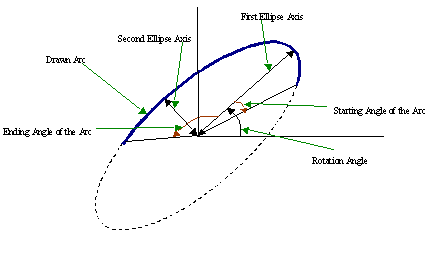
\includegraphics[width=0.5\textwidth]{pics/ellipse.png}

\cvfunc{ellipse2Poly}\label{ellipse2Poly}
Approximates an elliptic arc with a polyline

\begin{lstlisting}
void ellipse2Poly( Point center, Size axes, int angle,
                   int startAngle, int endAngle, int delta,
                   vector<Point>& pts );
\end{lstlisting}
\begin{description}
\cvarg{center}{Center of the arc}
\cvarg{axes}{Half-sizes of the arc. See \cross{ellipse}}
\cvarg{angle}{Rotation angle of the ellipse in degrees. See \cross{ellipse}}
\cvarg{startAngle}{Starting angle of the elliptic arc in degrees}
\cvarg{endAngle}{Ending angle of the elliptic arc in degrees}
\cvarg{delta}{Angle between the subsequent polyline vertices. It defines the approximation accuracy.}
\cvarg{pts}{The output vector of polyline vertices}
\end{description}

The function \texttt{ellipse2Poly} computes the vertices of a polyline that approximates the specified elliptic arc. It is used by \cross{ellipse}.

\cvfunc{fillConvexPoly}\label{fillConvexPoly}
Fills a convex polygon.

\begin{lstlisting}
void fillConvexPoly(Mat& img, const Point* pts, int npts,
                    const Scalar& color, int lineType=8,
                    int shift=0);
\end{lstlisting}
\begin{description}
\cvarg{img}{Image}
\cvarg{pts}{The polygon vertices}
\cvarg{npts}{The number of polygon vertices}
\cvarg{color}{Polygon color}
\cvarg{lineType}{Type of the polygon boundaries, see \cross{line} description}
\cvarg{shift}{The number of fractional bits in the vertex coordinates}
\end{description}

The function \texttt{fillConvexPoly} draws a filled convex polygon.
This function is much faster than the function \texttt{fillPoly}
and can fill not only convex polygons but any monotonic polygon without self-intersections,
i.e., a polygon whose contour intersects every horizontal line (scan
line) twice at the most (though, its top-most and/or the bottom edge could be horizontal).

\cvfunc{fillPoly}\label{fillPoly}
Fills the area bounded by one or more polygons

\begin{lstlisting}
void fillPoly(Mat& img, const Point** pts, const int* npts, int ncontours,
              const Scalar& color, int lineType=8, int shift=0,
              Point offset=Point() );
\end{lstlisting}
\begin{description}
\cvarg{img}{Image}
\cvarg{pts}{Array of polygons, each represented as an array of points}
\cvarg{npts}{The array of polygon vertex counters}
\cvarg{ncontours}{The number of contours that bind the filled region}
\cvarg{color}{Polygon color}
\cvarg{lineType}{Type of the polygon boundaries, see \cross{line} description}
\cvarg{shift}{The number of fractional bits in the vertex coordinates}
\end{description}

The function \texttt{fillPoly} fills an area bounded by several
polygonal contours. The function can fills complex areas, for example,
areas with holes, contours with self-intersections (some of thier parts), and so forth.

\cvfunc{getTextSize}\label{getTextSize}
Calculates the width and height of a text string.

\begin{lstlisting}
Size getTextSize(const string& text, int fontFace,
                 double fontScale, int thickness,
                 int* baseLine);
\end{lstlisting}
\begin{description}
\cvarg{text}{The input text string}
\cvarg{fontFace}{The font to use; see \cross{putText}}
\cvarg{fontScale}{The font scale; see \cross{putText}}
\cvarg{thickness}{The thickness of lines used to render the text; see \cross{putText}}
\cvarg{baseLine}{The output parameter - y-coordinate of the baseline relative to the bottom-most text point}
\end{description}

The function \texttt{getTextSize} calculates and returns size of the box that contain the specified text.
That is, the following code will render some text, the tight box surrounding it and the baseline:

\begin{lstlisting}
// Use "y" to show that the baseLine is about
string text = "Funny text inside the box";
int fontFace = FONT_HERSHEY_SCRIPT_SIMPLEX;
double fontScale = 2;
int thickness = 3;

Mat img(600, 800, CV_8UC3, Scalar::all(0));

int baseline=0;
Size textSize = getTextSize(text, fontFace,
                            fontScale, thickness, &baseline);
baseline += thickness;

// center the text
Point textOrg((img.cols - textSize.width)/2,
              (img.rows + textSize.height)/2);

// draw the box
rectangle(img, textOrg + Point(0, baseline),
          textOrg + Point(textSize.width, -textSize.height),
          Scalar(0,0,255));
// ... and the baseline first
line(img, textOrg + Point(0, thickness),
     textOrg + Point(textSize.width, thickness),
     Scalar(0, 0, 255));

// then put the text itself
putText(img, text, textOrg, fontFace, fontScale,
        Scalar::all(255), thickness, 8);
\end{lstlisting}
        
        
\cvfunc{line}\label{line}
Draws a line segment connecting two points

\begin{lstlisting}
void line(Mat& img, Point pt1, Point pt2, const Scalar& color,
          int thickness=1, int lineType=8, int shift=0);
\end{lstlisting}
\begin{description}
\cvarg{img}{The image}
\cvarg{pt1}{First point of the line segment}
\cvarg{pt2}{Second point of the line segment}
\cvarg{color}{Line color}
\cvarg{thickness}{Line thickness}
\cvarg{lineType}{Type of the line:
  \begin{description}
  \cvarg{8}{(or omitted) 8-connected line.}
  \cvarg{4}{4-connected line.}
  \cvarg{CV\_AA}{antialiased line.}
  \end{description}}
\cvarg{shift}{Number of fractional bits in the point coordinates}
\end{description}

The function \texttt{line} draws the line segment between
\texttt{pt1} and \texttt{pt2} points in the image. The line is
clipped by the image boundaries. For non-antialiased lines
with integer coordinates the 8-connected or 4-connected Bresenham
algorithm is used. Thick lines are drawn with rounding endings.
Antialiased lines are drawn using Gaussian filtering. To specify
the line color, the user may use the macro
\texttt{CV\_RGB(r, g, b)}.


\cvfunc{LineIterator}\label{LineIterator}
Class for iterating pixels on a raster line

\begin{lstlisting}
class LineIterator
{
public:
    // creates iterators for the line connecting pt1 and pt2
    // the line will be clipped on the image boundaries
    // the line is 8-connected or 4-connected
    // If leftToRight=true, then the iteration is always done
    // from the left-most point to the right most,
    // not to depend on the ordering of pt1 and pt2 parameters
    LineIterator(const Mat& img, Point pt1, Point pt2,
                 int connectivity=8, bool leftToRight=false);
    // returns pointer to the current line pixel
    uchar* operator *();
    // move the iterator to the next pixel
    LineIterator& operator ++();
    LineIterator operator ++(int);

    // internal state of the iterator
    uchar* ptr;
    int err, count;
    int minusDelta, plusDelta;
    int minusStep, plusStep;
};
\end{lstlisting}

The class \texttt{LineIterator} is used to get each pixel of a raster line. It can be treated as versatile implementation of the Bresenham algorithm, where you can stop at each pixel and do some extra processing, for example, grab pixel values along the line, or draw a line with some effect (e.g. with XOR operation).

The number of pixels along the line is store in \texttt{LineIterator::count}.

\begin{lstlisting}
\\ grabs pixels along the line (pt1, pt2)
\\ from 8-bit 3-channel image to the buffer
LineIterator it(img, pt1, pt2, 8);
vector<Vec3b> buf(it.count);

for(int i = 0; i < it.count; i++, ++it)
    buf[i] = *(const Vec3b)*it;
\end{lstlisting}


\cvfunc{rectangle}\label{rectangle}
Draws a simple, thick, or filled up-right rectangle.

\begin{lstlisting}
void rectangle(Mat& img, Point pt1, Point pt2,
               const Scalar& color, int thickness=1,
               int lineType=8, int shift=0);
\end{lstlisting}
\begin{description}
\cvarg{img}{Image}
\cvarg{pt1}{One of the rectangle's vertices}
\cvarg{pt2}{Opposite to \texttt{pt1} rectangle vertex}
\cvarg{color}{Rectangle color or brightness (grayscale image)}
\cvarg{thickness}{Thickness of lines that make up the rectangle. Negative values, e.g. \texttt{CV\_FILLED}, mean that the function has to draw a filled rectangle.}
\cvarg{lineType}{Type of the line, see \cross{line} description}
\cvarg{shift}{Number of fractional bits in the point coordinates}
\end{description}

The function \texttt{rectangle} draws a rectangle outline or a filled rectangle, which two opposite corners are \texttt{pt1} and \texttt{pt2}.
               

\cvfunc{polylines}\label{polylines}
Draws several polygonal curves

\begin{lstlisting}
void polylines(Mat& img, const Point** pts, const int* npts,
               int ncontours, bool isClosed, const Scalar& color,
               int thickness=1, int lineType=8, int shift=0 );
\end{lstlisting}
\begin{description}
\cvarg{img}{The image}
\cvarg{pts}{Array of polygonal curves}
\cvarg{npts}{Array of polygon vertex counters}
\cvarg{ncontours}{The number of curves}
\cvarg{isClosed}{Indicates whether the drawn polylines are closed or not. If they are closed, the function draws the line from the last vertex of each curve to its first vertex}
\cvarg{color}{Polyline color}
\cvarg{thickness}{Thickness of the polyline edges}
\cvarg{lineType}{Type of the line segments, see \cross{line} description}
\cvarg{shift}{The number of fractional bits in the vertex coordinates}
\end{description}

The function \texttt{polylines} draws one or more polygonal curves.

\cvfunc{putText}\label{putText}
Draws a text string

\begin{lstlisting}
void putText( Mat& img, const string& text, Point org,
              int fontFace, double fontScale, Scalar color,
              int thickness=1, int lineType=8,
              bool bottomLeftOrigin=false );
enum
{
 FONT_HERSHEY_SIMPLEX = 0,
 FONT_HERSHEY_PLAIN = 1,
 FONT_HERSHEY_DUPLEX = 2,
 FONT_HERSHEY_COMPLEX = 3,
 FONT_HERSHEY_TRIPLEX = 4,
 FONT_HERSHEY_COMPLEX_SMALL = 5,
 FONT_HERSHEY_SCRIPT_SIMPLEX = 6,
 FONT_HERSHEY_SCRIPT_COMPLEX = 7,
 FONT_ITALIC = 16
};
\end{lstlisting}
\begin{description}
\cvarg{img}{The image}
\cvarg{text}{The text string to be drawn}
\cvarg{org}{The bottom-left corner of the text string in the image}
\cvarg{fontFace}{The font type, one of \texttt{FONT\_HERSHEY\_...}}
\cvarg{fontScale}{The font scale factor that is multiplied by the font-specific base size}
\cvarg{thickness}{Thickness of the lines used to draw the text}
\cvarg{lineType}{The line type; see \texttt{line} for details}
\cvarg{bottomLeftOrigin}{When true, the image data origin is at the bottom-left corner, otherwise it's at the top-left corner}
\end{description}

The function \texttt{putText} draws a text string in the image.
Symbols that can not be rendered using the specified font are
replaced question marks. See \cross{getTextSize} for a text rendering code example.

\subsection{XML/YAML Persistence}

\cvfunc{FileStorage}\label{FileStorage}
The XML/YAML file storage class

\begin{lstlisting}
class FileStorage
{
public:
    enum { READ=0, WRITE=1, APPEND=2 };
    enum { UNDEFINED=0, VALUE_EXPECTED=1, NAME_EXPECTED=2, INSIDE_MAP=4 };
    // the default constructor
    FileStorage();
    // the constructor that opens the file for reading
    // (flags=FileStorage::READ) or writing (flags=FileStorage::WRITE)
    FileStorage(const string& filename, int flags);
    // wraps the already opened CvFileStorage*
    FileStorage(CvFileStorage* fs);
    // the destructor; closes the file if needed
    virtual ~FileStorage();

    // opens the specified file for reading (flags=FileStorage::READ)
    // or writing (flags=FileStorage::WRITE)
    virtual bool open(const string& filename, int flags);
    // checks if the storage is opened
    virtual bool isOpened() const;
    // closes the file
    virtual void release();

    // returns the first top-level node
    FileNode getFirstTopLevelNode() const;
    // returns the root file node
    // (it's the parent of the first top-level node)
    FileNode root(int streamidx=0) const;
    // returns the top-level node by name
    FileNode operator[](const string& nodename) const;
    FileNode operator[](const char* nodename) const;

    // returns the underlying CvFileStorage*
    CvFileStorage* operator *() { return fs; }
    const CvFileStorage* operator *() const { return fs; }
    
    // writes the certain number of elements of the specified format
    // (see DataType) without any headers
    void writeRaw( const string& fmt, const uchar* vec, size_t len );
    
    // writes an old-style object (CvMat, CvMatND etc.)
    void writeObj( const string& name, const void* obj );

    // returns the default object name from the filename
    // (used by cvSave() with the default object name etc.)
    static string getDefaultObjectName(const string& filename);

    Ptr<CvFileStorage> fs;
    string elname;
    vector<char> structs;
    int state;
};
\end{lstlisting}


\cvfunc{FileNode}\label{FileNode}
The XML/YAML file node class

\begin{lstlisting}
class CV_EXPORTS FileNode
{
public:
    enum { NONE=0, INT=1, REAL=2, FLOAT=REAL, STR=3,
        STRING=STR, REF=4, SEQ=5, MAP=6, TYPE_MASK=7,
        FLOW=8, USER=16, EMPTY=32, NAMED=64 };
    FileNode();
    FileNode(const CvFileStorage* fs, const CvFileNode* node);
    FileNode(const FileNode& node);
    FileNode operator[](const string& nodename) const;
    FileNode operator[](const char* nodename) const;
    FileNode operator[](int i) const;
    int type() const;
    int rawDataSize(const string& fmt) const;
    bool empty() const;
    bool isNone() const;
    bool isSeq() const;
    bool isMap() const;
    bool isInt() const;
    bool isReal() const;
    bool isString() const;
    bool isNamed() const;
    string name() const;
    size_t size() const;
    operator int() const;
    operator float() const;
    operator double() const;
    operator string() const;

    FileNodeIterator begin() const;
    FileNodeIterator end() const;

    void readRaw( const string& fmt, uchar* vec, size_t len ) const;
    void* readObj() const;

    // do not use wrapper pointer classes for better efficiency
    const CvFileStorage* fs;
    const CvFileNode* node;
};
\end{lstlisting}

\cvfunc{FileNodeIterator}\label{FileNodeIterator}
The XML/YAML file node iterator class

\begin{lstlisting}
class CV_EXPORTS FileNodeIterator
{
public:
    FileNodeIterator();
    FileNodeIterator(const CvFileStorage* fs,
        const CvFileNode* node, size_t ofs=0);
    FileNodeIterator(const FileNodeIterator& it);
    FileNode operator *() const;
    FileNode operator ->() const;

    FileNodeIterator& operator ++();
    FileNodeIterator operator ++(int);
    FileNodeIterator& operator --();
    FileNodeIterator operator --(int);
    FileNodeIterator& operator += (int);
    FileNodeIterator& operator -= (int);

    FileNodeIterator& readRaw( const string& fmt, uchar* vec,
                               size_t maxCount=(size_t)INT_MAX );

    const CvFileStorage* fs;
    const CvFileNode* container;
    CvSeqReader reader;
    size_t remaining;
};
\end{lstlisting}

\subsection{Clustering and Search in Multi-Dimensional Spaces}

\cvfunc{kmeans}\label{kmeans}

\begin{lstlisting}
double kmeans( const Mat& samples, int clusterCount, Mat& labels,
               TermCriteria termcrit, int attempts,
               int flags, Mat* centers );
enum { KMEANS_RANDOM_CENTERS=0,
       KMEANS_PP_CENTERS=2,
       KMEANS_USE_INITIAL_LABELS=1 };
\end{lstlisting}
\begin{description}
\cvarg{samples}{Floating-point matrix of input samples, one row per sample}
\cvarg{clusterCount}{The number of clusters to split the set by}
\cvarg{labels}{The input/output integer array that will store the cluster indices for every sample}
\cvarg{termcrit}{Specifies maximum number of iterations and/or accuracy (distance the centers can move by between subsequent iterations)}

\cvarg{attempts}{How many times the algorithm is executed using different initial labelings. The algorithm returns the labels that yield the best compactness (see the last function parameter)}
\cvarg{flags}{It can take the following values:
\begin{description}
\cvarg{KMEANS\_RANDOM\_CENTERS}{Random initial centers are selected in each attempt}
\cvarg{KMEANS\_PP\_CENTERS}{Use kmeans++ center initialization by Arthur and Vassilvitskii}
\cvarg{KMEANS\_USE\_INITIAL\_LABELS}{During the first (and possibly the only) attempt, the
function uses the user-supplied labels instaed of computing them from the initial centers. For the second and further attempts, the function will use the random or semi-random centers (use one of \texttt{KMEANS\_*\_CENTERS} flag to specify the exact method)}
\end{description}}
\cvarg{centers}{The output matrix of the cluster centers, one row per each cluster center}
\end{description}

The function \texttt{kmeans} implements a k-means algorithm that finds the
centers of \texttt{clusterCount} clusters and groups the input samples
around the clusters. On output, $\texttt{labels}_i$ contains a 0-based cluster index for
the sample stored in the $i^{th}$ row of the \texttt{samples} matrix.

The function returns the compactness measure, which is computed as
\[
\sum_i \|\texttt{samples}_i - \texttt{centers}_{\texttt{labels}_i}\|^2
\]
after every attempt; the best (minimum) value is chosen and the
corresponding labels and the compactness value are returned by the function.
Basically, the user can use only the core of the function, set the number of
attempts to 1, initialize labels each time using some custom algorithm and pass them with
\newline (\texttt{flags}=\texttt{KMEAN\_USE\_INITIAL\_LABELS}) flag, and then choose the best (most-compact) clustering.

\cvfunc{partition}\label{partition}
Splits an element set into equivalency classes.

\begin{lstlisting}
template<typename _Tp, class _EqPredicate> int
    partition( const vector<_Tp>& vec, vector<int>& labels,
               _EqPredicate predicate=_EqPredicate());
\end{lstlisting}
\begin{description}
\cvarg{vec}{The set of elements stored as a vector}
\cvarg{labels}{The output vector of labels; will contain as many elements as \texttt{vec}. Each label \texttt{labels[i]} is 0-based cluster index of \texttt{vec[i]}}
\cvarg{predicate}{The equivalence predicate (i.e. pointer to a boolean function of two arguments or an instance of the class that has the method \texttt{bool operator()(const \_Tp\& a, const \_Tp\& b)}. The predicate returns true when the elements are certainly if the same class, and false if they may or may not be in the same class}
\end{description}

The generic function \texttt{partition} implements an $O(N^2)$ algorithm for
splitting a set of $N$ elements into one or more equivalency classes, as described in \url{http://en.wikipedia.org/wiki/Disjoint-set_data_structure}. The function
returns the number of equivalency classes.


\subsection{Fast Aproximate Nearest Neighbor Search}

\def\urltilda{\kern -.05em\lower .7ex\hbox{\~{}}\kern .04em}

This section documents OpenCV's interface to the FLANN\footnote{http://people.cs.ubc.ca/\urltilda mariusm/flann} library. FLANN (Fast Library for Approximate Nearest Neighbors) is a library that
contains a collection of algorithms optimized for fast nearest neighbor search in large datasets and for high dimensional features. More 
information about FLANN can be found in \cite{muja_flann_2009}.

\cvfunc{flann::Index}\label{flann::Index}
The FLANN nearest neighbor index class.
\begin{lstlisting}
  namespace flann {

    class Index 
    {
    public:
	    Index(const Mat& features, const IndexParams& params);

	    void knnSearch(const vector<float>& query, 
			   vector<int>& indices, 
			   vector<float>& dists, 
			   int knn, 
			   const SearchParams& params);
	    void knnSearch(const Mat& queries, 
                           Mat& indices, 
                           Mat& dists, 
                           int knn, 
		           const SearchParams& params);

	    int radiusSearch(const vector<float>& query, 
			     vector<int>& indices, 
			     vector<float>& dists, 
			     float radius, 
			     const SearchParams& params);
	    int radiusSearch(const Mat& query, 
			     Mat& indices, 
			     Mat& dists, 
			     float radius, 
			     const SearchParams& params);

	    void save(std::string filename);

	    int veclen() const;

	    int size() const;
    };
  }
\end{lstlisting}

\cvfunc{flann::Index::Index}\label{flann::Index::Index}
Constructs a nearest neighbor search index for a given dataset.
\begin{lstlisting}
Index::Index(const Mat& features, const IndexParams& params);
\end{lstlisting}
\begin{description}
\cvarg{features}{ Matrix of type CV\_32F containing the features(points) to index. The size of the matrix is num\_features x feature\_dimensionality.}
\cvarg{params}{Structure containing the index parameters. The type of index that will be constructed depends on the type of this parameter.}
\end{description}

The possible parameter types are:

\begin {itemize}
 \item \texttt{LinearIndexParams} - When passing an object of this type, the index will perform a linear, brute-force search.
\begin{lstlisting}
  struct LinearIndexParams : public IndexParams 
  {
  };
\end{lstlisting}

 \item \texttt{KDTreeIndexParams} - When passing an object of this type the index constructed will consist of a set 
of randomized kd-trees which will be searched in parallel.
\begin{lstlisting}
  struct KDTreeIndexParams : public IndexParams 
  {
	KDTreeIndexParams( int trees = 4 );
  };
\end{lstlisting}
\begin{description}
\cvarg{trees}{The number of parallel kd-trees to use. Good values are in the range [1..16]}
\end{description}

 \item \texttt{KMeansIndexParams}  - When passing an object of this type the index constructed will be a hierarchical k-means tree. 
\begin{lstlisting}
  struct KMeansIndexParams : public IndexParams 
  {
	KMeansIndexParams( int branching = 32, 
			   int iterations = 11,
			   flann_centers_init_t centers_init = CENTERS_RANDOM, 
			   float cb_index = 0.2 );	
  };
\end{lstlisting}
\begin{description}
\cvarg{branching}{ The branching factor to use for the hierarchical k-means tree }
\cvarg{iterations}{ The maximum number of iterations to use in the k-means clustering 
		    stage when building the k-means tree. A value of -1 used here means
		    that the k-means clustering should be iterated until convergence}
\cvarg{centers\_init}{ The algorithm to use for selecting the initial
		  centers when performing a k-means clustering step. The possible values are
		  CENTERS\_RANDOM (picks the initial cluster centers randomly), CENTERS\_GONZALES (picks the
		  initial centers using Gonzales' algorithm) and CENTERS\_KMEANSPP (picks the initial
		centers using the algorithm suggested in \cite{arthur_kmeanspp_2007}) }
\cvarg{cb\_index} { This parameter (cluster boundary index) influences the
		  way exploration is performed in the hierarchical kmeans tree. When \texttt{cb\_index} is zero
		  the next kmeans domain to be explored is choosen to be the one with the closest center. 
		  A value greater then zero also takes into account the size of the domain.}
\end{description}

 \item \texttt{CompositeIndexParams} - When using a parameters object of this type the index created combines the randomized kd-trees 
	and the hierarchical k-means tree.
\begin{lstlisting}
  struct CompositeIndexParams : public IndexParams 
  {
	CompositeIndexParams( int trees = 4, 
			      int branching = 32, 
			      int iterations = 11,
			      flann_centers_init_t centers_init = CENTERS_RANDOM, 
			      float cb_index = 0.2 );
  };
\end{lstlisting}

 \item \texttt{AutotunedIndexParams} - When passing an object of this type the index created is automatically tuned to offer 
the best performance, by choosing the optimal index type (randomized kd-trees, hierarchical kmeans, linear) and parameters for the
dataset provided.
\begin{lstlisting}
  struct AutotunedIndexParams : public IndexParams 
  {
	AutotunedIndexParams( float target_precision = 0.9, 
			      float build_weight = 0.01,
			      float memory_weight = 0, 
			      float sample_fraction = 0.1 );
  };
\end{lstlisting}
\begin{description}
\cvarg{target\_precision}{ Is a number between 0 and 1 specifying the
percentage of the approximate nearest-neighbor searches that return the
exact nearest-neighbor. Using a higher value for this parameter gives
more accurate results, but the search takes longer. The optimum value
usually depends on the application. }

\cvarg{build\_weight}{ Specifies the importance of the
index build time raported to the nearest-neighbor search time. In some
applications it's acceptable for the index build step to take a long time
if the subsequent searches in the index can be performed very fast. In
other applications it's required that the index be build as fast as
possible even if that leads to slightly longer search times.}

\cvarg{memory\_weight} {Is used to specify the tradeoff between
time (index build time and search time) and memory used by the index. A
value less than 1 gives more importance to the time spent and a value
greater than 1 gives more importance to the memory usage.}

\cvarg{sample\_fraction} {Is a number between 0 and 1 indicating what fraction
of the dataset to use in the automatic parameter configuration algorithm. Running the 
algorithm on the full dataset gives the most accurate results, but for
very large datasets can take longer than desired. In such case using just a fraction of the
data helps speeding up this algorithm while still giving good approximations of the
optimum parameters.}
\end{description}

 \item \texttt{SavedIndexParams} - This object type is used for loading a previously saved index from the disk.
\begin{lstlisting}
  struct SavedIndexParams : public IndexParams {
	SavedIndexParams( std::string filename );
  };
\end{lstlisting}
\begin{description}
\cvarg{filename}{ The filename in which the index was saved. }
\end{description}
\end {itemize}


\cvfunc{flann::Index::knnSearch}\label{flann::Index::knnSearch}
Performs a K-nearest neighbor search for a given query point using the index.
\begin{lstlisting}
void Index::knnSearch(const vector<float>& query, 
		vector<int>& indices, 
		vector<float>& dists, 
		int knn, 
		const SearchParams& params);
\end{lstlisting}
\begin{description}
\cvarg{query}{The query point}
\cvarg{indices}{Vector that will contain the indices of the K-nearest neighbors found. It must have at least knn size.}
\cvarg{dists}{Vector that will contain the distances to the K-nearest neighbors found. It must have at least knn size.}
\cvarg{knn}{Number of nearest neighbors to search for.}
\cvarg{params}{Search parameters}
\begin{lstlisting}
  struct SearchParams {
	  SearchParams(int checks = 32);
  };
\end{lstlisting}
\begin{description}
\cvarg{checks}{ The number of times the tree(s) in the index should be recursively traversed. A
higher value for this parameter would give better search precision, but
also take more time. If automatic configuration was used when the
index was created, the number of checks required to achieve the specified
precision was also computed, in which case this parameter is ignored.}
\end{description}
\end{description}

\cvfunc{flann::Index::knnSearch}\label{flann::Index::knnSearch}
Performs a K-nearest neighbor search for multiple query points.
\begin{lstlisting}
void Index::knnSearch(const Mat& queries, 
		Mat& indices, 
		Mat& dists, 
		int knn, 
		const SearchParams& params);
\end{lstlisting}
\begin{description}
\cvarg{queries}{The query points, one per row}
\cvarg{indices}{Indices of the nearest neighbors found }
\cvarg{dists}{Distances to the nearest neighbors found}
\cvarg{knn}{Number of nearest neighbors to search for}
\cvarg{params}{Search parameters}
\end{description}


\cvfunc{flann::Index::radiusSearch}\label{flann::Index::radiusSearch}
Performs a radius nearest neighbor search for a given query point.
\begin{lstlisting}
int Index::radiusSearch(const vector<float>& query, 
		  vector<int>& indices, 
		  vector<float>& dists, 
		  float radius, 
		  const SearchParams& params);
\end{lstlisting}
\begin{description}
\cvarg{query}{The query point}
\cvarg{indices}{Vector that will contain the indices of the points found within the search radius in decreasing order of the distance to the query point. If the number of neighbors in the search radius is bigger than the size of this vector, the ones that don't fit in the vector are ignored. }
\cvarg{dists}{Vector that will contain the distances to the points found within the search radius}
\cvarg{radius}{The search radius}
\cvarg{params}{Search parameters}
\end{description}


\cvfunc{flann::Index::radiusSearch}\label{flann::Index::radiusSearch}
Performs a radius nearest neighbor search for multiple query points.
\begin{lstlisting}
int Index::radiusSearch(const Mat& query, 
		  Mat& indices, 
		  Mat& dists, 
		  float radius, 
		  const SearchParams& params);
\end{lstlisting}
\begin{description}
\cvarg{queries}{The query points, one per row}
\cvarg{indices}{Indices of the nearest neighbors found}
\cvarg{dists}{Distances to the nearest neighbors found}
\cvarg{radius}{The search radius}
\cvarg{params}{Search parameters}
\end{description}


\cvfunc{flann::Index::save}\label{flann::Index::save}
Saves the index to a file.
\begin{lstlisting}
void Index::save(std::string filename);
\end{lstlisting}
\begin{description}
\cvarg{filename}{The file to save the index to}
\end{description}


\cvfunc{flann::hierarchicalClustering}\label{flann::hierarchicalClustering}
Clusters the given points by constructing a hierarchical k-means tree and choosing a cut in the tree that minimizes the cluster's variance.
\begin{lstlisting}
int hierarchicalClustering(const Mat& features, Mat& centers,
                                      const KMeansIndexParams& params);
\end{lstlisting}
\begin{description}
\cvarg{features}{The points to be clustered}
\cvarg{centers}{The centers of the clusters obtained. The number of rows in this matrix represents the number of clusters desired, 
however, because of the way the cut in the hierarchical tree is choosen, the number of clusters computed will be
 the highest number of the form $(branching-1)*k+1$ that's lower than the number of clusters desired, where $branching$ is the tree's 
branching factor (see description of the KMeansIndexParams).  }
\cvarg{params}{Parameters used in the construction of the hierarchical k-means tree}
\end{description}
The function returns the number of clusters computed.



\subsection{Utility and System Functions and Macros}

\cvfunc{alignPtr}\label{alignPtr}
Aligns pointer to the specified number of bytes

\begin{lstlisting}
template<typename _Tp> _Tp* alignPtr(_Tp* ptr, int n=sizeof(_Tp));
\end{lstlisting}
\begin{description}
\cvarg{ptr}{The aligned pointer}
\cvarg{n}{The alignment size; must be a power of two}
\end{description}

The function returns the aligned pointer of the same type as the input pointer:
\[\texttt{(\_Tp*)(((size\_t)ptr + n-1) \& -n)}\]


\cvfunc{alignSize}\label{alignSize}
Aligns a buffer size to the specified number of bytes

\begin{lstlisting}
size_t alignSize(size_t sz, int n);
\end{lstlisting}
\begin{description}
\cvarg{sz}{The buffer size to align}
\cvarg{n}{The alignment size; must be a power of two}
\end{description}

The function returns the minimum number that is greater or equal to \texttt{sz} and is divisble by \texttt{n}:
\[\texttt{(sz + n-1) \& -n}\]


\cvfunc{allocate}\label{allocate}
Allocates an array of elements

\begin{lstlisting}
template<typename _Tp> _Tp* allocate(size_t n);
\end{lstlisting}
\begin{description}
\cvarg{n}{The number of elements to allocate}
\end{description}

The generic function \texttt{allocate} allocates buffer for the specified number of elements. For each element the default constructor is called.


\cvfunc{allocate}\label{allocate}
Allocates an array of elements

\begin{lstlisting}
template<typename _Tp> void deallocate(_Tp* ptr, size_t n);
\end{lstlisting}
\begin{description}
\cvarg{ptr}{Pointer to the deallocated buffer}
\cvarg{n}{The number of elements in the buffer}
\end{description}

The generic function \texttt{deallocate} deallocates the buffer allocated with \cross{allocate}. The number of elements must match the number passed to \cross{allocate}.

\cvfunc{CV\_Assert}\label{CV Assert}
Checks a condition at runtime.

\begin{lstlisting}
#define CV_Assert( expr ) ...
#define CV_DbgAssert(expr) ...
\end{lstlisting}

\begin{description}
\cvarg{expr}{The checked expression}
\end{description}

The macros \texttt{CV\_Assert} and \texttt{CV\_DbgAssert} evaluate the specified expression and if it is 0, the macros raise an error (see \cross{error}). The macro \texttt{CV\_Assert} checks the condition in both Debug and Release configurations, while \texttt{CV\_DbgAssert} is only retained in the Debug configuration.

\cvfunc{error}\label{error}
Signals an error and raises the exception

\begin{lstlisting}
void error( const Exception& exc );

#define CV_Error( code, msg )
#define CV_Error_( code, args )
\end{lstlisting}
\begin{description}
\cvarg{exc}{The exception to throw}
\cvarg{code}{The error code, normally, a negative value. The list of pre-defined error codes can be found in \texttt{cxerror.h}}
\cvarg{msg}{Text of the error message}
\cvarg{args}{printf-like formatted error message in parantheses}
\end{description}

The function \texttt{error} and the helper macros \texttt{CV\_Error} and \texttt{CV\_Error\_} call the error handler. Currently, the error handler prints the error code (\texttt{exc.code}), the context (\texttt{exc.file}, \texttt{exc.line} and the error message \texttt{exc.err} to the standard error stream \texttt{stderr}. In Debug configuration it then provokes memory access violation, so that the execution stack and all the parameters can be analyzed in debugger. In Release configuration the exception \texttt{exc} is thrown.

The macro \texttt{CV\_Error\_} can be used to construct the error message on-fly to include some dynamic information, for example:

\begin{lstlisting}
// note the extra parentheses around the formatted text message
CV_Error_(CV_StsOutOfRange,
    ("the matrix element (%d,%d)=%g is out of range",
    i, j, mtx.at<float>(i,j)))
\end{lstlisting}


\cvfunc{Exception}\label{Exception}
The exception class passed to error

\begin{lstlisting}
class  Exception
{
public:
    // various constructors and the copy operation
    Exception() { code = 0; line = 0; }
    Exception(int _code, const string& _err,
              const string& _func, const string& _file, int _line);
    Exception(const Exception& exc);
    Exception& operator = (const Exception& exc);

    // the error code
    int code;
    // the error text message
    string err;
    // function name where the error happened
    string func;
    // the source file name where the error happened
    string file;
    // the source file line where the error happened
    int line;
};
\end{lstlisting}

The class \texttt{Exception} encapsulates all or almost all the necessary information about the error happened in the program. The exception is usually constructed and thrown implicitly, via \texttt{CV\_Error} and \texttt{CV\_Error\_} macros, see \cross{error}.


\cvfunc{fastMalloc}\label{fastMalloc}
Allocates aligned memory buffer

\begin{lstlisting}
void* fastMalloc(size_t size);
\end{lstlisting}
\begin{description}
\cvarg{size}{The allocated buffer size}
\end{description}
 
The function \texttt{fastMalloc} allocates buffer of the specified size and returns it. When the buffer size is 16 bytes or more, the returned buffer is aligned on 16 bytes.

\cvfunc{fastFree}\label{fastFree}
Deallocates memory buffer

\begin{lstlisting}
void fastFree(void* ptr);
\end{lstlisting}
\begin{description}
\cvarg{ptr}{Pointer to the allocated buffer}
\end{description}

The function \texttt{fastFree} deallocates the buffer, allocated with \cross{fastMalloc}.
If NULL pointer is passed, the function does nothing.

\cvfunc{format}\label{format}
Returns a text string formatted using printf-like expression

\begin{lstlisting}
string format( const char* fmt, ... );
\end{lstlisting}
\begin{description}
\cvarg{fmt}{The printf-compatible formatting specifiers}
\end{description}

The function \texttt{format} acts like \texttt{sprintf}, but forms and returns STL string. It can be used for form the error message in \cross{Exception} constructor.

\cvfunc{getNumThreads}\label{getNumThreads}
Returns the number of threads used by OpenCV

\begin{lstlisting}
int getNumThreads();
\end{lstlisting}

The function returns the number of threads that is used by OpenCV.

See also: \cross{setNumThreads}, \cross{getThreadNum}.


\cvfunc{getThreadNum}\label{getThreadNum}
Returns index of the currently executed thread

\begin{lstlisting}
int getThreadNum();
\end{lstlisting}

The function returns 0-based index of the currently executed thread. The function is only valid inside a parallel OpenMP region. When OpenCV is built without OpenMP support, the function always returns 0.

See also: \cross{setNumThreads}, \cross{getNumThreads}.

\cvfunc{getTickCount}\label{getTickCount}
Returns the number of ticks

\begin{lstlisting}
int64 getTickCount();
\end{lstlisting}

The function returns the number of ticks since the certain event (e.g. when the machine was turned on).
It can be used to initialize \cross{RNG} or to measure a function execution time by reading the tick count before and after the function call. See also the tick frequency.

\cvfunc{getTickFrequency}\label{getTickFrequency}
Returns the number of ticks per second

\begin{lstlisting}
double getTickFrequency();
\end{lstlisting}

The function returns the number of ticks per second.
That is, the following code computes the executing time in seconds.
\begin{lstlisting}
double t = (double)getTickCount();
// do something ...
t = ((double)getTickCount() - t)/getTickFrequency();
\end{lstlisting}

\cvfunc{setNumThreads}\label{setNumThreads}
Sets the number of threads used by OpenCV

\begin{lstlisting}
void setNumThreads(int nthreads);
\end{lstlisting}
\begin{description}
\cvarg{nthreads}{The number of threads used by OpenCV}
\end{description}

The function sets the number of threads used by OpenCV in parallel OpenMP regions. If \texttt{nthreads=0}, the function will use the default number of threads, which is usually equal to the number of the processing cores.

See also: \cross{getNumThreads}, \cross{getThreadNum}

\section{CV. Image Processing and Computer Vision}

\subsection{Image Filtering}

\cvfunc{BaseColumnFilter}\label{BaseColumnFilter}
Base class for filters with single-column kernels

\begin{lstlisting}
class BaseColumnFilter
{
public:
    virtual ~BaseColumnFilter();
    // runs filtering operation on the set of rows,
    // "dstcount + ksize - 1" rows on input,
    // "dstcount" rows on output,
    // each input and output row has "width" elements
    // the filtered rows are written into "dst" buffer.
    virtual void operator()(const uchar** src, uchar* dst, int dststep,
                            int dstcount, int width) = 0;
    // resets the filter state (may be needed for IIR filters)
    virtual void reset();
    
    int ksize; // the aperture size
    int anchor; // position of the anchor point,
                // normally not used during the processing
};
\end{lstlisting}

The class \texttt{BaseColumnFilter} is the base class for filtering data using single-column kernels. The filtering does not have to be a linear operation. In general, it could be written as following:

\[\texttt{dst}(x,y) = F(\texttt{src}[y](x), \texttt{src}[y+1](x), ..., \texttt{src}[y+\texttt{ksize}-1](x)\]

where $F$ is the filtering function, but, as it is represented as a class, it can produce any side effects, memorize previously processed data etc. The class only defines the interface and is not used directly. Instead, there are several functions in OpenCV (and you can add more) that return pointers to the derived classes that implement specific filtering operations. Those pointers are then passed to \cross{FilterEngine} constructor. While the filtering operation interface uses \texttt{uchar} type, a particular implementation is not limited to 8-bit data.

See also: \cross{BaseRowFilter}, \cross{BaseFilter}, \cross{FilterEngine},
    \cross{getColumnSumFilter}, \cross{getLinearColumnFilter}, \cross{getMorphologyColumnFilter}


\cvfunc{BaseFilter}\label{BaseFilter}
Base class for 2D image filters

\begin{lstlisting}
class BaseFilter
{
public:
    virtual ~BaseFilter();
    // runs filtering operation on the set of rows,
    // "dstcount + ksize.height - 1" rows on input,
    // "dstcount" rows on output,
    // each input row has "(width + ksize.width-1)*cn" elements
    // each output row has "width*cn" elements.
    // the filtered rows are written into "dst" buffer.
    virtual void operator()(const uchar** src, uchar* dst, int dststep,
                            int dstcount, int width, int cn) = 0;
    // resets the filter state (may be needed for IIR filters)                        
    virtual void reset();
    Size ksize;
    Point anchor;
};
\end{lstlisting}

The class \texttt{BaseFilter} is the base class for filtering data using 2D kernels. The filtering does not have to be a linear operation. In general, it could be written as following:

\[
  \begin{array}{l}
  \texttt{dst}(x,y) = F( \\
  \texttt{src}[y](x), \texttt{src}[y](x+1), ..., \texttt{src}[y](x+\texttt{ksize.width}-1), \\
  \texttt{src}[y+1](x), \texttt{src}[y+1](x+1), ..., \texttt{src}[y+1](x+\texttt{ksize.width}-1), \\
  ......................................................................................... \\
  \texttt{src}[y+\texttt{ksize.height-1}](x), \texttt{src}[y+\texttt{ksize.height-1}](x+1), ..., \texttt{src}[y+\texttt{ksize.height-1}](x+\texttt{ksize.width}-1))
  \end{array}
  \]

where $F$ is the filtering function. The class only defines the interface and is not used directly. Instead, there are several functions in OpenCV (and you can add more) that return pointers to the derived classes that implement specific filtering operations. Those pointers are then passed to \cross{FilterEngine} constructor. While the filtering operation interface uses \texttt{uchar} type, a particular implementation is not limited to 8-bit data.

See also: \cross{BaseColumnFilter}, \cross{BaseRowFilter}, \cross{FilterEngine},
    \cross{getLinearFilter}, \cross{getMorphologyFilter}

\cvfunc{BaseRowFilter}\label{BaseRowFilter}
Base class for filters with single-row kernels

\begin{lstlisting}
class BaseRowFilter
{
public:
    virtual ~BaseRowFilter();
    
    virtual void operator()(const uchar* src, uchar* dst,
                            int width, int cn) = 0;
    int ksize, anchor;
};
\end{lstlisting}

The class \texttt{BaseRowFilter} is the base class for filtering data using single-row kernels. The filtering does not have to be a linear operation. In general, it could be written as following:

\[\texttt{dst}(x,y) = F(\texttt{src}[y](x), \texttt{src}[y](x+1), ..., \texttt{src}[y](x+\texttt{ksize.width}-1))\]

where $F$ is the filtering function. The class only defines the interface and is not used directly. Instead, there are several functions in OpenCV (and you can add more) that return pointers to the derived classes that implement specific filtering operations. Those pointers are then passed to \cross{FilterEngine} constructor. While the filtering operation interface uses \texttt{uchar} type, a particular implementation is not limited to 8-bit data.

See also: \cross{BaseColumnFilter}, \cross{Filter}, \cross{FilterEngine},
 \cross{getLinearRowFilter}, \cross{getMorphologyRowFilter}, \cross{getRowSumFilter}

\cvfunc{FilterEngine}\label{FilterEngine}
Generic image filtering class

\begin{lstlisting}
class FilterEngine
{
public:
    // empty constructor
    FilterEngine();
    // builds a 2D non-separable filter (!_filter2D.empty()) or
    // a separable filter (!_rowFilter.empty() && !_columnFilter.empty())
    // the input data type will be "srcType", the output data type will be "dstType",
    // the intermediate data type is "bufType".
    // _rowBorderType and _columnBorderType determine how the image
    // will be extrapolated beyond the image boundaries.
    // _borderValue is only used when _rowBorderType and/or _columnBorderType
    // == cv::BORDER_CONSTANT
    FilterEngine(const Ptr<BaseFilter>& _filter2D,
                 const Ptr<BaseRowFilter>& _rowFilter,
                 const Ptr<BaseColumnFilter>& _columnFilter,
                 int srcType, int dstType, int bufType,
                 int _rowBorderType=BORDER_REPLICATE,
                 int _columnBorderType=-1, // use _rowBorderType by default 
                 const Scalar& _borderValue=Scalar());
    virtual ~FilterEngine();
    // separate function for the engine initialization
    void init(const Ptr<BaseFilter>& _filter2D,
              const Ptr<BaseRowFilter>& _rowFilter,
              const Ptr<BaseColumnFilter>& _columnFilter,
              int srcType, int dstType, int bufType,
              int _rowBorderType=BORDER_REPLICATE, int _columnBorderType=-1,
              const Scalar& _borderValue=Scalar());
    // starts filtering of the ROI in an image of size "wholeSize".
    // returns the starting y-position in the source image.
    virtual int start(Size wholeSize, Rect roi, int maxBufRows=-1);
    // alternative form of start that takes the image
    // itself instead of "wholeSize". Set isolated to true to pretend that
    // there are no real pixels outside of the ROI
    // (so that the pixels will be extrapolated using the specified border modes)
    virtual int start(const Mat& src, const Rect& srcRoi=Rect(0,0,-1,-1),
                      bool isolated=false, int maxBufRows=-1);
    // processes the next portion of the source image,
    // "srcCount" rows starting from "src" and
    // stores the results to "dst".
    // returns the number of produced rows
    virtual int proceed(const uchar* src, int srcStep, int srcCount,
                        uchar* dst, int dstStep);
    // higher-level function that processes the whole
    // ROI or the whole image with a single call
    virtual void apply( const Mat& src, Mat& dst,
                        const Rect& srcRoi=Rect(0,0,-1,-1),
                        Point dstOfs=Point(0,0),
                        bool isolated=false);
    bool isSeparable() const { return filter2D.empty(); }
    // how many rows from the input image are not yet processed
    int remainingInputRows() const;
    // how many output rows are not yet produced
    int remainingOutputRows() const;
    ...
    // the starting and the ending rows in the source image
    int startY, endY;
    
    // pointers to the filters
    Ptr<BaseFilter> filter2D;
    Ptr<BaseRowFilter> rowFilter;
    Ptr<BaseColumnFilter> columnFilter;
};
\end{lstlisting}

The class \texttt{FilterEngine} can be used to apply an arbitrary filtering operation to an image.
It contains all the necessary intermediate buffers, it computes extrapolated values
of the "virtual" pixels outside of the image etc. Pointers to the initialized \texttt{FilterEngine} instances
are returned by various \texttt{create*Filter} functions, see below, and they are used inside high-level functions such as \cross{filter2D}, \cross{erode}, \cross{dilate} etc, that is, the class is the workhorse in many of OpenCV filtering functions.

This class makes it easier (though, maybe not very easy yet) to combine filtering operations with other operations, such as color space conversions, thresholding, arithmetic operations, etc. By combining several operations together you can get much better performance because your data will stay in cache. For example, below is the implementation of Laplace operator for a floating-point images, which is a simplified implementation of \cross{Laplacian}:

\begin{lstlisting}
void laplace_f(const Mat& src, Mat& dst)
{
    CV_Assert( src.type() == CV_32F );
    dst.create(src.size(), src.type());
    
    // get the derivative and smooth kernels for d2I/dx2.
    // for d2I/dy2 we could use the same kernels, just swapped
    Mat kd, ks;
    getSobelKernels( kd, ks, 2, 0, ksize, false, ktype );
    
    // let's process 10 source rows at once
    int DELTA = std::min(10, src.rows);
    Ptr<FilterEngine> Fxx = createSeparableLinearFilter(src.type(),
        dst.type(), kd, ks, Point(-1,-1), 0, borderType, borderType, Scalar() ); 
    Ptr<FilterEngine> Fyy = createSeparableLinearFilter(src.type(),
        dst.type(), ks, kd, Point(-1,-1), 0, borderType, borderType, Scalar() );

    int y = Fxx->start(src), dsty = 0, dy = 0;
    Fyy->start(src);
    const uchar* sptr = src.data + y*src.step;

    // allocate the buffers for the spatial image derivatives;
    // the buffers need to have more than DELTA rows, because at the
    // last iteration the output may take max(kd.rows-1,ks.rows-1)
    // rows more than the input.
    Mat Ixx( DELTA + kd.rows - 1, src.cols, dst.type() );
    Mat Iyy( DELTA + kd.rows - 1, src.cols, dst.type() );
    
    // inside the loop we always pass DELTA rows to the filter
    // (note that the "proceed" method takes care of possibe overflow, since
    // it was given the actual image height in the "start" method)
    // on output we can get:
    //  * < DELTA rows (the initial buffer accumulation stage)
    //  * = DELTA rows (settled state in the middle)
    //  * > DELTA rows (then the input image is over, but we generate
    //                  "virtual" rows using the border mode and filter them)
    // this variable number of output rows is dy.
    // dsty is the current output row.
    // sptr is the pointer to the first input row in the portion to process
    for( ; dsty < dst.rows; sptr += DELTA*src.step, dsty += dy )
    {
        Fxx->proceed( sptr, (int)src.step, DELTA, Ixx.data, (int)Ixx.step );
        dy = Fyy->proceed( sptr, (int)src.step, DELTA, d2y.data, (int)Iyy.step );
        if( dy > 0 )
        {
            Mat dstripe = dst.rowRange(dsty, dsty + dy);
            add(Ixx.rowRange(0, dy), Iyy.rowRange(0, dy), dstripe);
        }
    }
}
\end{lstlisting}

If you do not need that much control of the filtering process, you can simply use the \texttt{FilterEngine::apply} method. Here is how the method is actually implemented:

\begin{lstlisting}
void FilterEngine::apply(const Mat& src, Mat& dst,
    const Rect& srcRoi, Point dstOfs, bool isolated)
{
    // check matrix types
    CV_Assert( src.type() == srcType && dst.type() == dstType );
    
    // handle the "whole image" case
    Rect _srcRoi = srcRoi;
    if( _srcRoi == Rect(0,0,-1,-1) )
        _srcRoi = Rect(0,0,src.cols,src.rows);
    
    // check if the destination ROI is inside the dst.
    // and FilterEngine::start will check if the source ROI is inside src.
    CV_Assert( dstOfs.x >= 0 && dstOfs.y >= 0 &&
        dstOfs.x + _srcRoi.width <= dst.cols &&
        dstOfs.y + _srcRoi.height <= dst.rows );

    // start filtering
    int y = start(src, _srcRoi, isolated);
    
    // process the whole ROI. Note that "endY - startY" is the total number
    // of the source rows to process
    // (including the possible rows outside of srcRoi but inside the source image)
    proceed( src.data + y*src.step,
             (int)src.step, endY - startY,
             dst.data + dstOfs.y*dst.step +
             dstOfs.x*dst.elemSize(), (int)dst.step );
}
\end{lstlisting}

Unlike the earlier versions of OpenCV, now the filtering operations fully support the notion of image ROI, that is, pixels outside of the ROI but inside the image can be used in the filtering operations. For example, you can take a ROI of a single pixel and filter it - that will be a filter response at that particular pixel (however, it's possible to emulate the old behavior by passing \texttt{isolated=false} to \texttt{FilterEngine::start} or \texttt{FilterEngine::apply}). You can pass the ROI explicitly to \texttt{FilterEngine::apply}, or construct a new matrix headers:

\begin{lstlisting}
// compute dI/dx derivative at src(x,y)

// method 1:
// form a matrix header for a single value
float val1 = 0;
Mat dst1(1,1,CV_32F,&val1);

Ptr<FilterEngine> Fx = createDerivFilter(CV_32F, CV_32F,
                        1, 0, 3, BORDER_REFLECT_101);
Fx->apply(src, Rect(x,y,1,1), Point(), dst1);

// method 2:
// form a matrix header for a single value
float val2 = 0;
Mat dst2(1,1,CV_32F,&val2);

Mat pix_roi(src, Rect(x,y,1,1));
Sobel(pix_roi, dst2, dst2.type(), 1, 0, 3, 1, 0, BORDER_REFLECT_101);

printf("method1 = %g, method2 = %g\n", val1, val2);
\end{lstlisting}

Note on the data types. As it was mentioned in \cross{BaseFilter} description, the specific filters can process data of any type, despite that \texttt{Base*Filter::operator()} only takes \texttt{uchar} pointers and no information about the actual types. To make it all work, the following rules are used:

\begin{itemize}
    \item in case of separable filtering \texttt{FilterEngine::rowFilter} applied first. It transforms the input image data (of type \texttt{srcType}) to the intermediate results stored in the internal buffers (of type \texttt{bufType}). Then these intermediate results are processed \emph{as single-channel data} with \texttt{FilterEngine::columnFilter} and stored in the output image (of type \texttt{dstType}). Thus, the input type for \texttt{rowFilter} is \texttt{srcType} and the output type is \texttt{bufType}; the input type for \texttt{columnFilter} is \texttt{CV\_MAT\_DEPTH(bufType)} and the output type is \texttt{CV\_MAT\_DEPTH(dstType)}.
    
    \item in case of non-separable filtering \texttt{bufType} must be the same as \texttt{srcType}. The source data is copied to the temporary buffer if needed and then just passed to \texttt{FilterEngine::filter2D}. That is, the input type for \texttt{filter2D} is \texttt{srcType} (=\texttt{bufType}) and the output type is \texttt{dstType}.
\end{itemize}

See also: \cross{BaseColumnFilter}, \cross{BaseFilter}, \cross{BaseRowFilter}, \cross{createBoxFilter},
\cross{createDerivFilter}, \cross{createGaussianFilter}, \cross{createLinearFilter},
\cross{createMorphologyFilter}, \cross{createSeparableLinearFilter}

\cvfunc{bilateralFilter}\label{bilateralFilter}
Applies bilateral filter to the image

\begin{lstlisting}
void bilateralFilter( const Mat& src, Mat& dst, int d,
                      double sigmaColor, double sigmaSpace,
                      int borderType=BORDER_DEFAULT );
\end{lstlisting}
\begin{description}
\cvarg{src}{The source 8-bit or floating-point, 1-channel or 3-channel image}
\cvarg{dst}{The destination image; will have the same size and the same type as \texttt{src}}
\cvarg{d}{The diameter of each pixel neighborhood, that is used during filtering. If it is non-positive, it's computed from \texttt{sigmaSpace}}
\cvarg{sigmaColor}{Filter sigma in the color space. Larger value of the parameter means that farther colors within the pixel neighborhood (see \texttt{sigmaSpace}) will be mixed together, resulting in larger areas of semi-equal color}
\cvarg{sigmaSpace}{Filter sigma in the coordinate space. Larger value of the parameter means that farther pixels will influence each other (as long as their colors are close enough; see \texttt{sigmaColor}). Then \texttt{d>0}, it specifies the neighborhood size regardless of \texttt{sigmaSpace}, otherwise \texttt{d} is proportional to \texttt{sigmaSpace}}
\end{description}

The function applies bilateral filtering to the input image, as described in
\url{http://www.dai.ed.ac.uk/CVonline/LOCAL\_COPIES/MANDUCHI1/Bilateral\_Filtering.html}

\cvfunc{blur}\label{blur}
Smoothes image using normalized box filter

\begin{lstlisting}
void blur( const Mat& src, Mat& dst,
           Size ksize, Point anchor=Point(-1,-1),
           int borderType=BORDER_DEFAULT );
\end{lstlisting}
\begin{description}
\cvarg{src}{The source image}
\cvarg{dst}{The destination image; will have the same size and the same type as \texttt{src}}
\cvarg{ksize}{The smoothing kernel size}
\cvarg{anchor}{The anchor point. The default value \texttt{Point(-1,-1)} means that the anchor is at the kernel center}
\cvarg{borderType}{The border mode used to extrapolate pixels outside of the image}
\end{description}

The function \texttt{blur} smoothes the image using the kernel:

\[ \texttt{K} = \frac{1}{\texttt{ksize.width*ksize.height}}
\begin{bmatrix}
1 1 1 ... 1 1 \\
1 1 1 ... 1 1 \\
............... \\
1 1 1 ... 1 1
\end{bmatrix}
\]

The call \texttt{blur(src, dst, ksize, anchor, borderType)} is equivalent to
\texttt{boxFilter(src, dst, src.type(), anchor, true, borderType)}.

See also: \cross{boxFilter}, \cross{bilateralFilter}, \cross{GaussianBlur}, \cross{medianBlur}.

\cvfunc{borderInterpolate}\label{borderInterpolate}
Computes source location of extrapolated pixel

\begin{lstlisting}
int borderInterpolate( int p, int len, int borderType );

enum { // the first and the last pixels in each row and each column are replicated
       BORDER_REPLICATE=IPL_BORDER_REPLICATE,
       // 
       BORDER_CONSTANT=IPL_BORDER_CONSTANT,
       BORDER_REFLECT=IPL_BORDER_REFLECT,
       BORDER_REFLECT_101=IPL_BORDER_REFLECT_101,
       BORDER_REFLECT101=BORDER_REFLECT_101,
       BORDER_WRAP=IPL_BORDER_WRAP,
       BORDER_TRANSPARENT,
       BORDER_DEFAULT=BORDER_REFLECT_101,
       BORDER_ISOLATED=16 };
\end{lstlisting}
\begin{description}
\cvarg{p}{0-based coordinate of the extrapolated pixel along one of the axes, likely <0 or >=\texttt{len}}
\cvarg{len}{length of the array along the corresponding axis}
\cvarg{borderType}{the border type, one of the \texttt{BORDER\_*}, except for \texttt{BORDER\_TRANSPARENT} and \texttt{BORDER\_ISOLATED}. When \texttt{borderType==BORDER\_CONSTANT} the function always returns -1, regardless of \texttt{p} and \texttt{len}}
\end{description}

The function computes and returns the coordinate of the donor pixel, corresponding to the specified extrapolated pixel when using the specified extrapolation border mode. For example, if we use \texttt{BORDER\_WRAP} mode in the horizontal direction, \texttt{BORDER\_REFLECT\_101} in the vertical direction and want to compute value of the "virtual" pixel \texttt{Point(-5, 100)} in a floating-point image \texttt{img}, it will be

\begin{lstlisting}
float val = img.at<float>(borderInterpolate(100, img.rows, BORDER_REFLECT_101),
                          borderInterpolate(-5, img.cols, BORDER_WRAP));
\end{lstlisting}

Normally, the function is not called directly; it is used inside \cross{FilterEngine} and \cross{copyMakeBorder} to compute tables for quick extrapolation.

See also: \cross{FilterEngine}, \cross{copyMakeBorder}

\cvfunc{boxFilter}\label{boxFilter}
Smoothes image using box filter

\begin{lstlisting}
void boxFilter( const Mat& src, Mat& dst, int ddepth,
                Size ksize, Point anchor=Point(-1,-1),
                bool normalize=true,
                int borderType=BORDER_DEFAULT );
\end{lstlisting}
\begin{description}
\cvarg{src}{The source image}
\cvarg{dst}{The destination image; will have the same size and the same type as \texttt{src}}
\cvarg{ksize}{The smoothing kernel size}
\cvarg{anchor}{The anchor point. The default value \texttt{Point(-1,-1)} means that the anchor is at the kernel center}
\cvarg{normalize}{Indicates, whether the kernel is normalized by its area or not}
\cvarg{borderType}{The border mode used to extrapolate pixels outside of the image}
\end{description}

The function \texttt{boxFilter} smoothes the image using the kernel:

\[ \texttt{K} = \alpha
\begin{bmatrix}
1 & 1 & 1 & ... & 1 & 1 \\
1 & 1 & 1 & ... & 1 & 1 \\
\hdotsfor{6} \\
1 & 1 & 1 & ... & 1 & 1
\end{bmatrix}
\]

where

\[\alpha=\fork
{\frac{1}{\texttt{ksize.width*ksize.height}}}{when \texttt{normalize=true}}
{1}{otherwise} \]

Unnormalized box filter is useful for computing various integral characteristics over each pixel neighborhood, such as covariation matrices of image derivatives (used in dense optical flow algorithms, \href{conerHarris}{Harris corner detector} etc.). If you need to compute pixel sums over variable-size windows, use \cross{integral}.

See also: \cross{boxFilter}, \cross{bilateralFilter}, \cross{GaussianBlur}, \cross{medianBlur}, \cross{integral}.

\cvfunc{buildPyramid}\label{buildPyramid}
Constructs Gaussian pyramid for an image

\begin{lstlisting}
void buildPyramid( const Mat& src, vector<Mat>& dst, int maxlevel );
\end{lstlisting}
\begin{description}
\cvarg{src}{The source image; check \cross{pyrDown} for the list of supported types}
\cvarg{dst}{The destination vector of \texttt{maxlevel+1} images of the same type as \texttt{src};
\texttt{dst[0]} will be the same as \texttt{src}, \texttt{dst[1]} is the next pyramid layer,
a smoothed and down-sized \texttt{src} etc.}
\cvarg{maxlevel}{The 0-based index of the last (i.e. the smallest) pyramid layer; it must be non-negative}
\end{description}

The function \texttt{buildPyramid} constructs a vector of images and builds the gaussian pyramid by recursively applying \cross{pyrDown} to the previously built pyramid layers, starting from \texttt{dst[0]==src}.

\cvfunc{copyMakeBorder}\label{copyMakeBorder}
Forms a border around the image

\begin{lstlisting}
void copyMakeBorder( const Mat& src, Mat& dst,
                    int top, int bottom, int left, int right,
                    int borderType, const Scalar& value=Scalar() );
\end{lstlisting}
\begin{description}
\cvarg{src}{The source image}
\cvarg{dst}{The destination image; will have the same type as \texttt{src} and the size \texttt{Size(src.cols+left+right, src.rows+top+bottom)}}
\cvarg{top, bottom, left, right}{Specify how much pixels in each direction from the source image rectangle one needs to extrapolate, e.g. \texttt{top=1, bottom=1, left=1, right=1} mean that 1 pixel-wide border needs to be built}
\cvarg{borderType}{The border type; see \cross{borderInterpolate}}
\cvarg{value}{The border value if \texttt{borderType==BORDER\_CONSTANT}}
\end{description}

The function \texttt{copyMakeBorder} copies the source image into the middle of the destination image. The areas to the left, to the right, above and below the copied source image will be filled with extrapolated pixels. This is not what \cross{FilterEngine} or based on it filtering functions do (they extrapolate pixels on-fly), but what other more complex functions, including your own, may do to simplify image boundary handling.

The function supports the mode when \texttt{src} is already in the middle of \texttt{dst}. In this case the function does not copy \texttt{src} itself, but simply constructs the border, e.g.:

\begin{lstlisting}
// let border be the same in all directions
int border=2;
// constructs a larger image to fit both the image and the border
Mat gray_buf(rgb.rows + border*2, rgb.cols + border*2, rgb.depth());
// select the middle part of it w/o copying data
Mat gray(gray_canvas, Rect(border, border, rgb.cols, rgb.rows));
// convert image from RGB to grayscale
cvtColor(rgb, gray, CV_RGB2GRAY);
// form a border in-place
copyMakeBorder(gray, gray_buf, border, border,
               border, border, BORDER_REPLICATE);
// now do some custom filtering ...
...
\end{lstlisting}

See also: \cross{borderInterpolate}

\cvfunc{createBoxFilter}\label{createBoxFilter}
Returns box filter engine

\begin{lstlisting}
Ptr<FilterEngine> createBoxFilter( int srcType, int dstType, Size ksize,
                                 Point anchor=Point(-1,-1),
                                 bool normalize=true,
                                 int borderType=BORDER_DEFAULT);
Ptr<BaseRowFilter> getRowSumFilter(int srcType, int sumType,
                                   int ksize, int anchor=-1);
Ptr<BaseColumnFilter> getColumnSumFilter(int sumType, int dstType,
                                   int ksize, int anchor=-1, double scale=1);
\end{lstlisting}
\begin{description}
\cvarg{srcType}{The source image type}
\cvarg{sumType}{The intermediate horizontal sum type; must have as many channels as \texttt{srcType}}
\cvarg{dstType}{The destination image type; must have as many channels as \texttt{srcType}}
\cvarg{ksize}{The aperture size}
\cvarg{anchor}{The anchor position with the kernel; negative values mean that the anchor is at the kernel center}
\cvarg{normalize}{Whether the sums are normalized or not; see \cross{boxFilter}}
\cvarg{scale}{Another way to specify normalization in lower-level \texttt{getColumnSumFilter}}
\cvarg{borderType}{Which border type to use; see \cross{borderInterpolate}}
\end{description}

The function \texttt{createBoxFilter} is a convenience function that retrieves horizontal sum primitive filter with \cross{getRowSumFilter}, vertical sum filter with \cross{getColumnSumFilter}, constructs new \cross{FilterEngine} and passes both of the primitive filters there. The constructed filter engine can be used for image filtering with normalized or unnormalized box filter.

The function itself is used by \cross{blur} and \cross{boxFilter}.

See also: \cross{FilterEngine}, \cross{blur}, \cross{boxFilter}.

\cvfunc{createDerivFilter}\label{createDerivFilter}
Returns engine for computing image derivatives 

\begin{lstlisting}
Ptr<FilterEngine> createDerivFilter( int srcType, int dstType,
                                     int dx, int dy, int ksize,
                                     int borderType=BORDER_DEFAULT );
\end{lstlisting}
\begin{description}
\cvarg{srcType}{The source image type}
\cvarg{dstType}{The destination image type; must have as many channels as \texttt{srcType}}
\cvarg{dx}{The derivative order in respect with x}
\cvarg{dy}{The derivative order in respect with y}
\cvarg{ksize}{The aperture size; see \cross{getDerivKernels}}
\cvarg{borderType}{Which border type to use; see \cross{borderInterpolate}}
\end{description}

The function \cross{createDerivFilter} is a small convenience function that retrieves linear filter coefficients for computing image derivatives using \cross{getDerivKernels} and then creates a separable linear filter with \cross{createSeparableLinearFilter}. The function is used by \cross{Sobel} and \cross{Scharr}.

See also: \cross{createSeparableLinearFilter}, \cross{getDerivKernels}, \cross{Scharr}, \cross{Sobel}.

\cvfunc{createGaussianFilter}\label{createGaussianFilter}
Returns engine for smoothing images with Gaussian filter

\begin{lstlisting}
Ptr<FilterEngine> createGaussianFilter( int type, Size ksize,
                                   double sigmaX, double sigmaY=0,
                                   int borderType=BORDER_DEFAULT);
\end{lstlisting}
\begin{description}
\cvarg{type}{The source and the destination image type}
\cvarg{ksize}{The aperture size; see \cross{getGaussianKernel}}
\cvarg{sigmaX}{The Gaussian sigma in the horizontal direction; see \cross{getGaussianKernel}}
\cvarg{sigmaY}{The Gaussian sigma in the vertical direction; if 0, then \texttt{sigmaY}$\leftarrow$\texttt{sigmaX}}
\cvarg{borderType}{Which border type to use; see \cross{borderInterpolate}}
\end{description}

The function \cross{createGaussianFilter} computes Gaussian kernel coefficients and then returns separable linear filter for that kernel. The function is used by \cross{GaussianBlur}. Note that while the function takes just one data type, both for input and output, you can pass by this limitation by calling \cross{getGaussianKernel} and then \cross{createSeparableFilter} directly.

See also: \cross{createSeparableLinearFilter}, \cross{getGaussianKernel}, \cross{GaussianBlur}.

\cvfunc{createLinearFilter}\label{createLinearFilter}
Creates non-separable linear filter engine

\begin{lstlisting}
Ptr<FilterEngine> createLinearFilter(int srcType, int dstType,
               const Mat& kernel, Point _anchor=Point(-1,-1),
               double delta=0, int rowBorderType=BORDER_DEFAULT,
               int columnBorderType=-1, const Scalar& borderValue=Scalar());
               
Ptr<BaseFilter> getLinearFilter(int srcType, int dstType,
                               const Mat& kernel,
                               Point anchor=Point(-1,-1),
                               double delta=0, int bits=0);
\end{lstlisting}
\begin{description}
\cvarg{srcType}{The source image type}
\cvarg{dstType}{The destination image type; must have as many channels as \texttt{srcType}}
\cvarg{kernel}{The 2D array of filter coefficients}
\cvarg{anchor}{The anchor point within the kernel; special value \texttt{Point(-1,-1)} means that the anchor is at the kernel center}
\cvarg{delta}{The value added to the filtered results before storing them}
\cvarg{bits}{When the kernel is an integer matrix representing fixed-point filter coefficients,
             the parameter specifies the number of the fractional bits}
\cvarg{rowBorderType, columnBorderType}{The pixel extrapolation methods in the horizontal and the vertical directions; see \cross{borderInterpolate}}
\cvarg{borderValue}{Used in case of constant border}
\end{description}

The function \texttt{getLinearFilter} returns pointer to 2D linear filter for the specified kernel, the source array type and the destination array type. The function \texttt{createLinearFilter} is a higher-level function that calls \texttt{getLinearFilter} and passes the retrieved 2D filter to \cross{FilterEngine} constructor.

See also: \cross{createSeparableLinearFilter}, \cross{FilterEngine}, \cross{filter2D}

\cvfunc{createMorphologyFilter}\label{createMorphologyFilter}
Creates engine for non-separable morphological operations

\begin{lstlisting}
Ptr<FilterEngine> createMorphologyFilter(int op, int type, const Mat& element,
                   Point anchor=Point(-1,-1), int rowBorderType=BORDER_CONSTANT,
                   int columnBorderType=-1,
                   const Scalar& borderValue=morphologyDefaultBorderValue());
                   
Ptr<BaseFilter> getMorphologyFilter(int op, int type, const Mat& element,
                                   Point anchor=Point(-1,-1));
                                   
Ptr<BaseRowFilter> getMorphologyRowFilter(int op, int type,
                                          int esize, int anchor=-1);
                                          
Ptr<BaseColumnFilter> getMorphologyColumnFilter(int op, int type,
                                                int esize, int anchor=-1);

static inline Scalar morphologyDefaultBorderValue() { return Scalar::all(DBL_MAX); }
\end{lstlisting}
\begin{description}
\cvarg{op}{The morphology operation id, \texttt{MORPH\_ERODE} or \texttt{MORPH\_DILATE}}
\cvarg{type}{The input/output image type}
\cvarg{element}{The 2D 8-bit structuring element for the morphological operation. Non-zero elements indicate the pixels that belong to the element}
\cvarg{esize}{The horizontal or vertical structuring element size for separable morphological operations}
\cvarg{anchor}{The anchor position within the structuring element; negative values mean that the anchor is at the center}
\cvarg{rowBorderType, columnBorderType}{The pixel extrapolation methods in the horizontal and the vertical directions; see \cross{borderInterpolate}}
\cvarg{borderValue}{The border value in case of a constant border. The default value, \texttt{morphologyDefaultBorderValue}, has the special meaning. It is transformed $+\inf$ for the erosion and to $-\inf$ for the dilation, which means that the minimum (maximum) is effectively computed only over the pixels that are inside the image.}
\end{description}

The functions construct primitive morphological filtering operations or a filter engine based on them. Normally it's enough to use \cross{createMorphologyFilter} or even higher-level \cross{erode}, \cross{dilate} or \cross{morphologyEx}, Note, that \cross{createMorphologyFilter} analyses the structuring element shape and builds a separable morphological filter engine when the structuring element is square.

See also: \cross{erode}, \cross{dilate}, \cross{morphologyEx}, \cross{FilterEngine}

\cvfunc{createSeparableLinearFilter}\label{createSeparableLinearFilter}
Creates engine for separable linear filter

\begin{lstlisting}
Ptr<FilterEngine> createSeparableLinearFilter(int srcType, int dstType,
                         const Mat& rowKernel, const Mat& columnKernel,
                         Point anchor=Point(-1,-1), double delta=0,
                         int rowBorderType=BORDER_DEFAULT,
                         int columnBorderType=-1,
                         const Scalar& borderValue=Scalar());
                         
Ptr<BaseColumnFilter> getLinearColumnFilter(int bufType, int dstType,
                         const Mat& columnKernel, int anchor,
                         int symmetryType, double delta=0,
                         int bits=0);
                         
Ptr<BaseRowFilter> getLinearRowFilter(int srcType, int bufType,
                         const Mat& rowKernel, int anchor,
                         int symmetryType);
\end{lstlisting}
\begin{description}
\cvarg{srcType}{The source array type}
\cvarg{dstType}{The destination image type; must have as many channels as \texttt{srcType}}
\cvarg{bufType}{The inermediate buffer type; must have as many channels as \texttt{srcType}}
\cvarg{rowKernel}{The coefficients for filtering each row}
\cvarg{columnKernel}{The coefficients for filtering each column}
\cvarg{anchor}{The anchor position within the kernel; negative values mean that anchor is positioned at the aperture center}
\cvarg{delta}{The value added to the filtered results before storing them}
\cvarg{bits}{When the kernel is an integer matrix representing fixed-point filter coefficients,
             the parameter specifies the number of the fractional bits}
\cvarg{rowBorderType, columnBorderType}{The pixel extrapolation methods in the horizontal and the vertical directions; see \cross{borderInterpolate}}
\cvarg{borderValue}{Used in case of a constant border}
\cvarg{symmetryType}{The type of each of the row and column kernel; see \cross{getKernelType}.}
\end{description}

The functions construct primitive separable linear filtering operations or a filter engine based on them. Normally it's enough to use \cross{createSeparableLinearFilter} or even higher-level \cross{sepFilter2D}. The function \cross{createMorphologyFilter} is smart enough to figure out the \texttt{symmetryType} for each of the two kernels, the intermediate \texttt{bufType}, and, if the filtering can be done in integer arithmetics, the number of \texttt{bits} to encode the filter coefficients. If it does not work for you, it's possible to call \texttt{getLinearColumnFilter}, \texttt{getLinearRowFilter} directly and then pass them to \cross{FilterEngine} constructor.

See also: \cross{sepFilter2D}, \cross{createLinearFilter}, \cross{FilterEngine}, \cross{getKernelType}


\cvfunc{dilate}\label{dilate}
Dilates an image by using a specific structuring element.

\begin{lstlisting}
void dilate( const Mat& src, Mat& dst, const Mat& element,
             Point anchor=Point(-1,-1), int iterations=1,
             int borderType=BORDER_CONSTANT,
             const Scalar& borderValue=morphologyDefaultBorderValue() );
\end{lstlisting}
\begin{description}
\cvarg{src}{The source image}
\cvarg{dst}{The destination image. It will have the same size and the same type as \texttt{src}}
\cvarg{element}{The structuring element used for dilation. If it is \texttt{NULL}, a $3\times 3$ rectangular structuring element is used}
\cvarg{anchor}{Position of the anchor within the element. The default value $(-1, -1)$ means that the anchor is at the element center}
\cvarg{iterations}{The number of times dilation is applied}
\cvarg{borderType}{The pixel extrapolation method; see \cross{borderInterpolate}}
\cvarg{borderValue}{The border value in case of a constant border. The default value has a special meaning, see \cross{createMorphologyFilter}}
\end{description}

The function \texttt{dilate} dilates the source image using the specified structuring element that determines the shape of a pixel neighborhood over which the maximum is taken:

\[
\texttt{dst}(x,y) = \max_{(x',y'): \, \texttt{element}(x',y')\ne0}\texttt{src}(x+x',y+y')
\]

The function supports the in-place mode. Dilation can be applied several (\texttt{iterations}) times. For color images, each channel is processed independently.

See also: \cross{erode}, \cross{morphologyEx}, \cross{createMorphologyFilter}

\cvfunc{erode}\label{erode}
Erodes an image by using a specific structuring element.

\begin{lstlisting}
void erode( const Mat& src, Mat& dst, const Mat& element,
            Point anchor=Point(-1,-1), int iterations=1,
            int borderType=BORDER_CONSTANT,
            const Scalar& borderValue=morphologyDefaultBorderValue() );
\end{lstlisting}
\begin{description}
\cvarg{src}{The source image}
\cvarg{dst}{The destination image. It will have the same size and the same type as \texttt{src}}
\cvarg{element}{The structuring element used for dilation. If it is \texttt{NULL}, a $3\times 3$ rectangular structuring element is used}
\cvarg{anchor}{Position of the anchor within the element. The default value $(-1, -1)$ means that the anchor is at the element center}
\cvarg{iterations}{The number of times erosion is applied}
\cvarg{borderType}{The pixel extrapolation method; see \cross{borderInterpolate}}
\cvarg{borderValue}{The border value in case of a constant border. The default value has a special meaning, see \cross{createMorphoogyFilter}}
\end{description}

The function \texttt{erode} erodes the source image using the specified structuring element that determines the shape of a pixel neighborhood over which the minimum is taken:

\[
\texttt{dst}(x,y) = \min_{(x',y'): \, \texttt{kernel}(x',y')\ne0}\texttt{src}(x+x',y+y')
\]

The function supports the in-place mode. Erosion can be applied several (\texttt{iterations}) times. For color images, each channel is processed independently.

See also: \cross{dilate}, \cross{morphologyEx}, \cross{createMorphologyFilter}

\cvfunc{filter2D}\label{filter2D}
Convolves an image with the kernel

\begin{lstlisting}
void filter2D( const Mat& src, Mat& dst, int ddepth,
               const Mat& kernel, Point anchor=Point(-1,-1),
               double delta=0, int borderType=BORDER_DEFAULT );
\end{lstlisting}
\begin{description}
\cvarg{src}{The source image}
\cvarg{dst}{The destination image. It will have the same size and the same number of channels as \texttt{src}}
\cvarg{ddepth}{The desired depth of the destination image. If it is negative, it will be the same as \texttt{src.depth()}}
\cvarg{kernel}{Convolution kernel (or rather a correlation kernel), a single-channel floating point matrix. If you want to apply different kernels to different channels, split the image into separate color planes using \cross{split} and process them individually}
\cvarg{anchor}{The anchor of the kernel that indicates the relative position of a filtered point within the kernel. The anchor should lie within the kernel. The special default value (-1,-1) means that the anchor is at the kernel center}
\cvarg{delta}{The optional value added to the filtered pixels before storing them in \texttt{dst}}
\cvarg{borderType}{The pixel extrapolation method; see \cross{borderInterpolate}}
\end{description}

The function \texttt{filter2D} applies an arbitrary linear filter to the image. In-place operation is supported. When the aperture is partially outside the image, the function interpolates outlier pixel values according to the specified border mode.

The function does actually computes correlation, not the convolution:

\[
\texttt{dst}(x,y) = \sum_{0\leq x' < \texttt{kernel.cols},\,0\leq y' < \texttt{kernel.rows}} \texttt{kernel}(x',y')*\texttt{src}(x+x'-\texttt{anchor.x},y+y'-\texttt{anchor.y})
\]

That is, the kernel is not mirrored around the anchor point. If you need a real convolution, flip the kernel using \cross{flip} and set the new anchor to \texttt{(kernel.cols - anchor.x - 1, kernel.rows - anchor.y - 1)}.

The function uses \href{dft}{DFT}-based algorithm in case of sufficiently large kernels (~$11\times11$) and the direct algorithm (that uses the engine retrieved by \cross{createLinearFilter}) for small kernels.

See also: \cross{sepFilter2D}, \cross{createLinearFilter}, \cross{dft}, \cross{matchTemplate}

\cvfunc{GaussianBlur}\label{GaussianBlur}
Smoothes image using a Gaussian filter

\begin{lstlisting}
void GaussianBlur( const Mat& src, Mat& dst, Size ksize,
                   double sigmaX, double sigmaY=0,
                   int borderType=BORDER_DEFAULT );
\end{lstlisting}
\begin{description}
\cvarg{src}{The source image}
\cvarg{dst}{The destination image; will have the same size and the same type as \texttt{src}}
\cvarg{ksize}{The Gaussian kernel size; \texttt{ksize.width} and \texttt{ksize.height} can differ, but they both must be positive and odd. Or, they can be zero's, then they are computed from \texttt{sigma*}}
\cvarg{sigmaX, sigmaY}{The Gaussian kernel standard deviations in X and Y direction. If \texttt{sigmaY} is zero, it is set to be equal to \texttt{sigmaX}. If they are both zeros, they are computed from \texttt{ksize.width} and \texttt{ksize.height}, respectively, see \cross{getGaussianKernel}. To fully control the result regardless of possible future modification of all this semantics, it is recommended to specify all of \texttt{ksize}, \texttt{sigmaX} and \texttt{sigmaY}}
\cvarg{borderType}{The pixel extrapolation method; see \cross{borderInterpolate}}
\end{description}

The function convolves the source image with the specified Gaussian kernel. In-place filtering is supported.

See also: \cross{sepFilter2D}, \cross{filter2D}, \cross{blur}, \cross{boxFilter}, \cross{bilateralFilter}, \cross{medianBlur}

\cvfunc{getDerivKernels}\label{getDerivKernels}
Returns filter coefficients for computing spatial image derivatives

\begin{lstlisting}
void getDerivKernels( Mat& kx, Mat& ky, int dx, int dy, int ksize,
                      bool normalize=false, int ktype=CV_32F );
\end{lstlisting}
\begin{description}
\cvarg{kx}{The output matrix of row filter coefficients; will have type \texttt{ktype}}
\cvarg{ky}{The output matrix of column filter coefficients; will have type \texttt{ktype}}
\cvarg{dx}{The derivative order in respect with x}
\cvarg{dy}{The derivative order in respect with y}
\cvarg{ksize}{The aperture size. It can be \texttt{CV\_SCHARR}, 1, 3, 5 or 7}
\cvarg{normalize}{Indicates, whether to normalize (scale down) the filter coefficients or not. In theory the coefficients have the denominator $=2^{ksize*2-dx-dy-2}$. If you are going to filter floating-point images, you will likely want to use the normalized kernels. But if you compute derivatives of a 8-bit image, store the results in 16-bit image and want to preserve all the fractional bits, you may leave \texttt{normalize=false}.}
\cvarg{ktype}{The type of filter coefficients. It can be \texttt{CV\_32f} or \texttt{CV\_64F}}
\end{description}

The function \texttt{getDerivKernels} computes and returns the filter coefficients for spatial image derivatives. When \texttt{ksize=CV\_SCHARR}, the Scharr $3 \times 3$ kernels are generated, see \cross{Scharr}. Otherwise, Sobel kernels are generated, see \cross{Sobel}. The filters are normally passed to \cross{sepFilter2D} or to \cross{createSeparableLinearFilter}.

\cvfunc{getGaussianKernel}\label{getGaussianKernel}
Returns Gaussian filter coefficients

\begin{lstlisting}
Mat getGaussianKernel( int ksize, double sigma, int ktype=CV_64F );
\end{lstlisting}
\begin{description}
\cvarg{ksize}{The aperture size. It should be odd ($\texttt{ksize} \mod 2 = 1$) and positive.}
\cvarg{sigma}{The Gaussian standard deviation. If it is non-positive, it is computed from \texttt{ksize} as
\texttt{sigma = 0.3*(ksize/2 - 1) + 0.8}}
\cvarg{ktype}{The type of filter coefficients. It can be \texttt{CV\_32f} or \texttt{CV\_64F}}
\end{description}

The function \texttt{getGaussianKernel} computes and returns the $\texttt{ksize} \times 1$ matrix of Gaussian filter coefficients:

\[G_i=\alpha*e^{-(i-(\texttt{ksize}-1)/2)^2/(2*\texttt{sigma})^2},\]
 
where $i=0..\texttt{ksize}-1$ and $\alpha$ is the scale factor chosen so that $\sum_i G_i=1$

Two of such generated kernels can be passed to \cross{sepFilter2D} or to \cross{createSeparableLinearFilter} that will automatically detect that these are smoothing kernels are process the image accordingly. Also you may use the higher-level \cross{GaussianBlur}.

See also: \cross{sepFilter2D}, \cross{createSeparableLinearFilter}, \cross{getDerivKernels}, \cross{getStructuringElement}, \cross{GaussianBlur}.

\cvfunc{getKernelType}\label{getKernelType}
Returns the kernel type

\begin{lstlisting}
int getKernelType(const Mat& kernel, Point anchor);
enum { KERNEL_GENERAL=0, KERNEL_SYMMETRICAL=1, KERNEL_ASYMMETRICAL=2,
       KERNEL_SMOOTH=4, KERNEL_INTEGER=8 };
\end{lstlisting}
\begin{description}
\cvarg{kernel}{1D array of the kernel coefficients to analyze}
\cvarg{anchor}{The anchor position within the kernel}
\end{description}

The function analyzes the kernel coefficients and returns the corresponding kernel type:
\begin{description}
    \cvarg{KERNEL\_GENERAL}{Generic kernel - when there is no any type of symmetry or other properties}
    \cvarg{KERNEL\_SYMMETRICAL}{The kernel is symmetrical: $\texttt{kernel}_i == \texttt{kernel}_{ksize-i-1}$ and the anchor is at the center}
    \cvarg{KERNEL\_ASYMMETRICAL}{The kernel is asymmetrical: $\texttt{kernel}_i == -\texttt{kernel}_{ksize-i-1}$ and the anchor is at the center}
    \cvarg{KERNEL\_SMOOTH}{All the kernel elements are non-negative and sum to 1. E.g. the Gaussian kernel is both smooth kernel and symmetrical, so the function will return \texttt{KERNEL\_SMOOTH | KERNEL\_SYMMETRICAL}}
    \cvarg{KERNEL\_INTEGER}{Al the kernel coefficients are integer numbers. This flag can be combined with \texttt{KERNEL\_SYMMETRICAL} or \texttt{KERNEL\_ASYMMETRICAL}}
\end{description}

\cvfunc{getStructuringElement}\label{getStructuringElement}
Returns the structuring element of the specified size and shape for morphological operations

\begin{lstlisting}
Mat getStructuringElement(int shape, Size esize, Point anchor=Point(-1,-1));
enum { MORPH_RECT=0, MORPH_CROSS=1, MORPH_ELLIPSE=2 };
\end{lstlisting}
\begin{description}
\cvarg{shape}{The element shape, one of:
    
    \begin{itemize}
        \item \texttt{MORPH\_RECT} - rectangular structuring element
            \[E_{ij}=1\]

        \item \texttt{MORPH\_ELLIPSE} - elliptic structuring element, i.e. a filled
            ellipse inscribed into the rectangle
            \texttt{Rect(0, 0, esize.width, 0.esize.height)}

        \item \texttt{MORPH\_CROSS} - cross-shaped structuring element:
            \[
            E_{ij} = \fork
            {1}{if i=\texttt{anchor.y} or j=\texttt{anchor.x}}
            {0}{otherwise}
            \]
        
    \end{itemize}}
\cvarg{esize}{Size of the structuring element}
\cvarg{anchor}{The anchor position within the element. The default value $(-1, -1)$ means that the anchor is at the center. Note that only the cross-shaped element's shape depends on the anchor position; in other cases the anchor just regulates by how much the morphological operation result is shifted}
\end{description}

The function constructs and returns the structuring element that can be then passed to \cross{createMorphologyFilter}, \cross{erode}, \cross{dilate} or \cross{morphologyEx}. But also you can construct an arbitrary binary mask yourself and use it as the structuring element.  

\cvfunc{medianBlur}\label{medianBlur}
Smoothes image using median filter

\begin{lstlisting}
void medianBlur( const Mat& src, Mat& dst, int ksize );
\end{lstlisting}
\begin{description}
\cvarg{src}{The source 1-, 3- or 4-channel image. When \texttt{ksize} is 3 or 5, the image depth should be \texttt{CV\_8U}, \texttt{CV\_16U} or \texttt{CV\_32F}. For larger aperture sizes it can only be \texttt{CV\_8U}}
\cvarg{dst}{The destination array; will have the same size and the same type as \texttt{src}}
\cvarg{ksize}{The aperture linear size. It must be odd and more than 1, i.e. 3, 5, 7 ...}
\end{description}

The function smoothes image using the median filter with $\texttt{ksize} \times \texttt{ksize}$ aperture. Each channel of a multi-channel image is processed independently. In-place operation is supported.

See also: \cross{bilateralFilter}, \cross{blur}, \cross{boxFilter}, \cross{GaussianBlur}

\cvfunc{morphologyEx}\label{morphologyEx}
Performs advanced morphological transformations

\begin{lstlisting}
void morphologyEx( const Mat& src, Mat& dst, int op, const Mat& element,
                   Point anchor=Point(-1,-1), int iterations=1,
                   int borderType=BORDER_CONSTANT,
                   const Scalar& borderValue=morphologyDefaultBorderValue() );
enum { MORPH_ERODE=0, MORPH_DILATE=1, MORPH_OPEN=2, MORPH_CLOSE=3,
     MORPH_GRADIENT=4, MORPH_TOPHAT=5, MORPH_BLACKHAT=6 };
\end{lstlisting}
\begin{description}
\cvarg{src}{Source image}
\cvarg{dst}{Destination image. It will have the same size and the same type as \texttt{src}}
\cvarg{element}{Structuring element}
\cvarg{op}{Type of morphological operation, one of the following:
\begin{description}
\cvarg{MORTH\_OPEN}{opening}
\cvarg{MORTH\_CLOSE}{closing}
\cvarg{MORTH\_GRADIENT}{morphological gradient}
\cvarg{MORTH\_TOPHAT}{"top hat"}
\cvarg{MORPH\_BLACKHAT}{"black hat"}
\end{description}}
\cvarg{iterations}{Number of times erosion and dilation are applied}
\cvarg{borderType}{The pixel extrapolation method; see \cross{borderInterpolate}}
\cvarg{borderValue}{The border value in case of a constant border. The default value has a special meaning, see \cross{createMorphoogyFilter}}
\end{description}

The function \texttt{morphologyEx} can perform advanced morphological transformations using erosion and dilation as basic operations.

Opening:

\[
dst=open(src,element)=dilate(erode(src,element),element)
\]

Closing:

\[
dst=close(src,element)=erode(dilate(src,element),element)
\]

Morphological gradient:

\[
dst=morph\_grad(src,element)=dilate(src,element)-erode(src,element)
\]

"Top hat":

\[
dst=tophat(src,element)=src-open(src,element)
\]

"Black hat":

\[
dst=blackhat(src,element)=close(src,element)-src
\]

Any of the operations can be done in-place.

See also: \cross{dilate}, \cross{erode}, \cross{createMorphologyFilter}

\cvfunc{Laplacian}\label{Laplacian}
Calculates the Laplacian of an image

\begin{lstlisting}
void Laplacian( const Mat& src, Mat& dst, int ddepth,
               int ksize=1, double scale=1, double delta=0,
               int borderType=BORDER_DEFAULT );
\end{lstlisting}
\begin{description}
\cvarg{src}{Source image}
\cvarg{dst}{Destination image; will have the same size and the same number of channels as \texttt{src}}
\cvarg{ddepth}{The desired depth of the destination image}
\cvarg{ksize}{The aperture size used to compute the second-derivative filters, see \cross{getDerivKernels}. It must be positive and odd}
\cvarg{scale}{The optional scale factor for the computed Laplacian values (by default, no scaling is applied, see \cross{getDerivKernels})}
\cvarg{delta}{The optional delta value, added to the results prior to storing them in \texttt{dst}}
\cvarg{borderType}{The pixel extrapolation method, see \cross{borderInterpolate}}
\end{description}

The function \texttt{cvLaplace} calculates the Laplacian of the source image by adding up the second x and y derivatives calculated using the Sobel operator:

\[
\texttt{dst} = \Delta \texttt{src} = \frac{\partial^2 \texttt{src}}{\partial x^2} + \frac{\partial^2 \texttt{src}}{\partial y^2}
\]


This is done when \texttt{ksize > 1}. When \texttt{ksize == 1}, the Laplacian is computed by filtering the image with the following $3 \times 3$ aperture:

\[ \vecthreethree {0}{1}{0}{1}{-4}{1}{0}{1}{0} \]

See also: \cross{Sobel}, \cross{Scharr} 

\cvfunc{pyrDown}\label{pyrDown}
Smoothes an image and downsamples it.

\begin{lstlisting}
void pyrDown( const Mat& src, Mat& dst, const Size& dstsize=Size());
\end{lstlisting}
\begin{description}
\cvarg{src}{The source image}
\cvarg{dst}{The destination image. It will have the specified size and the same type as \texttt{src}}
\cvarg{dstsize}{Size of the destination image. By default it is computed as \texttt{Size((src.cols+1)/2, (src.rows+1)/2)}. But in any case the following conditions should be satisfied:
\[
\begin{array}{l}
|\texttt{dstsize.width}*2-src.cols|\leq 2 \\
|\texttt{dstsize.height}*2-src.rows|\leq 2
\end{array}
\]
}
\end{description}

The function \texttt{pyrDown} performs the downsampling step of the Gaussian pyramid construction. First it convolves the source image with the kernel:

\[\frac{1}{16}
\begin{bmatrix}
    1 & 4 & 6 & 4 & 1 \\
    4 & 16 & 24 & 16 & 4 \\
    6 & 24 & 36 & 24 & 6 \\
    4 & 16 & 24 & 16 & 4 \\
    1 & 4 & 6 & 4 & 1
\end{bmatrix}
\]    

and then downsamples the image by rejecting even rows and columns.

\cvfunc{pyrUp}\label{pyrUp}
Upsamples an image and then smoothes it

\begin{lstlisting}
void pyrUp( const Mat& src, Mat& dst, const Size& dstsize=Size());
\end{lstlisting}
\begin{description}
\cvarg{src}{The source image}
\cvarg{dst}{The destination image. It will have the specified size and the same type as \texttt{src}}
\cvarg{dstsize}{Size of the destination image. By default it is computed as \texttt{Size(src.cols*2, (src.rows*2)}. But in any case the following conditions should be satisfied:
\[
\begin{array}{l}
|\texttt{dstsize.width}-src.cols*2|\leq (\texttt{dstsize.width} \mod 2) \\
|\texttt{dstsize.height}-src.rows*2|\leq (\texttt{dstsize.height} \mod 2)
\end{array}
\]
}
\end{description}

The function \texttt{pyrUp} performs the upsampling step of the Gaussian pyramid construction (it can actually be used to construct the Laplacian pyramid). First it upsamples the source image by injecting even zero rows and columns and then convolves the result with the same kernel as in \cross{pyrDown}, multiplied by 4.

\cross{sepFilter2D}
Applies separable linear filter to an image

\begin{lstlisting}
void sepFilter2D( const Mat& src, Mat& dst, int ddepth,
                  const Mat& rowKernel, const Mat& columnKernel,
                  Point anchor=Point(-1,-1),
                  double delta=0, int borderType=BORDER_DEFAULT );
\end{lstlisting}
\begin{description}
\cvarg{src}{The source image}
\cvarg{dst}{The destination image; will have the same size and the same number of channels as \texttt{src}}
\cvarg{ddepth}{The destination image depth}
\cvarg{rowKernel}{The coefficients for filtering each row}
\cvarg{columnKernel}{The coefficients for filtering each column}
\cvarg{anchor}{The anchor position within the kernel; The default value $(-1, 1)$ means that the anchor is at the kernel center}
\cvarg{delta}{The value added to the filtered results before storing them}
\cvarg{borderType}{The pixel extrapolation method; see \cross{borderInterpolate}}
\end{description}

The function applies a separable linear filter to the image. That is, first, every row of \texttt{src} is filtered with 1D kernel \texttt{rowKernel}. Then, every column of the result is filtered with 1D kernel \texttt{columnKernel} and the final result shifted by \texttt{delta} is stored in \texttt{dst}.

See also: \cross{createSeparableLinearFilter}, \cross{filter2D}, \cross{Sobel}, \cross{GaussianBlur}, \cross{boxFilter}, \cross{blur}.

\cross{Sobel}
Calculates the first, second, third or mixed image derivatives using an extended Sobel operator

\begin{lstlisting}
void Sobel( const Mat& src, Mat& dst, int ddepth,
            int xorder, int yorder, int ksize=3,
            double scale=1, double delta=0,
            int borderType=BORDER_DEFAULT );
\end{lstlisting}
\begin{description}
\cvarg{src}{The source image}
\cvarg{dst}{The destination image; will have the same size and the same number of channels as \texttt{src}}
\cvarg{ddepth}{The destination image depth}
\cvarg{xorder}{Order of the derivative x}
\cvarg{yorder}{Order of the derivative y}
\cvarg{ksize}{Size of the extended Sobel kernel, must be 1, 3, 5 or 7}
\cvarg{scale}{The optional scale factor for the computed derivative values (by default, no scaling is applied, see \cross{getDerivKernels})}
\cvarg{delta}{The optional delta value, added to the results prior to storing them in \texttt{dst}}
\cvarg{borderType}{The pixel extrapolation method, see \cross{borderInterpolate}}
\end{description}

In all cases except 1, an $\texttt{ksize} \times
\texttt{ksize}$ separable kernel will be used to calculate the
derivative. For $\texttt{ksize} = 1$ $ 3 \times 1$ or $ 1 \times 3$
a kernel will be used (no Gaussian smoothing is not done). \texttt{ksize=1} can only be used for the first or the second x- or y- derivatives.

There is also the special value \texttt{CV\_SCHARR} (-1) that corresponds to a $3\times3$ Scharr
filter that may give more accurate results than a $3\times3$ Sobel. Scharr
aperture is

\[ \vecthreethree
{-3}{0}{3}
{-10}{0}{10}
{-3}{0}{3}
\]

for the x-derivative or transposed for the y-derivative.

The function \texttt{sobel} calculates the image derivative by convolving the image with the appropriate kernel:

\[
\texttt{dst} = \frac{\partial^{xorder+yorder} \texttt{src}}{\partial x^{xorder} \partial y^{yorder}}
\]

The Sobel operators combine Gaussian smoothing and differentiation
so the result is more or less resistant to the noise. Most often,
the function is called with (\texttt{xorder} = 1, \texttt{yorder} = 0,
\texttt{ksize} = 3) or (\texttt{xorder} = 0, \texttt{yorder} = 1,
\texttt{ksize} = 3) to calculate the first x- or y- image
derivative. The first case corresponds to a kernel of:

\[ \vecthreethree
{-1}{0}{1}
{-2}{0}{2}
{-1}{0}{1}
\]

and the second one corresponds to a kernel of:
\[ \vecthreethree
{-1}{-2}{-1}
{0}{0}{0}
{1}{2}{1}
\]

See also: \cross{Scharr}, \cross{Lapacian}, \cross{sepFilter2D}, \cross{filter2D}, \cross{GaussianBlur}

\cvfunc{Scharr}\label{Scharr}
Calculates the first x- or y- image derivative using Scharr operator

\begin{lstlisting}
void Scharr( const Mat& src, Mat& dst, int ddepth,
            int xorder, int yorder,
            double scale=1, double delta=0,
            int borderType=BORDER_DEFAULT );
\end{lstlisting}
\begin{description}
\cvarg{src}{The source image}
\cvarg{dst}{The destination image; will have the same size and the same number of channels as \texttt{src}}
\cvarg{ddepth}{The destination image depth}
\cvarg{xorder}{Order of the derivative x}
\cvarg{yorder}{Order of the derivative y}
\cvarg{scale}{The optional scale factor for the computed derivative values (by default, no scaling is applied, see \cross{getDerivKernels})}
\cvarg{delta}{The optional delta value, added to the results prior to storing them in \texttt{dst}}
\cvarg{borderType}{The pixel extrapolation method, see \cross{borderInterpolate}}
\end{description}

The function computes the first x- or y- spatial image derivative using Scharr operator. The call \texttt{Scharr(src, dst, ddepth, xorder, yorder, scale, delta, borderType)} is equivalent to \cross{Sobel}\texttt{(src, dst, ddepth, xorder, yorder, CV\_SCHARR, scale, delta, borderType)}. 

\subsection{Geometric Image Transformations}

\cvfunc{convertMaps}\label{convertMaps}
Converts image transformation maps from one representation to another

\begin{lstlisting}
void convertMaps( const Mat& map1, const Mat& map2, Mat& dstmap1, Mat& dstmap2,
                  int dstmap1type, bool nninterpolation=false );
\end{lstlisting}
\begin{description}
\cvarg{map1}{The first input map of type \texttt{CV\_16SC2} or \texttt{CV\_32FC1} or \texttt{CV\_32FC2}}
\cvarg{map2}{The second input map of type \texttt{CV\_16UC1} or \texttt{CV\_32FC1} or none (empty matrix), respectively}
\cvarg{dstmap1}{The first output map; will have type \texttt{dstmap1type} and the same size as \texttt{src}}
\cvarg{dstmap2}{The second output map}
\cvarg{dstmap1type}{The type of the first output map; should be \texttt{CV\_16SC2}, \texttt{CV\_32FC1} or \texttt{CV\_32FC2}}
\cvarg{nninterpolation}{Indicates whether the fixed-point maps will be used for nearest-neighbor or for more complex interpolation}
\end{description}

The function converts a pair of maps for \cross{remap} from one representation to another. The following options (\texttt{(map1.type(), map2.type())} $\rightarrow$ \texttt{(dstmap1.type(), dstmap2.type())}) are supported:
\begin{enumerate}
    \item \texttt{(CV\_32FC1, CV\_32FC1)} $\rightarrow$ \texttt{(CV\_16SC2, CV\_16UC1)}. This is the most frequently used conversion operation, in which the original floating-point maps (see \cross{remap}) are converted to more compact and much faster fixed-point representation. The first output array will contain the rounded coordinates and the second array (created only when \texttt{nninterpolation=false}) will contain indices in the interpolation tables.   
    \item \texttt{(CV\_32FC2)} $\rightarrow$ \texttt{(CV\_16SC2, CV\_16UC1)}. The same as above, but the original maps are stored in one 2-channel matrix.
    \item the reverse conversion. Obviously, the reconstructed floating-point maps will not be exactly the same as the originals.
\end{enumerate} 

See also: \cross{remap}, \cross{undisort}, \cross{initUndistortRectifyMap}

\cvfunc{getAffineTransform}\label{getAffineTransform}
Calculates the affine transform from 3 pairs of the corresponding points

\begin{lstlisting}
Mat getAffineTransform( const Point2f src[], const Point2f dst[] );
\end{lstlisting}

\begin{description}
\cvarg{src}{Coordinates of a triangle vertices in the source image}
\cvarg{dst}{Coordinates of the corresponding triangle vertices in the destination image}
\end{description}

The function calculates the $2 \times 3$ matrix of an affine transform such that:

\[
\begin{bmatrix}
x'_i\\
y'_i
\end{bmatrix}
=
\texttt{map\_matrix}
\cdot
\begin{bmatrix}
x_i\\
y_i\\
1
\end{bmatrix}
\]

where

\[
dst(i)=(x'_i,y'_i),
src(i)=(x_i, y_i),
i=0,1,2
\]

See also: \cross{warpAffine}, \cross{transform}

\cvfunc{getPerspectiveTransform}\label{getPerspectiveTransform}
Calculates the perspective transform from 4 pairs of the corresponding points

\begin{lstlisting}
Mat getPerspectiveTransform( const Point2f src[], const Point2f dst[] );
\end{lstlisting}

\begin{description}
\cvarg{src}{Coordinates of a quadrange vertices in the source image}
\cvarg{dst}{Coordinates of the corresponding quadrangle vertices in the destination image}
\end{description}

The function calculates the $3 \times 3$ matrix of a perspective transform such that:

\[
\begin{bmatrix}
t_i x'_i\\
t_i y'_i\\
t_i
\end{bmatrix}
=
\texttt{map\_matrix}
\cdot
\begin{bmatrix}
x_i\\
y_i\\
1
\end{bmatrix}
\]

where

\[
dst(i)=(x'_i,y'_i),
src(i)=(x_i, y_i),
i=0,1,2
\]

See also: \cross{findHomography}, \cross{warpPerspective}, \cross{perspectiveTransform}

\cvfunc{getRectSubPix}\label{getRectSubPix}
Retrieves the pixel rectangle from an image with sub-pixel accuracy

\begin{lstlisting}
void getRectSubPix( const Mat& image, Size patchSize,
                    Point2f center, Mat& dst, int patchType=-1 );
\end{lstlisting}
\begin{description}
\cvarg{src}{Source image}
\cvarg{patchSize}{Size of the extracted patch}
\cvarg{center}{Floating point coordinates of the extracted rectangle center within the source image. The center must be inside the image}
\cvarg{dst}{The extracted patch; will have the size \texttt{patchSize} and the same number of channels as \texttt{src}}
\cvarg{patchType}{The depth of the extracted pixels. By default they will have the same depth as \texttt{src}}
\end{description}

The function \texttt{getRectSubPix} extracts pixels from \texttt{src}:

\[
dst(x, y) = src(x + \texttt{center.x} - (width(\texttt{dst})-1)*0.5, y + \texttt{center.y} - (height(\texttt{dst} )-1)*0.5)
\]

where the values of the pixels at non-integer coordinates are retrieved
using bilinear interpolation. Every channel of multiple-channel
images is processed independently. While the rectangle center
must be inside the image, parts of the rectangle may be
outside. In this case, the replication border mode (see \cross{borderInterpolate}) is used to extrapolate
the pixel values outside of the image.

See also: \cross{warpAffine}, \cross{warpPerspective}

\cvfunc{getRotationMatrix2D}\label{getRotationMatrix2D}
Calculates the affine matrix of 2d rotation.

\begin{lstlisting}
Mat getRotationMatrix2D( Point2f center, double angle, double scale );
\end{lstlisting}
\begin{description}
\cvarg{center}{Center of the rotation in the source image}
\cvarg{angle}{The rotation angle in degrees. Positive values mean counter-clockwise rotation (the coordinate origin is assumed to be the top-left corner)}
\cvarg{scale}{Isotropic scale factor}
\end{description}

The function calculates the following matrix:

\[
\begin{bmatrix}
\alpha & \beta & (1-\alpha) \cdot \texttt{center.x} - \beta \cdot \texttt{center.y} \\
\beta - 1 & \alpha & \beta \cdot \texttt{center.x} - (1-\alpha) \cdot \texttt{center.y}
\end{bmatrix}
\]

where

\[
\alpha = \texttt{scale} \cdot \cos \texttt{angle},\,\beta = \texttt{scale} \cdot \sin \texttt{angle}
\]

The transformation maps the rotation center to itself. If this is not the purpose, the shift should be adjusted.

See also: \cross{getAffineTransform}, \cross{warpAffine}, \cross{transform}

\cvfunc{initUndistortRectifyMap}\label{initUndistortRectifyMap}
Computes the undistortion and rectification transformation map of a head of a stereo camera.

\begin{lstlisting}
void initUndistortRectifyMap( const Mat& cameraMatrix, const Mat& distCoeffs,
                           const Mat& R, const Mat& newCameraMatrix,
                           Size size, int m1type, Mat& map1, Mat& map2 );
\end{lstlisting}
\begin{description}
\cvarg{cameraMatrix}{The camera matrix $A=[f_x 0 c_x; 0 f_y c_y; 0 0 1]$}
\cvarg{distCoeffs}{The vector of distortion coefficients, \cross{4x1, 1x4, 5x1 or 1x5}}
\cvarg{R}{The rectification transformation in object space (3x3 matrix). \texttt{R1} or \texttt{R2}, computed by \cross{stereoRectify} can be passed here. If the matrix is empty, the identity transformation is assumed}
\cvarg{newCameraMatrix}{The new camera matrix $A'=[{f'}_x 0 {c'}_x; 0 {f'}_y {c'}_y; 0 0 1]$}
\cvarg{size}{The image size}
\cvarg{m1type}{The type of the first output map, can be \texttt{CV\_32FC1} or \texttt{CV\_16SC2}. See \cross{convertMaps}}
\cvarg{map1}{The first output map}
\cvarg{map2}{The second output map}
\end{description}

The function computes the joint undistortion+rectification transformation and represent the result in forms of maps for \cross{remap}. The undistorted image will look like the same scene as in the original image, but captured with a camera with camera matrix \texttt{=newCameraMatrix} and zero distortion. Also, this new camera will be oriented slightly different in the space, according to \texttt{R}. That, for example, helps to align a stereo pair so that the epipolar lines on both images become horizontal and have the same y- coordinate (in case of horizontally aligned stereo camera).

The function actually builds the maps for the inverse mapping algorithm that is used by \cross{remap}. That is, for each pixel $(u, v)$ in the destination (corrected and rectified) image the function computes the corresponding coordinates in the source image (i.e. the original image from camera). The process is the following:

\[
\begin{array}{l}
x \leftarrow (u - {c'}_x)/{f'}_x \\
y \leftarrow (v - {c'}_y)/{f'}_y \\
{[X\,Y\,W]}^T \leftarrow R^{-1}*[x\,y\,1]^T \\
x' \leftarrow X/W \\
y' \leftarrow Y/W \\
x" \leftarrow x' (1 + k_1 r^2 + k_2 r^4 + k_3 r^6) + 2p_1 x' y' + p_2(r^2 + 2 x'^2) \\
y" \leftarrow y' (1 + k_1 r^2 + k_2 r^4 + k_3 r^6) + p_1 (r^2 + 2 y'^2) + 2 p_2 x' y' \\
map_x(u,v) \leftarrow x" f_x + c_x \\
map_y(u,v) \leftarrow y" f_y + c_y
\end{array}
\]
where $(k_1, k_2, p_1, p_2[, k_3])$ are the distortion coefficients. 
 
Normally, this function is called [twice, once for each head of stereo camera] after \cross{stereoRectify}. But it is also possible to compute the rectification transformations directly from the fundamental matrix, e.g. by using \cross{stereoRectifyUncalibrated}. Such functions work with pixels and produce homographies \texttt{H} as rectification transformations, not rotation matrices \texttt{R} in 3D space. In this case, the \texttt{R} can be computed from the homography matrix \texttt{H} as 

\[ \texttt{R} = \texttt{cameraMatrix}^{-1} \texttt{H} \texttt{cameraMatrix} \]

\cvfunc{invertAffineTransform}\label{invertAffineTransform}
Inverts an affine transformation

\begin{lstlisting}
void invertAffineTransform(const Mat& M, Mat& iM);
\end{lstlisting}
\begin{description}
\cvarg{M}{The original affine transformation}
\cvarg{iM}{The output reverse affine transformation}
\end{description}

The function computes inverse affine transformation represented by $2 \times 3$ matrix \texttt{M}:

\[\begin{bmatrix}
a_11 & a_12 & b_1 \\
a_21 & a_22 & b_2
\end{bmatrix}
\]

The result will also be a $2 \times 3$ matrix of the same type as \texttt{M}.

\cvfunc{remap}\label{remap}
Applies a generic geometrical transformation to an image.

\begin{lstlisting}
void remap( const Mat& src, Mat& dst, const Mat& map1, const Mat& map2,
            int interpolation, int borderMode=BORDER_CONSTANT,
            const Scalar& borderValue=Scalar());
\end{lstlisting}
\begin{description}
\cvarg{src}{Source image}
\cvarg{dst}{Destination image. It will have the same size as \texttt{map1} and the same type as \texttt{src}}
\cvarg{map1}{The first map of type \texttt{CV\_16SC2}, \texttt{CV\_32FC1} or \texttt{CV\_32FC2}. See \cross{convertMaps}}
\cvarg{map2}{The second map of type \texttt{CV\_16UC1}, \texttt{CV\_32FC1} or none (empty map), respectively}
\cvarg{interpolation}{The interpolation method, see \cross{resize}. The method \texttt{INTER\_AREA} is not supported by this function}
\cvarg{borderMode}{The pixel extrapolation method, see \cross{borderInterpolate}. When the \texttt{borderMode=BORDER\_TRANSPARENT}, it means that the pixels in the destination image that corresponds to the "outliers" in the source image are not modified by the function}
\cvarg{borderValue}{A value used in case of a constant border. By default it is 0}
\end{description}

The function \texttt{remap} transforms the source image using the specified map:

\[
\texttt{dst}(x,y) = \texttt{src}(map_x(x,y),map_y(x,y))
\]

Where values of pixels with non-integer coordinates are computed using one of the available interpolation methods. $map_x$ and $map_y$ can be encoded as separate floating-point maps, interleaved floating-point maps or fixed-point maps.

\cvfunc{resize}\label{resize}
Resizes an image

\begin{lstlisting}
void resize( const Mat& src, Mat& dst,
             Size dsize, double fx=0, double fy=0,
             int interpolation=INTER_LINEAR );

enum { INTER_NEAREST=0, INTER_LINEAR=1, INTER_CUBIC=2, INTER_AREA=3,
       INTER_LANCZOS4=4, INTER_MAX=7, WARP_INVERSE_MAP=16 };
\end{lstlisting}
\begin{description}
\cvarg{src}{Source image}
\cvarg{dst}{Destination image}
\cvarg{dsize}{The destination image size. If it is zero, then it is computed as:
\texttt{dsize = Size(round(fx*src.cols), round(fy*src.rows))}}
\cvarg{fx}{The scale factor along the horizontal axis. When 0, it is computed as
\texttt{(double)dsize.width/src.cols}}
\cvarg{fx}{The scale factor along the vertical axis. When 0, it is computed as
\texttt{(double)dsize.height/src.rows}}
\cvarg{interpolation}{The interpolation method:
\begin{description}
\cvarg{INTER\_NEAREST}{nearest-neighbor interpolation}
\cvarg{INTER\_LINEAR}{bilinear interpolation (used by default)}
\cvarg{INTER\_AREA}{resampling using pixel area relation. It may be the preferred method for image decimation, as it gives moire-free results. But when the image is zoomed, it is similar to the \texttt{INTER\_NEAREST} method}
\cvarg{INTER\_CUBIC}{bicubic interpolation over 4x4 pixel neighborhood}
\cvarg{INTER\_LANCZOS4}{Lanczos interpolation over 8x8 pixel neighborhood}
\end{description}}
\end{description}

The function \texttt{resize} resizes an image \texttt{src} down to or up to the specified size.

See also: \cross{warpAffine}, \cross{warpPerspective}, \cross{remap}.

\cvfunc{undistort}\label{undistort}
Transforms an image to compensate for lens distortion.

\begin{lstlisting}
void undistort( const Mat& src, Mat& dst, const Mat& cameraMatrix,
                const Mat& distCoeffs, const Mat& newCameraMatrix=Mat() );
\end{lstlisting}
\begin{description}
\cvarg{src}{The input (distorted) image}
\cvarg{dst}{The output (corrected) image; will have the same size and the same type as \texttt{src}}
\cvarg{cameraMatrix}{The camera matrix $A = \vecthreethree{f_x}{0}{c_x}{0}{f_y}{c_y}{0}{0}{1} $}
\cvarg{distortion\_coeffs}{The 4x1, 5x1, 1x4 or 1x5 vector of distortion coefficients $(k_1, k_2, p_1, p_2[, k_3])$.}
\cvarg{newCameraMatrix}{Camera matrix of the distorted image. By default it is the same as \texttt{cameraMatrix}, but you may additionally scale and shift the result by using some different matrix}
\end{description}

The function \texttt{undistort} transforms the image to compensate
radial and tangential lens distortion. The function is simply a combination of \cross{initUndistortRectifyMap} (with unity \texttt{R}) and \cross{remap} (with bilinear interpolation) put into one loop.

The camera matrix and distortion parameters can be determined using
\cross{calibrateCamera}. If the resolution of images is different from what
was used at the calibration stage, $f_x, f_y, c_x$ and $c_y$
need to be adjusted appropriately, while the distortion coefficients
remain the same.

\cvfunc{warpAffine}\label{warpAffine}
Applies an affine transformation to an image.

\begin{lstlisting}
void warpAffine( const Mat& src, Mat& dst,
                 const Mat& M, Size dsize,
                 int flags=INTER_LINEAR,
                 int borderMode=BORDER_CONSTANT,
                 const Scalar& borderValue=Scalar());
\end{lstlisting}
\begin{description}
\cvarg{src}{Source image}
\cvarg{dst}{Destination image; will have size \texttt{dsize} and the same type as \texttt{src}}
\cvarg{M}{$2\times 3$ transformation matrix}
\cvarg{dsize}{Size of the destination image}
\cvarg{flags}{A combination of interpolation methods, see \cross{resize}, and the optional flag \texttt{WARP\_INVERSE\_MAP} that means that \texttt{M} is the inverse transformation (\texttt{dst}$\rightarrow$\texttt{src})}
\cvarg{borderMode}{The pixel extrapolation method, see \cross{borderInterpolate}. When the \texttt{borderMode=BORDER\_TRANSPARENT}, it means that the pixels in the destination image that corresponds to the "outliers" in the source image are not modified by the function}
\cvarg{borderValue}{A value used in case of a constant border. By default it is 0}
\end{description}

The function \texttt{warpAffine} transforms the source image using the specified matrix:

\[
dst(x,y) = src(M_{11} x + M_{12} y + M_{13}, M_{21} x + M_{22} y + M_{23})
\]
when the flag \texttt{WARP\_INVERSE\_MAP} is set. Otherwise, the transformation is first inverted with \cross{invertAffineTransform} and then put in the formula above instead of \texttt{M}.

See also: \cross{warpPerspective}, \cross{resize}, \cross{remap}, \cross{getRectSubPix}, \cross{transform}

\cvfunc{warpPerspective}\label{warpPerspective}
Applies an affine transformation to an image.

\begin{lstlisting}
void warpPerspective( const Mat& src, Mat& dst,
                      const Mat& M, Size dsize,
                      int flags=INTER_LINEAR,
                      int borderMode=BORDER_CONSTANT,
                      const Scalar& borderValue=Scalar());
\end{lstlisting}
\begin{description}
\cvarg{src}{Source image}
\cvarg{dst}{Destination image; will have size \texttt{dsize} and the same type as \texttt{src}}
\cvarg{M}{$3\times 3$ transformation matrix}
\cvarg{dsize}{Size of the destination image}
\cvarg{flags}{A combination of interpolation methods, see \cross{resize}, and the optional flag \texttt{WARP\_INVERSE\_MAP} that means that \texttt{M} is the inverse transformation (\texttt{dst}$\rightarrow$\texttt{src})}
\cvarg{borderMode}{The pixel extrapolation method, see \cross{borderInterpolate}. When the \texttt{borderMode=BORDER\_TRANSPARENT}, it means that the pixels in the destination image that corresponds to the "outliers" in the source image are not modified by the function}
\cvarg{borderValue}{A value used in case of a constant border. By default it is 0}
\end{description}

The function \texttt{warpPerspective} transforms the source image using the specified matrix:

\[
dst(x,y) = src\left(\frac{M_{11} x + M_{12} y + M_{13}}{M_{31} x + M_{32} y + M_{33}},
    \frac{M_{21} x + M_{22} y + M_{23}}{M_{31} x + M_{32} y + M_{33}}\right)
\]
when the flag \texttt{WARP\_INVERSE\_MAP} is set. Otherwise, the transformation is first inverted with \cross{invert} and then put in the formula above instead of \texttt{M}.

See also: \cross{warpAffine}, \cross{resize}, \cross{remap}, \cross{getRectSubPix}, \cross{perspectiveTransform}


\subsection{Image Analysis}

\cvfunc{adaptiveThreshold}\label{adaptiveThreshold}
Applies an adaptive threshold to an array.

\begin{lstlisting}
void adaptiveThreshold( const Mat& src, Mat& dst, double maxValue,
                        int adaptiveMethod, int thresholdType,
                        int blockSize, double C );
enum { ADAPTIVE_THRESH_MEAN_C=0, ADAPTIVE_THRESH_GAUSSIAN_C=1 };
\end{lstlisting}
\begin{description}
\cvarg{src}{Source 8-bit single-channel image}
\cvarg{dst}{Destination image; will have the same size and the same type as \texttt{src}}
\cvarg{maxValue}{The non-zero value assigned to the pixels for which the condition is satisfied. See the discussion}
\cvarg{adaptiveMethod}{Adaptive thresholding algorithm to use: \texttt{ADAPTIVE\_THRESH\_MEAN\_C} or \texttt{ADAPTIVE\_THRESH\_GAUSSIAN\_C} (see the discussion)}
\cvarg{thresholdType}{Thresholding type; must be one of \cvarg{THRESH\_BINARY} or \cvarg{THRESH\_BINARY\_INV}}
\cvarg{blockSize}{The size of a pixel neighborhood that is used to calculate a threshold value for the pixel: 3, 5, 7, and so on}
\cvarg{C}{The constant subtracted from the mean or weighted mean (see the discussion); normally, it's positive, but may be zero or negative as well}
\end{description}

The function \texttt{adaptiveThreshold} transforms a grayscale image to a binary image according to the formulas:

\begin{description}
\cvarg{THRESH\_BINARY}{\[ dst(x,y) = \fork{\texttt{maxValue}}{if $src(x,y) > T(x,y)$}{0}{otherwise} \]}
\cvarg{THRESH\_BINARY\_INV}{\[ dst(x,y) = \fork{0}{if $src(x,y) > T(x,y)$}{\texttt{maxValue}}{otherwise} \]}
\end{description}

where $T(x,y)$ is a threshold calculated individually for each pixel.

For the method \texttt{ADAPTIVE\_THRESH\_MEAN\_C} it is the mean of a $\texttt{blockSize} \times \texttt{blockSize}$ pixel neighborhood, minus \texttt{C}.

For the method \texttt{ADAPTIVE\_THRESH\_GAUSSIAN\_C} it is the weighted sum (i.e. cross-correlation with a Gaussian window) of a $\texttt{blockSize} \times \texttt{blockSize}$ pixel neighborhood, minus \texttt{C}. The default sigma (standard deviation) is used for the specified \texttt{blockSize}, see \cross{getGaussianKernel}.

The function can process the image in-place.

See also: \cross{threshold}, \cross{blur}, \cross{GaussianBlur}

\cvfunc{Canny}\label{Canny}
Finds edges in an image using Canny algorithm.

\begin{lstlisting}
void Canny( const Mat& image, Mat& edges,
            double threshold1, double threshold2,
            int apertureSize=3, bool L2gradient=false );
\end{lstlisting}
\begin{description}
\cvarg{image}{Single-channel 8-bit input image}
\cvarg{edges}{The output edge map. It will have the same size and the same type as \texttt{image}}
\cvarg{threshold1}{The first threshold for the hysteresis procedure}
\cvarg{threshold2}{The second threshold for the hysteresis procedure}
\cvarg{apertureSize}{Aperture size for the \cross{Sobel} operator}
\cvarg{L2gradient}{Indicates, whether the more accurate $L_2$ norm $\sqrt{(dI/dx)^2 + (dI/dy)^2}$ should be used to compute the image gradient magnitude (\texttt{L2gradient=true}), or a faster default $L_1$ norm $|dI/dx|+|dI/dy|$ is enough (\texttt{L2gradient=false})}
\end{description}

The function \texttt{Canny} finds edges in the input image \texttt{image} and marks them in the output map \texttt{edges} using the Canny algorithm. The smallest value between \texttt{threshold1} and \texttt{threshold2} is used for edge linking, the largest value is used to find the initial segments of strong edges, see
\url{http://en.wikipedia.org/wiki/Canny_edge_detector}


\cvfunc{cvtColor}\label{cvtColor}
Converts image from one color space to another

\begin{lstlisting}
void cvtColor( const Mat& src, Mat& dst, int code, int dstCn=0 );
\end{lstlisting}
\begin{description}
\cvarg{The source image, 8-bit unsigned, 16-bit unsigned (\texttt{CV\_16UC...}) or single-precision floating-point}
\cvarg{The destination image; will have the same size and the same depth as \texttt{src}}
\cvarg{code}{The color space conversion code; see the discussion}
\cvarg{dstCn}{The number of channels in the destination image; if the parameter is 0, the number of the channels will be derived automatically from \texttt{src} and the \texttt{code}}
\end{description}

The function \texttt{cvtColor} converts the input image from one color
space to another. The case of transformation to-from RGB color space the ordering of the channels should be specified explicitly (RGB or BGR).

The conventional ranges for R,G,B channel values are:

\begin{itemize}
 \item 0 to 255 for 8-bit images
 \item 0 to 65535 for 16-bit images and
 \item 0 to 1 for floating-point images.
\end{itemize}

Of course, in the case of linear transformations the range does not matter,
but in order to get correct results in the case of non-linear
transformations, the input image should be scaled if a different value range is used (this note is mostly about 32-bit floating-point images that, if directly converted from 8-bit images, for example, can have 0..255 value range instead of the standard 0..1).

The function can do the following transformations:

\begin{itemize}
 \item Transformations within RGB space like adding/removing the alpha channel, reversing the channel order, conversion to/from 16-bit RGB color (R5:G6:B5 or R5:G5:B5), as well as conversion to/from grayscale using:
 \[
 \text{RGB[A] to Gray:} Y \leftarrow 0.299 \cdot R + 0.587 \cdot G + 0.114 \cdot B
 \]
 and
 \[
 \text{Gray to RGB[A]:} R \leftarrow Y, G \leftarrow Y, B \leftarrow Y, A \leftarrow 0
 \]

The conversion from a RGB image to gray is done with:
\begin{lstlisting}
cvtColor(src ,bwsrc, CV_RGB2GRAY)
\end{lstlisting}

Some more advanced channel reordering can also be done with \cross{mixChannels}.

 \item RGB $\leftrightarrow$ CIE XYZ.Rec 709 with D65 white point (\texttt{CV\_BGR2XYZ, CV\_RGB2XYZ, CV\_XYZ2BGR, CV\_XYZ2RGB}):
 \[
 \begin{bmatrix}
 X \\
 Y \\
 Z
 \end{bmatrix}
 \leftarrow
 \begin{bmatrix}
0.412453 & 0.357580 & 0.180423\\
0.212671 & 0.715160 & 0.072169\\
0.019334 & 0.119193 & 0.950227
 \end{bmatrix}
 \cdot
 \begin{bmatrix}
 R \\
 G \\
 B
 \end{bmatrix}
 \]
 \[
 \begin{bmatrix}
 R \\
 G \\
 B
 \end{bmatrix}
 \leftarrow
 \begin{bmatrix}
3.240479 & -1.53715 & -0.498535\\
-0.969256 &  1.875991 & 0.041556\\
0.055648 & -0.204043 & 1.057311
 \end{bmatrix}
 \cdot
 \begin{bmatrix}
 X \\
 Y \\
 Z
 \end{bmatrix}
 \]
$X$, $Y$ and $Z$ cover the whole value range (in the case of floating-point images $Z$ may exceed 1).

 \item RGB $\leftrightarrow$ YCrCb JPEG (a.k.a. YCC) (\texttt{CV\_BGR2YCrCb, CV\_RGB2YCrCb, CV\_YCrCb2BGR, CV\_YCrCb2RGB})
 \[ Y \leftarrow 0.299 \cdot R + 0.587 \cdot G + 0.114 \cdot B \]
 \[  Cr \leftarrow (R-Y) \cdot 0.713 + delta \]
 \[  Cb \leftarrow (B-Y) \cdot 0.564 + delta \]
 \[  R \leftarrow Y + 1.403 \cdot (Cr - delta) \]
 \[  G \leftarrow Y - 0.344 \cdot (Cr - delta) - 0.714 \cdot (Cb - delta) \]
 \[  B \leftarrow Y + 1.773 \cdot (Cb - delta) \]
where
 \[
  delta = \left\{
  \begin{array}{l l}
  128 & \mbox{for 8-bit images}\\
  32768 & \mbox{for 16-bit images}\\
  0.5 & \mbox{for floating-point images}
  \end{array} \right.
 \]
Y, Cr and Cb cover the whole value range.

 \item RGB $\leftrightarrow$ HSV (\texttt{CV\_BGR2HSV, CV\_RGB2HSV, CV\_HSV2BGR, CV\_HSV2RGB})
  in the case of 8-bit and 16-bit images
  R, G and B are converted to floating-point format and scaled to fit the 0 to 1 range
  \[ V \leftarrow max(R,G,B) \]

\[ S \leftarrow \fork{\frac{V-min(R,G,B)}{V}}{if $V \neq 0$}{0}{otherwise} \]
\[ H \leftarrow \forkthree
{{60(G - B)}/{S}}{if $V=R$}
{{120+60(B - R)}/{S}}{if $V=G$}
{{240+60(R - G)}/{S}}{if $V=B$} \]
if $H<0$ then $H \leftarrow H+360$

On output $0 \leq V \leq 1$, $0 \leq S \leq 1$, $0 \leq H \leq 360$.

The values are then converted to the destination data type:
\begin{description}
\item[8-bit images]
\[ V \leftarrow 255 V, S \leftarrow 255 S, H \leftarrow H/2 \text{(to fit to 0 to 255)} \]
\item[16-bit images (currently not supported)]
\[ V <- 65535 V, S <- 65535 S, H <- H \]
\item[32-bit images]
H, S, V are left as is
\end{description}

 \item RGB $\leftrightarrow$ HLS (\texttt{CV\_BGR2HLS, CV\_RGB2HLS, CV\_HLS2BGR, CV\_HLS2RGB}).
  in the case of 8-bit and 16-bit images
  R, G and B are converted to floating-point format and scaled to fit the 0 to 1 range.
  \[ V_{max} \leftarrow {max}(R,G,B) \]
  \[ V_{min} \leftarrow {min}(R,G,B) \]
  \[ L \leftarrow \frac{V_{max} - V_{min}}{2} \]
  \[ S \leftarrow \fork
    {\frac{V_{max} - V_{min}}{V_{max} + V_{min}}}{if $L < 0.5$}
    {\frac{V_{max} - V_{min}}{2 - (V_{max} + V_{min})}}{if $L \ge 0.5$} \]
  \[ H \leftarrow \forkthree
  {{60(G - B)}/{S}}{if $V_{max}=R$}
  {{120+60(B - R)}/{S}}{if $V_{max}=G$}
  {{240+60(R - G)}/{S}}{if $V_{max}=B$} \]
  if $H<0$ then $H \leftarrow H+360$
On output $0 \leq V \leq 1$, $0 \leq S \leq 1$, $0 \leq H \leq 360$.

The values are then converted to the destination data type:
\begin{description}
\item[8-bit images]
\[ V \leftarrow 255 V, S \leftarrow 255 S, H \leftarrow H/2 \text{(to fit to 0 to 255)} \]
\item[16-bit images (currently not supported)]
\[ V <- 65535 V, S <- 65535 S, H <- H \]
\item[32-bit images]
H, S, V are left as is
\end{description}

 \item RGB $\leftrightarrow$ CIE L*a*b* (\texttt{CV\_BGR2Lab, CV\_RGB2Lab, CV\_Lab2BGR, CV\_Lab2RGB})
  in the case of 8-bit and 16-bit images
  R, G and B are converted to floating-point format and scaled to fit the 0 to 1 range
\[ \vecthree{X}{Y}{Z} \leftarrow \vecthreethree
{0.412453}{0.357580}{0.180423}
{0.212671}{0.715160}{0.072169}
{0.019334}{0.119193}{0.950227}
\cdot
\vecthree{R}{G}{B} \]
\[ X \leftarrow X/X_n, \text{where} X_n = 0.950456 \]
\[ Z \leftarrow Z/Z_n, \text{where} Z_n = 1.088754 \]
\[ L \leftarrow \fork
{116*Y^{1/3}-16}{for $Y>0.008856$}
{903.3*Y}{for $Y \le 0.008856$} \]
\[ a \leftarrow 500 (f(X)-f(Y)) + delta \]
\[ b \leftarrow 200 (f(Y)-f(Z)) + delta \]
where
\[f(t)=\fork
{t^{1/3}}{for $t>0.008856$}
{7.787 t+16/116}{for $t\leq 0.008856$} \]
and
\[ delta = \fork{128}{for 8-bit images}{0}{for floating-point images} \]
On output $0 \leq L \leq 100$, $-127 \leq a \leq 127$, $-127 \leq b \leq 127$

The values are then converted to the destination data type:
\begin{description}
\item[8-bit images]
\[L \leftarrow L*255/100, a \leftarrow a + 128, b \leftarrow b + 128\]
\item[16-bit images] currently not supported
\item[32-bit images]
L, a, b are left as is
\end{description}

 \item RGB $\leftrightarrow$ CIE L*u*v* (\texttt{CV\_BGR2Luv, CV\_RGB2Luv, CV\_Luv2BGR, CV\_Luv2RGB})
  in the case of 8-bit and 16-bit images
  R, G and B are converted to floating-point format and scaled to fit 0 to 1 range
  \[ \vecthree{X}{Y}{Z} \leftarrow \vecthreethree
{0.412453}{0.357580}{0.180423}
{0.212671}{0.715160}{0.072169}
{0.019334}{0.119193}{0.950227}
\cdot
\vecthree{R}{G}{B} \]
\[ L \leftarrow \fork
{116 Y^{1/3}}{for $Y>0.008856$}
{903.3 Y}{for $Y\leq 0.008856$} \]
\[ u' \leftarrow 4*X/(X + 15*Y + 3 Z) \]
\[ v' \leftarrow 9*Y/(X + 15*Y + 3 Z) \]
\[ u \leftarrow 13*L*(u' - u_n) \quad \text{where} \quad u_n=0.19793943 \]
\[ v \leftarrow 13*L*(v' - v_n) \quad \text{where} \quad v_n=0.46831096 \]
On output $0 \leq L \leq 100$, $-134 \leq u \leq 220$, $-140 \leq v \leq 122$.

The values are then converted to the destination data type:
\begin{description}
\item[8-bit images]
\[L \leftarrow 255/100 L, u \leftarrow 255/354 (u + 134), v \leftarrow 255/256 (v + 140) \]
\item[16-bit images] currently not supported
\item[32-bit images] L, u, v are left as is
\end{description}

The above formulas for converting RGB to/from various color spaces have been taken from multiple sources on Web, primarily from the Charles Poynton site \url{http://www.poynton.com/ColorFAQ.html}

 \item Bayer $\rightarrow$ RGB (\texttt{CV\_BayerBG2BGR, CV\_BayerGB2BGR, CV\_BayerRG2BGR, CV\_BayerGR2BGR, CV\_BayerBG2RGB, CV\_BayerGB2RGB, CV\_BayerRG2RGB, CV\_BayerGR2RGB}) The Bayer pattern is widely used in CCD and CMOS cameras. It allows one to get color pictures from a single plane where R,G and B pixels (sensors of a particular component) are interleaved like this:

\newcommand{\R}{\color{red}R}
\newcommand{\G}{\color{green}G}
\newcommand{\B}{\color{blue}B}


\[
\definecolor{BackGray}{rgb}{0.8,0.8,0.8}
\begin{array}{ c c c c c }
\R&\G&\R&\G&\R\\
\G&\colorbox{BackGray}{\B}&\colorbox{BackGray}{\G}&\B&\G\\
\R&\G&\R&\G&\R\\
\G&\B&\G&\B&\G\\
\R&\G&\R&\G&\R
\end{array}
\]

The output RGB components of a pixel are interpolated from 1, 2 or
4 neighbors of the pixel having the same color. There are several
modifications of the above pattern that can be achieved by shifting
the pattern one pixel left and/or one pixel up. The two letters
$C_1$ and $C_2$
in the conversion constants
\texttt{CV\_Bayer} $ C_1 C_2 $ \texttt{2BGR}
and
\texttt{CV\_Bayer} $ C_1 C_2 $ \texttt{2RGB}
indicate the particular pattern
type - these are components from the second row, second and third
columns, respectively. For example, the above pattern has very
popular "BG" type.
\end{itemize}



\cvfunc{distanceTransform}\label{distanceTransform}
Calculates the distance to the closest zero pixel for each pixel of the source image.

\begin{lstlisting}
void distanceTransform( const Mat& src, Mat& dst,
                        int distanceType, int maskSize );
void distanceTransform( const Mat& src, Mat& dst, Mat& labels,
                        int distanceType, int maskSize );
\end{lstlisting}
\begin{description}
\cvarg{src}{8-bit, single-channel (binary) source image}
\cvarg{dst}{Output image with calculated distances; will be 32-bit floating-point, single-channel image of the same size as \texttt{src}}
\cvarg{distanceType}{Type of distance; can be \texttt{CV\_DIST\_L1, CV\_DIST\_L2} or \texttt{CV\_DIST\_C}}
\cvarg{maskSize}{Size of the distance transform mask; can be 3, 5 or \texttt{CV\_DIST\_MASK\_PRECISE} (the latter option is only supported by the first of the functions). In the case of \texttt{CV\_DIST\_L1} or \texttt{CV\_DIST\_C} distance type the parameter is forced to 3, because a $3\times 3$ mask gives the same result as a $5\times 5$ or any larger aperture.}
\cvarg{labels}{The optional output 2d array of labels - the discrete Voronoi diagram; will have type \texttt{CV\_32SC1} and the same size as \texttt{src}. See the discussion}
\end{description}

The functions \texttt{distanceTransform} calculate the approximate or precise
distance from every binary image pixel to the nearest zero pixel.
(for zero image pixels the distance will obviously be zero).

When \texttt{maskSize == CV\_DIST\_MASK\_PRECISE} and \texttt{distanceType == CV\_DIST\_L2}, the function runs the algorithm described in \cite{Felzenszwalb04}.

In other cases the \cite{Borgefors86} algorithm is used, that is,
for pixel the function finds the shortest path to the nearest zero pixel
consisting of basic shifts: horizontal,
vertical, diagonal or knight's move (the latest is available for a
$5\times 5$ mask). The overall distance is calculated as a sum of these
basic distances. Because the distance function should be symmetric,
all of the horizontal and vertical shifts must have the same cost (that
is denoted as \texttt{a}), all the diagonal shifts must have the
same cost (denoted \texttt{b}), and all knight's moves must have
the same cost (denoted \texttt{c}). For \texttt{CV\_DIST\_C} and
\texttt{CV\_DIST\_L1} types the distance is calculated precisely,
whereas for \texttt{CV\_DIST\_L2} (Euclidian distance) the distance
can be calculated only with some relative error (a $5\times 5$ mask
gives more accurate results). For \texttt{a, b, c}
OpenCV uses the values suggested in the original paper:

\begin{tabular}{| c | c | c |}
\hline
\texttt{CV\_DIST\_C}  & $(3\times 3)$ & a = 1, b = 1\\ \hline
\texttt{CV\_DIST\_L1} & $(3\times 3)$ & a = 1, b = 2\\ \hline
\texttt{CV\_DIST\_L2} & $(3\times 3)$ & a=0.955, b=1.3693\\ \hline
\texttt{CV\_DIST\_L2} & $(5\times 5)$ & a=1, b=1.4, c=2.1969\\ \hline
\end{tabular}

Typically, for a fast, coarse distance estimation \texttt{CV\_DIST\_L2},
a $3\times 3$ mask is used, and for a more accurate distance estimation
\texttt{CV\_DIST\_L2}, a $5\times 5$ mask or the precise algorithm is used.
Note that both the precise and the approximate algorithms are linear on the number of pixels.

The second variant of the function does not only compute the minimum distance for each pixel $(x, y)$,
but it also identifies the nearest the nearest connected
component consisting of zero pixels. Index of the component is stored in $\texttt{labels}(x, y)$.
The connected components of zero pixels are also found and marked by the function.

In this mode the complexity is still linear.
That is, the function provides a very fast way to compute Voronoi diagram for the binary image.
Currently, this second variant can only use the approximate distance transform algorithm.


\cvfunc{floodFill}\label{floodFill}
Fills a connected component with the given color.

\begin{lstlisting}
int floodFill( Mat& image,
               Point seed, Scalar newVal, Rect* rect=0,
               Scalar loDiff=Scalar(), Scalar upDiff=Scalar(),
               int flags=4 );

int floodFill( Mat& image, Mat& mask,
               Point seed, Scalar newVal, Rect* rect=0,
               Scalar loDiff=Scalar(), Scalar upDiff=Scalar(),
               int flags=4 );
               
enum { FLOODFILL_FIXED_RANGE = 1 << 16,
       FLOODFILL_MASK_ONLY = 1 << 17 };
\end{lstlisting}
\begin{description}
\cvarg{image}{Input/output 1- or 3-channel, 8-bit or floating-point image. It is modified by the function unless the \texttt{FLOODFILL\_MASK\_ONLY} flag is set (in the second variant of the function; see below)}
\cvarg{mask}{(For the second function only) Operation mask, should be a single-channel 8-bit image, 2 pixels wider and 2 pixels taller. The function uses and updates the mask, so the user takes responsibility of initializing the \texttt{mask} content. Flood-filling can't go across non-zero pixels in the mask, for example, an edge detector output can be used as a mask to stop filling at edges. It is possible to use the same mask in multiple calls to the function to make sure the filled area do not overlap. \textbf{Note}: because the mask is larger than the filled image, a pixel $(x, y)$ in \texttt{image} will correspond to the pixel $(x+1, y+1)$ in the \texttt{mask}}
\cvarg{seed}{The starting point}
\cvarg{newVal}{New value of the repainted domain pixels}
\cvarg{loDiff}{Maximal lower brightness/color difference between the currently observed pixel and one of its neighbors belonging to the component, or a seed pixel being added to the component}
\cvarg{upDiff}{Maximal upper brightness/color difference between the currently observed pixel and one of its neighbors belonging to the component, or a seed pixel being added to the component}
\cvarg{rect}{The optional output parameter that the function sets to the minimum bounding rectangle of the repainted domain}
\cvarg{flags}{The operation flags. Lower bits contain connectivity value, 4 (by default) or 8, used within the function. Connectivity determines which neighbors of a pixel are considered. Upper bits can be 0 or a combination of the following flags:
\begin{description}
  \cvarg{FLOODFILL\_FIXED\_RANGE}{if set, the difference between the current pixel and seed pixel is considered, otherwise the difference between neighbor pixels is considered (i.e. the range is floating)}
  \cvarg{FLOODFILL\_MASK\_ONLY}{(for the second variant only) if set, the function does not change the image (\texttt{newVal} is ignored), but fills the mask}
\end{description}}
\end{description}

The functions \texttt{floodFill} fill a connected component starting from the seed point with the specified color. The connectivity is determined by the color/brightness closeness of the neighbor pixels. The pixel at $(x,y)$ is considered to belong to the repainted domain if:

\begin{description}

\item[grayscale image, floating range] \[
\texttt{src}(x',y')-\texttt{loDiff} \leq \texttt{src}(x,y) \leq \texttt{src}(x',y')+\texttt{upDiff} \]

\item[grayscale image, fixed range] \[
\texttt{src}(seed.x,seed.y)-\texttt{loDiff}\leq \texttt{src}(x,y) \leq \texttt{src}(seed.x,seed.y)+\texttt{upDiff} \]

\item[color image, floating range]
\[ \texttt{src}(x',y')_r-\texttt{loDiff}_r\leq \texttt{src}(x,y)_r\leq \texttt{src}(x',y')_r+\texttt{upDiff}_r \]
\[ \texttt{src}(x',y')_g-\texttt{loDiff}_g\leq \texttt{src}(x,y)_g\leq \texttt{src}(x',y')_g+\texttt{upDiff}_g \]
\[ \texttt{src}(x',y')_b-\texttt{loDiff}_b\leq \texttt{src}(x,y)_b\leq \texttt{src}(x',y')_b+\texttt{upDiff}_b \]

\item[color image, fixed range]
\[ \texttt{src}(seed.x,seed.y)_r-\texttt{loDiff}_r\leq \texttt{src}(x,y)_r\leq \texttt{src}(seed.x,seed.y)_r+\texttt{upDiff}_r \]
\[ \texttt{src}(seed.x,seed.y)_g-\texttt{loDiff}_g\leq \texttt{src}(x,y)_g\leq \texttt{src}(seed.x,seed.y)_g+\texttt{upDiff}_g \]
\[ \texttt{src}(seed.x,seed.y)_b-\texttt{loDiff}_b\leq \texttt{src}(x,y)_b\leq \texttt{src}(seed.x,seed.y)_b+\texttt{upDiff}_b \]
\end{description}

where $src(x',y')$ is the value of one of pixel neighbors that is already known to belong to the component. That is, to be added to the connected component, a pixel's color/brightness should be close enough to the:
\begin{itemize}
  \item color/brightness of one of its neighbors that are already referred to the connected component in the case of floating range
  \item color/brightness of the seed point in the case of fixed range.
\end{itemize}

By using these functions you can either mark a connected component with the specified color in-place, or build a mask and then extract the contour or copy the region to another image etc. Various modes of the function are demonstrated in \texttt{floodfill.c} sample.

See also: \cross{findContours}


\cvfunc{inpaint}\label{inpaint}
Inpaints the selected region in the image.

\begin{lstlisting}
void inpaint( const Mat& src, const Mat& inpaintMask,
              Mat& dst, double inpaintRadius, int flags );
enum { INPAINT_NS=CV_INPAINT_NS, INPAINT_TELEA=CV_INPAINT_TELEA };
\end{lstlisting}

\begin{description}
\cvarg{src}{The input 8-bit 1-channel or 3-channel image.}
\cvarg{inpaintMask}{The inpainting mask, 8-bit 1-channel image. Non-zero pixels indicate the area that needs to be inpainted.}
\cvarg{dst}{The output image; will have the same size and the same type as \texttt{src}}
\cvarg{inpaintRadius}{The radius of a circlular neighborhood of each point inpainted that is considered by the algorithm.}
\cvarg{flags}{The inpainting method, one of the following:
\begin{description}
\cvarg{INPAINT\_NS}{Navier-Stokes based method.}
\cvarg{INPAINT\_TELEA}{The method by Alexandru Telea \cite{Telea04}}
\end{description}}
\end{description}

The function \texttt{inpaint} reconstructs the selected image area from the pixel near the area boundary. The function may be used to remove dust and scratches from a scanned photo, or to remove undesirable objects from still images or video. See \url{http://en.wikipedia.org/wiki/Inpainting} for more details.


\cvfunc{integral}\label{integral}
Calculates the integral of an image.

\begin{lstlisting}
void integral( const Mat& image, Mat& sum, int sdepth=-1 );
void integral( const Mat& image, Mat& sum, Mat& sqsum, int sdepth=-1 );
void integral( const Mat& image, Mat& sum, Mat& sqsum, Mat& tilted, int sdepth=-1 );
\end{lstlisting}
\begin{description}
\cvarg{image}{The source image, $W \times H$, 8-bit or floating-point (32f or 64f)}
\cvarg{sum}{The integral image, $(W+1)\times (H+1)$, 32-bit integer or floating-point (32f or 64f)}
\cvarg{sqsum}{The integral image for squared pixel values, $(W+1)\times (H+1)$, double precision floating-point (64f)}
\cvarg{tilted}{The integral for the image rotated by 45 degrees, $(W+1)\times (H+1)$, the same data type as \texttt{sum}}
\cvarg{sdepth}{The desired depth of the integral and the tilted integral images, \texttt{CV\_32S},  \texttt{CV\_32F} or \texttt{CV\_64F}}
\end{description}

The functions \texttt{integral} calculate one or more integral images for the source image as following:

\[
\texttt{sum}(X,Y) = \sum_{x<X,y<Y} \texttt{image}(x,y)
\]

\[
\texttt{sqsum}(X,Y) = \sum_{x<X,y<Y} \texttt{image}(x,y)^2
\]

\[
\texttt{tilted}(X,Y) = \sum_{y<Y,abs(x-X)<y} \texttt{image}(x,y)
\]

Using these integral images, one may calculate sum, mean and standard deviation over a specific up-right or rotated rectangular region of the image in a constant time, for example:

\[
\sum_{x_1\leq x < x_2, \, y_1 \leq y < y_2} = \texttt{sum}(x_2,y_2)-\texttt{sum}(x_1,y_2)-\texttt{sum}(x_2,y_1)+\texttt{sum}(x_1,x_1)
\]

It makes possible to do a fast blurring or fast block correlation with variable window size, for example. In the case of multi-channel images, sums for each channel are accumulated independently.


\cvfunc{threshold}\label{threshold}
Applies a fixed-level threshold to each array element

\begin{lstlisting}
double threshold( const Mat& src, Mat& dst, double thresh, double maxVal, int thresholdType );

enum { THRESH_BINARY=0, THRESH_BINARY_INV=1, THRESH_TRUNC=2, THRESH_TOZERO=3,
       THRESH_TOZERO_INV=4, THRESH_MASK=7, THRESH_OTSU=8 };
\end{lstlisting}
\begin{description}
\cvarg{src}{Source array (single-channel, 8-bit of 32-bit floating point)}
\cvarg{dst}{Destination array; must be either the same type as \texttt{src} or 8-bit}
\cvarg{thresh}{Threshold value}
\cvarg{maxVal}{Maximum value to use with \texttt{THRESH\_BINARY} and \texttt{THRESH\_BINARY\_INV} thresholding types}
\cvarg{thresholdType}{Thresholding type (see the discussion)}
\end{description}

The function applies fixed-level thresholding
to a single-channel array. The function is typically used to get a
bi-level (binary) image out of a grayscale image (\cross{compare} could
be also used for this purpose) or for removing a noise, i.e. filtering
out pixels with too small or too large values. There are several
types of thresholding that the function supports that are determined by
\texttt{thresholdType}:

\begin{description}
\cvarg{THRESH\_BINARY}{\[ \texttt{dst}(x,y) = \fork{\texttt{maxVal}}{if $\texttt{src}(x,y) > \texttt{thres}$}{0}{otherwise} \]}
\cvarg{THRESH\_BINARY\_INV}{\[ \texttt{dst}(x,y) = \fork{0}{if $\texttt{src}(x,y) > \texttt{thresh}$}{\texttt{maxVal}}{otherwise} \]}
\cvarg{THRESH\_TRUNC}{\[ \texttt{dst}(x,y) = \fork{\texttt{threshold}}{if $\texttt{src}(x,y) > \texttt{thresh}$}{\texttt{src}(x,y)}{otherwise} \]}
\cvarg{THRESH\_TOZERO}{\[ \texttt{dst}(x,y) = \fork{\texttt{src}(x,y)}{if $\texttt{src}(x,y) > \texttt{thresh}$}{0}{otherwise} \]}
\cvarg{THRESH\_TOZERO\_INV}{\[ \texttt{dst}(x,y) = \fork{0}{if $\texttt{src}(x,y) > \texttt{thresh}$}{\texttt{src}(x,y)}{otherwise} \]}
\end{description}

Also, the special value \texttt{THRESH\_OTSU} may be combined with
one of the above values. In this case the function determines the optimal threshold
value using Otsu's algorithm and uses it instead of the specified \texttt{thresh}.
The function returns the computed threshold value.
Currently, Otsu's method is implemented only for 8-bit images.

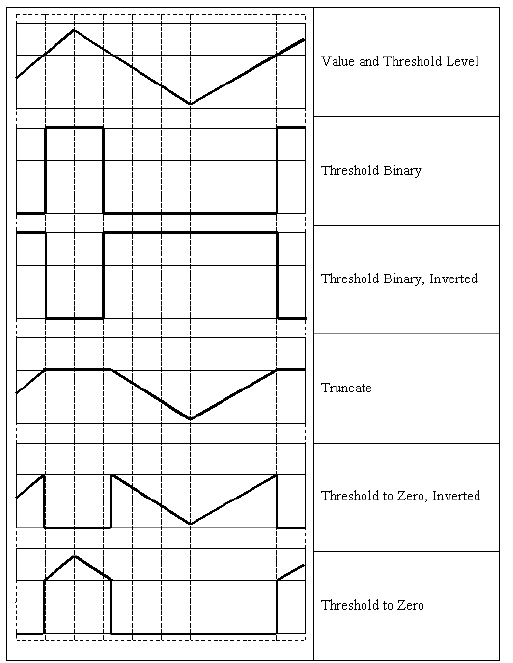
\includegraphics[width=0.5\textwidth]{pics/threshold.png}

See also: \cross{adaptiveThreshold}, \cross{findContours}, \cross{compare}, \cross{min}, \cross{max}

\cvfunc{watershed}\label{watershed}
Does marker-based image segmentation using watershed algrorithm

\begin{lstlisting}
void watershed( const Mat& image, Mat& markers );
\end{lstlisting}
\begin{description}
\cvarg{image}{The input 8-bit 3-channel image.} 
\cvarg{markers}{The input/output 32-bit single-channel image (map) of markers. It should have the same size as \texttt{image}}
\end{description}

The function implements one of the variants
of watershed, non-parametric marker-based segmentation algorithm,
described in \cite{Meyer92}. Before passing the image to the
function, user has to outline roughly the desired regions in the image
\texttt{markers} with positive ($>0$) indices, i.e. every region is
represented as one or more connected components with the pixel values
1, 2, 3 etc (such markers can be retrieved from a binary mask
using \cross{findContours}and \cross{drawContours}, see \texttt{watershed.cpp} demo).
The markers will be "seeds" of the future image
regions. All the other pixels in \texttt{markers}, which relation to the
outlined regions is not known and should be defined by the algorithm,
should be set to 0's. On the output of the function, each pixel in
markers is set to one of values of the "seed" components, or to -1 at
boundaries between the regions.

Note, that it is not necessary that every two neighbor connected
components are separated by a watershed boundary (-1's pixels), for
example, in case when such tangent components exist in the initial
marker image. Visual demonstration and usage example of the function
can be found in OpenCV samples directory; see \texttt{watershed.cpp} demo.

See also: \cross{findContours}


\subsection{Histograms}

\cvfunc{calcHist}\label{calcHist}
Calculates histogram of a set of arrays

\begin{lstlisting}
void calcHist( const Mat* arrays, int narrays,
               const int* channels, const Mat& mask,
               MatND& hist, int dims, const int* histSize,
               const float** ranges, bool uniform=true,
               bool accumulate=false );

void calcHist( const Mat* arrays, int narrays,
               const int* channels, const Mat& mask,
               SparseMat& hist, int dims, const int* histSize,
               const float** ranges, bool uniform=true,
               bool accumulate=false );
\end{lstlisting}
\begin{description}
\cvarg{arrays}{Source arrays. They all should have the same depth, \texttt{CV\_8U} or \texttt{CV\_32F}, and the same size. Each of them can have an arbitrary number of channels}
\cvarg{narrays}{The number of source arrays}
\cvarg{channels}{The list of \texttt{dims} channels that are used to compute the histogram. The first array channels are numerated from 0 to \texttt{arrays[0].channels()-1}, the second array channels are counted from \texttt{arrays[0].channels()} to \texttt{arrays[0].channels() + arrays[1].channels()-1} etc.}
\cvarg{mask}{The optional mask. If the matrix is not empty, it must be 8-bit array of the same size as \texttt{arrays[i]}. The non-zero mask elements mark the array elements that are counted in the histogram}
\cvarg{hist}{The output histogram, a dense or sparse \texttt{dims}-dimensional array}
\cvarg{dims}{The histogram dimensionality; must be positive and not greater than \texttt{CV\_MAX\_DIMS}(=32 in the current OpenCV version)}
\cvarg{histSize}{The array of histogram sizes in each dimension}
\cvarg{ranges}{The array of \texttt{dims} arrays of the histogram bin boundaries in each dimension. When the histogram is uniform (\texttt{uniform}=true), then for each dimension \texttt{i} it's enough to specify the lower (inclusive) boundary $L_0$ of the 0-th histogram bin and the upper (exclusive) boundary $U_{\texttt{histSize}[i]-1}$ for the last histogram bin \texttt{histSize[i]-1}. That is, in the case of uniform histogram each of \texttt{ranges[i]} is an array of 2 elements. When the histogram is not uniform (\texttt{uniform=false}), then each of \texttt{ranges[i]} contains \texttt{histSize[i]+1} elements: $L_0, U_0=L_1, U_1=L_2, ..., U_{\texttt{histSize[i]}-2}=L_{\texttt{histSize[i]}-1}, U_{\texttt{histSize[i]}-1}$. The array elements, which are not between $L_0$ and $U_{\texttt{histSize[i]}-1}$, are not counted in the histogram}
\cvarg{uniform}{Indicates whether the histogram is uniform or not, see above}
\cvarg{accumulate}{Accumulation flag. If it is set, the histogram is not cleared in the beginning (when it is allocated). This feature allows user to compute a single histogram from several sets of arrays, or to update the histogram in time}
\end{description}

The functions \texttt{calcHist} calculate the histogram of one or more
arrays. The elements of a tuple that is used to increment
a histogram bin are taken at the same location from the corresponding
input arrays. The sample below shows how to compute 2D Hue-Saturation histogram for a color imag

\begin{lstlisting}
#include <cv.h>
#include <highgui.h>

using namespace cv;

int main( int argc, char** argv )
{
    Mat src;
    if( argc != 2 || !(src=imread(argv[1], 1)).data )
        return -1;

    Mat hsv;
    cvtColor(src, hsv, CV_BGR2HSV);

    // let's quantize the hue to 30 levels
    // and the saturation to 32 levels
    int hbins = 30, sbins = 32;
    int histSize[] = {hbins, sbins};
    // hue varies from 0 to 179, see cvtColor
    float hranges[] = { 0, 180 };
    // saturation varies from 0 (black-gray-white) to
    // 255 (pure spectrum color)
    float sranges[] = { 0, 256 };
    float* ranges[] = { hranges, sranges };
    MatND hist;
    // we compute the histogram from the 0-th and 1-st channels
    int channels[] = {0, 1};
    
    calcHist( &hsv, 1, channels, Mat(), // do not use mask
        hist, 2, histSize, ranges,
        true, // the histogram is uniform
        false );
    double maxVal=0;
    minMaxLoc(hist, 0, &maxVal, 0, 0);
    
    int scale = 10;
    Mat histImg = Mat::zeros(sbins*scale, hbins*10, CV_8UC3);        

    for( int h = 0; h < hbins; h++ )
        for( int s = 0; s < sbins; s++ )
        {
            float binVal = hist.at<float>(h, s);
            int intensity = cvRound(binVal*255/maxValue);
            cvRectangle( histImg, Point(h*scale, s*scale),
                         Point( (h+1)*scale - 1, (s+1)*scale - 1),
                         Scalar::all(intensity),
                         CV_FILLED );
        }

    namedWindow( "Source", 1 );
    imshow( "Source", src );

    namedWindow( "H-S Histogram", 1 );
    imshow( "H-S Histogram", histImg );

    waitKey();
}
\end{lstlisting}


\cvfunc{calcBackProject}\label{calcBackProject}
Calculates the back projection of a histogram.

\begin{lstlisting}
void calcBackProject( const Mat* arrays, int narrays,
                      const int* channels, const MatND& hist,
                      Mat& backProject, const float** ranges,
                      double scale=1, bool uniform=true );
    
void calcBackProject( const Mat* arrays, int narrays,
                      const int* channels, const SparseMat& hist,
                      Mat& backProject, const float** ranges,
                      double scale=1, bool uniform=true );
\end{lstlisting}
\begin{description}
\cvarg{arrays}{Source arrays. They all should have the same depth, \texttt{CV\_8U} or \texttt{CV\_32F}, and the same size. Each of them can have an arbitrary number of channels}
\cvarg{narrays}{The number of source arrays}
\cvarg{channels}{The list of channels that are used to compute the back projection. The number of channels must match the histogram dimensionality. The first array channels are numerated from 0 to \texttt{arrays[0].channels()-1}, the second array channels are counted from \texttt{arrays[0].channels()} to \texttt{arrays[0].channels() + arrays[1].channels()-1} etc.}
\cvarg{hist}{The input histogram, a dense or sparse}
\cvarg{backProject}{Destination back projection aray; will be a single-channel array of the same size and the same depth as \texttt{arrays[0]}}
\cvarg{ranges}{The array of arrays of the histogram bin boundaries in each dimension. See \cross{calcHist}}
\cvarg{scale}{The optional scale factor for the output back projection}
\cvarg{uniform}{Indicates whether the histogram is uniform or not, see above}
\end{description}

The functions \texttt{calcBackProject} calculate the back project of the histogram. That is, similarly to \texttt{calcHist}, at each location \texttt{(x, y)} the function collects the values from the selected channels in the input images and finds the corresponding histogram bin. But instead of incrementing it, the function reads the bin value, scales it by \texttt{scale} and stores in \texttt{backProject(x,y)}. In terms of statistics, the function computes probability of each element value in respect with the empirical probability distribution represented by the histogram. Here is how, for example, you can find and track a bright-colored object in a scene:

\begin{enumerate}
 \item Before the tracking, show the object to the camera such that covers almost the whole frame. Calculate a hue histogram. The histogram will likely have a strong maximums, corresponding to the dominant colors in the object.
 \item During the tracking, calculate back projection of a hue plane of each input video frame using that pre-computed histogram. Threshold the back projection to suppress weak colors. It may also have sense to suppress pixels with non sufficient color saturation and too dark or too bright pixels.
 \item Find connected components in the resulting picture and choose, for example, the largest component.
\end{enumerate}

That is the approximate algorithm of \cross{CAMShift} color object tracker.

See also: \cross{calcHist}

\cross{compareHist}
Compares two histograms

\begin{lstlisting}
double compareHist( const MatND& H1, const MatND& H2, int method );
double compareHist( const SparseMat& H1, const SparseMat& H2, int method );
\end{lstlisting}
\begin{description}
\cvarg{H1}{The first compared histogram}
\cvarg{H2}{The second compared histogram of the same size as \texttt{H1}}
\cvarg{method}{The comparison method, one of the following:
\begin{description}
  \cvarg{CV\_COMP\_CORREL}{Correlation}
  \cvarg{CV\_COMP\_CHISQR}{Chi-Square}
  \cvarg{CV\_COMP\_INTERSECT}{Intersection}
  \cvarg{CV\_COMP\_BHATTACHARYYA}{Bhattacharyya distance}
\end{description}}
\end{description}

The functions \texttt{compareHist} compare two dense or two sparse histograms using the specified method:

\begin{description}
\item[Correlation (method=CV\_COMP\_CORREL)]
\[
d(H_1,H_2) = \frac
{\sum_I (H_1(I) - \bar{H_1}) (H_2(I) - \bar{H_2})}
{\sqrt{\sum_I(H_1(I) - \bar{H_1})^2 \sum_I(H_2(I) - \bar{H_2})^2}}
\]
where
\[
\bar{H_k} = \frac{1}{N} \sum_J H_k(J)
\]
and $N$ is the total number of histogram bins.

\item[Chi-Square (method=CV\_COMP\_CHISQR)]
\[ d(H_1,H_2) = \sum_I \frac{H_1(I)-H_2(I)}{H_1(I)+H_2(I)} \]

\item[Intersection (method=CV\_COMP\_INTERSECT)]
\[ d(H_1,H_2) = \sum_I \min (H_1(I), H_2(I)) \]

\item[Bhattacharyya distance (method=CV\_COMP\_BHATTACHARYYA)]
\[ d(H_1,H_2) = \sqrt{1 - \frac{1}{\bar{H_1} \bar{H_2} N^2} \sum_I \sqrt{H_1(I) \cdot H_2(I)}} \]

\end{description}

The function returns $d(H_1, H_2)$.

While the function works well with 1-, 2-, 3-dimensional dense histograms, it may not be suitable for high-dimensional sparse histograms, where, because of aliasing and sampling problems the coordinates of non-zero histogram bins can slightly shift. To compare such histograms or more general sparse configurations of weighted points, consider using the \cross{calcEMD} function.

\cvfunc{equalizeHist}\label{equalizeHist}
Equalizes the histogram of a grayscale image.

\begin{lstlisting}
void equalizeHist( const Mat& src, Mat& dst );
\end{lstlisting}
\begin{description}
\cvarg{src}{The source 8-bit single channel image}
\cvarg{dst}{The destination image; will have the same size and the same type as \texttt{src}}
\end{description}

The function \texttt{equalizeHist} equalizes the histogram of the input image using the following algorithm:

\begin{enumerate}
\item calculate the histogram $H$ for \texttt{src}.
\item normalize the histogram so that the sum of histogram bins is 255.
\item compute the integral of the histogram:
\[
H'_i = \sum_{0 \le j \le i} H(j)
\]
\item transform the image using $H'$ as a look-up table: $\texttt{dst}(x,y) = H'(\texttt{src}(x,y))$
\end{enumerate}

The algorithm normalizes the brightness and increases the contrast of the image.


\subsection{Feature Detection}

\cvfunc{cornerEigenValsAndVecs}\label{cornerEigenValsAndVecs}
Calculates eigenvalues and eigenvectors of image blocks for corner detection.

\begin{lstlisting}
void cornerEigenValsAndVecs( const Mat& src, Mat& dst,
                            int blockSize, int apertureSize,
                            int borderType=BORDER_DEFAULT );
\end{lstlisting}
\begin{description}
\cvarg{src}{Input single-channel 8-bit or floating-point image}
\cvarg{dst}{Image to store the results. It will have the same size as \texttt{src} and the type \texttt{CV\_32FC(6)}}
\cvarg{blockSize}{Neighborhood size (see discussion)}
\cvarg{apertureSize}{Aperture parameter for the \cross{Sobel} operator}
\cvarg{boderType}{Pixel extrapolation method; see \cross{borderInterpolate}}
\end{description}

For every pixel $p$, the function \texttt{cornerEigenValsAndVecs} considers a \texttt{blockSize} $\times$ \texttt{blockSize} neigborhood $S(p)$. It calculates the covariation matrix of derivatives over the neighborhood as:

\[
M = \begin{bmatrix}
\sum_{S(p)}(dI/dx)^2 & \sum_{S(p)}(dI/dx dI/dy)^2 \\
\sum_{S(p)}(dI/dx dI/dy)^2 & \sum_{S(p)}(dI/dy)^2
\end{bmatrix}
\]

Where the derivatives are computed using \cross{Sobel} operator.

After that it finds eigenvectors and eigenvalues of $M$ and stores them into destination image in the form
$(\lambda_1, \lambda_2, x_1, y_1, x_2, y_2)$ where
\begin{description}
\item[$\lambda_1, \lambda_2$]are the eigenvalues of $M$; not sorted
\item[$x_1, y_1$]are the eigenvectors corresponding to $\lambda_1$
\item[$x_2, y_2$]are the eigenvectors corresponding to $\lambda_2$
\end{description}

The output of the function can be used for robust edge or corner detection.

See also: \cross{cornerMinEigenVal}, \cross{cornerHarris}, \cross{preCornerDetect}

\cvfunc{cornerHarris}\label{cornerHarris}
Harris edge detector.

\begin{lstlisting}
void cornerHarris( const Mat& src, Mat& dst, int blockSize,
                  int apertureSize, double k,
                  int borderType=BORDER_DEFAULT );
\end{lstlisting}
\begin{description}
\cvarg{src}{Input single-channel 8-bit or floating-point image}
\cvarg{dst}{Image to store the Harris detector responses; will have type \texttt{CV\_32FC1} and the same size as \texttt{src}}
\cvarg{blockSize}{Neighborhood size (see the discussion of \cross{cornerEigenValsAndVecs})}
\cvarg{apertureSize}{Aperture parameter for the \cross{Sobel} operator}
\cvarg{k}{Harris detector free parameter. See the formula below}
\cvarg{boderType}{Pixel extrapolation method; see \cross{borderInterpolate}}
\end{description}

The function \texttt{cornerHarris} runs the Harris edge detector on the image. Similarly to \cross{cornerMinEigenVal} and \cross{cornerEigenValsAndVecs}, for each pixel $(x, y)$ it calculates a $2\times2$ gradient covariation matrix $M^{(x,y)}$ over a $\texttt{blockSize} \times \texttt{blockSize}$ neighborhood. Then, it computes the following characteristic:

\[
\texttt{dst}(x,y) = det(M^{(x,y)}) - k \, trace(M^{(x,y)})^2
\]

Corners in the image can be found as the local maxima of this response map.

\cvfunc{cornerMinEigenVal}\label{cornerMinEigenVal}
Calculates the minimal eigenvalue of gradient matrices for corner detection.

\begin{lstlisting}
void cornerMinEigenVal( const Mat& src, Mat& dst,
                        int blockSize, int apertureSize=3,
                        int borderType=BORDER_DEFAULT );
\end{lstlisting}
\begin{description}
\cvarg{src}{Input single-channel 8-bit or floating-point image}
\cvarg{dst}{Image to store the minimal eigenvalues; will have type \texttt{CV\_32FC1} and the same size as \texttt{src}}
\cvarg{blockSize}{Neighborhood size (see the discussion of \cross{cornerEigenValsAndVecs})}
\cvarg{apertureSize}{Aperture parameter for the \cross{Sobel} operator}
\cvarg{boderType}{Pixel extrapolation method; see \cross{borderInterpolate}}
\end{description}

The function \texttt{cornerMinEigenVal} is similar to \cross{cornerEigenValsAndVecs} but it calculates and stores only the minimal eigenvalue of the covariation matrix of derivatives, i.e. $min(\lambda_1, \lambda_2)$ in terms of the formulae in \cross{cornerEigenValsAndVecs} description.

\cvfunc{cornerSubPix}\label{cornerSubPix}
Refines the corner locations.

\begin{lstlisting}
void cornerSubPix( const Mat& image, vector<Point2f>& corners,
                   Size winSize, Size zeroZone,
                   TermCriteria criteria );
\end{lstlisting}
\begin{description}
\cvarg{image}{Input image}
\cvarg{corners}{Initial coordinates of the input corners; refined coordinates on output}
\cvarg{winSize}{Half of the side length of the search window. For example, if \texttt{winSize=Size(5,5)}, then a 5*2+1 $\times$ 5*2+1 = 11 $\times$ 11 search window would be used}
\cvarg{zeroZone}{Half of the size of the dead region in the middle of the search zone over which the summation in the formula below is not done. It is used sometimes to avoid possible singularities of the autocorrelation matrix. The value of (-1,-1) indicates that there is no such size}
\cvarg{criteria}{Criteria for termination of the iterative process of corner refinement. That is, the process of corner position refinement stops either after a certain number of iterations or when a required accuracy is achieved. The \texttt{criteria} may specify either of or both the maximum number of iteration and the required accuracy}
\end{description}

The function \texttt{cornerSubPix} iterates to find the sub-pixel accurate location of corners, or radial saddle points, as shown in on the picture below.

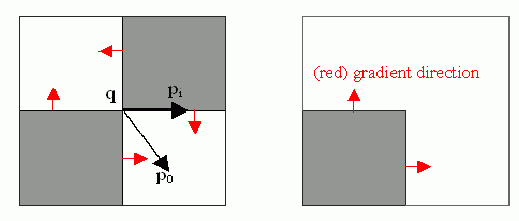
\includegraphics[width=1.0\textwidth]{pics/cornersubpix.png}

Sub-pixel accurate corner locator is based on the observation that every vector from the center $q$ to a point $p$ located within a neighborhood of $q$ is orthogonal to the image gradient at $p$ subject to image and measurement noise. Consider the expression:

\[
\epsilon_i = {DI_{p_i}}^T \cdot (q - p_i)
\]

where ${DI_{p_i}}$ is the image gradient at the one of the points $p_i$ in a neighborhood of $q$. The value of $q$ is to be found such that $\epsilon_i$ is minimized. A system of equations may be set up with $\epsilon_i$ set to zero:

\[
\sum_i(DI_{p_i} \cdot {DI_{p_i}}^T) - \sum_i(DI_{p_i} \cdot {DI_{p_i}}^T \cdot p_i)
\]

where the gradients are summed within a neighborhood ("search window") of $q$. Calling the first gradient term $G$ and the second gradient term $b$ gives:

\[
q = G^{-1} \cdot b
\]

The algorithm sets the center of the neighborhood window at this new center $q$ and then iterates until the center keeps within a set threshold.


\cvfunc{goodFeaturesToTrack}\label{goodFeaturesToTrack}
Determines strong corners on an image.

\begin{lstlisting}
void goodFeaturesToTrack( const Mat& image, vector<Point2f>& corners,
                         int maxCorners, double qualityLevel, double minDistance,
                         const Mat& mask=Mat(), int blockSize=3,
                         bool useHarrisDetector=false, double k=0.04 );
\end{lstlisting}
\begin{description}
\cvarg{image}{The input 8-bit or floating-point 32-bit, single-channel image}
\cvarg{corners}{The output vector of detected corners}
\cvarg{maxCorners}{The maximum number of corners to return. If there are more corners than that will be found, the strongest of them will be returned}
\cvarg{qualityLevel}{Characterizes the minimal accepted quality of image corners; the value of the parameter is multiplied by the by the best corner quality measure (which is the min eigenvalue, see \cross{cornerMinEigenVal}, or the Harris function response, see \cross{cornerHarris}). The corners, which quality measure is less than the product, will be rejected. For example, if the best corner has the quality measure = 1500, and the \texttt{qualityLevel=0.01}, then all the corners which quality measure is less than 15 will be rejected.}
\cvarg{minDistance}{The minimum possible Euclidean distance between the returned corners}
\cvarg{mask}{The optional region of interest. If the image is not empty (then it needs to have the type \texttt{CV\_8UC1} and the same size as \texttt{image}), it will specify the region in which the corners are detected}
\cvarg{blockSize}{Size of the averaging block for computing derivative covariation matrix over each pixel neighborhood, see \cross{cornerEigenValsAndVecs}}
\cvarg{useHarrisDetector}{Indicates, whether to use \href{cornerHarris}{Harris} operator or \cross{cornerMinEigenVal}}
\cvarg{k}{Free parameter of Harris detector}
\end{description}

The function finds the most prominent corners in the image or in the specified image region, as described
in \cite{Shi94}:
\begin{enumerate}
\item the function first calculates the corner quality measure at every source image pixel using the \cross{cornerMinEigenVal} or \cross{cornerHarris}
\item then it performs non-maxima suppression (the local maxima in $3\times 3$ neighborhood
are retained).
\item the next step rejects the corners with the minimal eigenvalue less than $\texttt{qualityLevel} \cdot \max_{x,y} qualityMeasureMap(x,y)$.
\item the remaining corners are then sorted by the quality measure in the descending order.
\item finally, the function throws away each corner $pt_j$ if there is a stronger corner $pt_i$ ($i < j$) such that the distance between them is less than \texttt{minDistance}
\end{enumerate}

The function can be used to initialize a point-based tracker of an object.

See also: \cross{cornerMinEigenVal}, \cross{cornerHarris}, \cross{calcOpticalFlowPyrLK}, \cross{estimateRigidMotion}, \cross{PlanarObjectDetector}, \cross{OneWayDescriptor}

\cvfunc{HoughCircles}\label{HoughCircles}
Finds circles in a grayscale image using a Hough transform.

\begin{lstlisting}
void HoughCircles( Mat& image, vector<Vec3f>& circles,
                 int method, double dp, double minDist,
                 double param1=100, double param2=100,
                 int minRadius=0, int maxRadius=0 );
\end{lstlisting}
\begin{description}
\cvarg{image}{The 8-bit, single-channel, grayscale input image}
\cvarg{circles}{The output vector of found circles. Each vector is encoded as 3-element floating-point vector $(x, y, radius)$}
\cvarg{method}{Currently, the only implemented method is \texttt{CV\_HOUGH\_GRADIENT}, which is basically \emph{21HT}, described in \cite{Yuen03}.}
\cvarg{dp}{The inverse ratio of the accumulator resolution to the image resolution. For example, if \texttt{dp=1}, the accumulator will have the same resolution as the input image, if \texttt{dp=2} - accumulator will have half as big width and height, etc}
\cvarg{minDist}{Minimum distance between the centers of the detected circles. If the parameter is too small, multiple neighbor circles may be falsely detected in addition to a true one. If it is too large, some circles may be missed}
\cvarg{param1}{The first method-specific parameter. in the case of \texttt{CV\_HOUGH\_GRADIENT} it is the higher threshold of the two passed to \cross{Canny} edge detector (the lower one will be twice smaller)}
\cvarg{param2}{The second method-specific parameter. in the case of \texttt{CV\_HOUGH\_GRADIENT} it is the accumulator threshold at the center detection stage. The smaller it is, the more false circles may be detected. Circles, corresponding to the larger accumulator values, will be returned first}
\cvarg{minRadius}{Minimum circle radius}
\cvarg{maxRadius}{Maximum circle radius}
\end{description}

The function \texttt{houghCircles} finds circles in a grayscale image using some modification of Hough transform. Here is a short usage example:

\begin{lstlisting}
#include <cv.h>
#include <highgui.h>
#include <math.h>

using namespace cv;

int main(int argc, char** argv)
{
    Mat img, gray;
    if( argc != 2 && !(img=imread(argv[1], 1)).data)
        return -1;
    cvtColor(img, gray, CV_BGR2GRAY);
    // smooth it, otherwise a lot of false circles may be detected
    GaussianBlur( gray, gray, 9, 9, 2, 2 );
    vector<Vec3f> circles;
    houghCircles(gray, circles, CV_HOUGH_GRADIENT,
                 2, gray->rows/4, 200, 100 );
    for( size_t i = 0; i < circles.size(); i++ )
    {
         Point center(cvRound(circles[i][0]), cvRound(circles[i][1]));
         int radius = cvRound(circles[i][2]);
         // draw the circle center
         circle( img, center, 3, Scalar(0,255,0), -1, 8, 0 );
         // draw the circle outline
         circle( img, center, radius, Scalar(0,0,255), 3, 8, 0 );
    }
    namedWindow( "circles", 1 );
    imshow( "circles", img );
    return 0;
}
\end{lstlisting}

Note that usually the function detects the circles' centers well, however it may fail to find the correct radii. You can assist the function by specifying the radius range (\texttt{minRadius} and \texttt{maxRadius}) if you know it, or you may ignore the returned radius, use only the center and find the correct radius using some additional procedure.

\see also: \cross{fitEllipse}, \cross{minEnclosingCircle}

\cvfunc{HoughLines}\label{HoughLines}
Finds lines in a binary image using standard Hough transform.

\begin{lstlisting}
void HoughLines( Mat& image, vector<Vec2f>& lines,
                 double rho, double theta, int threshold,
                 double srn=0, double stn=0 );
\end{lstlisting}
\begin{description}
\cvarg{image}{The 8-bit, single-channel, binary source image. The image may be modified by the function}
\cvarg{lines}{The output vector of lines. Each line is represented by a two-element vector $(\rho, \theta)$. $\rho$ is the distance from the coordinate origin $(0,0)$ (top-left corner of the image) and $\theta$ is the line rotation angle in radians (0 $\sim$ vertical line, $\pi/2 \sim$ horizontal line)}
\cvarg{rho}{Distance resolution of the accumulator in pixels}
\cvarg{theta}{Angle resolution of the accumulator in radians}
\cvarg{threshold}{The accumulator threshold parameter. Only those lines are returned that get enough votes (>\texttt{threshold})}
\cvarg{srn}{For the multi-scale Hough transform it is the divisor for the distance resolution \texttt{rho}. The coarse accumulator distance resolution will be \texttt{rho} and the accurate accumulator resolution will be \texttt{rho/srn}. If both \texttt{srn=0} and \texttt{stn=0} then the classical Hough transform is used, otherwise both these parameters should be positive.}
\cvarg{stn}{For the multi-scale Hough transform it is the divisor for the distance resolution \texttt{theta}}
\end{description}

The function \texttt{HoughLines} implements standard or standard multi-scale Hough transform algorithm for line detection. See \cross{HoughLinesP} for the code example.


\cvfunc{HoughLinesP}\label{HoughLinesP}
Finds lines segments in a binary image using probabilistic Hough transform.

\begin{lstlisting}
void HoughLinesP( Mat& image, vector<Vec4i>& lines,
                  double rho, double theta, int threshold,
                  double minLineLength=0, double maxLineGap=0 );
\end{lstlisting}
\begin{description}
\cvarg{image}{The 8-bit, single-channel, binary source image. The image may be modified by the function}
\cvarg{lines}{The output vector of lines. Each line is represented by a 4-element vector $(x_1, y_1, x_2, y_2)$, where $(x_1,y_1)$ and $(x_2, y_2)$ are the ending points of each line segment detected.}
\cvarg{rho}{Distance resolution of the accumulator in pixels}
\cvarg{theta}{Angle resolution of the accumulator in radians}
\cvarg{threshold}{The accumulator threshold parameter. Only those lines are returned that get enough votes (>\texttt{threshold})}
\cvarg{minLineLength}{The minimum line length. Line segments shorter than that will be rejected}
\cvarg{maxLineGap}{The maximum allowed gap between points on the same line to link them.}
\end{description}

The function \texttt{HoughLinesP} implements probabilistic Hough transform algorithm for line detection, described in \cite[Matas98]. Below is line detection example:

\begin{lstlisting}
/* This is a standalone program. Pass an image name as a first parameter
of the program.  Switch between standard and probabilistic Hough transform
by changing "#if 1" to "#if 0" and back */
#include <cv.h>
#include <highgui.h>
#include <math.h>

using namespace cv;

int main(int argc, char** argv)
{
    Mat src, dst, color_dst;
    if( argc != 2 || !(src=imread(argv[1], 0)).data)
        return -1;
        
    Canny( src, dst, 50, 200, 3 );
    cvtColor( dst, color_dst, CV_GRAY2BGR );    
        
#if 0
    vector<Vec2f> lines;
    HoughLines( dst, lines, 1, CV_PI/180, 100 );

    for( size_t i = 0; i < lines.size(); i++ )
    {
        float rho = lines[i][0];
        float theta = lines[i][1];
        double a = cos(theta), b = sin(theta);
        double x0 = a*rho, y0 = b*rho;
        Point pt1(cvRound(x0 + 1000*(-b)),
                  cvRound(y0 + 1000*(a)));
        Point pt2(cvRound(x0 - 1000*(-b)),
                  cvRound(y0 - 1000*(a)));
        line( color_dst, pt1, pt2, Scalar(0,0,255), 3, 8 );
    }
#else
    vector<Vec4i> lines;
    HoughLinesP( dst, lines, 1, CV_PI/180, 80, 30, 10 );
    for( size_t i = 0; i < lines.size(); i++ )
    {
        line( color_dst, Point(lines[i][0], lines[i][1]),
            Point(lines[i][2], lines[i][3]), Scalar(0,0,255), 3, 8 );
    }
#endif
    namedWindow( "Source", 1 );
    imshow( "Source", src );

    namedWindow( "Detected Lines", 1 );
    imshow( "Detected Lines", color_dst );

    waitKey(0);
    return 0;
}
\end{lstlisting}


This is the sample picture the function parameters have been tuned for:

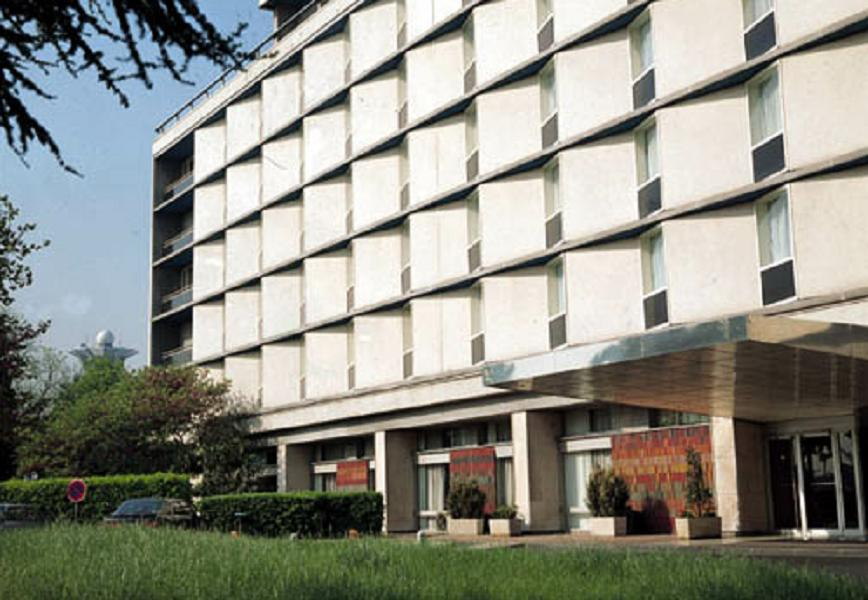
\includegraphics[width=0.5\textwidth]{pics/building.jpg}

And this is the output of the above program in the case of probabilistic Hough transform

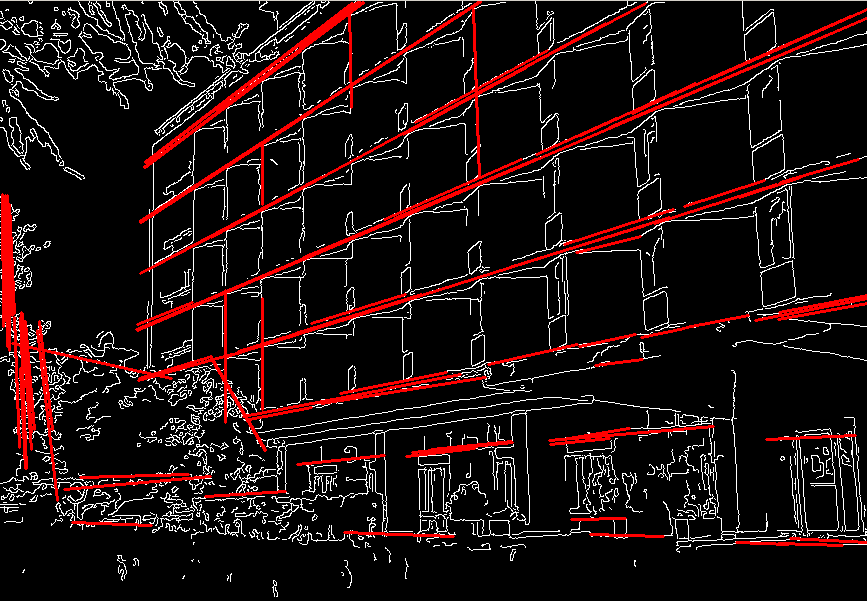
\includegraphics[width=0.5\textwidth]{pics/houghp.png}

\cvfunc{perCornerDetect}\label{perCornerDetect}
Calculates the feature map for corner detection

\begin{lstlisting}
void preCornerDetect( const Mat& src, Mat& dst, int apertureSize,
                     int borderType=BORDER_DEFAULT );
\end{lstlisting}
\begin{description}
\cvarg{src}{The source single-channel 8-bit of floating-point image}
\cvarg{dst}{The output image; will have type \texttt{CV\_32F} and the same size as \texttt{src}}
\cvarg{apertureSize}{Aperture size of \cross{Sobel}}
\cvarg{borderType}{The pixel extrapolation method; see \cross{borderInterpolate}}
\end{description}

The function \texttt{preCornerDetect} calculates the complex spatial derivative-based function of the source image

\[
\texttt{dst} = (D_x \texttt{src})^2 \cdot D_{yy} \texttt{src} + (D_y \texttt{src})^2 \cdot D_{xx} \texttt{src} - 2 D_x \texttt{src} \cdot D_y \texttt{src} \cdot D_{xy} \texttt{src}
\]

where $D_x$, $D_y$ are the first image derivatives, $D_xx$, $D_yy$ are the second image derivatives and $D_xy$ is the mixed derivative.

The corners can be found as local maximums of the functions, as shown below:

\begin{lstlisting}
Mat corners, dilated_corners;
preCornerDetect(image, corners, 3);
// dilation with 3x3 rectangular structuring element
dilate(corners, dilated_corners, Mat(), 1);
Mat corner_mask = corners == dilated_corners;
\end{lstlisting}


\cvfunc{KeyPoint}\label{KeyPoint}
Data structure for interest point detectors

\begin{lstlisting}
class KeyPoint
{
public:
    // default constructor
    KeyPoint();
    // two complete constructors
    KeyPoint(Point2f _pt, float _size, float _angle=-1,
            float _response=0, int _octave=0, int _class_id=-1);
    KeyPoint(float x, float y, float _size, float _angle=-1,
             float _response=0, int _octave=0, int _class_id=-1);
    // coordinate of the point
    Point2f pt;
    // feature size
    float size;
    // feature orintation in degrees
    // (has negative value if the orientation
    // is not defined/not computed)
    float angle;
    // feature strength
    // (can be used to select only
    // the most prominent key points)
    float response;
    // scale-space octave in which the feature has been found;
    // may correlate with the size
    int octave;
    // point class (can be used by feature
    // classifiers or object detectors)
    int class_id;
};

// reading/writing a vector of keypoints to a file storage
void write(FileStorage& fs, const string& name, const vector<KeyPoint>& keypoints);
void read(const FileNode& node, vector<KeyPoint>& keypoints);    
\end{lstlisting}


\cvfunc{MSER}\label{MSER}
Maximally-Stable Extremal Region Extractor

\begin{lstlisting}
class MSER : public CvMSERParams
{
public:
    // default constructor
    MSER();
    // constructor that initializes all the algorithm parameters
    MSER( int _delta, int _min_area, int _max_area,
          float _max_variation, float _min_diversity,
          int _max_evolution, double _area_threshold,
          double _min_margin, int _edge_blur_size );
    // runs the extractor on the specified image; returns the MSERs,
    // each encoded as a contour (vector<Point>, see findContours)
    // the optional mask marks the area where MSERs are searched for
    void operator()(Mat& image, vector<vector<Point> >& msers, const Mat& mask) const;
};
\end{lstlisting}

The class encapsulates all the parameters of MSER (see \url{http://en.wikipedia.org/wiki/Maximally_stable_extremal_regions}) extraction algorithm. 

\cvfunc{SURF}\label{SURF}
Class for extracting Speeded Up Robust Features from an image.

\begin{lstlisting}
class SURF : public CvSURFParams
{
public:
    // default constructor
    SURF();
    // constructor that initializes all the algorithm parameters
    SURF(double _hessianThreshold, int _nOctaves=4,
         int _nOctaveLayers=2, bool _extended=false);
    // returns the number of elements in each descriptor (64 or 128)
    int descriptorSize() const;
    // detects keypoints using fast multi-scale Hessian detector
    void operator()(const Mat& img, const Mat& mask,
                    vector<KeyPoint>& keypoints) const;
    // detects keypoints and computes the SURF descriptors for them
    void operator()(const Mat& img, const Mat& mask,
                    vector<KeyPoint>& keypoints,
                    vector<float>& descriptors,
                    bool useProvidedKeypoints=false) const;
};
\end{lstlisting}

The class \texttt{SURF} implements Speeded Up Robust Features descriptor described \cite{Bay06}.
There is fast multi-scale Hessian keypoint detector that can be used to find the keypoints
(which is the default option), but the descriptors can be also computed for the user-specified keypoints.
The function can be used for object tracking and localization, image stitching etc. See the
\texttt{find\_obj.cpp} demo in OpenCV samples directory.


\cvfunc{StarDetector}\label{StarDetector}
Implements Star keypoint detector

\begin{lstlisting}
class StarDetector : CvStarDetectorParams
{
public:
    // default constructor
    StarDetector();
    // the full constructor initialized all the algorithm parameters:
    // maxSize - maximum size of the features. The following 
    //      values of the parameter are supported:
    //      4, 6, 8, 11, 12, 16, 22, 23, 32, 45, 46, 64, 90, 128
    // responseThreshold - threshold for the approximated laplacian,
    //      used to eliminate weak features. The larger it is,
    //      the less features will be retrieved
    // lineThresholdProjected - another threshold for the laplacian to 
    //      eliminate edges
    // lineThresholdBinarized - another threshold for the feature 
    //      size to eliminate edges.
    // The larger the 2 threshold, the more points you get.
    StarDetector(int maxSize, int responseThreshold,
                 int lineThresholdProjected,
                 int lineThresholdBinarized,
                 int suppressNonmaxSize);

    // finds keypoints in an image
    void operator()(const Mat& image, vector<KeyPoint>& keypoints) const;
};
\end{lstlisting}

The class implements a modified version of CenSurE keypoint detector described in
\cite{Agrawal08}

\subsection{Motion Analysis}

\cvfunc{accumulate}\label{accumulate}
Adds image to the accumulator.

\begin{lstlisting}
void accumulate( const Mat& src, Mat& dst, const Mat& mask=Mat() );
\end{lstlisting}
\begin{description}
\cvarg{src}{The input image, 1- or 3-channel, 8-bit or 32-bit floating point}
\cvarg{dst}{The accumulator image with the same number of channels as input image, 32-bit or 64-bit floating-point}
\cvarg{mask}{Optional operation mask}
\end{description}

The function adds \texttt{src}, or some of its elements, to \texttt{dst}:

\[ \texttt{dst}(x,y) \leftarrow \texttt{dst}(x,y) + \texttt{src}(x,y) \quad \text{if} \quad \texttt{mask}(x,y) \ne 0 \]

The function supports multi-channel images; each channel is processed independently.

The functions \texttt{accumulate*} can be used, for example, to collect statistic of background of a scene, viewed by a still camera, for the further foreground-background segmentation.

See also: \cross{accumulateSquare}, \cross{accumulateProduct}, \cross{accumulateWeighted}

\cvfunc{accumulateSquare}\label{accumulateSquare}
Adds the square of the source image to the accumulator.

\begin{lstlisting}
void accumulateSquare( const Mat& src, Mat& dst, const Mat& mask=Mat() );
\end{lstlisting}
\begin{description}
\cvarg{src}{The input image, 1- or 3-channel, 8-bit or 32-bit floating point}
\cvarg{dst}{The accumulator image with the same number of channels as input image, 32-bit or 64-bit floating-point}
\cvarg{mask}{Optional operation mask}
\end{description}

The function \texttt{accumulateSquare} adds the input image \texttt{src} or its selected region, raised to power 2, to the accumulator \texttt{dst}:

\[ \texttt{dst}(x,y) \leftarrow \texttt{dst}(x,y) + \texttt{src}(x,y)^2 \quad \text{if} \quad \texttt{mask}(x,y) \ne 0 \]

The function supports multi-channel images; each channel is processed independently.

See also: \cross{accumulateSquare}, \cross{accumulateProduct}, \cross{accumulateWeighted}

\cvfunc{accumulateProduct}\label{accumulateProduct}
Adds the per-element product of two input images to the accumulator.

\begin{lstlisting}
void accumulateProduct( const Mat& src1, const Mat& src2,
                        Mat& dst, const Mat& mask=Mat() );
\end{lstlisting}
\begin{description}
\cvarg{src1}{The first input image, 1- or 3-channel, 8-bit or 32-bit floating point}
\cvarg{src2}{The second input image of the same type and the same size as \texttt{src1}}
\cvarg{dst}{Accumulator with the same number of channels as input images, 32-bit or 64-bit floating-point}
\cvarg{mask}{Optional operation mask}
\end{description}

The function \texttt{accumulateProduct} adds the product of 2 images or their selected regions to the accumulator \texttt{dst}:

\[ \texttt{dst}(x,y) \leftarrow \texttt{dst}(x,y) + \texttt{src1}(x,y) \cdot \texttt{src2}(x,y) \quad \text{if} \quad \texttt{mask}(x,y) \ne 0 \]

The function supports multi-channel images; each channel is processed independently.

See also: \cross{accumulate}, \cross{accumulateSquare}, \cross{accumulateWeighted}

\cvfunc{accumulateWeighted}\label{accumulateWeighted}
Updates the running average.

\begin{lstlisting}
void accumulateWeighted( const Mat& src, Mat& dst,
                         double alpha, const Mat& mask=Mat() );
\end{lstlisting}
\begin{description}
\cvarg{src}{The input image, 1- or 3-channel, 8-bit or 32-bit floating point}
\cvarg{dst}{The accumulator image with the same number of channels as input image, 32-bit or 64-bit floating-point}
\cvarg{alpha}{Weight of the input image}
\cvarg{mask}{Optional operation mask}
\end{description}

The function \texttt{accumulateWeightedg} calculates the weighted sum of the input image
\texttt{src} and the accumulator \texttt{dst} so that \texttt{dst}
becomes a running average of frame sequence:

\[ \texttt{dst}(x,y) \leftarrow (1-\texttt{alpha}) \cdot \texttt{dst}(x,y) + \texttt{alpha} \cdot \texttt{src}(x,y) \quad \text{if} \quad \texttt{mask}(x,y) \ne 0 \]

that is, \texttt{alpha} regulates the update speed (how fast the accumulator "forgets" about earlier images).
The function supports multi-channel images; each channel is processed independently.

See also: \cross{accumulate}, \cross{accumulateSquare}, \cross{accumulateProduct}

\cvfunc{calcOpticalFlowPyrLK}\label{calcOpticalFlowPyrLK}
Calculates the optical flow for a sparse feature set using the iterative Lucas-Kanade method with pyramids

\begin{lstlisting}
void calcOpticalFlowPyrLK( const Mat& prevImg, const Mat& nextImg,
        const vector<Point2f>& prevPts, vector<Point2f>& nextPts,
        vector<uchar>& status, vector<float>& err, Size winSize=Size(15,15),
        int maxLevel=3, TermCriteria criteria=TermCriteria(
            TermCriteria::COUNT+TermCriteria::EPS, 30, 0.01),
        double derivLambda=0.5, int flags=0 );
enum { OPTFLOW_USE_INITIAL_FLOW=4 };
\end{lstlisting}
\begin{description}
\cvarg{prevImg}{The first 8-bit single-channel or 3-channel input image}
\cvarg{nextImg}{The second input image of the same size and the same type as \texttt{prevImg}}
\cvarg{prevPts}{Vector of points for which the flow needs to be found}
\cvarg{nextPts}{The output vector of points containing the calculated new positions of the input features in the second image}
\cvarg{status}{The output status vector. Each element of the vector is set to 1 if the flow for the corresponding features has been found, 0 otherwise}
\cvarg{err}{The output vector that will contain the difference between patches around the original and moved points}
\cvarg{winSize}{Size of the search window at each pyramid level}
\cvarg{maxLevel}{0-based maximal pyramid level number. If 0, pyramids are not used (single level), if 1, two levels are used etc.}
\cvarg{criteria}{Specifies the termination criteria of the iterative search algorithm (after the specified maximum number of iterations \texttt{criteria.maxCount} or when the search window moves by less than \texttt{criteria.epsilon}}
\cvarg{derivLambda}{The relative weight of the spatial image derivatives impact to the optical flow estimation. If \texttt{derivLambda=0}, only the image intensity is used, if \texttt{derivLambda=1}, only derivatives are used. Any other values between 0 and 1 means that both derivatives and the image intensity are used (in the corresponding proportions).}
\cvarg{flags}{The operation flags:
\begin{description}
  \cvarg{OPTFLOW\_USE\_INITIAL\_FLOW}{use initial estimations stored in \texttt{nextPts}. If the flag is not set, then initially $\texttt{nextPts}\leftarrow\texttt{prevPts}$}
\end{description}}
\end{description}

The function \texttt{calcOpticalFlowPyrLK} implements the sparse iterative version of the Lucas-Kanade optical flow in pyramids, see \cite{Bouguet00}.

\cvfunc{calcOpticalFlowFarneback}\label{calcOpticalFlowFarneback}
Computes dense optical flow using Gunnar Farneback's algorithm

\begin{lstlisting}
void calcOpticalFlowFarneback( const Mat& prevImg, const Mat& nextImg,
                               Mat& flow, double pyrScale, int levels, int winsize,
                               int iterations, int poly_n, double poly_sigma, int flags );
enum { OPTFLOW_FARNEBACK_GAUSSIAN=256 };
\end{lstlisting}
\begin{description}
\cvarg{prevImg}{The first 8-bit single-channel input image}
\cvarg{nextImg}{The second input image of the same size and the same type as \texttt{prevImg}}
\cvarg{flow}{The computed flow image; will have the same size as \texttt{prevImg} and type \texttt{CV\_32FC2}}
\cvarg{pyrScale}{Specifies the image scale (<1) to build the pyramids for each image. \texttt{pyrScale=0.5} means the classical pyramid, where each next layer is twice smaller than the previous}
\cvarg{levels}{The number of pyramid layers, including the initial image. \texttt{levels=1} means that no extra layers are created and only the original images are used}
\cvarg{winsize}{The averaging window size; The larger values increase the algorithm robustness to image noise and give more chances for fast motion detection, but yield more blurred motion field}
\cvarg{iterations}{The number of iterations the algorithm does at each pyramid level}
\cvarg{poly\_n}{Size of the pixel neighborhood used to find polynomial expansion in each pixel. The larger values mean that the image will be approximated with smoother surfaces, yielding more robust algorithm and more blurred  motion field. Typically, \texttt{poly\_n}=5 or 7}
\cvarg{poly\_sigma}{Standard deviation of the Gaussian that is used to smooth derivatives that are used as a basis for the polynomial expansion. For \texttt{poly\_n=5} you can set \texttt{poly\_sigma=1.1}, for \texttt{poly\_n=7} a good value would be \texttt{poly\_sigma=1.5}}
\cvarg{flags}{The operation flags; can be a combination of the following:
\begin{description}
    \cvarg{OPTFLOW\_USE\_INITIAL\_FLOW}{Use the input \texttt{flow} as the initial flow approximation}
    \cvarg{OPTFLOW\_FARNEBACK\_GAUSSIAN}{Use a Gaussian $\texttt{winsize} \times \texttt{winsize}$filter instead of box filter of the same size for optical flow estimation. Usually, this option gives more accurate flow than with a box filter, at the cost of lower speed (and normally \texttt{winsize} for a Gaussian window should be set to a larger value to achieve the same level of robustness)}
\end{description}}
\end{description}

The function finds optical flow for each \texttt{prevImg} pixel using the alorithm so that

\[\texttt{prevImg}(x,y) \sim \texttt{nextImg}(\texttt{flow}(x,y)[0], \texttt{flow}(x,y)[1])\]


\cvfunc{updateMotionHistory}\label{updateMotionHistory}
Updates the motion history image by a moving silhouette.

\begin{lstlisting}
void updateMotionHistory( const Mat& silhouette, Mat& mhi,
                          double timestamp, double duration );
\end{lstlisting}
\begin{description}
\cvarg{silhouette}{Silhouette mask that has non-zero pixels where the motion occurs}
\cvarg{mhi}{Motion history image, that is updated by the function (single-channel, 32-bit floating-point)}
\cvarg{timestamp}{Current time in milliseconds or other units}
\cvarg{duration}{Maximal duration of the motion track in the same units as \texttt{timestamp}}
\end{description}

The function \texttt{updateMotionHistory} updates the motion history image as following:

\[
\texttt{mhi}(x,y)=\forkthree
{\texttt{timestamp}}{if $\texttt{silhouette}(x,y) \ne 0$}
{0}{if $\texttt{silhouette}(x,y) = 0$ and $\texttt{mhi} < (\texttt{timestamp} - \texttt{duration})$}
{\texttt{mhi}(x,y)}{otherwise}
\]
That is, MHI pixels where motion occurs are set to the current \texttt{timestamp}, while the pixels where motion happened last time a long time ago are cleared.

The function, together with \cross{calcMotionGradient} and \cross{calcGlobalOrientation}, implements the motion templates technique, described in \cite{Davis97} and \cite{Bradski00}.
See also the OpenCV sample \texttt{motempl.c} that demonstrates the use of all the motion template functions.

\cvfunc{calcMotionGradient}\label{calcMotionGradient}
Calculates the gradient orientation of a motion history image.

\begin{lstlisting}
void calcMotionGradient( const Mat& mhi, Mat& mask,
                         Mat& orientation,
                         double delta1, double delta2,
                         int apertureSize=3 );
\end{lstlisting}
\begin{description}
\cvarg{mhi}{Motion history single-channel floating-point image}
\cvarg{mask}{The output mask image; will have the type \texttt{CV\_8UC1} and the same size as \texttt{mhi}. Its non-zero elements will mark pixels where the motion gradient data is correct}
\cvarg{orientation}{The output motion gradient orientation image; will have the same type and the same size as \texttt{mhi}. Each pixel of it will the motion orientation in degrees, from 0 to 360.}
\cvarg{delta1, delta2}{The minimal and maximal allowed difference between \texttt{mhi} values within a pixel neighorhood. That is, the function finds the minimum ($m(x,y)$) and maximum ($M(x,y)$) \texttt{mhi} values over $3 \times 3$ neighborhood of each pixel and marks the motion orientation at $(x, y)$ as valid only if
\[
\min(\texttt{delta1} , \texttt{delta2} ) \le M(x,y)-m(x,y) \le \max(\texttt{delta1} ,\texttt{delta2}).
\]}
\cvarg{apertureSize}{The aperture size of \cross{Sobel} operator}
\end{description}

The function \texttt{calcMotionGradient} calculates the gradient orientation at each pixel $(x, y)$ as:

\[
\texttt{orientation}(x,y)=\arctan{\frac{d\texttt{mhi}/dy}{d\texttt{mhi}/dx}}
\]

(in fact, \cross{fastArctan} and \cross{phase} are used, so that the computed angle is measured in degrees and covers the full range 0..360). Also, the \texttt{mask} is filled to indicate pixels where the computed angle is valid.

\cvfunc{calcGlobalOrientation}\label{calcGlobalOrientation}
Calculates the global motion orientation in some selected region.

\begin{lstlisting}
double calcGlobalOrientation( const Mat& orientation, const Mat& mask,
                              const Mat& mhi, double timestamp,
                              double duration );
\end{lstlisting}
\begin{description}
\cvarg{orientation}{Motion gradient orientation image, calculated by the function \cross{calcMotionGradient}}
\cvarg{mask}{Mask image. It may be a conjunction of a valid gradient mask, also calculated by \cross{calcMotionGradient}, and the mask of the region, whose direction needs to be calculated}
\cvarg{mhi}{The motion history image, calculated by \cross{updateMotionHistory}}
\cvarg{timestamp}{The timestamp passed to \cross{updateMotionHistory}}
\cvarg{duration}{Maximal duration of motion track in milliseconds, passed to \cross{updateMotionHistory}}
\end{description}

The function \texttt{calcGlobalOrientation} calculates the average
motion direction in the selected region and returns the angle between
0 degrees  and 360 degrees. The average direction is computed from
the weighted orientation histogram, where a recent motion has larger
weight and the motion occurred in the past has smaller weight, as recorded in \texttt{mhi}.

\cvfunc{CamShift}\label{CamShift}
Finds the object center, size, and orientation

\begin{lstlisting}
RotatedRect CamShift( const Mat& probImage, Rect& window,
                      TermCriteria criteria );
\end{lstlisting}
\begin{description}
\cvarg{probImage}{Back projection of the object histogram; see \cross{calcBackProject}}
\cvarg{window}{Initial search window}
\cvarg{criteria}{Stop criteria for the underlying \cross{meanShift}}
\end{description}

The function \texttt{CamShift} implements the CAMSHIFT object tracking algrorithm
\cross{Bradski98}.
First, it finds an object center using \cross{meanShift} and then adjust the window size and finds the optimal rotation. The function returns the rotated rectangle structure that includes the object position, size and the orientation. The next position of the search window can be obtained with \texttt{RotatedRect::boundingRect()}.

See the OpenCV sample \texttt{camshiftdemo.c} that tracks colored objects.

\cvfunc{meanShift}\label{meanShift}
Finds the object on a back projection image.

\begin{lstlisting}
int meanShift( const Mat& probImage, Rect& window,
               TermCriteria criteria );
\end{lstlisting}
\begin{description}
\cvarg{probImage}{Back projection of the object histogram; see \cross{calcBackProject}}
\cvarg{window}{Initial search window}
\cvarg{criteria}{The stop criteria for the iterative search algorithm}
\end{description}

The function implements iterative object search algorithm. It takes the object back projection on input and the initial position. The mass center in \texttt{window} of the back projection image is computed and the search window center shifts to the mass center. The procedure is repeated until the specified number of iterations \texttt{criteria.maxCount} is done or until the window center shifts by less than \texttt{criteria.epsilon}. The algorithm is used inside \cross{CamShift} and, unlike \cross{CamShift}, the search window size or orientation do not change during the search. You can simply pass the output of \cross{calcBackProject} to this function, but better results can be obtained if you pre-filter the back projection and remove the noise (e.g. by retrieving connected components with \cross{findContours}, throwing away contours with small area (\cross{contourArea}) and rendering the  remaining contours with \cross{drawContours})


\cvfunc{KalmanFilter}\label{KalmanFilter}
Kalman filter class

\begin{lstlisting}
class KalmanFilter
{
public:
    KalmanFilter();
    KalmanFilter(int dynamParams, int measureParams, int controlParams=0);
    void init(int dynamParams, int measureParams, int controlParams=0);

    // predicts statePre from statePost
    const Mat& predict(const Mat& control=Mat());
    // corrects statePre based on the input measurement vector
    // and stores the result to statePost. 
    const Mat& correct(const Mat& measurement);

    Mat statePre;           // predicted state (x'(k)):
                            //    x(k)=A*x(k-1)+B*u(k)
    Mat statePost;          // corrected state (x(k)):
                            //    x(k)=x'(k)+K(k)*(z(k)-H*x'(k))
    Mat transitionMatrix;   // state transition matrix (A)
    Mat controlMatrix;      // control matrix (B)
                            //   (it is not used if there is no control)
    Mat measurementMatrix;  // measurement matrix (H)
    Mat processNoiseCov;    // process noise covariance matrix (Q)
    Mat measurementNoiseCov;// measurement noise covariance matrix (R)
    Mat errorCovPre;        // priori error estimate covariance matrix (P'(k)):
                            //    P'(k)=A*P(k-1)*At + Q)*/
    Mat gain;               // Kalman gain matrix (K(k)):
                            //    K(k)=P'(k)*Ht*inv(H*P'(k)*Ht+R)
    Mat errorCovPost;       // posteriori error estimate covariance matrix (P(k)):
                            //    P(k)=(I-K(k)*H)*P'(k)
    ...
};
\end{lstlisting}

The class implements standard Kalman filter \url{http://en.wikipedia.org/wiki/Kalman_filter}. However, you can modify \texttt{transitionMatrix}, \texttt{controlMatrix} and \texttt{measurementMatrix} to get the extended Kalman filter functionality. See the OpenCV sample \texttt{kalman.c}


\subsection{Structural Analysis and Shape Descriptors}

\cvfunc{moments}\label{moments}
Calculates all of the moments up to the third order of a polygon or rasterized shape.

\begin{lstlisting}
Moments moments( const Mat& array, bool binaryImage=false );

class Moments
{
public:
    Moments();
    Moments(double m00, double m10, double m01, double m20, double m11,
            double m02, double m30, double m21, double m12, double m03 );
    Moments( const CvMoments& moments );
    operator CvMoments() const;
    
    // spatial moments
    double  m00, m10, m01, m20, m11, m02, m30, m21, m12, m03;
    // central moments
    double  mu20, mu11, mu02, mu30, mu21, mu12, mu03;
    // central normalized moments
    double  nu20, nu11, nu02, nu30, nu21, nu12, nu03;
};
\end{lstlisting}
\begin{description}
\cvarg{array}{A raster image (single-channel, 8-bit or floating-point 2D array) or an array
    ($1 \times N$ or $N \times 1$) of 2D points (\href{Point\_}{Point} or \href{Point\_}{Point2f})}
\cvarg{binaryImage}{(For images only) If it is true, then all the non-zero image pixels are treated as 1's}
\end{description}

The function \texttt{moments} computes moments, up to the 3rd order, of a vector shape or a rasterized shape.
In case of a raster image, the spatial moments $\texttt{Moments::m}_ji$ are computed as:

\[\texttt{m}_{ji}=\sum_{x,y} (\texttt{array}(x,y) \cdot x^j \cdot y^i),\]

the central moments $\texttt{Moments::mu}_ji$ are computed as:
\[\texttt{mu}_{ji}=\sum_{x,y} (\texttt{array}(x,y) \cdot (x - \bar{x})^j \cdot (y - \bar{y})^i)\]
where $(\bar{x}, \bar{y})$ is the mass center:

\[
\bar{x}=\frac{\texttt{m}_{10}}{\texttt{m}_{00}}, \bar{y}=\frac{\texttt{m}_{01}}{\texttt{m}_{00}}
\]

and the normalized central moments $\texttt{Moments::nu}_ij$ are computed as:
\[\texttt{nu}_{ji}=\frac{\texttt{mu}_{ji}}{\texttt{m}_{00}^{(i+j)/2+1}}.\]

Note that $\texttt{mu}_{00}=\texttt{m}_{00}$, $\texttt{nu}_{00}=1$ $\texttt{nu}_{10}=\texttt{mu}_{10}=\texttt{mu}_{01}=\texttt{mu}_{10}=0$, hence the values are not stored.

The moments of a contour are defined in the same way, but computed using Green's formula
(see \url{http://en.wikipedia.org/wiki/Green%27s_theorem}), therefore, because of a limited raster resolution, the moments computed for a contour will be slightly different from the moments computed for the same contour rasterized.

See also: \cross{contourArea}, \cross{arcLength}

\cvfunc{HuMoments}\label{HuMoments}
Calculates the seven Hu invariants.

\begin{lstlisting}
void HuMoments( const Moments& moments, double hu[7] );
\end{lstlisting}
\begin{description}
\cvarg{moments}{The input moments, computed with \cross{moments}}
\cvarg{hu}{The output Hu invariants}
\end{description}

The function \texttt{HuMoments} calculates the seven Hu invariants, see \url{http://en.wikipedia.org/wiki/Image_moment}, that are defined as:

\[ \begin{array}{l}
h[0]=\eta_{20}+\eta_{02}\\
h[1]=(\eta_{20}-\eta_{02})^{2}+4\eta_{11}^{2}\\
h[2]=(\eta_{30}-3\eta_{12})^{2}+ (3\eta_{21}-\eta_{03})^{2}\\
h[3]=(\eta_{30}+\eta_{12})^{2}+ (\eta_{21}+\eta_{03})^{2}\\
h[4]=(\eta_{30}-3\eta_{12})(\eta_{30}+\eta_{12})[(\eta_{30}+\eta_{12})^{2}-3(\eta_{21}+\eta_{03})^{2}]+(3\eta_{21}-\eta_{03})(\eta_{21}+\eta_{03})[3(\eta_{30}+\eta_{12})^{2}-(\eta_{21}+\eta_{03})^{2}]\\
h[5]=(\eta_{20}-\eta_{02})[(\eta_{30}+\eta_{12})^{2}- (\eta_{21}+\eta_{03})^{2}]+4\eta_{11}(\eta_{30}+\eta_{12})(\eta_{21}+\eta_{03})\\
h[6]=(3\eta_{21}-\eta_{03})(\eta_{21}+\eta_{03})[3(\eta_{30}+\eta_{12})^{2}-(\eta_{21}+\eta_{03})^{2}]-(\eta_{30}-3\eta_{12})(\eta_{21}+\eta_{03})[3(\eta_{30}+\eta_{12})^{2}-(\eta_{21}+\eta_{03})^{2}]\\
\end{array}
\]

where $\eta_{ji}$ stand for $\texttt{Moments::nu}_{ji}$.

These values are proved to be invariant to the image scale, rotation, and reflection except the seventh one, whose sign is changed by reflection. Of course, this invariance was proved with the assumption of infinite image resolution. In case of a raster images the computed Hu invariants for the original and transformed images will be a bit different.

See also: \cross{matchShapes}

\cvfunc{findContours}\label{findContours}
Finds the contours in a binary image.

\begin{lstlisting}
void findContours( const Mat& image, vector<vector<Point> >& contours,
                   vector<Vec4i>& hierarchy, int mode,
                   int method, Point offset=Point());

void findContours( const Mat& image, vector<vector<Point> >& contours,
                   int mode, int method, Point offset=Point());

enum { RETR_EXTERNAL=CV_RETR_EXTERNAL, RETR_LIST=CV_RETR_LIST,
      RETR_CCOMP=CV_RETR_CCOMP, RETR_TREE=CV_RETR_TREE };

enum { CHAIN_APPROX_NONE=CV_CHAIN_APPROX_NONE,
      CHAIN_APPROX_SIMPLE=CV_CHAIN_APPROX_SIMPLE,
      CHAIN_APPROX_TC89_L1=CV_CHAIN_APPROX_TC89_L1,
      CHAIN_APPROX_TC89_KCOS=CV_CHAIN_APPROX_TC89_KCOS };
\end{lstlisting}
\begin{description}
\cvarg{image}{The source, an 8-bit single-channel image. Non-zero pixels are treated as 1's, zero pixels remain 0's - the image is treated as \texttt{binary}. You can use \cross{compare}, \cross{inRange}, \cross{threshold}, \cross{adaptiveThreshold}, \cross{Canny} etc. to create a binary image out of a grayscale or color one. The function modifies the \texttt{image} while extracting the contours}
\cvarg{contours}{The detected contours. Each contour is stored as a vector of points}
\cvarg{hiararchy}{The optional output vector that will contain information about the image topology. It will have as many elements as the number of contours. For each contour \texttt{contours[i]}, the elements \texttt{hierarchy[i][0]}, \texttt{hiearchy[i][1]}, \texttt{hiearchy[i][2]}, \texttt{hiearchy[i][3]} will be set to 0-based indices in \texttt{contours} of the next and previous contours at the same hierarchical level, the first child contour and the parent contour, respectively. If for some contour \texttt{i} there is no next, previous, parent or nested contours, the corresponding elements of \texttt{hierarchy[i]} will be negative}
\cvarg{mode}{The contour retrieval mode
\begin{description}
  \cvarg{RETR\_EXTERNAL}{retrieves only the extreme outer contours; It will set \texttt{hierarchy[i][2]=hierarchy[i][3]=-1} for all the contours}
  \cvarg{RETR\_LIST}{retrieves all of the contours without establishing any hierarchical relationships}
  \cvarg{RETR\_CCOMP}{retrieves all of the contours and organizes them into a two-level hierarchy: on the top level are the external boundaries of the components, on the second level are the boundaries of the holes. If inside a hole of a connected component there is another contour, it will still be put on the top level}
  \cvarg{CV\_RETR\_TREE}{retrieves all of the contours and reconstructs the full hierarchy of nested contours. This full hierarchy is built and shown in OpenCV \texttt{contours.c} demo}
\end{description}}
\cvarg{method}{The contour approximation method.
\begin{description}
  \cvarg{CV\_CHAIN\_APPROX\_NONE}{stores absolutely all the contour points. That is, every 2 points of a contour stored with this method are 8-connected neighbors of each other}
  \cvarg{CV\_CHAIN\_APPROX\_SIMPLE}{compresses horizontal, vertical, and diagonal segments and leaves only their end points. E.g. an up-right rectangular contour will be encoded with 4 points}
  \cvarg{CV\_CHAIN\_APPROX\_TC89\_L1,CV\_CHAIN\_APPROX\_TC89\_KCOS}{applies one of the flavors of the Teh-Chin chain approximation algorithm; see \cite{TehChin89}}
\end{description}}
\cvarg{offset}{The optional offset, by which every contour point is shifted. This is useful if the contours are extracted from the image ROI and then they should be analyzed in the whole image context}
\end{description}

The function \texttt{findContours} retrieves contours from the
binary image using the algorithm \cite{Suzuki85}. The contours are a useful tool for shape analysis and object detection and recognition. See \texttt{squares.c} in the OpenCV sample directory.

\cvfunc{drawContours}\label{drawContours}
Draws contours' outlines or filled contours.

\begin{lstlisting}
void drawContours( Mat& image, const vector<vector<Point> >& contours,
                   int contourIdx, const Scalar& color, int thickness=1,
                   int lineType=8, const vector<Vec4i>& hierarchy=vector<Vec4i>(),
                   int maxLevel=INT_MAX, Point offset=Point() );
\end{lstlisting}
\begin{description}
\cvarg{image}{The destination image}
\cvarg{contours}{All the input contours. Each contour is stored as a point vector}
\cvarg{contourIdx}{Indicates the contour to draw. If it is negative, all the contours are drawn}
\cvarg{color}{The contours' color}
\cvarg{thickness}{Thickness of lines the contours are drawn with.
If it is negative (e.g. \texttt{thickness=CV\_FILLED}), the contour interiors are
drawn.}
\cvarg{lineType}{The line connectivity; see \cross{line} description}
\cvarg{hierarchy}{The optional information about hierarchy. It is only needed if you want to draw only some of the  contours (see \texttt{maxLevel})}
\cvarg{maxLevel}{Maximal level for drawn contours. If 0, only
the specified contour is drawn. If 1, the function draws the contour(s) and all the nested contours. If 2, the function draws the contours, all the nested contours and all the nested into nested contours etc. This parameter is only taken into account when there is \texttt{hierarchy} available.}
\cvarg{offset}{The optional contour shift parameter. Shift all the drawn contours by the specified $\texttt{offset}=(dx,dy)$}

The function \texttt{drawContours} draws contour outlines in the image if $\texttt{thickness} \ge 0$ or fills the area bounded by the contours if $ \texttt{thickness}<0$. Here is the example on how to retrieve connected components from the binary image and label them

\begin{lstlisting}
#include "cv.h"
#include "highgui.h"

using namespace cv;

int main( int argc, char** argv )
{
    Mat src;
    // the first command line parameter must be file name of binary 
    // (black-n-white) image
    if( argc != 2 || !(src=imread(argv[1], 0)).data)
        return -1;

    Mat dst = Mat::zeros(src.rows, src.cols, CV_8UC3);

    src = src > 1;
    namedWindow( "Source", 1 );
    imshow( "Source", src );

    vector<vector<Point> > contours;
    vector<Vec4i> hierarchy;
    
    findContours( src, contours, hierarchy, 
        CV_RETR_CCOMP, CV_CHAIN_APPROX_SIMPLE );

    // iterate through all the top-level contours,
    // draw each connected component with its own random color
    int idx = 0;
    for( ; idx >= 0; idx = hiearchy[idx][0] )
    {
        Scalar color( rand()&255, rand()&255, rand()&255 );
        drawContours( dst, contours, idx, color, CV_FILLED, 8, hiearchy );
    }

    namedWindow( "Components", 1 );
    showImage( "Components", dst );
    waitKey(0);
}
\end{lstlisting}


\cvfunc{approxPolyDP}\label{approxPolyDP}
Approximates polygonal curve(s) with the specified precision.

\begin{lstlisting}
void approxPolyDP( const Mat& curve,
                   vector<Point>& approxCurve,
                   double epsilon, bool closed );
void approxPolyDP( const Mat& curve,
                   vector<Point2f>& approxCurve,
                   double epsilon, bool closed );
\end{lstlisting}
\begin{description}
\cvarg{curve}{The polygon or curve to approximate. Must be $1 \times N$ or $N \times 1$ matrix of type \texttt{CV\_32SC2} or \texttt{CV\_32FC2}. You can also pass \texttt{vector<Point>} or \texttt{vector<Point2f} that will be automatically converted to the matrix of the proper size and type}
\cvarg{approxCurve}{The result of the approximation; The type should match the type of the input curve}
\cvarg{epsilon}{Specifies the approximation accuracy. This is the maximum distance between the original curve and its approximation}
\cvarg{closed}{If true, the approximated curve is closed (i.e. its first and last vertices are connected), otherwise it's not}
\end{description}

The functions \texttt{approxPolyDP} approximate a curve or a polygon with another curve/polygon with less vertices, so that the distance between them is less or equal to the specified precision. It used Douglas-Peucker algorithm \url{http://en.wikipedia.org/wiki/Ramer-Douglas-Peucker_algorithm}

\cvfunc{arcLength}\label{arcLength}
Calculates a contour perimeter or a curve length.

\begin{lstlisting}
double arcLength( const Mat& curve, bool closed );
\end{lstlisting}
\begin{description}
\cvarg{curve}{The input vector of 2D points, represented by \texttt{CV\_32SC2} or \texttt{CV\_32FC2} matrix or by \texttt{vector<Point>} or \texttt{vector<Point2f>}}
\cvarg{closed}{Indicates, whether the curve is closed or not}
\end{description}

The function computes the curve length or the closed contour perimeter.

\cvfunc{boundingRect}\label{boundingRect}
Calculates the up-right bounding rectangle of a point set.

\begin{lstlisting}
Rect boundingRect( const Mat& points );
\end{lstlisting}
\begin{description}
\cvarg{points}{The input 2D point set, represented by \texttt{CV\_32SC2} or \texttt{CV\_32FC2} matrix or by \texttt{vector<Point>} or \texttt{vector<Point2f>}}
\end{description}

The function calculates and returns the minimal up-right bounding rectangle for the specified point set.


\cvfunc{estimateRigidTransform}\label{estimateRigidTransform}
Computes optimal affine transformation between two 2D point sets

\begin{lstlisting}
Mat estimateRigidTransform( const Mat& srcpt, const Mat& dstpt,
                            bool fullAffine );
\end{lstlisting}
\begin{description}
\cvarg{srcpt}{The first input 2D point set}
\cvarg{dst}{The second input 2D point set of the same size and the same type as \texttt{A}}
\cvarg{fullAffine}{If true, the function finds the optimal affine transformation with no any additional resrictions (i.e. there are 6 degrees of freedom); otherwise, the class of transformations to choose from is limited to combinations of translation, rotation and uniform scaling (i.e. there are 5 degrees of freedom)}
\end{description}

The function finds the optimal affine transform $[A|b]$ (a $2 \times 3$ floating-point matrix) that approximates best the transformation from $\texttt{srcpt}_i$ to $\texttt{dstpt}_i$:

\[ [A^*|b^*] = arg \min_{[A|b]} \sum_i \|\texttt{dstpt}_i - A {\texttt{srcpt}_i}^T - b \|^2 \]

where $[A|b]$ can be either arbitrary (when \texttt{fullAffine=true}) or have form \texttt{[a11 a12 b1; -a12 a11 b2]} when \texttt{fullAffine=false}.

See also: \cross{getAffineTransform}, \cross{getPerspectiveTransform}, \cross{findHomography}

\cvfunc{estimateAffine3D}\label{estimateAffine3D}
Computes optimal affine transformation between two 3D point sets

\begin{lstlisting}
int estimateAffine3D(const Mat& srcpt, const Mat& dstpt, Mat& out,
                     vector<uchar>& outliers,
                     double ransacThreshold = 3.0, double confidence = 0.99);
\end{lstlisting}
\begin{description}
\cvarg{srcpt}{The first input 3D point set}
\cvarg{dstpt}{The second input 3D point set}
\cvarg{out}{The output 3D affine transformation matrix $3 \times 4$}
\cvarg{outliers}{The output vector indicating which points are outliers}
\cvarg{ransacThreshold}{The maximum reprojection error in RANSAC algorithm to consider a point an inlier}
\cvarg{confidence}{The confidence level, between 0 and 1, with which the matrix is estimated}
\end{description}

The function estimates the optimal 3D affine transformation between two 3D point sets using RANSAC algorithm.


\cvfunc{contourArea}\label{contourArea}
Calculates the contour area

\begin{lstlisting}
double contourArea( const Mat& contour );    
\end{lstlisting}
\begin{description}
\cvarg{contour}{The contour vertices, represented by \texttt{CV\_32SC2} or \texttt{CV\_32FC2} matrix or by \texttt{vector<Point>} or \texttt{vector<Point2f>}}
\end{description}

The function computes the contour area. Similarly to \cross{moments} the area is computed using the Green formula, thus the returned area and the number of non-zero pixels, if you draw the contour using \cross{drawContours} or \cross{fillPoly}, can be different.
Here is a short example:

\begin{lstlisting}
vector<Point> contour;
contour.push_back(Point2f(0, 0));
contour.push_back(Point2f(10, 0));
contour.push_back(Point2f(10, 10));
contour.push_back(Point2f(5, 4));

double area0 = contourArea(contour);
vector<Point> approx;
approxPolyDP(contour, approx, 5, true);
double area1 = contourArea(approx);

cout << "area0 =" << area0 << endl <<
        "area1 =" << area1 << endl <<
        "approx poly vertices" << approx.size() << endl; 
\end{lstlisting}

\cvfunc{convexHull}    
Finds the convex hull of a point set.

\begin{lstlisting}
void convexHull( const Mat& points, vector<int>& hull, bool clockwise=false );
void convexHull( const Mat& points, vector<Point>& hull, bool clockwise=false );
void convexHull( const Mat& points, vector<Point2f>& hull, bool clockwise=false );
\end{lstlisting}
\begin{description}
\cvarg{points}{The input 2D point set, represented by \texttt{CV\_32SC2} or \texttt{CV\_32FC2} matrix or by
\texttt{vector<Point>} or \texttt{vector<Point2f>}}
\cvarg{hull}{The output convex hull. It is either a vector of points that form the hull, or a vector of 0-based point indices of the hull points in the original array (since the set of convex hull points is a subset of the original point set).}
\cvarg{clockwise}{If true, the output convex hull will be oriented clockwise, otherwise it will be oriented counter-clockwise. Here, the usual screen coordinate system is assumed - the origin is at the top-left corner, x axis is oriented to the right, and y axis is oriented downwards.}
\end{description}

The functions find the convex hull of a 2D point set using Sklansky's algorithm \cite{Sklansky82} that has $O(N logN)$ or $O(N)$ complexity (where $N$ is the number of input points), depending on how the initial sorting is implemented (currently it is $O(N logN)$. See the OpenCV sample \texttt{convexhull.c} that demonstrates the use of the different function variants. 

\cvfunc{findHomography}\label{findHomography}
Finds the optimal perspective transformation between two 2D point sets

\begin{lstlisting}
Mat findHomography( const Mat& srcPoints, const Mat& dstPoints,
                    Mat& mask, int method=0,
                    double ransacReprojThreshold=0 );
    
Mat findHomography( const Mat& srcPoints, const Mat& dstPoints,
                    vector<uchar>& mask, int method=0,
                    double ransacReprojThreshold=0 );

Mat findHomography( const Mat& srcPoints, const Mat& dstPoints,
                    int method=0, double ransacReprojThreshold=0 );
enum { LMEDS=4, RANSAC=8 };
\end{lstlisting}
\begin{description}
\cvarg{srcPoints}{Coordinates of the points in the original plane, a matrix of type \texttt{CV\_32FC2} or a \texttt{vector<Point2f>}.}
\cvarg{dstPoints}{Coordinates of the points in the target plane, a matrix of type \texttt{CV\_32FC2} or a \texttt{vector<Point2f>}.}
\cvarg{method}{The method used to compute the homography matrix; one of the following:
\begin{description}
\cvarg{0}{regular method using all the point pairs}
\cvarg{RANSAC}{RANSAC-based robust method}
\cvarg{LMEDS}{Least-Median robust method}
\end{description}}
\cvarg{ransacReprojThreshold}{The maximum allowed reprojection error to treat a point pair as an inlier (used in the RANSAC method only). That is, if $\|\texttt{dstPoints}_i - \texttt{convertPointHomogeneous}(\texttt{H} \texttt{srcPoints}_i)\| > \texttt{ransacReprojThreshold}$ then the point $i$ is considered an outlier. If \texttt{srcPoints} and \texttt{dstPoints} are measured in pixels, it usually makes sense to set this parameter somewhere in the range 1 to 10. }
\cvarg{mask}{The optional output mask 8-bit single-channel matrix or a vector; will have as many elements as \texttt{srcPoints}. \texttt{mask[i]} is set to 0 if the point $i$ is outlier and 0 otherwise}
\end{description}

The functions \texttt{findHomography} find and return the perspective transformation $H$ between the source and the destination planes:

\[
s_i \vecthree{x'_i}{y'_i}{1} \sim H \vecthree{x_i}{y_i}{1}
\]

So that the back-projection error is minimized:

\[
\sum_i
\left( x'_i-\frac{h_{11} x_i + h_{12} y_i + h_{13}}{h_{31} x_i + h_{32} y_i + h_{33}} \right)^2+
\left( y'_i-\frac{h_{21} x_i + h_{22} y_i + h_{23}}{h_{31} x_i + h_{32} y_i + h_{33}} \right)^2
\]

If the parameter method is set to the default value 0, the function
uses all the point pairs and estimates the best suitable homography
matrix. However, if not all of the point pairs ($src\_points_i$,
$dst\_points_i$) fit the rigid perspective transformation (i.e. there
can be outliers), it is still possible to estimate the correct
transformation using one of the robust methods available. Both
methods, \texttt{RANSAC} and \texttt{LMEDS}, try many different random subsets
of the corresponding point pairs (of 4 pairs each), estimate
the homography matrix using this subset and a simple least-square
algorithm and then compute the quality/goodness of the computed homography
(which is the number of inliers for RANSAC or the median reprojection
error for LMeDs). The best subset is then used to produce the initial
estimate of the homography matrix and the mask of inliers/outliers.

Regardless of the method, robust or not, the computed homography
matrix is refined further (using inliers only in the case of a robust
method) with the Levenberg-Marquardt method in order to reduce the
reprojection error even more.

The method \texttt{RANSAC} can handle practically any ratio of outliers,
but it needs the threshold to distinguish inliers from outliers.
The method \texttt{LMEDS} does not need any threshold, but it works
correctly only when there are more than 50\% of inliers. Finally,
if you are sure in the computed features and there can be only some
small noise, but no outliers, the default method could be the best
choice.

The function is used to find initial intrinsic and extrinsic matrices.
Homography matrix is determined up to a scale, thus it is normalized
to make $h_{33} =1$.

See also: \cross{getAffineTransform}, \cross{getPerspectiveTransform}, \cross{estimateRigidMotion},
\cross{warpPerspective}


\cvfunc{fitEllipse}\label{fitEllipse}
Fits an ellipse around a set of 2D points.

\begin{lstlisting}
RotatedRect fitEllipse( const Mat& points );
\end{lstlisting}
\begin{description}
\cvarg{points}{The input 2D point set, represented by \texttt{CV\_32SC2} or \texttt{CV\_32FC2} matrix or by
\texttt{vector<Point>} or \texttt{vector<Point2f>}}
\end{description}

The function \texttt{fitEllipse} calculates the ellipse that fits best
(in least-squares sense) a set of 2D points. It returns the rotated rectangle in which the ellipse is inscribed.

\cvfunc{fitLine}\label{fitLine}
Fits a line to a 2D or 3D point set.

\begin{lstlisting}
void fitLine( const Mat& points, Vec4f& line, int distType,
              double param, double reps, double aeps );
void fitLine( const Mat& points, Vec6f& line, int distType,
              double param, double reps, double aeps );
\end{lstlisting}
\begin{description}
\cvarg{points}{The input 2D point set, represented by \texttt{CV\_32SC2} or \texttt{CV\_32FC2} matrix or by
\texttt{vector<Point>}, \texttt{vector<Point2f>}, \texttt{vector<Point3i>} or \texttt{vector<Point3f>}}
\cvarg{line}{The output line parameters. In the case of a 2d fitting,
it is a vector of 4 floats \texttt{(vx, vy,
x0, y0)} where \texttt{(vx, vy)} is a normalized vector collinear to the
line and \texttt{(x0, y0)} is some point on the line. in the case of a
3D fitting it is vector of 6 floats \texttt{(vx, vy, vz, x0, y0, z0)}
where \texttt{(vx, vy, vz)} is a normalized vector collinear to the line
and \texttt{(x0, y0, z0)} is some point on the line}
\cvarg{distType}{The distance used by the M-estimator (see the discussion)}
\cvarg{param}{Numerical parameter (\texttt{C}) for some types of distances, if 0 then some optimal value is chosen}
\cvarg{reps, aeps}{Sufficient accuracy for the radius (distance between the coordinate origin and the line) and angle, respectively; 0.01 would be a good default value for both.}
\end{description}

The functions \texttt{fitLine} fit a line to a 2D or 3D point set by minimizing $\sum_i \rho(r_i)$ where $r_i$ is the distance between the $i^{th}$ point and the line and $\rho(r)$ is a distance function, one of:

\begin{description}
\item[distType=CV\_DIST\_L2]
\[ \rho(r) = r^2/2 \quad \text{(the simplest and the fastest least-squares method)} \]

\item[distType=CV\_DIST\_L1]
\[ \rho(r) = r \]

\item[distType=CV\_DIST\_L12]
\[ \rho(r) = 2 \cdot (\sqrt{1 + \frac{r^2}{2}} - 1) \]

\item[distType=CV\_DIST\_FAIR]
\[ \rho\left(r\right) = C^2 \cdot \left( \frac{r}{C} - \log{\left(1 + \frac{r}{C}\right)}\right) \quad \text{where} \quad C=1.3998 \]

\item[distType=CV\_DIST\_WELSCH]
\[ \rho\left(r\right) = \frac{C^2}{2} \cdot \left( 1 - \exp{\left(-\left(\frac{r}{C}\right)^2\right)}\right) \quad \text{where} \quad C=2.9846 \]

\item[distType=CV\_DIST\_HUBER]
\[ \rho(r) = \fork
{r^2/2}{if $r < C$}
{C \cdot (r-C/2)}{otherwise}  \quad \text{where} \quad C=1.345
\]
\end{description}

The algorithm is based on the M-estimator (\url{http://en.wikipedia.org/wiki/M-estimator}) technique, that iteratively fits the line using weighted least-squares algorithm and after each iteration the weights $w_i$ are adjusted to beinversely proportional to $\rho(r_i)$. 


\cvfunc{isContourConvex}\label{isContourConvex}
Tests contour convexity.

\begin{lstlisting}
bool isContourConvex( const Mat& contour );
\end{lstlisting}
\begin{description}
\cvarg{contour}{The tested contour, a matrix of type \texttt{CV\_32SC2} or \texttt{CV\_32FC2}, or \texttt{vector<Point>} or \texttt{vector<Point2f>}}
\end{description}

The function \texttt{isContourConvex} tests whether the input contour is convex or not. The contour must be simple, i.e. without self-intersections, otherwise the function output is undefined.


\cvfunc{minAreaRect}\label{minAreaRect}
Finds the minimum area rotated rectangle enclosing a 2D point set.

\begin{lstlisting}
RotatedRect minAreaRect( const Mat& points );
\end{lstlisting}
\begin{description}
\cvarg{points}{The input 2D point set, represented by \texttt{CV\_32SC2} or \texttt{CV\_32FC2} matrix or by \texttt{vector<Point>} or \texttt{vector<Point2f>}}
\end{description}

The function calculates and returns the minimum area bounding rectangle (possibly rotated) for the specified point set. See the OpenCV sample \texttt{minarea.c}

\cvfunc{minEnclosingCircle}\label{minEnclosingCircle}
Finds the minimum area circle enclosing a 2D point set.

\begin{lstlisting}
void minEnclosingCircle( const Mat& points, Point2f& center, float& radius );    
\end{lstlisting}
\begin{description}
\cvarg{points}{The input 2D point set, represented by \texttt{CV\_32SC2} or \texttt{CV\_32FC2} matrix or by \texttt{vector<Point>} or \texttt{vector<Point2f>}}
\cvarg{center}{The output center of the circle}
\cvarg{radius}{The output radius of the circle}
\end{description}

The function finds the minimal enclosing circle of a 2D point set using iterative algorithm. See the OpenCV sample \texttt{minarea.c}

\cvfunc{matchShapes}\label{matchShapes}
Compares two shapes.

\begin{lstlisting}
double matchShapes( const Mat& object1,
                    const Mat& object2,
                    int method, double parameter=0 );
\end{lstlisting}
\begin{description}
\cvarg{object1}{The first contour or grayscale image}
\cvarg{object2}{The second contour or grayscale image}
\cvarg{method}{Comparison method:
 \texttt{CV\_CONTOUR\_MATCH\_I1}, 
 \texttt{CV\_CONTOURS\_MATCH\_I2} 
or 
 \texttt{CV\_CONTOURS\_MATCH\_I3} (see the discussion below)}
\cvarg{parameter}{Method-specific parameter (is not used now)}
\end{description}

The function \texttt{matchShapes} compares two shapes. The 3 implemented methods all use Hu invariants (see \cross{HuMoments}) as following ($A$ denotes \texttt{object1}, $B$ denotes \texttt{object2}):

\begin{description}
\item[method=CV\_CONTOUR\_MATCH\_I1]
\[ I_1(A,B) = \sum_{i=1...7} \left| \frac{1}{m^A_i} - \frac{1}{m^B_i} \right| \]

\item[method=CV\_CONTOUR\_MATCH\_I2]
\[ I_2(A,B) = \sum_{i=1...7} \left| m^A_i - m^B_i \right| \]

\item[method=CV\_CONTOUR\_MATCH\_I3]
\[ I_3(A,B) = \sum_{i=1...7} \frac{ \left| m^A_i - m^B_i \right| }{ \left| m^A_i \right| } \]
\end{description}

where

\[
\begin{array}{l}
m^A_i = sign(h^A_i) \cdot \log{h^A_i}
m^B_i = sign(h^B_i) \cdot \log{h^B_i}
\end{array}
\]

and $h^A_i, h^B_i$ are the Hu moments of $A$ and $B$ respectively.


\cvfunc{pointPolygonTest}\label{pointPolygonTest}
Performs point-in-contour test.

\begin{lstlisting}
double pointPolygonTest( const Mat& contour,
                         Point2f pt, bool measureDist );
\end{lstlisting}
\begin{description}
\cvarg{contour}{The input contour}
\cvarg{pt}{The point tested against the contour}
\cvarg{measureDist}{If true, the function estimates the signed distance from the point to the nearest contour edge; otherwise, the function only checks if the point is inside or not.}
\end{description}

The function determines whether the
point is inside a contour, outside, or lies on an edge (or coincides
with a vertex). It returns positive (inside), negative (outside) or zero (on an edge) value,
correspondingly. When \texttt{measureDist=false}, the return value
is +1, -1 and 0, respectively. Otherwise, the return value
it is a signed distance between the point and the nearest contour
edge.

Here is the sample output of the function, where each image pixel is tested against the contour.

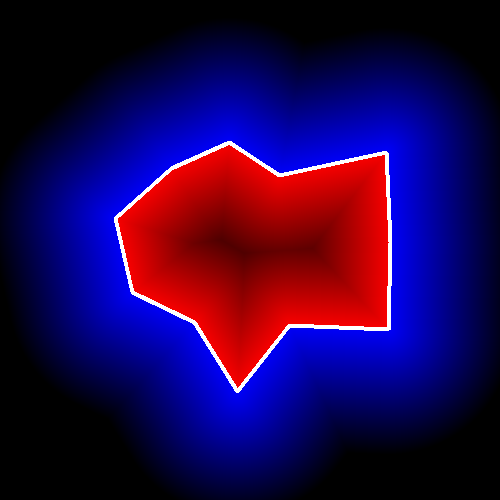
\includegraphics[width=0.5\textwidth]{pics/pointpolygon.png}

\subsection{Object Detection}

\cvfunc{FeatureEvaluator}\label{FeatureEvaluator}
Base class for computing feature values in cascade classifiers

\begin{lstlisting}
class FeatureEvaluator
{
public:    
    // feature type
    enum { HAAR = 0, LBP = 1 };
    virtual ~FeatureEvaluator();
    // reads parameters of the features from a FileStorage node
    virtual bool read(const FileNode& node);
    // returns a full copy of the feature evaluator
    virtual Ptr<FeatureEvaluator> clone() const;
    // returns the feature type (HAAR or LBP for now)
    virtual int getFeatureType() const;
    
    // sets the image in which to compute the features
    // (called by CascadeClassifier::setImage) 
    virtual bool setImage(const Mat& image, Size origWinSize);
    // sets window in the current image in which the features
    // will be computed (called by CascadeClassifier::runAt)
    virtual bool setWindow(Point p);

    // computes value of an ordered (numerical) feature #featureIdx
    virtual double calcOrd(int featureIdx) const;
    // computes value of a categorical feature #featureIdx
    virtual int calcCat(int featureIdx) const;

    // static function that constructs feature evaluator
    // of the specific feature type (HAAR or LBP for now)
    static Ptr<FeatureEvaluator> create(int type);
};
\end{lstlisting}

\cvfunc{CascadeClassifier}\label{CascadeClassifier}
The cascade classifier class for object detection

\begin{lstlisting}
class CascadeClassifier
{
public:    
    enum { BOOST = 0 };

    // default constructor
    CascadeClassifier();
    // load the classifier from file
    CascadeClassifier(const string& filename);
    // the destructor
    ~CascadeClassifier();
    
    // checks if the classifier has been loaded or not
    bool empty() const;
    // loads the classifier from file. The previous content is destroyed.
    bool load(const string& filename);
    // reads the classifier from a FileStorage node.
    bool read(const FileNode& node);
    // detects objects of different sizes in the input image.
    // the detected objects are returned as a list of rectangles.
    // scaleFactor specifies how much the image size is reduced at each image scale.
    // minNeighbors speficifes how many neighbors should
    //        each candiate rectangle have to retain it.
    // flags - ignored
    // minSize - the minimum possible object size. Objects smaller than that are ignored.
    void detectMultiScale( const Mat& image,
                           vector<Rect>& objects,
                           double scaleFactor=1.1,
                           int minNeighbors=3, int flags=0,
                           Size minSize=Size());
    // sets the image for detection (called by detectMultiScale at each image level)
    bool setImage( Ptr<FeatureEvaluator>& feval, const Mat& image );
    // runs the detector at the specified point
    // (the image that the detector is working with should be set
    // by setImage)
    int runAt( Ptr<FeatureEvaluator>& feval, Point pt );

    bool is_stump_based;

    int stageType;
    int featureType;
    int ncategories;
    Size origWinSize;

    Ptr<FeatureEvaluator> feval;
    Ptr<CvHaarClassifierCascade> oldCascade;
};
\end{lstlisting}

\cvfunc{groupRectangles}\label{groupRectangles}
Groups the object candidate rectangles

\begin{lstlisting}
void groupRectangles(vector<Rect>& rectList, int groupThreshold, double eps=0.2);
\end{lstlisting}
\begin{description}
\cvarg{rectList}{The input/output vector of rectangles. On output there will be retained and grouped rectangles}
\cvarg{groupThreshold}{The minimum possible number of rectangles, minus 1, in a group of rectangles to retain it.}
\cvarg{eps}{The relative difference between sides of the rectangles to merge them into a group}
\end{description}

The function is a wrapper for a generic function \cross{partition}. It clusters all the input rectangles using the rectangle equivalence criteria, that combines rectangles that have similar sizes and similar locations (the similarity is defined by \texttt{eps}). When \texttt{eps=0}, no clustering is done at all. If $\texttt{eps}\rightarrow +\inf$, all the rectangles will be put in one cluster. Then, the small clusters, containing less than or equal to \texttt{groupThreshold} rectangles, will be rejected. In each other cluster the average rectangle will be computed and put into the output rectangle list.  

\cvfunc{matchTemplate}\label{matchTemplate}
Compares a template against overlapped image regions.

\begin{lstlisting}
void matchTemplate( const Mat& image, const Mat& templ, Mat& result, int method );

enum { TM_SQDIFF=CV_TM_SQDIFF, TM_SQDIFF_NORMED=CV_TM_SQDIFF_NORMED,
       TM_CCORR=CV_TM_CCORR, TM_CCORR_NORMED=CV_TM_CCORR_NORMED,
       TM_CCOEFF=CV_TM_CCOEFF, TM_CCOEFF_NORMED=CV_TM_CCOEFF_NORMED };
\end{lstlisting}
\begin{description}
\cvarg{image}{Image where the search is running; should be 8-bit or 32-bit floating-point}
\cvarg{templ}{Searched template; must be not greater than the source image and have the same data type}
\cvarg{result}{A map of comparison results; will be single-channel 32-bit floating-point.
If \texttt{image} is $W \times H$ and
\texttt{templ} is $w \times h$ then \texttt{result} will be $(W-w+1) \times (H-h+1)$}
\cvarg{method}{Specifies the comparison method (see below)}
\end{description}

The function \texttt{matchTemplate} slides through \texttt{image}, compares the
overlapped patches of size $w \times h$ against \texttt{templ}
using the specified method and stores the comparison results to
\texttt{result}. Here are the formulas for the available comparison
methods ($I$ denotes \texttt{image}, $T$ \texttt{template},
$R$ \texttt{result}). The summation is done over template and/or the
image patch: $x' = 0...w-1, y' = 0...h-1$

% \texttt{x'=0..w-1, y'=0..h-1}):

\begin{description}
\item[method=CV\_TM\_SQDIFF]
\[ R(x,y)=\sum_{x',y'} (T(x',y')-I(x+x',y+y'))^2 \]

\item[method=CV\_TM\_SQDIFF\_NORMED]
\[ R(x,y)=\frac
{\sum_{x',y'} (T(x',y')-I(x+x',y+y'))^2}
{\sqrt{\sum_{x',y'}T(x',y')^2 \cdot \sum_{x',y'} I(x+x',y+y')^2}}
\]

\item[method=CV\_TM\_CCORR]
\[ R(x,y)=\sum_{x',y'} (T(x',y') \cdot I(x+x',y+y')) \]

\item[method=CV\_TM\_CCORR\_NORMED]
\[ R(x,y)=\frac
{\sum_{x',y'} (T(x',y') \cdot I'(x+x',y+y'))}
{\sqrt{\sum_{x',y'}T(x',y') \cdot \sum_{x',y'} I(x+x',y+y')}}
\]

\item[method=CV\_TM\_CCOEFF]
\[ R(x,y)=\sum_{x',y'} (T'(x',y') \cdot I(x+x',y+y')) \]

where
\[ 
\begin{array}{l}
T'(x',y')=T(x',y') - 1/(w \cdot h) \cdot \sum_{x'',y''} T(x'',y'')\\
I'(x+x',y+y')=I(x+x',y+y') - \frac{1}{(w \cdot h) \cdot \sum_{x'',y''} I(x+x'',y+y'')}
\end{array}
\]

\item[method=CV\_TM\_CCOEFF\_NORMED]
\[ R(x,y)=\frac
{ \sum_{x',y'} (T'(x',y') \cdot I'(x+x',y+y')) }
{ \sqrt{\sum_{x',y'}T'(x',y')^2 \cdot \sum_{x',y'} I'(x+x',y+y')^2} }
\]
\end{description}

After the function finishes the comparison, the best matches can be found as global minimums (when \texttt{CV\_TM\_SQDIFF} was used) or maximums (when \texttt{CV\_TM\_CCORR} or \texttt{CV\_TM\_CCOEFF} was used) using the \cross{minMaxLoc} function. In the case of a color image, template summation in the numerator and each sum in the denominator is done over all of the channels (and separate mean values are used for each channel). That is, the function can take a color template and a color image; the result will still be a single-channel image, which is easier to analyze.


\subsection{Camera Calibration and 3D Reconstruction}

The functions in this section use the so-called pinhole camera model. That
is, a scene view is formed by projecting 3D points into the image plane
using a perspective transformation.

\[
s \quad m' = A [R|t] M'
\]

or

\[
s \vecthree{u}{v}{1} = \vecthreethree
{fx}{0}{cx}
{0}{fy}{cy}
{0}{0}{1}
\begin{bmatrix}
 r_{11} & r_{12} & r{13} & t_1 \\
 r_{21} & r_{22} & r{23} & t_2 \\
 r_{31} & r_{32} & r{33} & t_3
\end{bmatrix}
\begin{bmatrix}X\\Y\\Z\\1 \end{bmatrix}
\]

Where $(X, Y, Z)$ are the coordinates of a 3D point in the world
coordinate space, $(u, v)$ are the coordinates of the projection point
in pixels. $A$ is called a camera matrix, or a matrix of
intrinsic parameters. $(cx, cy)$ is a principal point (that is
usually at the image center), and $fx, fy$ are the focal lengths
expressed in pixel-related units. Thus, if an image from camera is
scaled by some factor, all of these parameters should
be scaled (multiplied/divided, respectively) by the same factor. The
matrix of intrinsic parameters does not depend on the scene viewed and,
once estimated, can be re-used (as long as the focal length is fixed (in
case of zoom lens)). The joint rotation-translation matrix $[R|t]$
is called a matrix of extrinsic parameters. It is used to describe the
camera motion around a static scene, or vice versa, rigid motion of an
object in front of still camera. That is, $[R|t]$ translates
coordinates of a point $(X, Y, Z)$ to some coordinate system,
fixed with respect to the camera. The transformation above is equivalent
to the following (when $z \ne 0$):

\[
\begin{array}{l}
\vecthree{x}{y}{z} = R \vecthree{X}{Y}{Z} + t\\
x' = x/z\\
y' = y/z\\
u = fx*x' + cx\\
v = fy*y' + cy
\end{array}
\]

Real lenses usually have some distortion, mostly
radial distorion and slight tangential distortion. So, the above model
is extended as:

\[
\begin{array}{l}
\vecthree{x}{y}{z} = R \vecthree{X}{Y}{Z} + t\\
x' = x/z\\
y' = y/z\\
x'' = x' (1 + k_1 r^2 + k_2 r^4 + k_3 r^6) + 2 p_1 x' y' + p_2(r^2 + 2 x'^2) \\
y'' = y' (1 + k_1 r^2 + k_2 r^4 + k_3 r^6) + p_1 (r^2 + 2 y'^2) + 2 p_2 x' y' \\
\text{where} \quad r^2 = x'^2 + y'^2 \\
u = fx*x'' + cx\\
v = fy*y'' + cy
\end{array}
\]

$k_1$, $k_2$, $k_3$ are radial distortion coefficients, $p_1$, $p_2$ are tangential distortion coefficients.
Higher-order coefficients are not considered in OpenCV.
The distortion coefficients also do not depend on the scene viewed, thus they are intrinsic camera parameters.
\emph{And they remain the same regardless of the captured image resolution.}
That is, if, for example, a camera has been calibrated on images of $320
\times 240$ resolution, absolutely the same distortion coefficients can
be used for images of $640 \times 480$ resolution from the same camera (while $fx$,
$fy$, $cx$ and $cy$ need to be scaled appropriately).

The functions below use the above model to

\begin{itemize}
 \item Project 3D points to the image plane given intrinsic and extrinsic parameters
 \item Compute extrinsic parameters given intrinsic parameters, a few 3D points and their projections.
 \item Estimate intrinsic and extrinsic camera parameters from several views of a known calibration pattern (i.e. every view is described by several 3D-2D point correspodences).
\end{itemize}


\cvfunc{calibrateCamera}\label{calibrateCamera}
Finds the camera matrix and the camera poses from several views of the calibration pattern.

\begin{lstlisting}
void calibrateCamera( const vector<vector<Point3f> >& objectPoints,
                      const vector<vector<Point2f> >& imagePoints,
                      Size imageSize,
                      Mat& cameraMatrix, Mat& distCoeffs,
                      vector<Mat>& rvecs, vector<Mat>& tvecs,
                      int flags=0 );
enum
{
  CALIB_USE_INTRINSIC_GUESS = CV_CALIB_USE_INTRINSIC_GUESS,
  CALIB_FIX_ASPECT_RATIO = CV_CALIB_FIX_ASPECT_RATIO,
  CALIB_FIX_PRINCIPAL_POINT = CV_CALIB_FIX_PRINCIPAL_POINT,
  CALIB_ZERO_TANGENT_DIST = CV_CALIB_ZERO_TANGENT_DIST,
  CALIB_FIX_FOCAL_LENGTH = CV_CALIB_FIX_FOCAL_LENGTH,
  CALIB_FIX_K1 = CV_CALIB_FIX_K1,
  CALIB_FIX_K2 = CV_CALIB_FIX_K2,
  CALIB_FIX_K3 = CV_CALIB_FIX_K3,
  // only for stereo
  CALIB_FIX_INTRINSIC = CV_CALIB_FIX_INTRINSIC,
  CALIB_SAME_FOCAL_LENGTH = CV_CALIB_SAME_FOCAL_LENGTH,
  // for stereo rectification
  CALIB_ZERO_DISPARITY = CV_CALIB_ZERO_DISPARITY
};
\end{lstlisting}

\begin{description}
\cvarg{objectPoints}{The vector of vectors of points on the calibration rig in its coordinate system, one vector per a view of the rig. If the the same calibration rig is shown in each view and it's fully visible, all the vectors can be the same (though, you may change the numbering from one view to another). The points are 3D, but since they are in the rig coordinate system, then if the rig is planar, it may have sense to put the model to the XY coordinate plane, so that Z-coordinate of each input object point is 0}
\cvarg{imagePoints}{The vector of vectors of the object point projections on the calibration rig views, one vector per a view. The projections must be in the same order as the corresponding object points.}
\cvarg{imageSize}{Size of the image, used only to initialize the intrinsic camera matrix}
\cvarg{cameraMatrix}{The input/output matrix of intrinsic camera parameters $A = \vecthreethree{fx}{0}{cx}{0}{fy}{cy}{0}{0}{1}$. If any of \texttt{CALIB\_USE\_INTRINSIC\_GUESS}, \texttt{CALIB\_FIX\_ASPECT\_RATIO}, \texttt{CALIB\_FIX\_FOCAL\_LENGTH} are specified, some or all of \texttt{fx, fy, cx, cy} must be initialized}
\cvarg{distCoeffs}{The input/output lens distortion coefficients, 4x1, 5x1, 1x4 or 1x5 floating-point vector $k_1, k_2, p_1, p_2[, k_3]$. If any of \texttt{CALIB\_FIX\_K1}, \texttt{CALIB\_FIX\_K2} or \texttt{CALIB\_FIX\_K3} is specified, then the corresponding elements of \texttt{distCoeffs} must be initialized.}
\cvarg{rvecs}{The output vector of rotation vectors (see \cross{Rodrigues}) estimated for each camera view}
\cvarg{tvecsrans}{The output vector of translation vectors estimated for each camera view}
\cvarg{flags}{Different flags, may be 0 or a combination of the following values:
\begin{description}
\cvarg{CALIB\_USE\_INTRINSIC\_GUESS}{\texttt{cameraMatrix} contains the valid initial values of \texttt{fx, fy, cx, cy} that are optimized further. Otherwise, \texttt{(cx, cy)} is initially set to the image center (computed from the input \texttt{imageSize}), and focal distances are computed in some least-squares fashion. Note, that if the focal distance initialization is currently supported only for planar calibration rigs. That is, if the calibration rig is 3D, then you must initialize \texttt{cameraMatrix} and pass \texttt{CALIB\_USE\_INTRINSIC\_GUESS} flag. Also, note that distortion coefficients are not regulated by this function; use \texttt{CALIB\_ZERO\_TANGENT\_DIST} and \texttt{CALIB\_FIX\_K?} to fix them}
\cvarg{CALIB\_FIX\_PRINCIPAL\_POINT}{The principal point is not changed during the global optimization, it stays at the center or, when \texttt{CALIB\_USE\_INTRINSIC\_GUESS} is set too, at the other specified location}
\cvarg{CALIB\_FIX\_ASPECT\_RATIO}{The optimization procedure considers only one of \texttt{fx} and \texttt{fy} as independent variables and keeps the aspect ratio \texttt{fx/fy} the same as it was set initially in the input \texttt{cameraMatrix}. In this case the actual initial values of \texttt{(fx, fy)} are either taken from the matrix (when \texttt{CALIB\_USE\_INTRINSIC\_GUESS} is set) or estimated.}
\cvarg{CALIB\_ZERO\_TANGENT\_DIST}{Tangential distortion coefficients are set to zeros and do not change during the optimization.}
\cvarg{CALIB\_FIX\_FOCAL\_LENGTH}{Both \texttt{fx} and \texttt{fy} are fixed (taken from \texttt{cameraMatrix} and do not change during the optimization.}
\cvarg{CALIB\_FIX\_K1, CALIB\_FIX\_K2, CALIB\_FIX\_K3}{The particular distortion coefficients is read from the input \texttt{distCoeffs} and stays the same during optimization}
\end{description}}
\end{description}

The function \texttt{calibrateCamera} estimates the intrinsic camera
parameters and the extrinsic parameters for each of the views. The
coordinates of 3D object points and their correspondent 2D projections
in each view must be specified. You can use a calibration rig with a known geometry and easily and precisely detectable feature points, e.g. a checkerboard (see \cross{findChessboardCorners}).

The algorithm does the following:
\begin{enumerate}
    \item First, it computes the initial intrinsic parameters (only for planar calibration rigs) or reads them from the input parameters. The distortion coefficients are all set to zeros initially (unless some of \texttt{CALIB\_FIX\_K?} are specified).
    \item The the initial camera pose is estimated as if the intrinsic parameters have been already known. This is done using \cross{solvePnP}
    \item After that the global Levenberg-Marquardt optimization algorithm is run to minimize the reprojection error, i.e. the total sum of squared distances between the observed feature points \texttt{imagePoints} and the projected (using the current estimates for camera parameters and the poses) object points \texttt{objectPoints}; see \cross{projectPoints}.
\end{enumerate}

Note: if you're using a non-square (=non-NxN) grid and
\cross{findChessboardCorners} for calibration, and \texttt{calibrateCamera} returns
bad values (i.e. zero distortion coefficients, an image center very far from
(w/2-0.5,h/2-0.5), and / or large differences between $fx$ and $fy$ (ratios of
10:1 or more)), then you've probaby used \texttt{patternSize=cvSize(rows,cols)},
but should use \texttt{patternSize=cvSize(cols,rows)} in \cross{findChessboardCorners}.

See also: \cross{findChessboardCorners}, \cross{solvePnP}, \cross{initCameraMatrix2D}, \cross{stereoCalibrate}, \cross{undistort}


\cvfunc{calibrationMatrixValues}\label{calibrationMatrixValues}
Computes some useful camera characteristics from the camera matrix

\begin{lstlisting}
void calibrationMatrixValues( const Mat& cameraMatrix,
                              Size imageSize,
                              double apertureWidth,
                              double apertureHeight,
                              double& fovx,
                              double& fovy,
                              double& focalLength,
                              Point2d& principalPoint,
                              double& aspectRatio );
\end{lstlisting}
\begin{description}
\cvarg{cameraMatrix}{The input camera matrix that can be estimated by \cross{calibrateCamera} or \cross{stereoCalibrate}}
\cvarg{imageSize}{The input image size in pixels}
\cvarg{apertureWidth}{Physical width of the sensor}
\cvarg{apertureHeight}{Physical height of the sensor}
\cvarg{fovx}{The output field of view in degrees along the horizontal sensor axis}
\cvarg{fovy}{The output field of view in degrees along the vertical sensor axis}
\cvarg{focalLength}{The focal length of the lens in mm}
\cvarg{prinicialPoint}{The principal point in pixels}
\cvarg{aspectRatio}{\texttt{fy}/texttt{fx}}
\end{description}

The function computes various useful camera characteristics from the previously estimated camera matrix.

\cvfunc{composeRT}\label{composeRT}
Combines two rotation-and-shift transformations

\begin{lstlisting}
void composeRT( const Mat& rvec1, const Mat& tvec1,
                const Mat& rvec2, const Mat& tvec2,
                Mat& rvec3, Mat& tvec3 );
                
void composeRT( const Mat& rvec1, const Mat& tvec1,
                const Mat& rvec2, const Mat& tvec2,
                Mat& rvec3, Mat& tvec3,
                Mat& dr3dr1, Mat& dr3dt1,
                Mat& dr3dr2, Mat& dr3dt2,
                Mat& dt3dr1, Mat& dt3dt1,
                Mat& dt3dr2, Mat& dt3dt2 );
\end{lstlisting}
\begin{description}
\cvarg{rvec1}{The first rotation vector}
\cvarg{tvec1}{The first translation vector}
\cvarg{rvec2}{The second rotation vector}
\cvarg{tvec2}{The second translation vector}
\cvarg{rvec3}{The output rotation vector of the superposition}
\cvarg{tvec3}{The output translation vector of the superposition}
\cvarg{d??d??}{The optional output derivatives of \texttt{rvec3} or \texttt{tvec3} w.r.t. \texttt{rvec?} or \texttt{tvec?}}
\end{description}

The functions compute:

\[ \begin{array}{l}
\texttt{rvec3} = \texttt{Rodrigues}^{(M \rightarrow V)}
    (\texttt{Rodrigues}^{(V \rightarrow M)}{\texttt{rvec2}} \texttt{Rodrigues}^{(V \rightarrow M)}{\texttt{rvec1}}) \\
\texttt{tvec3} = (\texttt{Rodrigues}^{(V \rightarrow M)}{\texttt{rvec2}} \texttt{tvec1} + \texttt{tvec2})
\end{array} \]

and, optionally, the derivatives of the output vectors w.r.t the input vectors (see \cross{matMulDeriv}).
The functions are used inside \cross{stereoCalibrate} but can also be used in your own code where Levenberg-Marquardt or another gradient-based solver is used to optimize a function that contains matrix multiplication.


\cvfunc{computeCorrespondEpilines}\label{computeCorrespondEpilines}
For points in one image of a stereo pair, computes the corresponding epilines in the other image.

\begin{lstlisting}
void computeCorrespondEpilines( const Mat& points,
                                int whichImage, const Mat& F,
                                vector<Vec3f>& lines );
\end{lstlisting}
\begin{description}
\cvarg{points}{The input points. $N \times 1$ or $1 \times N$ matrix of type \texttt{CV\_32FC2} or \texttt{vector<Point2f>}}
\cvarg{whichImage}{Index of the image (1 or 2) that contains the \texttt{points}}
\cvarg{F}{The fundamental matrix that can be estimated using \cross{findFundamentalMat} or \texttt{stereoRectify}}
\cvarg{lines}{The output vector of the corresponding to the points epipolar lines in the other image. Each line $ax + by + c=0$ is encoded as 3-element vector $(a, b, c)$}
\end{description}

For every point in one of the two images of a stereo-pair the function
\texttt{computeCorrespondEpilines} finds the equation of the
corresponding epipolar line in the other image.

From the fundamental matrix definition (see \cross{findFundamentalMatrix}),
line $l^{(2)}_i$ in the second image for the point $p^{(1)}_i$ in the first image (i.e. when \texttt{whichImage=1}) is computed as:

\[ l^{(2)}_i = F p^{(1)}_i \]

and, vice versa, when \texttt{whichImage=2}, $l^{(1)}_i$ is computed from $p^{(2)}_i$ as:

\[ l^{(1)}_i = F^T p^{(2)}_i \]

Line coefficients are defined up to a scale. They are normalized, such that $a_i^2+b_i^2=1$.

\cvfunc{convertPointHomogeneous}\label{convertPointHomogeneous}
Converts 2D points to/from homogeneous coordinates.

\begin{lstlisting}
void convertPointsHomogeneous( const Mat& src, vector<Point3f>& dst );
void convertPointsHomogeneous( const Mat& src, vector<Point2f>& dst );
\end{lstlisting}
\cvarg{src}{The input array or vector of 2D or 3D points}
\cvarg{dst}{The output vector of 3D or 2D points, respectively}
\end{description}

The first of the functions converts 2D points to the homogeneous coordinates by adding extra \texttt{1} component to each point. When the input vector already contains 3D points, it is simply copied to \texttt{dst}. The second function converts 3D points to 2D points by dividing 1st and 2nd components by the 3rd one. If the input vector already contains 2D points, it is simply copied to \texttt{dst}.

\cvfunc{decomposeProjectionMatrix}\label{decomposeProjectionMatrix}
Decomposes the projection matrix into a rotation matrix and a camera matrix.

\begin{lstlisting}
void decomposeProjectionMatrix( const Mat& projMatrix, Mat& cameraMatrix,
                                Mat& rotMatrix, Mat& transVect );
void decomposeProjectionMatrix( const Mat& projMatrix, Mat& cameraMatrix,
                                Mat& rotMatrix, Mat& transVect,
                                Mat& rotMatrixX, Mat& rotMatrixY,
                                Mat& rotMatrixZ, Vec3d& eulerAngles );
\end{lstlisting}
\begin{description}
\cvarg{projMatrix}{The input $3 \times 4$ projection matrix}
\cvarg{cameraMatrix}{The output $3 \times 3$ camera matrix}
\cvarg{rotMatrix}{The output $3 \times 3$ rotation matrix}
\cvarg{transVect}{The output $3 \times 1$ translation vector}
\cvarg{rotMatrixX}{The optional output rotation matrix around x-axis}
\cvarg{rotMatrixY}{The optional output rotation matrix around y-axis}
\cvarg{rotMatrixZ}{The optional output rotation matrix around z-axis}
\cvarg{eulerAngles}{The optional output 3-vector of the Euler rotation angles}
\end{description}

The function \texttt{decomposeProjectionMatrix} computes a decomposition of a projection matrix into a calibration and a rotation matrix and the position of the camera.

It optionally returns three rotation matrices, one for each axis, and the three Euler angles that could be used in OpenGL.

The function is based on \cross{RQDecomp3x3}.

\cvfunc{drawChessboardCorners}\label{drawChessboardCorners}
Draws the detected chessboard corners.

\begin{lstlisting}
void drawChessboardCorners( Mat& image, Size patternSize,
                            const Mat& corners,
                            bool patternWasFound );
\end{lstlisting}
\begin{description}
\cvarg{image}{The destination image; it must be an 8-bit color image}
\cvarg{patternSize}{The number of inner corners per chessboard row and column, i.e. \texttt{Size(<corners per row>, <corners per column>)}}
\cvarg{corners}{The array of detected corners; \texttt{vector<Point2f>} can be passed here as well}
\cvarg{patternWasFound}{Indicates whether the complete board was found. Just pass the return value of \cross{findChessboardCorners} here}
\end{description}

The function \texttt{drawChessboardCorners} draws the detected chessboard corners. If no complete board was found, the detected corners will be marked with small red circles. Otherwise, a colored board (each board row with a different color) will be drawn.

\cvfunc{findFundamentalMat}\label{findFundamentalMat}
Calculates the fundamental matrix from the corresponding points in two images.

\begin{lstlisting}
Mat findFundamentalMat( const Mat& points1, const Mat& points2,
                        vector<uchar>& mask, int method=FM_RANSAC,
                        double param1=3., double param2=0.99 );

Mat findFundamentalMat( const Mat& points1, const Mat& points2,
                        int method=FM_RANSAC,
                        double param1=3., double param2=0.99 );
                        
enum
{ 
    FM_7POINT = CV_FM_7POINT,
    FM_8POINT = CV_FM_8POINT,
    FM_LMEDS = CV_FM_LMEDS,
    FM_RANSAC = CV_FM_RANSAC
};
\end{lstlisting}
\begin{description}
\cvarg{points1}{Array of $N$ points in the first image, a matrix of \texttt{CV\_32FC2} type or \texttt{vector<Point2f>}. The points in homogeneous coordinates can also be passed.}
\cvarg{points2}{Array of the corresponding points in the second image of the same size and the same type as \texttt{points1}}
\cvarg{method}{Method for computing the fundamental matrix
\begin{description}
  \cvarg{FM\_7POINT}{for a 7-point algorithm. $N = 7$}
  \cvarg{FM\_8POINT}{for an 8-point algorithm. $N \ge 8$}
  \cvarg{FM\_RANSAC}{for the RANSAC algorithm. $N \ge 8$}
  \cvarg{FM\_LMEDS}{for the LMedS algorithm. $N \ge 8$}
\end{description}}
\cvarg{param1}{The parameter is used for RANSAC only. It is the maximum distance in pixels from point to epipolar line in pixels, beyond which the point is considered an outlier and is not used for computing the final fundamental matrix. It can be set to something like 1-3, depending on the accuracy of the point localization, image resolution and the image noise}
\cvarg{param2}{The parameter is used for RANSAC or LMedS methods only. It denotes the desirable level of confidence (between 0 and 1) that the estimated matrix is correct}
\cvarg{mask}{The optional output array of $N$ elements, every element of which is set to 0 for outliers and to 1 for the other points. The array is computed only in RANSAC and LMedS methods. Other methods set every element to 1}
\end{description}

The epipolar geometry is described by the following equation:

\[ [p_2; 1]^T F [p_1; 1] = 0 \]

where $F$ is fundamental matrix, $p_1$ and $p_2$ are corresponding points in the first and the second images, respectively.

The function \texttt{findFundamentalMat} calculates the fundamental
matrix using one of four methods listed above and returns the found fundamental matrix. In the case of \texttt{FM\_7POINT} the function may return a $9 \times 3$ matrix. It means that the 3 fundamental matrices are possible and they are all found and stored sequentially.

The calculated fundamental matrix may be passed further to
\texttt{computeCorrespondEpilines} that finds the epipolar lines
corresponding to the specified points. It can also be passed to \cross{stereoRectifyUncalibrated} to compute the rectification transformation.

\begin{lstlisting}
// Example. Estimation of fundamental matrix using RANSAC algorithm
int point_count = 100;
vector<Point2f> points1(point_count);
vector<Point2f> points2(point_count);

// initialize the points here ... */
for( int i = 0; i < point_count; i++ )
{
    points1[i] = ...;
    points2[i] = ...;
}

Mat fundamental_matrix =
 findFundamentalMat(points1, points2, FM_RANSAC, 3, 0.99);
\end{lstlisting}


\cvfunc{findChessboardCorners}\label{findChessboardCorners}
Finds the positions of the internal corners of the chessboard.

\begin{lstlisting}
bool findChessboardCorners( const Mat& image, Size patternSize,
                            vector<Point2f>& corners,
                            int flags=CV_CALIB_CB_ADAPTIVE_THRESH+
                                 CV_CALIB_CB_NORMALIZE_IMAGE );
enum { CALIB_CB_ADAPTIVE_THRESH = CV_CALIB_CB_ADAPTIVE_THRESH,
    CALIB_CB_NORMALIZE_IMAGE = CV_CALIB_CB_NORMALIZE_IMAGE,
    CALIB_CB_FILTER_QUADS = CV_CALIB_CB_FILTER_QUADS };
\end{lstlisting}
\begin{description}
\cvarg{image}{The input chessboard (a.k.a. checkerboard) view; it must be an 8-bit grayscale or color image}
\cvarg{patternSize}{The number of inner corners per chessboard row and column, i.e.
\texttt{patternSize = cvSize(<points per row>, <points per column>)}}
\cvarg{corners}{The output vector of the corners detected. If the board is found (the function returned true), the corners should be properly ordered.}
\cvarg{flags}{Various operation flags, can be 0 or a combination of the following values:
\begin{description}
 \cvarg{CALIB\_CB\_ADAPTIVE\_THRESH}{use adaptive thresholding, instead of a fixed-level threshold, to convert the image to black and white rather than a fixed threshold level}
 \cvarg{CALIB\_CB\_NORMALIZE\_IMAGE}{normalize the image brightness and contrast using \cross{equalizeHist} before applying fixed or adaptive thresholding}
 \cvarg{CALIB\_CB\_FILTER\_QUADS}{use some additional criteria (like contour area, perimeter, square-like shape) to filter out false quads that are extracted at the contour retrieval stage. Since the current corner grouping engine is smart enough, usually this parameter is omitted.}
\end{description}}
\end{description}

The function \texttt{findChessboardCorners} attempts to determine
whether the input image is a view of the chessboard pattern and, if yes,
locate the internal chessboard corners. The function returns true if all
of the chessboard corners have been found and they have been placed
in a certain order (row by row, left to right in every row),
otherwise, if the function fails to find all the corners or reorder
them, it returns 0. For example, a regular chessboard has 8 x 8
squares and 7 x 7 internal corners, that is, points, where the black
squares touch each other. The coordinates detected are approximate,
and to determine their position more accurately, the user may use
the function \cross{cornerSubPix} or other subpixel adjustment technique.

Sometimes the function fails to find the board because the image is too large or too small. If so, try to resize it and then scale the found corners coordinates back (or even scale the computed \texttt{cameraMatrix} back).


\cvfunc{getDefaultNewCameraMatrix}\label{getDefaultNewCameraMatrix}
Returns the default new camera matrix

\begin{lstlisting}
Mat getDefaultNewCameraMatrix( const Mat& cameraMatrix, Size imgSize=Size(),
                               bool centerPrincipalPoint=false );
\end{lstlisting}
\begin{description}
\cvarg{cameraMatrix}{The input camera matrix}
\cvarg{imageSize}{The camera view image size in pixels}
\cvarg{centerPrincipalPoint}{Indicates whether in the new camera matrix the principal point should be at the image center or not}
\end{description}

The function returns the camera matrix that is either an exact copy of the input \texttt{cameraMatrix} (when \texttt{centerPrinicipalPoint=false}), or the modified one (when \texttt{centerPrincipalPoint}=true).

In the latter case the new camera matrix will be:

\[\begin{bmatrix}
f_x && 0 && (\texttt{imgSize.width}-1)*0.5 \\
0 && f_y && (\texttt{imgSize.height}-1)*0.5 \\
0 && 0 && 1
\end{bmatrix},\]

where $f_x$ and $f_y$ are $(0,0)$ and $(1,1)$ elements of \texttt{cameraMatrix}, respectively.

By default, the undistortion functions in OpenCV (see \texttt{initUndistortRectifyMap}, \texttt{undistort}) do not move the principal point. However, when you work with stereo, it's important to move the principal points in both views to the same y-coordinate (which is required by most of stereo correspondence algorithms), and maybe to the same x-coordinate too. So you can form the new camera matrix for each view, where the principal points will be at the center. 

\cvfunc{initCameraMatrix2D}\label{initCameraMatrix2D}
Finds the initial camera matrix from the 3D-2D point correspondences

\begin{lstlisting}
Mat initCameraMatrix2D( const vector<vector<Point3f> >& objectPoints,
                        const vector<vector<Point2f> >& imagePoints,
                        Size imageSize, double aspectRatio=1. );
\end{lstlisting}
\begin{description}
\cvarg{objectPoints}{The vector of vectors of the object points. See \cross{calibrateCamera}}
\cvarg{imagePoints}{The vector of vectors of the corresponding image points. See \cross{calibrateCamera}}
\cvarg{imageSize}{The image size in pixels; used to initialize the principal point}
\cvarg{aspectRatio}{If it is zero or negative, both $f_x$ and $f_y$ are estimated independently. Otherwise $f_x = f_y * \texttt{aspectRatio}$}
\end{description}

The function estimates and returns the initial camera matrix for camera calibration process.
Currently, the function only supports planar calibration rigs, i.e. the rig for which the $3 \times 3$ covariance matrix of object points is singular.


\cvfunc{Rodrigues}\label{Rodrigues}
Converts a rotation matrix to a rotation vector or vice versa.

\begin{lstlisting}
void Rodrigues(const Mat& src, Mat& dst);
void Rodrigues(const Mat& src, Mat& dst, Mat& jacobian);
\end{lstlisting}

\begin{description}
\cvarg{src}{The input rotation vector (3x1 or 1x3) or a rotation matrix (3x3)}
\cvarg{dst}{The output rotation matrix (3x3) or a rotation vector (3x1 or 1x3), respectively}
\cvarg{jacobian}{The optional output Jacobian matrix, 3x9 or 9x3 - partial derivatives of the output array components with respect to the input array components}
\end{description}

The functions convert a rotation vector to a rotation matrix or vice versa. A rotation vector is a compact representation of rotation matrix. Direction of the rotation vector is the rotation axis and the length of the vector is the rotation angle around the axis. The rotation matrix $R$, corresponding to the rotation vector $r$, is computed as following:

\[
\begin{array}{l}
\theta \leftarrow norm(r)\\
r \leftarrow r/\theta\\
R = \cos{\theta} I + (1-\cos{\theta}) r r^T + \sin{\theta}
\vecthreethree
{0}{-r_z}{r_y}
{r_z}{0}{-r_x}
{-r_y}{r_x}{0}
\end{array}
\]

Inverse transformation can also be done easily as

\[
\sin(\theta)
\vecthreethree
{0}{-r_z}{r_y}
{r_z}{0}{-r_x}
{-r_y}{r_x}{0}
=
\frac{R - R^T}{2}
\]

A rotation vector is a convenient and most-compact representation of a rotation matrix
(since any rotation matrix has just 3 degrees of freedom). The representation is
used in the global 3D geometry optimization procedures like \cross{calibrateCamera}, \cross{stereoCalibrate} or \cross{solvePnP}.


\cvfunc{RQDecomp3x3}\label{RQDecomp3x3}
Computes the 'RQ' decomposition of 3x3 matrices.

\begin{lstlisting}
/* Computes RQ decomposition for 3x3 matrices */
void RQDecomp3x3( const Mat& M, Mat& R, Mat& Q );
Vec3d RQDecomp3x3( const Mat& M, Mat& R, Mat& Q,
                   Mat& Qx, Mat& Qy, Mat& Qz );
\end{lstlisting}
\begin{description}
\cvarg{M}{The input $3 \times 3$ floating-point matrix}
\cvarg{R}{The output $3 \times 3$ upper-triangular matrix}
\cvarg{Q}{The output $3 \times 3$ orthogonal matrix}
\cvarg{Qx, Qy, Qz}{The optional output matrices that decompose the rotation matrix Q into separate rotation matrices for each coordinate axis}
\end{description}

The function \texttt{RQDecomp3x3} implements RQ decomposition of a $3 \times 3$ matrix. The function is by \cross{decomposeProjectionMatrix}.

\cvfunc{matMulDeriv}\label{matMulDeriv}
Computes partial derivatives of the matrix product w.r.t each multiplied matrix

\begin{lstlisting}
void matMulDeriv( const Mat& A, const Mat& B, Mat& dABdA, Mat& dABdB );
\end{lstlisting}
\begin{description}
\cvarg{A}{The first multiplied matrix}
\cvarg{B}{The second multiplied matrix}
\cvarg{dABdA}{The first output derivative matrix \texttt{d(A*B)/dA} of size $\texttt{A.rows*B.cols} \times {A.rows*A.cols}$}
\cvarg{dABdA}{The second output derivative matrix \texttt{d(A*B)/dB} of size $\texttt{A.rows*B.cols} \times {B.rows*B.cols}$}
\end{description}

The function computes the partial derivatives of the elements of the matrix product $A*B$ w.r.t. the elements of each of the two input matrices. The function is used to compute Jacobian matrices in \cross{stereoCalibrate}, but can also be used in any other similar optimization function.

\cvfunc{projectPoints}\label{projectPoints}
Projects 3D points on to an image plane.

\begin{lstlisting}
void projectPoints( const Mat& objectPoints,
                    const Mat& rvec, const Mat& tvec,
                    const Mat& cameraMatrix,
                    const Mat& distCoeffs,
                    vector<Point2f>& imagePoints );

void projectPoints( const Mat& objectPoints,
                    const Mat& rvec, const Mat& tvec,
                    const Mat& cameraMatrix,
                    const Mat& distCoeffs,
                    vector<Point2f>& imagePoints,
                    Mat& dpdrot, Mat& dpdt, Mat& dpdf,
                    Mat& dpdc, Mat& dpddist,
                    double aspectRatio=0 );
\end{lstlisting}
\begin{description}
\cvarg{objectPoints}{The input array of 3D object points, a matrix of type \texttt{CV\_32FC3} or \texttt{vector<Point3f>}}
\cvarg{imagePoints}{The output array of 2D image points}
\cvarg{rvec}{The rotation vector, 1x3 or 3x1}
\cvarg{tvec}{The translation vector, 1x3 or 3x1}
\cvarg{cameraMatrix}{The camera matrix $\vecthreethree{f_x}{0}{c_x}{0}{f_y}{c_y}{0}{0}{1}$}
\cvarg{distCoeffs}{The array of distortion coefficients, 4x1, 5x1, 1x4 or 1x5 $k_1, k_2, p_1, p_2[, k_3]$. If the matrix is empty, the function uses zero distortion coefficients}
\cvarg{dpdrot, dpdt, dpdf, dpdc, dpdist}{The optional matrices of the partial derivatives of the computed point projections w.r.t the rotation vector, the translation vector, $f_x$ and $f_y$, $c_x$ and $c_y$ and the distortion coefficients respectively. Each matrix has $2*N$ rows (where $N$ is the number of points) - even rows (0th, 2nd ...) are the derivatives of the x-coordinates w.r.t. the camera parameters and odd rows (1st, 3rd ...) are the derivatives of the y-coordinates.}
\cvarg{aspectRatio}{If zero or negative, $f_x$ and $f_y$ are treated as independent variables, otherwise they $f_x = f_y*\texttt{aspectRatio}$, so the derivatives are adjusted appropriately}
\end{description}

The function \texttt{projectPoints} computes projections of 3D
points to the image plane given intrinsic and extrinsic camera
parameters. Optionally, the function computes jacobians - matrices
of partial derivatives of image points as functions of all the
input parameters with respect to the particular camera parameters, intrinsic and/or
extrinsic. The computed jacobians are used during the global optimization
in \cross{calibrateCamera}, \cross{stereoCalibrate} and \cross{solvePnP}.

Note, that by setting \texttt{rvec=tvec=(0,0,0)} or by setting \texttt{cameraMatrix=Mat::eye(3,3,CV\_64F)} or by setting \texttt{distCoeffs=Mat()} you can get various useful partial cases of the function, i.e. you can computed the distorted coordinates for a sparse set of points, or apply a perspective transformation (and also compute the derivatives) in the ideal zero-distortion setup etc.

\cvfunc{reprojectImageTo3D}\label{reprojectImageTo3D}
Reprojects disparity image to 3D space.

\begin{lstlisting}
void reprojectImageTo3D( const Mat& disparity,
                         Mat& _3dImage, const Mat& Q,
                         bool handleMissingValues=false );
\end{lstlisting}
\begin{description}
\cvarg{disparity}{The input single-channel 16-bit signed or 32-bit floating-point disparity image}
\cvarg{\_3dImage}{The output 3-channel floating-point image of the same size as \texttt{disparity}.
 Each element of \texttt{\_3dImage(x,y)} will contain the 3D coordinates of the point \texttt{(x,y)}, computed from the disparity map.}
\cvarg{Q}{The $4 \times 4$ perspective transformation matrix that can be obtained with \cross{stereoRectify}}
\cvarg{handleMissingValues}{If true, when the pixels with the minimal disparity (that corresponds to the ouliers; see \cross{StereoBM}) will be transformed to 3D points with some very large Z value (currently set to 10000)}
\end{description}
 
The function transforms 1-channel disparity map to 3-channel image representing a 3D surface. That is, for each pixel \texttt{(x,y)} and the corresponding disparity \texttt{d=disparity(x,y)} it computes: 

\[\begin{array}{l}
[X Y Z W]^T = \texttt{Q}*[x y \texttt{disparity}(x,y) 1]^T \\
\texttt{\_3dImage}(x,y) = (X/W, Y/W, Z/W)
\end{array}\]

The matrix \texttt{Q} can be arbitrary $4 \times 4$ matrix, e.g. the one computed by \cross{stereoRectify}. To reproject a sparse set of points {(x,y,d),...} to 3D space, use \cross{perspectiveTransform}.  


\cvfunc{solvePnP}\label{solvePnP}
Finds the camera pose from the 3D-2D point correspondences

\begin{lstlisting}
void solvePnP( const Mat& objectPoints,
               const Mat& imagePoints,
               const Mat& cameraMatrix,
               const Mat& distCoeffs,
               Mat& rvec, Mat& tvec,
               bool useExtrinsicGuess=false );
\end{lstlisting}
\begin{description}
\cvarg{objectPoints}{The array of object points, a matrix of type \texttt{CV\_32FC3} or \texttt{vector<Point3f>}}
\cvarg{imagePoints}{The array of the corresponding image points, a matrix of type{CV\_32FC2} or \texttt{vector<Point2f>}}
\cvarg{cameraMatrix}{The input camera matrix $\vecthreethree{f_x}{0}{c_x}{0}{f_y}{c_y}{0}{0}{1}$}
\cvarg{distCoeffs}{The input 4x1, 5x1, 1x4 or 1x5 array of distortion coefficients $(k_1, k_2, p_1, p_2[, k3])$. If it is NULL, all of the distortion coefficients are set to 0}
\cvarg{rvec}{The output camera view rotation vector (compact representation of a rotation matrix, \cross{Rodrigues} that (together with \texttt{tvec}) brings points from the model coordinate system to the camera coordinate system}
\cvarg{tvec}{The output camera view translation vector}
\end{description}

The function \texttt{solvePnP} estimates the camera pose given a set of object points, their corresponding image projections, as well as the camera matrix and the distortion coefficients. This function finds such a pose that minimizes back-projection error, i.e. the sum of squared distances between the observed projections \texttt{imagePoints} and the projected with \cross{projectPoints} \texttt{objectPoints}.

\cvfunc{stereoCalibrate}\label{stereoCalibrate}
Calibrates stereo camera.

\begin{lstlisting}
void stereoCalibrate( const vector<vector<Point3f> >& objectPoints,
                      const vector<vector<Point2f> >& imagePoints1,
                      const vector<vector<Point2f> >& imagePoints2,
                      Mat& cameraMatrix1, Mat& distCoeffs1,
                      Mat& cameraMatrix2, Mat& distCoeffs2,
                      Size imageSize, Mat& R, Mat& T,
                      Mat& E, Mat& F,
                      TermCriteria criteria = TermCriteria(TermCriteria::COUNT+
                         TermCriteria::EPS, 30, 1e-6),
                      int flags=CALIB_FIX_INTRINSIC );
\end{lstlisting}
\begin{description}
\cvarg{objectPoints}{The vector of vectors of points on the calibration rig in its coordinate system, one vector per a view of the rig. See \cross{calibrateCamera}}
\cvarg{imagePoints1}{The vector of vectors of the object point projections to the first camera views, one vector per a view. The projections must be in the same order as the corresponding object points.}
\cvarg{imagePoints2}{The vector of vectors of the object point projections to the second camera views, one vector per a view. The projections must be in the same order as the corresponding object points.}
\cvarg{imageSize}{Size of the image, used only to initialize the intrinsic camera matrices}
\cvarg{cameraMatrix1, cameraMatrix2}{The input/output first and second camera matrices, respectively: $ \vecthreethree{f_x^{(j)}}{0}{c_x^{(j)}}{0}{f_y^{(j)}}{c_y^{(j)}}{0}{0}{1}$, $j = 0,\, 1$. If any of \texttt{CALIB\_USE\_INTRINSIC\_GUESS}, \texttt{CALIB\_FIX\_ASPECT\_RATIO},
\texttt{CALIB\_FIX\_INTRINSIC} or \texttt{CALIB\_FIX\_FOCAL\_LENGTH} are specified, some or all of the matrices' components must be initialized}
\cvarg{distCoeffs1, distCoeffs2}{The input/output lens distortion coefficients for the first and the second cameras, 4x1, 5x1, 1x4 or 1x5 floating-point vectors $k_1^{(j)}, k_2^{(j)}, p_1^{(j)}, p_2^{(j)}[, k_3^{(j)}]$, $j = 0,\, 1$. If any of \texttt{CALIB\_FIX\_K1}, \texttt{CALIB\_FIX\_K2} or \texttt{CALIB\_FIX\_K3} is specified, then the corresponding elements of the distortion coefficients must be initialized.}
\cvarg{R}{The output rotation matrix between the 1st and the 2nd cameras' coordinate systems.}
\cvarg{T}{The output translation vector between the cameras' coordinate systems.}
\cvarg{E}{The output essential matrix.}
\cvarg{F}{The output fundamental matrix.}
\cvarg{criteria}{The termination criteria for the iterative optimiziation algorithm.}
\cvarg{flags}{Different flags, may be 0 or combination of the following values:
\begin{description}
\cvarg{CALIB\_FIX\_INTRINSIC}{If it is set, \texttt{cameraMatrix?}, as well as \texttt{distCoeffs?} are fixed, so that only \texttt{R, T, E} and \texttt{F} are estimated.}
\cvarg{CALIB\_USE\_INTRINSIC\_GUESS}{The flag allows the function to optimize some or all of the intrinsic parameters, depending on the other flags, but the initial values are provided by the user.}
\cvarg{CALIB\_FIX\_PRINCIPAL\_POINT}{The principal points are fixed during the optimization.}
\cvarg{CALIB\_FIX\_FOCAL\_LENGTH}{$f^{(j)}_x$ and $f^{(j)}_y$ are fixed.}
\cvarg{CALIB\_FIX\_ASPECT\_RATIO}{$f^{(j)}_y$ is optimized, but the ratio $f^{(j)}_x/f^{(j)}_y$ is fixed.}
\cvarg{CALIB\_SAME\_FOCAL\_LENGTH}{Enforces $f^{(0)}_x=f^{(1)}_x$ and $f^{(0)}_y=f^{(1)}_y$} \cvarg{CALIB\_ZERO\_TANGENT\_DIST}{Tangential distortion coefficients for each camera are set to zeros and fixed there.}
\cvarg{CALIB\_FIX\_K1, CALIB\_FIX\_K2, CALIB\_FIX\_K3}{Fixes the corresponding radial distortion coefficient (the coefficient must be passed to the function)}
\end{description}}
\end{description}

The function \texttt{stereoCalibrate} estimates transformation between the 2 cameras - heads of a stereo pair. If we have a stereo camera, where the relative position and orientatation of the 2 cameras is fixed, and if we computed poses of an object relative to the fist camera and to the second camera, $(R^{(1)}, T^{(1)})$ and $(R^{(2)}, T^{(2)})$, respectively (that can be done with \cross{solvePnP}), then, obviously, those poses will relate to each other, by knowing only one of $(R^{(j)}, T^{(j)})$ we can compute the other one:

\[\begin{array}{l}
R^{(2)}=R*R^{(1)} \\
T^{(2)}=R*T^{(1)} + T,
\end{array}
\]

And, vice versa, if we computed both $(R^{(1)}, T^{(1)})$ and $(R^{(2)}, T^{(2)})$, we can compute the relative position and orientation of the 2 cameras as following:

\[\begin{array}{l}
R=R^{(2)} {R^{(1)}}^{-1} \\
T=T^{(2)} - R^{(2)} {R^{(1)}}^{-1}*T^{(1)}
\end{array}
\]

The function uses this idea, but the actual algorithm is more complex to take all the available pairs of the camera views into account.

Also, the function computes the essential matrix \texttt{E}:

\[
E=
\vecthreethree
{0}{-T_2}{T_1}
{T_2}{0}{-T_0}
{-T_1}{T_0}{0}
*R,
\]

where $T_i$ are components of the translation vector $T:\,T=[T_0, T_1, T_2]^T$,
and the fundamental matrix \texttt{F}:

\[F = cameraMatrix2^{-T} E cameraMatrix1^{-1}\]

Besides the stereo-related information, the function can also perform full calibration of each of the 2 cameras. However, because of the high dimensionality of the parameter space and noise in the input data the function can diverge from the correct solution. Thus, if the intrinsic parameters can be estimated with high accuracy for each of the cameras individually (e.g. using \cross{calibrateCamera}), it is recommended to do so and then pass \texttt{CALIB\_FIX\_INTRINSIC} flag to the function along with the computed intrinsic parameters. Otherwise, if all the parameters are needed to be estimated at once, it makes sense to restrict some parameters, e.g. pass \texttt{CALIB\_SAME\_FOCAL\_LENGTH} and \texttt{CALIB\_ZERO\_TANGENT\_DIST} flags, which are usually reasonable assumptions. 


\cvfunc{stereoRectify}\label{stereoRectify}
Computes rectification transforms for each head of a calibrated stereo camera.

\begin{lstlisting}
void stereoRectify( const Mat& cameraMatrix1, const Mat& distCoeffs1,
                    const Mat& cameraMatrix2, const Mat& distCoeffs2,
                    Size imageSize, const Mat& R, const Mat& T,
                    Mat& R1, Mat& R2, Mat& P1, Mat& P2, Mat& Q,
                    int flags=CALIB_ZERO_DISPARITY );
\end{lstlisting}
\begin{description}
\cvarg{cameraMatrix1, cameraMatrix2}{The camera matrices [$f_x^{(j)}$ 0 $c_x^{(j)}$; 0 $f_y^{(j)}$ $c_y^{(j)}$; 0 0 1].}
\cvarg{distCoeffs1, distCoeffs2}{The vectors of distortion coefficients for each camera, \href{\#Pinhole Camera Model, Distortion}{4x1, 1x4, 5x1 or 1x5.}}
\cvarg{imageSize}{Size of the image used for stereo calibration.}
\cvarg{R}{The input rotation matrix between the 1st and the 2nd cameras' coordinate systems; can be computed with \cross{stereoCalibrate}.}
\cvarg{T}{The translation vector between the cameras' coordinate systems; can be computed with \cross{stereoCalibrate}.}
\cvarg{R1, R2}{The output $3 \times 3$ rectification transforms (rotation matrices) for the first and the second cameras, respectively.}
\cvarg{P1, P2}{The output $3 \times 4$ projection matrices in the new (rectified) coordinate systems.}
\cvarg{Q}{The output $4 \times 4$ disparity-to-depth mapping matrix, see \cross{reprojectImageTo3D}.}
\cvarg{flags}{The operation flags; may be 0 or \texttt{CALIB\_ZERO\_DISPARITY}. If the flag is set, the function makes the principal points of each camera have the same pixel coordinates in the rectified views. And if the flag is not set, the function may still shift the images in horizontal or vertical direction (depending on the orientation of epipolar lines) in order to maximize the useful image area.}
\end{description}

The function \texttt{stereoRectify} computes the rotation matrices for each camera that (virtually) make both camera image planes the same plane. Consequently, that makes all the epipolar lines parallel and thus simplifies the dense stereo correspondence problem. On input the function takes the matrices computed by \cross{stereoCalibrate} and on output it gives 2 rotation matrices and also 2 projection matrices in the new coordinates. The 2 cases are distinguished by the function are: 

\begin{enumerate}
\item{Horizontal stereo, when 1st and 2nd camera views are shifted relative to each other mainly along the x axis (with possible small vertical shift). Then in the rectified images the corresponding epipolar lines in left and right cameras will be horizontal and have the same y-coordinate. P1 and P2 will look as: 

\[
\texttt{P1}=
\begin{bmatrix}
f & 0 & cx_1 & 0\\
0 & f & cy & 0\\
0 & 0 & 1 & 0
\end{bmatrix}
\]
\[
\texttt{P2}=
\begin{bmatrix}
f & 0 & cx_2 & T_x*f\\
0 & f & cy & 0\\
0 & 0 & 1 & 0
\end{bmatrix}
,
\]

where $T_x$ is horizontal shift between the cameras and $cx_1=cx_2$ if \texttt{CALIB\_ZERO\_DISPARITY} is set.}
\item{Vertical stereo, when 1st and 2nd camera views are shifted relative to each other mainly in vertical direction (and probably a bit in the horizontal direction too). Then the epipolar lines in the rectified images will be vertical and have the same x coordinate. P2 and P2 will look as:

\[
P1=
\begin{bmatrix}
f & 0 & cx & 0\\
0 & f & cy_1 & 0\\
0 & 0 & 1 & 0
\end{bmatrix}
\]
\[
P2=
\begin{bmatrix}
f & 0 & cx & 0\\
0 & f & cy_2 & T_y*f\\
0 & 0 & 1 & 0
\end{bmatrix}
,
\]

where $T_y$ is vertical shift between the cameras and $cy_1=cy_2$ if \texttt{CALIB\_ZERO\_DISPARITY} is set.}
\end{enumerate} 

As you can see, the first 3 columns of \texttt{P1} and \texttt{P2} will effectively be the new "rectified" camera matrices. 
The matrices, together with \texttt{R1} and \texttt{R2}, can then be passed to \cross{initUndistortRectifyMap} to initialize the rectification map for each camera.  

\cvfunc{stereoRectifyUncalibrated}\label{stereoRectifyUncalibrated}
Computes rectification transforms for each head of an uncalibrated stereo camera.

\begin{lstlisting}
bool stereoRectifyUncalibrated( const Mat& points1,
                                const Mat& points2,
                                const Mat& F, Size imgSize,
                                Mat& H1, Mat& H2,
                                double threshold=5 );
\end{lstlisting}
\begin{description}
\cvarg{points1, points2}{The two arrays of corresponding 2D points.}
\cvarg{F}{Fundamental matrix. It can be computed using the same set of point pairs \texttt{points1} and \texttt{points2}  using \cross{findFundamentalMat}.}
\cvarg{imageSize}{Size of the image.}
\cvarg{H1, H2}{The output rectification homography matrices for the first and for the second images.}
\cvarg{threshold}{Optional threshold used to filter out the outliers. If the parameter is greater than zero, then all the point pairs that do not comply the epipolar geometry well enough (that is, the points for which $|\texttt{points2[i]}^T*\texttt{F}*\texttt{points1[i]}|>\texttt{threshold}$) are rejected prior to computing the homographies.}
\end{description}

The function \texttt{stereoRectifyUncalibrated} computes the rectification transformations without knowing intrinsic parameters of the cameras and their relative position in space, hence the suffix "Uncalibrated". Another related difference from \cross{stereoRectify} is that the function outputs not the rectification transformations in the object (3D) space, but the planar perspective transformations, encoded by the homography matrices \texttt{H1} and \texttt{H2}. The function implements the following algorithm \href{\#Hartly99}{[Hartley99]}. 

Note that while the algorithm does not need to know the intrinsic parameters of the cameras, it heavily depends on the epipolar geometry. Therefore, if the camera lenses have significant distortion, it would better be corrected before computing the fundamental matrix and calling this function. For example, distortion coefficients can be estimated for each head of stereo camera separately by using \cross{calibrateCamera} and then the images can be corrected using \cross{undistort}, or just the point coordinates can be corrected with \cross{undistortPoints}. 

\cvfunc{StereoBM}\label{StereoBM}
The class for computing stereo correspondence using block matching algorithm.

\begin{lstlisting}
// Block matching stereo correspondence algorithm
class StereoBM
{
    enum { NORMALIZED_RESPONSE = CV_STEREO_BM_NORMALIZED_RESPONSE,
        BASIC_PRESET=CV_STEREO_BM_BASIC,
        FISH_EYE_PRESET=CV_STEREO_BM_FISH_EYE,
        NARROW_PRESET=CV_STEREO_BM_NARROW };
    
    StereoBM();
    // the preset is one of ..._PRESET above.
    // ndisparities is the size of disparity range,
    // in which the optimal disparity at each pixel is searched for.
    // SADWindowSize is the size of averaging window used to match pixel blocks
    //    (larger values mean better robustness to noise, but yield blurry disparity maps)
    StereoBM(int preset, int ndisparities=0, int SADWindowSize=21);
    // separate initialization function
    void init(int preset, int ndisparities=0, int SADWindowSize=21);
    // computes the disparity for the two rectified 8-bit single-channel images.
    // the disparity will be 16-bit singed image of the same size as left.
    void operator()( const Mat& left, const Mat& right, Mat& disparity );

    Ptr<CvStereoBMState> state;
};
\end{lstlisting}

\cvfunc{undistortPoints}\label{undistortPoints}
Computes the ideal point coordinates from the observed point coordinates.

\begin{lstlisting}
void undistortPoints( const Mat& src, vector<Point2f>& dst,
                      const Mat& cameraMatrix, const Mat& distCoeffs,
                      const Mat& R=Mat(), const Mat& P=Mat());
void undistortPoints( const Mat& src, Mat& dst,
                      const Mat& cameraMatrix, const Mat& distCoeffs,
                      const Mat& R=Mat(), const Mat& P=Mat());
\end{lstlisting}
\begin{description}
\cvarg{src}{The observed point coordinates, a matrix or vector of 2D points.}
\cvarg{dst}{The ideal point coordinates, after undistortion and reverse perspective transformation}
\cvarg{cameraMatrix}{The camera matrix $[f_x 0 c_x; 0 f_y c_y; 0 0 1]$}
\cvarg{distCoeffs}{he vector of distortion coefficients, \cross{4x1, 1x4, 5x1 or 1x5}}
\cvarg{R}{The rectification transformation in object space (3x3 matrix). \texttt{R1} or \texttt{R2}, computed by \cross{StereoRectify} can be passed here. If the matrix is empty, the identity transformation is used}
\cvarg{P}{The new camera matrix (3x3) or the new projection matrix (3x4). \texttt{P1} or \texttt{P2}, computed by \cross{StereoRectify} can be passed here. If the matrix is empty, the identity new camera matrix is used}
\end{description}

The function \texttt{undistortPoints} is similar to \cross{undistort} and \cross{initUndistortRectifyMap}, but it operates on a sparse set of points instead of a raster image. Also the function does some kind of reverse transformation to \cross{projectPoints} (in the case of 3D object it will not reconstruct its 3D coordinates, of course; but for a planar object it will, up to a translation vector, if the proper \texttt{R} is specified).

%\include{CvAux-cpp}
\chapter{C++. HighGUI}

While OpenCV was designed for use in full-scale
applications and can be used within functionally rich UI frameworks (such as Qt, WinForms or Cocoa) or without any UI at all, sometimes there is a need to try some functionality quickly and visualize the results. This is what the HighGUI module has been designed for.

It provides easy interface to:
\begin{itemize}
    \item create and manipulate windows that can display images and "remember" their content (no need to handle repaint events from OS)
    \item add trackbars to the windows, handle simple mouse events as well as keyboard commmands
    \item read and write images to/from disk or memory.
    \item read video from camera or file and write video to a file.
\end{itemize}

\section{The Reference}

\subsection{User Interface}

\cvfunc{createTrackbar}\label{createTrackbar}

\begin{lstlisting}
int createTrackbar( const string& trackbarname, const string& winname,
                    int* value, int count,
                    TrackbarCallback onChange CV_DEFAULT(0),
                    void* userdata CV_DEFAULT(0));
\end{lstlisting}
\begin{description}
\cvarg{trackbarname}{Name of the created trackbar.}
\cvarg{winname}{Name of the window which will be used as a parent of the created trackbar.}
\cvarg{value}{The optional pointer to an integer variable, whose value will reflect the position of the slider. Upon creation, the slider position is defined by this variable.}
\cvarg{count}{The maximal position of the slider. The minimal position is always 0.}
\cvarg{onChange}{Pointer to the function to be called every time the slider changes position. This function should be prototyped as \texttt{void Foo(int,void*);}, where the first parameter is the trackbar position and the second parameter is the user data (see the next parameter). If the callback is NULL pointer, then no callbacks is called, but only \texttt{value} is updated}
\cvarg{userdata}{The user data that is passed as-is to the callback; it can be used to handle trackbar events without using global variables}
\end{description}

The function \texttt{createTrackbar} creates a trackbar (a.k.a. slider or range control) with the specified name and range, assigns a variable \texttt{value} to be syncronized with trackbar position and specifies a callback function \texttt{onChange} to be called on the trackbar position change. The created trackbar is displayed on the top of the given window.

\cvfunc{getTrackbarPos}\label{getTrackbarPos}
Returns the trackbar position.

\begin{lstlisting}
int getTrackbarPos( const string& trackbarname, const string& winname );
\end{lstlisting}
\begin{description}
\cvarg{trackbarname}{Name of the trackbar.}
\cvarg{winname}{Name of the window which is the parent of the trackbar.}
\end{description}

The function returns the current position of the specified trackbar.

\cvfunc{imshow}\label{imshow}
Displays the image in the specified window

\begin{lstlisting}
void imshow( const string& winname, const Mat& image );
\end{lstlisting}
\begin{description}
\cvarg{winname}{Name of the window.}
\cvarg{image}{Image to be shown.}
\end{description}

The function \texttt{imshow} displays the image in the specified window. If the window was created with the \texttt{CV\_WINDOW\_AUTOSIZE} flag then the image is shown with its original size, otherwise the image is scaled to fit in the window. The function may scale the image, depending on its depth:
\begin{itemize}
    \item If the image is 8-bit unsigned, it is displayed as is.
    \item If the image is 16-bit unsigned or 32-bit integer, the pixels are divided by 256. That is, the value range [0,255*256] is mapped to [0,255].
    \item If the image is 32-bit floating-point, the pixel values are multiplied by 255. That is, the value range [0,1] is mapped to [0,255].
\end{itemize}


\cvfunc{namedWindow}\label{namedWindow}
Creates a window.

\begin{lstlisting}
void namedWindow( const string& winname, int flags );
\end{lstlisting}
\begin{description}
\cvarg{name}{Name of the window in the window caption that may be used as a window identifier.}
\cvarg{flags}{Flags of the window. Currently the only supported flag is \texttt{CV\_WINDOW\_AUTOSIZE}. If this is set, the window size is automatically adjusted to fit the displayed image (see \cross{imshow}), and the user can not change the window size manually.}
\end{description}

The function \texttt{namedWindow} creates a window which can be used as a placeholder for images and trackbars. Created windows are referred to by their names.

If a window with the same name already exists, the function does nothing.

\cvfunc{setTrackbarPos}\label{setTrackbarPos}
Sets the trackbar position.

\begin{lstlisting}
void setTrackbarPos( const string& trackbarname, const string& winname, int pos );
\end{lstlisting}
\begin{description}
\cvarg{trackbarname}{Name of the trackbar.}
\cvarg{winname}{Name of the window which is the parent of trackbar.}
\cvarg{pos}{The new position.}
\end{description}

The function sets the position of the specified trackbar in the specified window.


\cvfunc{waitKey}\label{waitKey}
Waits for a pressed key.

\begin{lstlisting}
int waitKey(int delay=0);
\end{lstlisting}
\begin{description}
\cvarg{delay}{Delay in milliseconds. 0 is the special value that means "forever"}
\end{description}

The function \texttt{waitKey} waits for key event infinitely (when $\texttt{delay}\leq 0$) or for \texttt{delay} milliseconds, when it's positive. Returns the code of the pressed key or -1 if no key was pressed before the specified time had elapsed.

\textbf{Note:} This function is the only method in HighGUI that can fetch and handle events, so it needs to be called periodically for normal event processing, unless HighGUI is used within some environment that takes care of event processing.


\subsection{Image and Video I/O}

\cvfunc{imdecode}\label{imdecode}

\begin{lstlisting}
Mat imdecode( const Mat& buf, int flags );
\end{lstlisting}
\begin{description}
\cvarg{buf}{The input array of vector of bytes}
\cvarg{flags}{The same flags as in \cross{imread}}
\end{description}

The function reads image from the specified buffer in memory.
If the buffer is too short or contains invalid data, the empty matrix will be returned.

See \cross{imread} for the list of supported formats and the flags description. 

\cvfunc{imencode}\label{imencode}

\begin{lstlisting}
bool imencode( const string& ext, const Mat& img,
               vector<uchar>& buf,
               const vector<int>& params=vector<int>());
\end{lstlisting}
\begin{description}
\cvarg{ext}{The file extension that defines the output format}
\cvarg{img}{The image to be written}
\cvarg{buf}{The output buffer; resized to fit the compressed image}
\cvarg{params}{The format-specific parameters; see \cross{imwrite}}
\end{description}

The function compresses the image and stores it in the memory buffer, which is resized to fit the result.
See \cross{imwrite} for the list of supported formats and the flags description.


\cvfunc{imread}\label{imread}
Loads an image from a file.

\begin{lstlisting}
Mat imread( const string& filename, int flags=1 );

#define CV_LOAD_IMAGE_COLOR       1
#define CV_LOAD_IMAGE_GRAYSCALE   0
#define CV_LOAD_IMAGE_UNCHANGED  -1
\end{lstlisting}

\begin{description}
\cvarg{filename}{Name of file to be loaded.}
\cvarg{flags}{Specifies color type of the loaded image: if $>$0, the loaded image is forced to be a 3-channel color image; if 0, the loaded image is forced to be grayscale; if $<$0, the loaded image will be loaded as is (note that in the current implementation the alpha channel, if any, is stripped from the output image, e.g. 4-channel RGBA image will be loaded as RGB).}
\end{description}

The function \texttt{imread} loads an image from the specified file and returns it. Currently, the following file formats are supported:
\begin{itemize}
\item Windows bitmaps - \texttt{*.bmp, *.dib} (always supported)
\item JPEG files - \texttt{*.jpeg, *.jpg, *.jpe} (see \textbf{Note2})
\item JPEG 2000 files - \texttt{*.jp2} (see \textbf{Note2})
\item Portable Network Graphics - \texttt{*.png}  (see \textbf{Note2})
\item Portable image format - \texttt{*.pbm, *.pgm, *.ppm} (always supported)
\item Sun rasters - \texttt{*.sr, *.ras} (always supported)
\item TIFF files - \texttt{*.tiff, *.tif}  (see \textbf{Note2})
\end{itemize}

\textbf{Note1}: The function determines type of the image by the content, not by the file extension.

\textbf{Note2}: On Windows and MacOSX the shipped with OpenCV image codecs (libjpeg, libpng, libtiff and libjasper) are used by default; so OpenCV can always read JPEGs, PNGs and TIFFs. On MacOSX there is also the option to use native MacOSX image readers. But beware that currently these native image loaders give images with somewhat different pixel values, because of the embedded into MacOSX color management.

On Linux, BSD flavors and other Unix-like open-source operating systems OpenCV looks for the supplied with OS image codecs. Please, install the relevant packages (do not forget the development files, e.g. "libjpeg-dev" etc. in Debian and Ubuntu) in order to get the codec support, or turn on \texttt{OPENCV\_BUILD\_3RDPARTY\_LIBS} flag in CMake. 

\cvfunc{imwrite}\label{imwrite}
Saves an image to a specified file.

\begin{lstlisting}
bool imwrite( const string& filename, const Mat& img,
              const vector<int>& params=vector<int>());
#define CV_IMWRITE_JPEG_QUALITY 1
#define CV_IMWRITE_PNG_COMPRESSION 16
#define CV_IMWRITE_PXM_BINARY 32
\end{lstlisting}
\begin{description}
\cvarg{filename}{Name of the file.}
\cvarg{img}{The image to be saved.}
\cvarg{params}{The format-specific save parameters, encoded as pairs \texttt{paramId\_1, paramValue\_1, paramId\_2, paramValue\_2, ...}. The following parameters are currently supported:
\begin{itemize}
    \item In the case of JPEG it can be a quality (\texttt{CV\_IMWRITE\_JPEG\_QUALITY}), from 0 to 100 (the higher is the better), 95 by default.
    \item In the case of PNG it can be the compression level (\texttt{CV\_IMWRITE\_PNG\_COMPRESSION}), from 0 to 9 (the higher value means smaller size and longer compression time), 3 by default.
    \item In the case of PPM, PGM or PBM it can a binary format flag (\texttt{CV\_IMWRITE\_PXM\_BINARY}), 0 or 1, 1 by default.
\end{itemize}
    }
\end{description}

The function \texttt{imwrite} saves the image to the specified file. The image format is chosen based on the \texttt{filename} extension, see \cross{imread} for the list of extensions. Only 8-bit (or 16-bit in the case of PNG, JPEG 2000 and TIFF) single-channel or 3-channel (with 'BGR' channel order) images can be saved using this function. If the format, depth or channel order is different, use \cross{Mat::convertTo}, and \cross{cvtColor} to convert it before saving, or use the universal XML I/O functions to save the image to XML or YAML format.

\cvfunc{VideoCapture}\label{VideoCapture}
Class for video capturing from video files or cameras

\begin{lstlisting}
class VideoCapture
{
public:
    // the default constructor
    VideoCapture();
    // the constructor that opens video file
    VideoCapture(const string& filename);
    // the constructor that starts streaming from the camera
    VideoCapture(int device);
    
    // the destructor
    virtual ~VideoCapture();
    
    // opens the specified video file
    virtual bool open(const string& filename);
    
    // starts streaming from the specified camera by its id
    virtual bool open(int device);
    
    // returns true if the file was open successfully or if the camera
    // has been initialized succesfully
    virtual bool isOpened() const;
    
    // closes the camera stream or the video file
    // (automatically called by the destructor)
    virtual void release();
    
    // grab the next frame or a set of frames from a multi-head camera;
    // returns false if there are no more frames
    virtual bool grab();
    // reads the frame from the specified video stream
    // (non-zero channel is only valid for multi-head camera live streams)
    virtual bool retrieve(Mat& image, int channel=0);
    // equivalent to grab() + retrieve(image, 0);
    virtual VideoCapture& operator >> (Mat& image);
    
    // sets the specified property propId to the specified value 
    virtual bool set(int propId, double value);
    // retrieves value of the specified property
    virtual double get(int propId);
    
protected:
    ...
};
\end{lstlisting}

See \hyperref[AutomaticMemoryManagement2]{the CXCORE introduction} for the sample code.

\cvfunc{VideoWriter}\label{VideoWriter}
Video writer class

\begin{lstlisting}
class VideoWriter
{
public:    
    // default constructor
    VideoWriter();
    // constructor that calls open
    VideoWriter(const string& filename, int fourcc,
                double fps, Size frameSize, bool isColor=true);
    
    // the destructor
    virtual ~VideoWriter();
    
    // opens the file and initializes the video writer.
    // filename - the output file name. 
    // fourcc - the codec
    // fps - the number of frames per second
    // frameSize - the video frame size
    // isColor - specifies whether the video stream is color or grayscale
    virtual bool open(const string& filename, int fourcc,
                      double fps, Size frameSize, bool isColor=true);
    
    // returns true if the writer has been initialized successfully
    virtual bool isOpened() const;
    
    // writes the next video frame to the stream
    virtual VideoWriter& operator << (const Mat& image);
    
protected:
    ...
};
\end{lstlisting}

\chapter{FAQ}
\section{First Section}
\subsection{Initialization}

\subsubsection*{CreateImage}
\addcontentsline{toc}{subsubsection}{CreateImage} 

Creates header and \textsf{allocates} data

\begin{shaded}
\begin{verbatim}
IplImage* cvCreateImage( CvSize size,
                         int depth,
                         int channels );
\end{verbatim}
\end{shaded}

\begin{description}
\item[\texttt{size}] Image width and height
\item[\texttt{depth}] Bit depth of image elements.  Can be one of:
\begin{description}
\item[IPL\_DEPTH\_8U] unsigned 8-bit integers
\item[IPL\_DEPTH\_8S] signed 8-bit integers
\item[IPL\_DEPTH\_16U] unsigned 16-bit integers
\item[IPL\_DEPTH\_16S] signed 16-bit integers
\item[IPL\_DEPTH\_32S] signed 32-bit integers
\item[IPL\_DEPTH\_32F] single precision floating-point numbers
\item[IPL\_DEPTH\_64F] double precision floating-point numbers
\end{description}
\item[\texttt{channels}] Number of channels per element(pixel). Can be 1, 2, 3 or 4. The channels are interleaved, for example the usual data layout of a color image is:
\begin{lstlisting}
b0 g0 r0 b1 g1 r1 ...
\end{lstlisting}
Although in general IPL image format can store non-interleaved images as well and some of OpenCV can process it, this function can create interleaved images only.

\end{description}

The function cvCreateImage creates the header and allocates data as in the method of~\cite{author_conf_year}.  This call is a shortened form of 
\begin{lstlisting}
header = cvCreateImageHeader(size,depth,channels);
cvCreateData(header);
\end{lstlisting}

%%%%%%%%%%%%%%%%


\bibliographystyle{plain}
{\small
\bibliography{opencv}
}

\printindex


\end{document}             % End of document.
